\chapter{Examples: Multivariate Special Functions}


\section{Functions Of Matrix Arguments}
\label{FunctionsOfMatrixArguments}



\subsection{\texorpdfstring{$\text{Multivariate Gamma function }\Gamma_p(x)$}{Multivariate Gamma}}
\nomenclature{$\Gamma_p(x)$}{Multivariate Gamma Function}
\label{MultivariateGammaFunction} 


\begin{mpFunctionsExtract}
	\mpFunctionTwoNotImplemented
	{Gammap? mpNum? the multivariate gamma function.}
	{p? mpNum? An integer greater than 0.}
	{x? mpNum? A real number or an array of real numbers.}	
\end{mpFunctionsExtract}


\vspace{0.3cm}
The multivariate gamma function is defined by
\begin{equation}
	\Gamma_p(x)  = \pi^{p(p-1)/4} \prod_{i=1}^p \Gamma\left(x-\tfrac{1}{2}(i-1)\right), \quad \Re(x) > \tfrac{1}{2}(m-1)
\end{equation}
\begin{equation}
	\Gamma_p(s_1,\ldots,s_p)  = \pi^{p(p-1)/4} \prod_{i=1}^p \Gamma\left(s_i-\tfrac{1}{2}(i-1)\right), \quad \Re(s_i) > \tfrac{1}{2}(i-1), \quad j=1,\ldots,m.
\end{equation}
\begin{equation}
	\Gamma_p(a,\ldots,a)  = \Gamma_p(a)
\end{equation}

where $\Gamma(\cdot)$ is the usual (scalar) gamma funcion (see section \ref{GammaFunction}).





\newpage
\subsection{Zonal Polynomials}
\label{ZonalPolynomials}

\subsubsection{Definitions}
A partition $\kappa = (k_1 , . . . , k_m)$ is a vector of nonnegative integers, listed in nonincreasing order. Also, $|\kappa|$ denotes $k_1 + \cdots +k_m$ , the weight of $\kappa$; $\ell(\kappa)$ denotes the number of nonzero $k_j$ ; $a+\kappa$ denotes the vector $(a+k_1,\ldots, a+k_m )$.

The partitional shifted factorial is given by \citep{NIST}
\begin{equation}
	\left[a\right]_{\kappa} = \frac{\Gamma_m(a+\kappa)}{\Gamma_m(a)} = \prod_{j=1} \left(a-\tfrac{1}{2}(j-1) \right)_{k_j},
\end{equation} \\
where $(a)_k$ is the Pochammer symbol 
(see section \ref{PochhammerSymbol}).

For any partition $\kappa$, the zonal polynomial $Z_{\kappa} : \textbf{S} \rightarrow \mathbb{R}$ is defined by the properties \citep{NIST}
\begin{equation}
	Z_{\kappa}(\textbf{I}) = |\kappa|!2^{2|\kappa|} \left[m/2 \right]_{\kappa} \frac{\prod\limits_{1\leq j < l \leq \ell(\kappa)} (2k_j-2k_l-j+l)}{\prod\limits_{j=1}^{\ell(\kappa)} (2k_j+\ell(\kappa)-j)!}, \quad \text{and}
\end{equation} 
\begin{equation}
	Z_{\kappa}(\textbf{T}) = Z_{\kappa}(\textbf{I}) |\textbf{T}|^{k_m} \int_{\textbf{O}(m)} \prod_{j=1}^{m-1} |(\textbf{HTH}^{-1})_j|^{k_j-k_{j+1}} d\textbf{H}
\end{equation} 
See \cite{Muirhead_1982}, pp. 68-72, for the definition and properties of the Haar measure $d\textbf{H}$. Alternative notations for the zonal polynomials are $C_{\kappa}(\textbf{T})$ \cite{Muirhead_1982}, pp. 227-239.

\subsubsection{Properties}
Zonal polynomials have the following properties \citep{NIST}:
\begin{equation}
	Z_{\kappa}(0) = \begin{cases}
		1, & \kappa=(0,\ldots,0),\\
		0, & \kappa\neq(0,\ldots,0).
	\end{cases}
\end{equation} 
\begin{equation}
	Z_{\kappa}(\textbf{HTH}^{-1}) = Z_{\kappa}(\textbf{T}), \quad \textbf{H} \in \textbf{O}(m).
\end{equation} 
Therefore $Z_{\kappa}(\textbf{T})$ is a symmetric polynomial in the eigenvalues of $\textbf{T}$. Also, for $k=0,1,2,\ldots,$
\begin{equation}
	\sum_{|\kappa|=k} Z_{\kappa}(\textbf{T}) = (\text{tr}\textbf{T})^k.
\end{equation} 

\subsubsection{Implementation}
\cite{Gupta_1979} describe an algorithm for the calculation of zonal polynomials for $2\times 2$ and $3 \times 3$ matrices.


\cite{James_1964, James_1968, McLaren_1976} descibe a general algorithm.









\newpage
\subsection{Gauss Hypergeometric Function of Matrix Argument}
\label{sec:Hypergeometric2F2Matrix}
\nomenclature{${}_2F_1(a,b;c;\textbf{T})$}{Gauss Hypergeometric Function of Matrix Argument}


\begin{mpFunctionsExtract}
	\mpFunctionFourNotImplemented
	{Hypergeometric2F1Matrix? mpNum? the Gauss hypergeometric function for matrix argument.}
	{a? mpNum? A real number.}
	{b? mpNum? A real number.}	
	{c? mpNum? A real number.}
	{T? mpNum? A real matrix.}	
\end{mpFunctionsExtract}


\vspace{0.3cm}


The Gauss hypergeometric function for matrix argument, ${}_2F_1(a, b; c; \textbf{T})$ is defined by \citep{NIST}

\begin{equation}
	{}_2F_1(a,b;c;\textbf{T}) = \sum_{k=0}^\infty \frac{1}{k!}  \sum_{|\kappa|=k}  \frac{\left[a\right]_{\kappa}\left[b\right]_{\kappa}}{\left[c\right]_{\kappa}} Z_{\kappa}(\textbf{T})
\end{equation}
with $-c+\tfrac{1}{2}(j+1) \notin  \mathbb{N}, 1 \leq j \leq m; ||\textbf{T}||<1$. Here $Z_{\kappa}(\textbf{T})$ is a zonal polynomial, as described in section \ref{ZonalPolynomials}.

See also \cite{Koev_2006} for an "exact" calculation.


\subsubsection{Laplace approximation}
The following closed-form approximation based on a Laplace approximation has been derived by \cite{Butler_Wood_2002}:
\begin{equation}
	{}_2{F}_1(a,b;c;X)  \approx \frac{c^{pc-p(p+1)/4}}{\sqrt{R_{2,1}}}   \times \prod_{i=1}^p \left[\left(\frac{y_i}{a}\right)^a \left(\frac{1-y_i}{c-a} \right)^{c-a} (1-x_i y_i)^{-b}  \right],
\end{equation}
\begin{center}
	where $X=\text{diag}(x_1,\ldots,x_p)$, $S_i = x_i y_i (1-y_i)/(1-x_i y_i)$, $\tau_i = x_i(b-a)-c$,
\end{center}
\begin{equation*}
	y_i=\frac{2a}{\sqrt{t_i^2 - 4ax_i(c-b)}-\tau_i}, \text{ and } R_{2,1} = \prod_{i=1}^p  \prod_{j=i}^p \left[\frac{y_i y_j}{a}+\frac{(1-y_i)(1-y_j)}{c-a}-\frac{b}{a(c-a)} S_i S_j   \right]. 
\end{equation*}












\newpage
\subsection{Confluent Hypergeometric Function for Matrix Argument}
\nomenclature{${}_1F_1(a,b;\Omega)$}{Kummer's Confluent Hypergeometric Function for Matrix Argument}
\label{Hypergeometric1F1Matrix}


\begin{mpFunctionsExtract}
	\mpFunctionThreeNotImplemented
	{Hypergeometric1F1Matrix? mpNum? Kummer's confluent hypergeometric function  for matrix argument.}
	{a? mpNum? A real number.}
	{b? mpNum? A real number.}	
	{T? mpNum? A real matrix.}	
\end{mpFunctionsExtract}


\vspace{0.3cm}
Kummer's confluent hypergeometric function  for matrix argument ${}_1F_1(a;b;\textbf{T})$ is defined by the series \citep{NIST}

\begin{equation}
	{}_1F_1(a;b;\textbf{T}) = \sum_{k=0}^\infty \frac{1}{k!}  \sum_{|\kappa|=k}  \frac{\left[a\right]_{\kappa}}{\left[b\right]_{\kappa}} Z_{\kappa}(\textbf{T})
\end{equation}
with $-b+\tfrac{1}{2}(j+1) \notin  \mathbb{N}, 1 \leq j \leq m$. Here $Z_{\kappa}(\textbf{T})$ is a zonal polynomial, as described in section \ref{ZonalPolynomials}.


See also \cite{Koev_2006} for an "exact" calculation.

\subsubsection{Laplace approximation}
The following closed-form approximation based on a Laplace approximation has been derived by \cite{Butler_Wood_2002}, with $X=\text{diag}(x_1,\ldots,x_p)$:

\begin{equation}
	{}_1{F}_1(a;b;X)  \approx \frac{b^{pb-p(p+1)/4}}{\sqrt{R_{1,1}}}  \times \prod_{i=1}^p \left[\left(\frac{y_i}{a}\right)^a \left(\frac{1-y_i}{b-a} \right)^{b-a} e^{x_i y_i}  \right],
\end{equation}
\begin{equation*}
	\text{where } y_i=\frac{2a}{b-x_i+\sqrt{(x_i-b)^2 + 4ax_i}}, \text{ and } R_{1,1} = \prod_{i=1}^p  \prod_{j=i}^p \left[\frac{y_i y_j}{a}+\frac{(1-y_i)(1-y_j)}{b-a}\right]. 
\end{equation*}












\newpage
\subsection{Confluent Hypergeometric Limit Function for Matrix Argument}
\nomenclature{${}_0F_1(a;\Omega)$}{Confluent Hypergeometric Limit Function for Matrix Argument}
\label{Hypergeometric0F1Matrix}


\begin{mpFunctionsExtract}
	\mpFunctionTwoNotImplemented
	{Hypergeometric0F1Matrix? mpNum? the confluent hypergeometric limit function for matrix argument.}
	{n? mpNum? A real number.}
	{T? mpNum? A real matrix.}	
\end{mpFunctionsExtract}


\vspace{0.3cm}
This functions returns the confluent hypergeometric limit function for matrix argument ${}_0F_1(a; X)$, defined by the series \citep{NIST,Butler_Wood_2003}

\begin{equation}
	{}_0F_1(\tfrac{1}{2}n;\tfrac{1}{4}XX^{\text{T}}) = \sum_{k=0}^\infty \frac{1}{k!}  \sum_{|\kappa|=k}  \frac{1}{\left[\tfrac{1}{2}n\right]_{\kappa}} Z_{\kappa}(\textbf{X})
\end{equation}
Here $Z_{\kappa}(\textbf{X})$ is a zonal polynomial, as described in section \ref{ZonalPolynomials}.



\subsubsection{Laplace approximation}
The following closed-form approximation based on a Laplace approximation has been derived by \cite{Butler_Wood_2003}, with $X=\text{diag}(x_1,\ldots,x_p)$:

\begin{equation}
	{}_0{F}_1 \left(\tfrac{1}{2}n;\tfrac{1}{4}XX^{\text{T}} \right)  \approx \frac{1}{\sqrt{R_{0,1}}}  \times \prod_{i=1}^p \left[(1-y_i)^{n/2} e^{x_i y_i}  \right],
\end{equation}
\begin{equation*}
	\text{where } y_i=\frac{2x_i/n}{\sqrt{(2x_i/n)^2 + 1}+1}, \text{ and } R_{0,1} = \prod_{i=1}^p  \prod_{j=i}^p (1-y_i^2 y_j^2). 
\end{equation*}





\chapter{Examples: Moments, cumulants, and expansions}


\section{Moments and cumulants}
\label{Moments and cumulants}

The following relations hold between central moments, cumulants, and moments about the origin:

Central moments from null moments: 
\begin{equation}
	\mu_n = \sum_{j=0}^n \binom{n}{j} (-1)^{n-j} \mu_j'(\mu_1)^{n-j}
\end{equation}


Null moments from central moments: 
\begin{equation}
	\mu_n' = \sum_{r=0}^n \binom{n}{r} (\mu_1)^{r}
\end{equation}


Cumulants  from null moments: 
\begin{equation}
	\kappa_r = \mu_r' - \sum_{j=1}^{r-1} \binom{r-1}{j-1} \mu_{r-j}' \kappa_j
\end{equation}


Cumulants  from central moments: 
\begin{equation}
	\kappa_r = \mu_r - \sum_{j=2}^{r-1} \binom{r-1}{j-1} \mu_{r-j} \kappa_j, \quad r>1, \quad \kappa_1=\mu_1.
\end{equation}



\vspace{0.6cm}

\begin{mpFunctionsExtract}
	\mpFunctionOneNotImplemented
	{CentralMomentsToRawMoments? mpNum? raw moments calculated from central moments.}
	{Central? mpNum? A real vector.}
\end{mpFunctionsExtract}


\vspace{0.6cm}

\begin{mpFunctionsExtract}
	\mpFunctionOneNotImplemented
	{RawMomentsToCentralMoments? mpNum? central moments calculated from raw moments.}
	{Raw? mpNum? A real vector.}
\end{mpFunctionsExtract}


\vspace{0.6cm}

\begin{mpFunctionsExtract}
	\mpFunctionOneNotImplemented
	{CentralMomentsToCumulants? mpNum? cumulants calculated from central moments.}
	{Central? mpNum? A real vector.}
\end{mpFunctionsExtract}


\vspace{0.6cm}

\begin{mpFunctionsExtract}
	\mpFunctionOneNotImplemented
	{CumulantsToCentralMoments? mpNum? central moments calculated from cumulants.}
	{Cumulants? mpNum? A real vector.}
\end{mpFunctionsExtract}


\vspace{0.6cm}

\begin{mpFunctionsExtract}
	\mpFunctionOneNotImplemented
	{RawMomentsToCumulants? mpNum? cumulants calculated from raw moments.}
	{Raw? mpNum? A real vector.}	
\end{mpFunctionsExtract}


\vspace{0.6cm}

\begin{mpFunctionsExtract}
	\mpFunctionOneNotImplemented
	{CumulantsToRawMoments? mpNum? raw moments calculated from cumulants.}
	{Cumulants? mpNum? A real vector.}
\end{mpFunctionsExtract}





\newpage
\section{The Edgeworth expansion}

\subsection{Continuous variates}

Many distribution function can be approximated by an expansion of the normal distribution, provided that the cumulants of the distribution are known \citep{Lee_1992}.
\begin{equation}
	f(x) = \phi(x) + \sum_{i=1}^{\infty} \sum_{\pi(i)} \omega_{\pi(i)} Z^{(D(\pi(i)))}(x)
\end{equation}
\begin{equation}
	F(x) = \Phi(x) + \sum_{i=1}^{\infty} \sum_{\pi(i)} \omega_{\pi(i)} Z^{(D(\pi(i))-1)}(x)
\end{equation}
where the summation is extended over the partitions
\begin{equation}
	\pi(i) = \left(s_1^{m_1},\ldots,s_k^{m_k}\right) \text{ such that } s_1 > \ldots > s_k \text{ and } i = \sum_{i=1}^k{m_k s_k},
\end{equation}
\begin{equation}
	\omega_{\pi(i)} = \prod_{i=1}^k \frac{\gamma_{s_i}^{m_i}}{m_i !}, \quad \gamma_i = \frac{(-1)^i \kappa_i}{\sqrt{\kappa_2^i}(i+2)!}, \text{ and } D(\pi(i)) = \sum_{i=1}^k m_i (s_i +2).
\end{equation}
Using the first 4 cumulants, we have
\begin{equation}
	\text{Pr}\left[\frac{u-\mu}{\sigma}\right] = \Phi(x) + \phi(x)\left[\frac{\gamma_1}{6}(1-x^2) + \frac{\gamma_2}{24}(3x-x^3) +  \frac{\gamma_1^2}{72}(15x-10x^3+x^5)\right] + O(N^{-3/2}) 
\end{equation}


\subsubsection{Wilks, Hotelling's T2, Pillai's V}


Example: moments of T2: \cite{Davis_1968} , equation 7.13

moments of V:  \cite{Davis_1970a} Davis 1970, equation 2.11 (and section 4).

Box-omega of V:\cite{Davis_1970a}, equations 5.2 to 5.4 

Box-omega of T2: \cite{Davis_1970a}, equations 5.6, and \cite{Davis_1970b}, equations 3.10 to 3.11



\subsection{Lattice (discrete) variates}




Decribe formula for Kendall's tau.

\newpage
\section{The Cornish-Fisher expansion}

Many distribution function can be approximated by an expansion of the normal distribution, provided that the cumulants of the distribution are known. Cornish and Fisher derived an inversion formula \citep{fisher_percentile_1960}, which has been generalized by \cite{Lee_1992}.


Lee's algorithm is based on the following formula for the adjustment of order $n^{-k/2}$:
\begin{equation}
	\delta_k = a_k H^{k+1} + \sum_{(\kappa*)} \frac{(-1)^{\pi}}{j_1!\ldots j_m!} \left(\delta_{k_1} - a_{k_1} H^{k_1+1}\right)^{j_1} \ldots \left(\delta_{k_m} - a_{k_m} H^{k_m+1}\right)^{j_m} H^{\pi-1} \label{eq:LeeCornishFisher}
\end{equation}
where $\delta_i$ is the $i$th-order adjustment (of magnitude $O(n^{i/2})$), $a_i=\kappa_i/i! \sigma^i$, where $\kappa_i$ is the $i$th cumulant, and $(\kappa*)$ is the set of all partitions of $k$ having two or more parts. The typical term shown in the summand is due to the partition having $j_1$ occurrences of $k_1$ and so on; $\pi$ is the number of parts in the partition; and the powers of $H$ are to be multiplied out formally, with $H^j$ replaced by the Hermite polynomial $H_j(z)$ (with $z$ representing the normal deviate) in the final result.
A recurrence formula connects the $\delta_k(H)$:
\begin{equation}
	\delta_k' = a_k' H^{k+1} + \sum_{j=1}^{k-1} \binom{k-1}{j} \delta_{k-1}' (H) (\delta_j' - a_j' H^{j+1}),
\end{equation}
where $\delta_h'(H) = h! \delta_h(H), \delta_h'=h!\delta_h, a_h'=h!h_h$ and $\delta_h(H)$ means an expression like the right-hand side of equation (\ref{eq:LeeCornishFisher}), formally a polynomial in $H$, and $\delta_h$ is a numerical value. In this formula the adjustment of a given order is calculated recursively, the values of lower order adjustments being used in each stage of calculation.



Using the first 4 cumulants, we have
\begin{equation}
	u = \mu + \sigma \left[z + \frac{\gamma_1}{6}(z^2-1) + \frac{\gamma_2}{24}(z^3 - 3z) -  \frac{\gamma_1^2}{36}(2z^3-5z)\right] + O(N^{-3/2}) 
\end{equation}






\newpage
\section{Saddlepoint approximations}
%Huang(2011) gives the following formulas:
%
%Dating back to Esscher (1932), the saddlepoint approximation has been recognized
%as a valuable tool in asymptotic analysis and statistical computing. It has
%found a wide range of applications in finance and insurance, reliability theory,
%physics and biology. The saddlepoint approximation literature so far mainly focuses
%on the approximation of densities (Daniels, 1954) and tail probabilities
%(Lugannani \& Rice (1980) and Daniels (1987)). For a comprehensive exposition
%of saddlepoint approximations, see Jensen (1995).

%\vspace{0.3cm}
Suppose the moment generating function (MGF) of the random variable $X$ is analytic and given by $M(t)$ for $t$ in some open
neighborhood of zero. Let $K(t)$ = $\log (M(t))$  be the Cumulant Generating Function(CGF) of $X$, and denote by $K'(t)$, $K''(t)$, $K^{(3)}(t)$ and $K^{(4)}(t)$ the 
first, second, third and fourth derivative of $K(t)$, respectively. Let $F(x)$ and $f(x)$ denote the CDF and pdf of $X$, respectively, and $\Phi(\cdot)$ and $\phi(\cdot)$ denote the CDF (see section \ref{sec:NormalDistribution_CDF}) and pdf (see section \ref{sec:NormalDistribution_pdf}) of the normal distribution, respectively.


Let $s$ be the solution to the saddlepoint equation 
\begin{equation} 
	K'(s)=x. \label{eq:saddlepoint_s}
\end{equation}
which in general needs to be solved numerically (sometimes closed form solutions exist), and define

\begin{equation}
	w = w(s) = \text{sgn}(s) \sqrt{2 (s K'(s) - K(s))} \label{eq:saddlepoint_w}
\end{equation}


\begin{equation}
	u = u(s) = s \sqrt{K''(s)}  \label{eq:saddlepoint_u}
\end{equation}


\begin{equation}
	r = r(s) = w(s) + \frac{1}{w(s)} \log \frac{u(s)}{w(s)}  \label{eq:saddlepoint_r}
\end{equation}



\subsection{First order approximations}
Add: formulas for $s=0$.

\cite{Jensen_1992} gives the following formula:
\begin{equation}
	F(x)   \thickapprox   \Phi(r) =: P1.  \label{eq:saddlepoint_Jensen}
\end{equation}




\cite{LugannaniRice_1980} give the following formula: 

\begin{equation}
	F(x)   \thickapprox   \Phi(w)+\phi(w)\left( \frac{1}{w} - \frac{1}{u} \right) =: P3.
\end{equation}




\subsection{Second order approximations}


\cite{Daniels_1954,Daniels_1987} gives the following formulas:

\begin{equation}
	F(x)   \thickapprox   P3+\phi(w) \left(\frac{\kappa_4}{8u} - \frac{5}{24u}\kappa_3^2 - \frac{1}{u^3} - \frac{\kappa_3}{2u^2}+ \frac{1}{w^3} \right) =:P4,
\end{equation}


\begin{equation}
	f(x)   \thickapprox \phi(w) \frac{s}{u}  \left(1+\frac{\kappa_4}{8} - \frac{5}{24}\kappa_3^2 \right), \quad \text{where}
\end{equation}

\begin{equation}
	\kappa_3 = K^{(3)}(s) / K''(s) ^ {3/2} \quad \kappa_4 = K^{(4)}(s) / K''(s)^2
\end{equation}





\newpage
\section{Inverse Saddlepoint approximations}

We assume that we have defined a function $F_s(x)$ to convert from $x$ to $s$ , and also an inverse function $F_x(s)$ to convert from   $s$ to $x$ (this could be, but does not have to be, equation \ref{eq:saddlepoint_s}).


To obtain an approximation to the $\alpha$-quantile of $F(x)$, we start with a reasonable estimate, say, $x_0$, and convert this to the corresponding saddlepoint, say $s_0$.

Let $s$ be a saddlepoint, and let $w(s)$ and $u(s)$ be functions of $s$, which could be (but do not have to be) defined as in equations \ref{eq:saddlepoint_w} and \ref{eq:saddlepoint_u}


Let $z_\alpha$ be the $\alpha$-quantile of the standard normal distribution. We wish to solve for $s$ in the equation


%\begin{equation}
%h(s) = w(s) + \frac{1}{w(s)} \log \frac{u(s)}{w(s)} - z_\alpha = 0
%\end{equation}


\begin{equation}
	h(s) = w(s) + \frac{v(s)}{w(s)}  - z_\alpha = 0, \quad \text{where } v(s)=\log \frac{u(s)}{w(s)},  \quad \text{and}   \label{eq:saddlepoint_h}
\end{equation}

\begin{equation}
	h'(s) = w'(s) + \frac{w(s) u'(s) - u(s) w'(s)\left(v(s)+1\right)}{u(s) w(s)^2}
\end{equation}


Starting with $n=0$, we compute successive approximations as

\begin{equation}
	s_{n+1} = s_n - \frac{h(s_n)}{h'(s_n)}
\end{equation}

%\begin{equation}
%h'(s) = w'(s) + \frac{w(s) u'(s) - u(s) w'(s)\left( \log\left(\frac{u(s)}{w(s)}\right)+1\right)}{u(s) w(s)^2}
%\end{equation}

The initial steps can be run with 

\begin{equation}
	s_{n+1} = s_n - \frac{w(s_n) - z_\alpha}{w'(s_n)}
\end{equation}
since $w(s)$ is the dominant term in the right hand side of equation \ref{eq:saddlepoint_h}.



If $w(s)$ and $u(s)$ are defined as in equations \ref{eq:saddlepoint_w} and \ref{eq:saddlepoint_u}, then

\begin{equation}
	w'(s) = \text{sgn}(s) \frac{s K''(s)}{\sqrt{2 s K'(s) - 2 K(s)}} = \text{sgn}(s) \frac{s K''(s)}{w(s)}
\end{equation}

\begin{equation}
	u'(s) = \frac{s K^{(3)}(s) + 2 K''(s)}{2 \sqrt{K''(s)}}
\end{equation}


See also Wang (1995)









\newpage
\section[The Box-Davis expansion]{The Box-Davis expansion for a class of multivariate distributions}


\subsection{Definition}
\label{BoxDavisDistributionDistributionDefinition}

\cite{Davis_1971} considers a general class of random variables with absolutely continuous distribution functions $F(x)$, whose cumulant generating function may be validly represented by an asymptotic series

\begin{equation}
	K(\theta) \sim -\frac{1}{2} f \log(1-2i\theta) + \sum_{r=1}^{\infty} \omega_r \left[(1-2i\theta)^{-r} -1\right], \label{eq:BoxDavis cumulant generating function}
\end{equation}
corresponding to a limiting chi-squared distribution with $f$ degrees of freedom.

Examples are given in sections  \ref{Box expansion special cases}, \ref{BoxDavis:Other Test Criteria concerning Covariance Matrices} and \ref{BoxDavis:The Lawley-Hotelling and Pillai traces}.



\vpara
A special subset of the above are random variables $W(0\leq W\leq 1)$ with the $h$th moment

\begin{equation}
	\mathbb{E}[W^h] = K \left(\frac{\prod_{j=1}^b y_j^{y_j}}{\prod_{k=1}^a x_k^{x_k}}\right)^h \frac{\prod_{k=1}^a \Gamma[x_k(1+h)+\xi_k]}{\prod_{j=1}^b \Gamma[y_j(1+h)+\eta_j]}, \quad h=0,1,\ldots, \label{eq:BoxMoments}
\end{equation}
where $\Gamma(\cdot)$ denotes the Gamma function (see section \ref{GammaFunction}.), $K$ is a constant such that $\E[W^0]=1$, i.e. 
\begin{equation}
	K = \frac{\prod_{j=1}^b \Gamma(y_j+\eta_j)}{\prod_{k=1}^a \Gamma(x_k+\xi_k)}, \quad \text{and }\quad \sum_{k=1}^a x_k = \sum_{j=1}^b y_j.
\end{equation}


We define 
\begin{equation}
	f = -2 \left[\sum_{k=1}^a \xi_k - \sum_{j=1}^b \eta_j  -\tfrac{1}{2}(a-b) \right],
\end{equation}
\begin{equation}
	\rho = 1-\frac{1}{f} \left[\sum_{k=1}^a x_k^{-1}\left(\xi_k^2-\xi_k+\tfrac{1}{6}\right) - \sum_{j=1}^b y_j^{-1}\left(\eta_j^2-\eta_j+\tfrac{1}{6}\right)   \right],
\end{equation}
\begin{equation}
	\omega_r = \frac{(-1)^{r+1}}{r(r+1)} \left[\sum_{k=1}^a \frac{B_{r+1}(\beta_k+\xi_k)}{(\rho x_k)^r} - \sum_{j=1}^b \frac{B_{r+1}(\epsilon_j+\eta_j)}{(\rho y_j)^r}   \right],
\end{equation}
where $\rho$ is chosen in such a way that $\omega_1 = 0$, $\beta_k = (1-\rho)x_k$, $\epsilon_j=(1-\rho)y_j$, and $B_{r+1}(x)$ denotes the Bernoulli polynomial of degree $r+1$ (see section \ref{BernoulliNumbersAndPolynomials}).

\vpara
We assume $x_k=c_k \theta$ and $y_j=d_j \theta$, where $c_k$ and $d_j$ will be constant and $\theta$ will vary. Then $M=-2 \rho \log(W)$ follows asymptotically (with $\theta \rightarrow \infty$) a $\chi^2$-distribution with $f$ degrees of freedom, and the pdf, CDF and inverse CDF of $M$ can be developed into asymptotic expansions including terms of order $O(\theta^{-r})$, depending only on $f$ and $\omega_i (i=1 \ldots r)$.

\vpara
The first comprehensive review of this type of expansion for the CDF is due to \cite{Box_1949}. The corresponding expansion for the inverse CDF is due to \cite{Davis_1971}. We refer therefore to this system of expansion as the Box-Davis expansion. For additional information, see \cite{Anderson_book_2003}.

\vpara
Many test-criteria of classical univariate and multivariate statistics have moments of the form given in \ref{eq:BoxMoments} and allow therefore evaluation of their pdf, CDF and inverse CDF by the Box-Davis expansion. Some of them are reviewed in  sections  \ref{Box expansion special cases} and \ref{BoxDavis:Other Test Criteria concerning Covariance Matrices}. 

\vpara
For a subset of the random variables $W$ defined in equation (\ref{eq:BoxMoments}) there exists a power transformation $U=W^{2/N}$, such that
\begin{equation}
	\mathbb{E}[U^h]  = \prod_{j=1}^p \frac{\Gamma(c_j)\Gamma(b_j +h)}{\Gamma(b_j)\Gamma(c_j+h)},
\end{equation}
i.e. $U$ is distributed as the product of $p$ independent random variables which have a beta distribution with $b_j$ and $c_j-b_j$ degrees of freedom. This allows to alternatively calculate their pdf and CDF by the algorithms given in \ref{BetaProductDistribution}. Some examples are reviewed in  section \ref{Box expansion special cases}. 


\subsection{Density and CDF}

\begin{mpFunctionsExtract}
	\mpFunctionFourNotImplemented
	{BoxDavisDist? mpNumList? pdf, CDF and related information for the Box-Davis-distribution}
	{M? mpNum? A real number greater 0, defined as $M=-2 \rho \log(W)$}
	{f? mpNum? A real number greater 0, representing the degrees of freedom for the $\chi^2$-expansion}
	{omega? mpNum[]? An array of real numbers, representing the coefficients $\omega_i$}
	{Output? String? A string describing the output choices}
\end{mpFunctionsExtract}


\vspace{0.3cm}
See section \ref{Functions returning pdf, CDF, and related information} for the options for {\itshape\sffamily Output}. Algorithms and formulas are given below.



\subsubsection{CDF: General formulas}

\cite{Box_1949} suggested the following approximation to a class of multivariate criteria (see also \cite{siotani_modern_1985}):
\begin{equation}
	F_{Box}(x,n;\omega_i) = F_{\chi^2}(n, x) - 2 f_{\chi^2}(n, x) \sum_{i=1}^{\infty}{\sum_{\pi(i)}\omega_{\pi(i)} h_{\pi(i)}(x) } \label{eq:BoxCDF}
\end{equation}
where the summation is extended over the partitions
\begin{equation}
	\pi(i) = \left(s_1^{m_1},\ldots,s_k^{m_k}\right) \text{ such that } s_1 > \ldots > s_k \text{ and } i = \sum_{i=1}^k{m_k s_k}, \label{eq:BoxOmega1}
\end{equation}
\begin{equation}
	\text{where } \quad  \omega_{\pi(i)} = \prod_{i=1}^k \frac{\omega_{s_i}^{m_i}}{m_i!}, \label{eq:BoxOmega2}
\end{equation}

and $h_{\pi(i)}(x)$ can be computed as
\begin{equation}
	h_i = \frac{\sum_{r=1}^i x^r}{\prod_{j=1}^r f+2j-2}, \label{eq:BoxH1}
\end{equation}

\begin{equation}
	h_{p,q} = h_{p+q} - \left(h_p + h_q \right)
\end{equation}
\begin{equation}
	h_{p,q,r} = h_{p+q+r} - \left( h_{p+q} +  h_{p+r} +  h_{q+r} \right) + \left(h_p + h_q + h_r \right) \label{eq:BoxH3}
\end{equation}
and the extension for higher orders is obvious. For $\omega_1 = 0$, the expansion is given by, including terms of order $O(\theta^{-7})$:
\begin{IEEEeqnarray}{rCl} 
	S & = & \omega_2 h_2 \\ \nonumber
	& + & \omega_3 h_3  \\    \nonumber
	& + & \omega_4 h_4 + \tfrac{1}{2} \omega_2^2(h_4 - 2h_2) \\   \nonumber
	& + & \omega_5 h_5 + \omega_3 \omega_2(h_5 - h_3 - h_2)  \\  \nonumber
	& + & \omega_6 h_6 + \omega_4 \omega_2(h_6 - h_4 - h_2)   + \tfrac{1}{2} \omega_3^2(h_6 - 2h_3)+ \omega_2^3(h_6 - 3h_4 + 3h_2)/6 \\  \nonumber
	& + & \omega_7 h_7 + \omega_5 \omega_2(h_7 - h_5 - h_2) + \omega_4 \omega_3(h_7 - h_4 - h_3)  +  \tfrac{1}{2} \omega_3 \omega_2^2(h_7 - 2h_5 - h_4+h_3+2h_2)   \nonumber
\end{IEEEeqnarray}

For $\omega_1 \neq 0$, the expansion is given by, including terms of order $O(\theta^{-4})$:
\begin{IEEEeqnarray}{rCl} 
	S & = & \omega_1 h_1 \\ \nonumber
	& + & \omega_2 h_2 + \tfrac{1}{2} \omega_1^2(h_2 - 2h_1) \\   \nonumber
	& + & \omega_3 h_3 + \omega_2 \omega_1(h_3 - h_2 - h_1)   + \omega_1^3(h_3 - 3h_2 +3h_1)/6 \\  \nonumber
	& + & \omega_4 h_4 + \omega_3 \omega_1(h_4 - h_3 - h_1) + \tfrac{1}{2} \omega_2 \omega_1^2(h_4 - 2h_3 + 2h_1) + \tfrac{1}{2} \omega_2^2(h_4 - 2h_2)  \\ \nonumber
	& + &  \omega_1^4(h_4 - 4h_3 + 6h_2-4h_1) 
\end{IEEEeqnarray}



\subsection{Quantiles}
\label{BoxDavisDistributionQuantiles}

\begin{mpFunctionsExtract}
	\mpFunctionFourNotImplemented
	{BoxDavisDistInv? mpNumList? quantiles and related information for the Box-Davis-distribution}
	{Prob? mpNum? A real number between 0 and 1.}
	{f? mpNum? A real number greater 0, representing the degrees of freedom for the $\chi^2$-expansion}
	{omega? mpNum[]? An array of real numbers, representing the coefficients$\omega_i$}
	{Output? String? A string describing the output choices}
\end{mpFunctionsExtract}

\vspace{0.3cm}
See section \ref{Functions returning Quantiles} for the options for  {\itshape\sffamily Prob} and {\itshape\sffamily Output}). Algorithms and formulas are given below



\subsubsection{Davis Inversion Formula}

Davis (1971) derived the following approximate inversion formula, assuming $\omega_1=0$:

The expansion \ref{eq:BoxCDF} may be invered to express an arbitrary $100(1-\alpha)$\% point $x_{\alpha}$ in terms of the corresponding chi-squared percentile $u=\chi_{f,\alpha}^2$. 

\begin{equation}
	F_{Box}^{-1}(\alpha,n;\omega_i) = u - 2 \sum_{i=1}^{\infty}{\sum_{\pi(i)}\omega_{\pi(i)} P_{\pi(i)}(u) }
\end{equation}
where the summation and $\omega_{\pi(i)}$ are defined as in equations \ref{eq:BoxOmega1} and  \ref{eq:BoxOmega2}, and the polynomials $P_{\pi(i)}(u)$ are given by
\begin{equation}
	P_{\pi(i)}(u) = \sum_{r=1}^{l_{\pi}} D_{(r)} h_{\pi}^{(r)}(u), \quad \text{where}
\end{equation}
\begin{equation}
	D_1=1, \quad D_r=2 \frac{d}{du} \left[-(r-1) (1-(f-2)/u) \right], D_{(r)}=D_1 D_2 \ldots D_r.
\end{equation}

In particular, $P_{[n]} = h_n (n=1,2,\ldots)$, with $h_{\pi}$ defined in equations \ref{eq:BoxH1} to \ref{eq:BoxH3} 

Below the $P_{\pi(i)}(u)$ for those paritions of inegers 2 to 7 which do not contain unity are given:

\begin{IEEEeqnarray}{rCl} 
	P_{2,2} & = & - \frac{8 u^4 (f+3)}{(f_2 f_4)} + \frac{8 u^3}{(f_2 f_3)} + \frac{6 u^2}{(f f_2)} + \frac{2 u}{f^2}  
\end{IEEEeqnarray}

\begin{IEEEeqnarray}{rCl} 
	P_{3,2} & = & - \frac{12 u^5 (f+4)}{(f_2 f_5)} - \frac{2u^4 (f-6)}{(f_2 f_4)} + \frac{2 u^3 (3 f+10)}{(f_2 f_3)} + \frac{6 u^2}{(f f_2)} + \frac{2 u}{f^2}  
\end{IEEEeqnarray}

\begin{IEEEeqnarray}{rCl} 
	P_{4,2} & = & -16 u^6 (f+5)/(f_2 f_6) -4 u^5 (f-4)/(f_2 f_5)+2 u^4 (3 f+14)/(f_2 f_4)   \\ \nonumber
	& + &   2 u^3 (3 f+10)/(f_2 f_3)+6 u^2/(f f_2)+2 u/f^2 \nonumber
\end{IEEEeqnarray}

\begin{IEEEeqnarray}{rCl} 
	P_{3,3} & = &  -6 u^6 (3 f^2+30 f+80)/(f_3 f_6) -6 u^5 (f_2+2 f-16)/(f_3 f_5) \\ \nonumber
	& + & 4 u^4 (f+12)/(f_2 f_4)  +4 u^3 (3 f+8)/(f_2 f_3)+6 u^2/(f f_2)+2 u/f^2 \nonumber
\end{IEEEeqnarray}


\begin{IEEEeqnarray}{rCl} 
	P_{2,2,2} & = &  32 u^6 (7 f^2+62 f+120)/(f_2^2 f_6) -32 u^5 (2 f^2+37 f+96)/(f_2^2 f_5) \\ \nonumber
	& + &  -8 u^4  (23 f^2+124 f+132)/(f_2^2 f_4) -8 u^3 (f-10)/ (f f_2 f_3) \\ \nonumber
	& + &  28 u^2/(f^2 f_2)+4 u/f^3; \nonumber
\end{IEEEeqnarray}

\begin{IEEEeqnarray}{rCl} 
	P_{5,2} & = & - \frac{20 u^7 (f+6)}{(f_2 f_7)}  - \frac{2 u^6 (3 f-10)}{(f_2 f_6)} +\frac{2 u}{f^2} +  2 \sum_{r=2}^5 \frac{u^r (3f+4r-2)}{f_2 f_r}   
\end{IEEEeqnarray}


\begin{IEEEeqnarray}{rCl} 
	P_{4,3} & = &  -24 u^7 (f_2+12 f+40)/(f_3 f_7) -2 u^6 (5 f_2+18 f-80)/(f_3 f_6) \\ \nonumber
	& + &  2 u^5 (f_2+42 f+176)/(f_3 f_5)+4 u^4 (3 f+16)/(f_2 f_4) \\ \nonumber
	& + &  4 u^3 (3 f+8)/(f_2 f_3) +6 u^2/(f f_2)+2 u/f^2; \nonumber
\end{IEEEeqnarray}


\begin{IEEEeqnarray}{rCl} 
	P_{3,2,2} & = &  192 u^7 (2 f^3+31 f^2+154 f+240)/(f_2 f_3 f_7)   \\ \nonumber
	& + &  -16 u^6 (4 f^3+153 f^2+1106 f+2160)/(f_2 f_3 f_6) -8 u^5 (35 f^3 \\ \nonumber
	& + &  420 f^2+1540 f+1632)/(f_2 f_3 f_5) -4 u^4 (25 f^2+80 f+12)/(f_2^2 f_4) \\ \nonumber
	& + &  4 u^3 (7 f+38)/(f f_2 f_3)+28 u^2/(f^2 f_3)+4 u/f^3; \nonumber
\end{IEEEeqnarray}








\subsection{Special Cases: Products of beta variables}
\label{Box expansion special cases}





\subsubsection{Test of a given covariance matrix}
The modified likelihood criterion for testing the hypothesis that a sample of size $N$ is drawn from a $p$-variate normal population with a given matrix $\Sigma_0$ is a power of
\begin{equation}
	W = e^{\tfrac{1}{2}pn} |S \Sigma_0^{-1}|^{\tfrac{1}{2}n} \left(tr(S \Sigma_0^{-1})/p \right)^{\tfrac{1}{2}pn}
\end{equation}
where $n=N-1$ and $S$ is the sample covariance matrix. We have
\begin{equation}
	f=\tfrac{1}{2}(p-1)(p+2); \quad \rho=1-\frac{2p^2+p+2}{6pn}
\end{equation}
\begin{equation}
	\omega_r = \frac{2(-1)^r}{r(r+1)(r+2) \rho^r} \sum_{s=1}^{r+2} \binom{r+2}{s+1} (1-\rho)^{r+1-s} \frac{\delta_s + \tfrac{1}{2}(s+1) B_s / p^{s-1}}{(\tfrac{1}{2}^{s-1})}, 
\end{equation}
where $B_s$ are the Bernoulli numbers.


\subsubsection{Test of a given mean and covariance matrix}
The modified likelihood criterion for testing the hypothesis that a sample of size $N$ is drawn from a $p$-variate normal population with a given matrix $\Sigma_0$ is a power of
\begin{equation}
	W = e^{\tfrac{1}{2}pn} |S \Sigma_0^{-1}|^{\tfrac{1}{2}n} \left(tr(S \Sigma_0^{-1})/p \right)^{\tfrac{1}{2}pn}
\end{equation}
where $n=N-1$ and $S$ is the sample covariance matrix. We have
\begin{equation}
	f=\tfrac{1}{2}(p-1)(p+2); \quad \rho=1-\frac{2p^2+p+2}{6pn}
\end{equation}
\begin{equation}
	\omega_r = \frac{2(-1)^r}{r(r+1)(r+2) \rho^r} \sum_{s=1}^{r+2} \binom{r+2}{s+1} (1-\rho)^{r+1-s} \frac{\delta_s + \tfrac{1}{2}(s+1) B_s / p^{s-1}}{(\tfrac{1}{2}^{s-1})}, 
\end{equation}
where $B_s$ are the Bernoulli numbers.




\subsubsection{Wilks U (MANOVA)}
\label{Box Expansion for Wilks U}

\begin{equation}
	f=pq; \quad \rho=1-\frac{p+q+1}{2(N-1)}
\end{equation}

\begin{equation}
	\omega_r = \frac{(-2)^r}{r(r+1) \mu^r} \sum_{j=0}^{q-1}{B_{r+1}((\beta -j)/2) - B_{r+1}((\beta -p-j)/2)}, \quad \text{where}
\end{equation}

\begin{equation}
	\beta=\frac{p+q+1}{2}; \quad \mu=N-\frac{p+q+3}{2}.
\end{equation}

\cite{Wakaki_2006} gives the $s$th order cumulant $\kappa^{s}$ of $-\log \Lambda$ as

\begin{equation}
	\kappa^{s} = \left(-1\right)^s \left(\psi_q^{(s-1)} \left(\frac{n-p+q}{2}\right)  -  \psi_q^{(s-1)} \left(\frac{n+q}{2}\right)   \right)  
\end{equation}






\subsubsection{Test for a correlation matrix being the identity matrix}

$Pr[W<=W_0)=F_{betaprod}(W,b_i=1...p-1,c_i=1...p-1)$,
where $b(i)=(n-i)/2$;   $c(i)=n/2$;  $n=N-1$;

Lit.:	Anderson (1958), p. 269




\subsubsection{Test for independence of k sets of variates}
Given $N$ observationsfrom a $p$ variate normal population, suppose that the variates are partitioned into $k$ groupes of sizes $p_i (i=1,\ldots,k; \sum p_i = p)$, and it required to test the indepence of the groups

\begin{equation}
	\omega = \frac{(-1)^{r+1}}{r(r+1)(r+2) \mu^r} \sum_{s=0}^{r+1} \binom{s+1}{r+2} 2^s \delta_s(pl) \left[\beta^{r+1-s} - \left(\beta - \sum_{n=1}^{l-1} p_n\right)^{r+1-s}  \right]
\end{equation}

\begin{equation}
	f=\frac{1}{2}S_2; \quad \rho=1-\beta/v; \quad \beta=\frac{2S_3+3S_2}{12f}; \quad \mu=v \rho; \quad S_i (\sum_l p_l)^i - \sum_l (p_l)^i.
\end{equation}

Under the null hypothesis, U is distributed as $U = \prod_{i=2}^q \prod_{j=1}^{p(i)} X_{ij}$, where the $X_{ij}$ are independent and $X_{ij}$ has the density $\beta[x|,(n-pp_i+1-j)/2,p_i/2]$.

Lit.:	Anderson 1984, p.383 and 386






\subsubsection{Test for equality of k independent variances (Bartlett)}

L = Bartlett's statistic

p = number of samples

$W = L^k$

\vpara
Exact distribtion, algorithm for equal sample sizes

Pr$[L \leq L0] = F_{betaprod}(L^k,b_i=1...p,c_i=1...p)$,

where $b(i)=\tfrac{1}{2}(n-1)$;   $c(i)=\tfrac{1}{2}(n-1)+i/p$;

Lit.: Glaser (1980)


\vpara
Exact distribtion, algorithm for unequal sample sizes

Pr$[L \leq L0] = F_{betaprod}(L^k,b_i=1...p,c_i=1...p)$,

where $b(i)=\beta_i + \tfrac{1}{2}$;   $c(i)=\gamma_i + \tfrac{1}{2}$;

$N_i$ = size of ith sample

$n_i = N_i-1$

$T  = gcd(n_1,...n_p)$

$d_i = n_i/T$

$d  = d_1 + ... + d_p$

$N  = d-1$

$\gamma_i=(i-1)/d$


\vpara
The $\beta_i$ are defined by the following algorithm:

t=0;

for i=1 to k do begin

for j=1 to di do begin

t=t+1

$\beta_j$=(j-1)/di

end

end

sort($\beta$)

\vpara
Lit.: Glaser (1980), Gupta (1984)


\cite{Nagarsenker_1984}


Haarsey, 	Cyr(1982), 	Glaser(1980), 	Dyer(1980)





\subsection{Other Test Criteria concerning Covariance Matrices}
\label{BoxDavis:Other Test Criteria concerning Covariance Matrices}



\subsubsection{Test of Sphericity (Mauchley)}
The likelihood criterion for testing the hypothesis that a sample of size $N$ is drawn from a $p$-variate normal population whose covaraince matrix is proportional to a given matrix $\Sigma_0$ is a power of
\begin{equation}
	W = |S \Sigma_0^{-1}|^{\tfrac{1}{2}n} \left(tr(S \Sigma_0^{-1})/p \right)^{\tfrac{1}{2}pn}
\end{equation}
where $n=N-1$ and $S$ is the sample covariance matrix. We have
\begin{equation}
	f=\tfrac{1}{2}(p-1)(p+2); \quad \rho=1-\frac{2p^2+p+2}{6pn}
\end{equation}
\begin{equation}
	\omega_r = \frac{2(-1)^r}{r(r+1)(r+2) \rho^r} \sum_{s=1}^{r+2} \binom{r+2}{s+1} (1-\rho)^{r+1-s} \frac{\delta_s + \tfrac{1}{2}(s+1) B_s / p^{s-1}}{(\tfrac{1}{2}^{s-1})}, 
\end{equation}
where $B_s$ are the Bernoulli numbers.


\subsubsection{Test for equality of k independent covariance matrices (Bartlett)}

Let $p$ be the number of variables, $k$ the number of groups, $v_i$ the sample size in groups $i$, $N=\sum_i v_i$.

\begin{equation}
	\omega = \frac{(-1)^{r}k}{r(r+1)(r+2) \mu^r} \sum_{s=1}^{r+1} \binom{s+1}{r+2} 2^s \delta_s \gamma_s \beta^{r+1-s} 
\end{equation}

\begin{equation}
	\gamma_s = \frac{1}{k} \sum_{i=1}^{k} \left( \frac{v}{v_i} \right)^{s-1}-\frac{1}{k^s}; \quad \text{for equal } v_i: \gamma_s = 1-\frac{1}{k^s}
\end{equation}


\begin{equation}
	f=\frac{p(p+1)(k-1)}{2} ; \quad \rho=\frac{2p^2+3p-1}{6(p+1)(k-1)} \left(-\frac{1}{N}  +\sum_{i=1}^k \frac{1}{n_i}  \right);
\end{equation}

\begin{equation}
	v=\frac{N}{k}; \quad \mu+\rho v=\frac{N\rho}{k}; \quad  \beta=(1-\rho)v.
\end{equation}

Korin (1969), Anderson 1984, p.420



%\subsubsection{Test for k samples having the same Multivariate Means and Covariance Matrices}
%\lipsum[2]
% See Siotani p. 356



\subsection{The Lawley-Hotelling and Pillai traces}
\label{BoxDavis:The Lawley-Hotelling and Pillai traces}

The Lawley-Hotelling generalized $T_0^2$ and Pillai's $V$ statistic, defined respectively by

\begin{equation}
	T_0^2 = n \text{tr} (AB^{-1}), \quad V = n \text{tr} (A(A+B)^{-1}),
\end{equation}
have been suggested as alternatives to Wilk's criterion for testing multivariate linear hypotheses. Here $A$ and $B$ are independent $p \times p$ Wishart matrices on $q$ and $n$ degrees of freedom respectively. As $n \rightarrow \infty$, both criteria are asymptotically distributed as $\chi^2_{pq}$, and their cumulant generating functions have expansions as in equation (\ref{eq:BoxDavis cumulant generating function}).

\cite{Davis_1968} has found the moments for both criteria and has given recurrence relations for them, together with a formula relating the moments for $T_0^2$ and  $V$.

\cite{Davis_1970b} has established general formulas for the $\omega_r$ of both criteria and has given recurrence relations for them, together with a formula relating the $\omega_r$ for $T_0^2$ and  $V$



\subsubsection{Pillai's V, Central distribution} 

Central distribution: Coefficients for Davis expansion:
\begin{equation}
	s=1, \quad k=m+1, \quad a=2k+n_1
\end{equation}
\begin{equation}
	\omega_1 = mn_1 k/(2n_2) \label{eq:BoxDavisPillaiVCoeffStart}
\end{equation}
\begin{equation}
	2r\omega_r = 2(r-1)\omega_r-1 - s(1-k/n_2)c_{1,r}, \quad  r=2,3,...
\end{equation}
\begin{equation}
	c_{0,0} =1; \quad c_{0,r} = c_{r,0} = 0;  \quad (r=1,2,...);  \quad c_{r,1} = 0  (r=2,3,...)
\end{equation}
\begin{IEEEeqnarray}{rCl} 
	jc_{j,r} &=& 	[(m-j+1)(n_1-j+1)]c_{j-1,r-1} + [(j(2m+n_1-2j+2)+2(r-1))/n2]c_{j,r-1} \qquad  \qquad\\
	&+& [(j+1)/n_2 - (j+1)(m-j+1)/n_2^2]c_{j+1,r-1} -[(mn_1+2(r-2)/n_2]c_{j,r-2}  \nonumber \\
	&+& (2/n_2) \sum_{i=1}^{r-2} i\omega_i(c_{j,r-i-1} - c_{j,r-i-2}) \label{eq:BoxDavisPillaiVCoeffEnd}  \nonumber
\end{IEEEeqnarray}



\subsubsection{Hotelling's T2, Central distribution} 

Central distribution: Coefficients for Davis expansion:
\begin{equation}
	s=-1, \quad k=-n_1, \quad a=2n_1 +m +1
\end{equation}

and follow equations (\ref{eq:BoxDavisPillaiVCoeffStart}) to (\ref{eq:BoxDavisPillaiVCoeffEnd})





\newpage
\section{The Product of Independent Beta Variables}
\label{BetaProductDistribution}


\subsection{Definition}
\label{BetaProductDistributionDistributionDefinition}

\cite{Wilks_1932} introduced the concept of random  variables $U$, which have moments of the form
\begin{equation}
	\mathbb{E}(U^h) = \prod_{j=1}^p \frac{\Gamma(c_j)\Gamma(b_j +h)}{\Gamma(b_j)\Gamma(c_j+h)}
\end{equation}
i.e. $U$ is distributed as the product of $p$ independent random variables which have a beta distribution with $b_j$ and $c_j-b_j$ degrees of freedom.
See section \ref{Box expansion special cases} for examples of tests statistics which follow this type of distribution.



\subsection{Density and CDF}

\begin{mpFunctionsExtract}
	\mpFunctionFiveNotImplemented
	{BetaProductDist? mpNumList? pdf, CDF and related information for the central BetaProduct-distribution}
	{x? mpNum? A real number}
	{p? mpNum? An integer greater 0, representing the number of variates}
	{a? mpNum[]? An array of real numbers greater 0, representing the numerator  degrees of freedom}
	{b? mpNum[]? An array of real numbers greater 0, representing the denominator degrees of freedom}
	{Output? String? A string describing the output choices}
\end{mpFunctionsExtract}


\vspace{0.3cm}
See section \ref{Functions returning pdf, CDF, and related information} for the options for {\itshape\sffamily Output}. Algorithms and formulas are given in sections \ref{BetaDistributionDensity} and \ref{BetaDistributionCDF}.


\subsubsection{Density: Meijer G function}

The Product $X$ of $n$ independent betas $X_i$ , i.e. $X_i \sim \text{beta}(\gamma_i,\delta_i), i=1,\ldots,n$, has its density defined on $(0,1)$, expressed as a Meijer G function as follows \citep{PhamGia_2008, Mathai_book_2010}:

\begin{equation}
	h(x) = \left(\prod_{j=1}^n \frac{\Gamma(\gamma_i+\delta_i)}{\Gamma(\gamma_i)}   \right)  \MeijerG*{n}{0}{n}{n}{\gamma_1+\delta_1-1, \dots, \gamma_n+\delta_n-1}{\gamma_1-1, \dots, \gamma_n-1}{x}
\end{equation}



\subsubsection{Density: Beta-Series}
\label{BetaProductDistributionDistributionDensity}

\cite{Tang_1986,Tang_1984} proposes the following approximation:
\begin{equation}
	f_{BetaProd}(x; b_{i=1\ldots p},c_{i=1\ldots p}) = K_p \sum_{r=0}^\infty \sigma_{r,p} B(b_p,f_p +r) I'(x; b_p, f_p + r), \quad \text{where}
\end{equation}





\subsubsection{CDF: Beta-Series}

\cite{Tang_1986,Tang_1984} proposes the following approximation:
\begin{equation}
	\text{Pr}[W_p \leq x] = F_{BetaProd}(x; b_{i=1\ldots p},c_{i=1\ldots p}) = K_p \sum_{r=0}^\infty \sigma_{r,p} B(b_p,f_p +r) I(x; b_p, f_p + r), \quad \text{where}
\end{equation}
\begin{equation}
	K_m = \prod_{j=1}^m{\frac{\Gamma(c_j)}{\Gamma(b_j)}}; \quad f_m = \sum_{j=1}^m{c_j-b_j}
\end{equation}
\begin{equation}
	\sigma_{r,k} = \frac{\Gamma(f_{k-1})}{\Gamma(f_k +r)} \sum_{s=0}^r{\frac{(c_k - b_{k-1})_s \cdot \sigma_{r-s,k-1}}{s!}}
\end{equation}
with initial values $\sigma_{0,1} = 1/\Gamma(f_1)$ and $\sigma_{r,1}=0$. 





\subsubsection{CDF: Chi-Square Series}

\cite{Tang_1987} proposes the following approximation:

\begin{equation}
	F_{BetaProd}(x; b_{i=1\ldots p},c_{i=1\ldots p}) = K_p \sum_{r=0}^\infty l_r(a) a^{-r} f_{\chi^2}(2 f_p +2r, 2ax), \quad 0<x<2\pi, \quad  \text{where}
\end{equation}
\begin{equation}
	l_r(a) = \frac{1}{r} \sum_{r=0}^r k q_k(a) l_{r-k}(a), \quad l_0(a)=1,
\end{equation}
\begin{equation}
	q_k(a) = \frac{(-1)^{k+1}}{k(k+1)} \sum_{j=1}^p{B_{k+1}(b_j-a) - B_{k+1}(c_j-a)}
\end{equation}
and $a$ is a positive constant. 





\subsubsection{CDF: Algorithm 3}
\cite{Nagarsenker_1983} proposes the following approximation:
\begin{equation}
	\text{Pr}[W_p \leq \lambda] =  I(x; sm + d, \nu_1 + r; \delta) + O(sm^{-3}), \quad \text{where}
\end{equation}
\begin{equation}
	x=\lambda^{1/s}; \quad a=\frac{\nu_1 - \nu_2}{2\nu_1}; \quad d=\frac{1-\nu_1}{2};  \quad \nu_r=\sum_{i=1}^p{c_i^r - b_i^r}
\end{equation}
\begin{equation}
	s^2 = \frac{-2B_2((1+\nu_1)/2)}{\sum_{i=1}^p{B_3(a+b_i) - B_3(a+c_i) }}
\end{equation}
and $\delta^2$ is the noncentrality parameter to be used in the non-central $\chi^2$-expansion of the criterion.


\subsection{Quantiles}

\begin{mpFunctionsExtract}
	\mpFunctionFiveNotImplemented
	{BetaProductDistInv? mpNumList? quantiles and related information for the the central BetaProduct-distribution}
	{Prob? mpNum? A real number between 0 and 1.}
	{p? mpNum? An integer greater 0, representing the number of variates}
	{a? mpNum[]? An array of real numbers greater 0, representing the numerator  degrees of freedom}
	{b? mpNum[]? An array of real numbers greater 0, representing the denominator degrees of freedom}
	{Output? String? A string describing the output choices}
\end{mpFunctionsExtract}

See section \ref{Functions returning Quantiles} for the options for  {\itshape\sffamily Prob} and {\itshape\sffamily Output}). Algorithms and formulas are given below.

\begin{equation}
	\text{Pr}[W_p \leq \lambda] =  I(x; sm + d, \nu_1 + r; \delta) + O(sm^{-3}), \quad \text{where}
\end{equation}
\begin{equation}
	x=\lambda^{1/s}; \quad a=\frac{\nu_1 - \nu_2}{2\nu_1}; \quad d=\frac{1-\nu_1}{2};  \quad \nu_r=\sum_{i=1}^p{c_i^r - b_i^r}
\end{equation}
\begin{equation}
	s^2 = \frac{-2B_2((1+\nu_1)/2)}{\sum_{i=1}^p{B_3(a+b_i) - B_3(a+c_i) }}
\end{equation}

From these formulas an inversion in closed form can be derived, which can be used as a starting point for a Newton iteration.



\subsection{Properties}
\label{BetaProductDistributionDistributionProperties}


\begin{mpFunctionsExtract}
	\mpFunctionFourNotImplemented
	{BetaProductDistInfo? mpNumList? moments and related information for the central BetaProduct-distribution}
	{p? mpNum? An integer greater 0, representing the number of variates}
	{a? mpNum[]? An array of real numbers greater 0, representing the numerator  degrees of freedom}
	{b? mpNum[]? An array of real numbers greater 0, representing the denominator degrees of freedom}
	{Output? String? A string describing the output choices}
\end{mpFunctionsExtract}

\vspace{0.3cm}

See section \ref{Functions returning moments and related information} for the options for {\itshape\sffamily Output}. Algorithms and formulas are given in section \ref{tDistributionProperties}.

\subsubsection{Moments: algorithms and formulas}
The raw moments are given by:
\begin{equation}
	\mathbb{E}(W^h) = \prod_{j=1}^p \frac{\Gamma(c_j)\Gamma(b_j +h)}{\Gamma(b_j)\Gamma(c_j+h)}
\end{equation}






\subsection{Random Numbers}

\begin{mpFunctionsExtract}
	\mpFunctionSixNotImplemented
	{BetaProductDistRandom? mpNumList? random numbers following a central BetaProduct-distribution}
	{Size? mpNum? A positive integer up to $10^7$}
	{p? mpNum? An integer greater 0, representing the number of variates}
	{a? mpNum[]? An array of real numbers greater 0, representing the numerator  degrees of freedom}
	{b? mpNum[]? An array of real numbers greater 0, representing the denominator degrees of freedom}
	{Generator? String? A string describing the random generator}
	{Output? String? A string describing the output choices}
\end{mpFunctionsExtract}

\vspace{0.3cm}

See section \ref{Functions returning Random numbers} for the options for  {\itshape\sffamily Size},  {\itshape\sffamily Generator} and {\itshape\sffamily Output}. Algorithms and formulas are given below.


\subsubsection{Random Numbers: algorithms and formulas}
A random number $\xi$ from a BetaProduct distribution of p variates is  obtained by generating p random numbers from a Beta distribution with $b_i$ and $c_i$ degrees of freedom, and then assigning their product to $\xi$.






\chapter{Examples: Continuous Distribution Functions}



\section{Distribution of the Sample Correlation Coefficient}
\label{rhoDistribution}

\subsection{Definition}
Let $(X, Y)$ have a joint bivariate normal distribution with means $\mu_x, \mu_y$, standard deviations $\sigma_x, \sigma_y$, respectively, and correlation $\rho$. If $(X_1, Y_1), ..., (X_N, Y_N)$ denotes a random sample of size $N$ from $(X, Y)$, the sample correlation coefficient $R$ is defined by

\begin{equation}
	R = \frac{\sum_{i=1}^{N} (X_i -  \overline{X}) (Y_i -  \overline{Y})}{\sqrt{\sum_{i=1}^{N} (X_i - \overline{X})^2 \sum_{j=1}^{N} (Y_j - \overline{Y})^2}}
\end{equation}
where
\begin{equation}
	\overline{X} = \frac{\sum_{i=1}^{N} X_i}{N}, \quad \overline{Y} = \frac{\sum_{i=1}^{N} Y_i}{N}.
\end{equation}

For given $N \geq 3$, the distribution of $R$ is independent of  $\mu_x, \mu_y$, $\sigma_x, \sigma_y$, but depends upon  $\rho$, where $-1 < \rho < 1$.
For $-1 \leq r \leq 1$, define $f_R(r, N; \rho)$ to be the probability density function for $R$. We denote the cumulative distribution function of $R$ by \citep{odeh_1986}

\begin{equation}
	F_R(r, N; \rho) = \text{Pr}[R \leq r] = \int_{-1}^{r}{f_R(x, N; \rho) dx} \quad \text{and define } P_N(r, \rho) = 1 - F_R(r, N; \rho)
\end{equation}

See also \cite{subrahmaniam_extensions_1983}



\begin{figure}[ht]
	\centering
	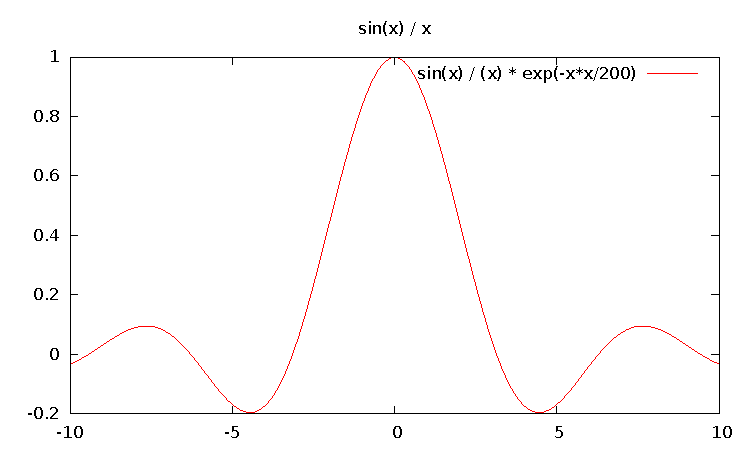
\includegraphics{Charts/pdf/PearsonRho.pdf}
	\caption{pdf of the Distribution of the Sample Correlation Coefficient}
	\label{Fig pdf of the Distribution of the Sample Correlation Coefficient}
\end{figure}



\subsection{Density and CDF}

\begin{mpFunctionsExtract}
	\mpFunctionFourNotImplemented
	{PearsonRhoDist? mpNumList? pdf, CDF and related information for the distribution of the sample correlation coefficient}
	{x? mpNum? A real number}
	{N? mpNum? A real number greater 2, representing the sample size}
	{rho? mpNum? A real number greater 0, representing the correlation coefficient}
	{Output? String? A string describing the output choices}
\end{mpFunctionsExtract}


\vspace{0.3cm}
See section \ref{Functions returning pdf, CDF, and related information} for the options for {\itshape\sffamily Output}. Algorithms and formulas are given in sections \ref{rhoDistributionDensity} and \ref{rhoDistributionCDF}.

\subsubsection{Density: Hotelling's algorithm}
\nomenclature{$f_R(r, N; \rho)$}{pdf of the Distribution of the Sample Correlation Coefficient}
\label{rhoDistributionDensity}

We define
\begin{equation}  \label{eq:PearsonRho_Def_ABCU}
	x = \rho r,\quad \quad  A=\sqrt{1-\rho^2}, \quad B=\sqrt{1-x^2}, \quad C=\sqrt{1-r^2}, \quad U=\frac{\arccos(-x)}{B}
\end{equation}
The probability density function for $R$ is then given by \citep{hotelling_1953}
\begin{equation} \label{eq:PearsonRho_PDF_Ik_def}
	f_R(r, N; \rho) = K_1 A^{N-1} C^{N-4} (1-x)^{\tfrac{3}{2}-N}{}_2F_1\left(\tfrac{1}{2},\tfrac{1}{2}; N-\tfrac{1}{2}; \tfrac{1}{2}+\tfrac{1}{2}x\right),
\end{equation}
\begin{equation}  \label{eq:PearsonRho_K1}
	\text{where}  \quad  K_1 = \frac{(N-2)\Gamma(N-1)}{\sqrt{2\pi}\Gamma\left(N-\tfrac{1}{2}\right)},  
\end{equation}
\begin{equation}  \label{eq:PearsonRho_T1}
	{}_2F_1\left(\tfrac{1}{2},\tfrac{1}{2}; N-\tfrac{1}{2}; \tfrac{1}{2}+\tfrac{1}{2}x\right) =  \sum_{i=0}^{\infty} M_i,
\end{equation}
\begin{equation} 
	M_0= 1, \quad M_i = M_{i-1} \frac{a_i^2}{c_i} \frac{1+x}{2i}
\end{equation}
$a_1=\tfrac{1}{2}$, $c_1 = N-\tfrac{1}{2}$, $a_i=a_{i-1}+1$, $c_i=c_{i-1}+1$ and ${}_2F_1(\cdot)$ is the Gaussian hypergeometric function (see section \ref{sec:Hypergeometric2F1MpMath}).


\subsubsection{Density :Closed form expressions and recursions}
For $N = 3,4$ the probability density function can be expressed in closed form \citep{odeh_1986}:
\begin{equation}  \label{eq:PearsonRho_Closed_f3_density}
	f_R(r, 3; \rho) = \frac{A^2(1+xU)}{\pi B^2C} 
\end{equation}
\begin{equation} \label{eq:PearsonRho_Closed_f4_density}
	f_R(r, 4; \rho) =\frac{AC^3 (B^2U + 3x(1+xU))}{\pi B^4} 
\end{equation}
where $x, A, B, C$ and $U$ are defined in  (\ref{eq:PearsonRho_Def_ABCU}). The probability density function $f_N(r,\rho)$ satisfies the following recurrence formula for $N \geq 5$ \citep{hotelling_1953}:
\begin{equation} \label{eq:PearsonRho_PDF_Ik_recur}
	f_R(r, N; \rho) = \frac{2N-5}{B^2(N-3)} x A C f_R(r, N-1; \rho) + \frac{N-3}{B^2(N-4)} A^2 C^2 f_R(r, N-2; \rho)  
\end{equation}
For $0 \leq x \leq 1$, eqn (\ref{eq:PearsonRho_PDF_Ik_recur}) can be used to find a sequence of values for $f_5(r;\rho), f_6(r;\rho),...,f_{N}(r;\rho)$. However, for $-1 < x < 0$ the recurrence formula is numerically unstable, since the two terms on the right-hand of eqn  are of opposite sign. In this case $(1+x)<1$, so the series given by eqn (\ref{eq:PearsonRho_PDF_Ik_def}) will converge extremely fast and can be used.



\subsubsection{CDF: Hotelling's series}
\label{rhoDistributionCDF}
\citet{hotelling_1953}  defines $Q_N(r;\rho) = \text{Pr}[\rho<R<r]$ and develops  $Q_N(r;\rho)$ in the following uniformly convergent series for $-1<\rho<r<1$. 

\begin{equation}
	Q_N(r,\rho) = K_1 \sum_{j=0}^{\infty}{\frac{(1 \cdot 3 \cdots (2j-1))^2 S_j}{j! 2^{2j} \cdot (2N+1) \cdots (2N+2j-1)}},
\end{equation}
where $K_1$ and $S_j$ are defined in equations (\ref{eq:PearsonRho_K1}) and (\ref{eq:PearsonRho_Hotelling_Sj}), respectively. From the relationships
\begin{equation}
	P_N(r, \rho) = 1-F_R(r, N; \rho) = Q_N(1,\rho)-Q_N(r,\rho)
\end{equation}
\begin{equation}
	P_N(-1, \rho) = 1
\end{equation}
\begin{equation}
	F_R(r, N; \rho) = 1 -P_N(r, \rho)
\end{equation}
\begin{equation}
	F_R(-r, N; -\rho) = 1 -F_R(r, N; \rho)
\end{equation}
we can compute $F_N(r;\rho)$ for any value of r and $\rho$ with $-1 \leq r \leq 1$, $-1<\rho<1$.
Hotelling shows that the error committed by truncating the series at any point is less than $\frac{2}{1-|\rho|}$ times the last term used. However, it is important to note that the series converges very slowly for small values of $N$, and in this case a large number of terms must be computed.

\begin{equation}  \label{eq:PearsonRho_Hotelling_Sj}
	S_j = \sum_{k=0}^{j} \binom{j}{k}(-1)^k \: \tfrac{1}{2} (1-\rho^2)^k \: 2^{j-k}  N_k
\end{equation}
\begin{equation}
	N_k = \sum_{s=0}^{\infty} \frac{\Gamma\left(\tfrac{3}{2}-k\right)}{\Gamma\left(\tfrac{3}{2}-k-s\right) s!} \cdot I \left(\tfrac{1}{2}(s+1), \tfrac{1}{2}(n-1),\frac{(r-\rho)^2}{(1-\rho r)^2}\right),
\end{equation} 
where $I(a,b;x)$ denotes the Incomplete Beta Function (see section \ref{sec:IncompleteBetaFunction}). Hotelling shows that in the evaluation of $N_k$ for large $s$ the absolute value of the ratio of the term of order $(s+1)$ to the term of order $s$ is bounded by $|\rho (r-\rho)/(1-\rho r)|$, so that the series converges rapidly.


\subsubsection{CDF: Guenther's series}
\citet{guenther_pearson_rho_1977} writes $P_N(r;\rho) = \text{Pr}[R>0] -  \text{Pr}[0<R<r]$ and develops $\text{Pr}[0<R<r]$ in an infinite series involving the Incomplete Beta Function denoted by $I(a,b;x)$. The result is
\begin{equation}  \label{eq:PearsonRho_Guenther_1}
	\text{Pr}[R>0] = \tfrac{1}{2} \left[1+\text{sgn}(\rho) \cdot I\left(\tfrac{1}{2}(N-1), \tfrac{1}{2}; \rho^2\right) \right]
\end{equation}
\begin{IEEEeqnarray}{rCl} \label{eq:PearsonRho_Guenther_2}
	\text{Pr}[0 < R <r] & = \sum_{j=0}^{\infty} K_1(j) \cdot I\left(\tfrac{1}{2}(N-2), \tfrac{1}{2}(2j+1); r^2 \right) \\
	& + \sum_{j=0}^{\infty} K_2(j) \cdot I\left(\tfrac{1}{2}(N-2), j+1; r^2 \right)  \nonumber
\end{IEEEeqnarray}

where  $K_1(j), K_2(j)$ are defined recursively by

\begin{equation*}
	K_1(0) = \tfrac{1}{2} \left(1-\rho^2 \right)^{\tfrac{1}{2}(N-1)}, \quad K_1(j)=\frac{2j+N-3}{2j} \rho^2 K_1(j-1)
\end{equation*}
\begin{equation*}
	K_2(0) = \frac{\Gamma \left(\tfrac{1}{2}N\right)}{\sqrt{\pi}\Gamma\left(\tfrac{1}{2}(N-1)\right)} \rho \left(1-\rho^2 \right)^{\tfrac{1}{2}(N-1)}, \quad K_2(j)=\frac{2j+N-2}{2j+1} \rho^2 K_2(j-1)
\end{equation*}\\
Eqns (\ref{eq:PearsonRho_Guenther_1}) and (\ref{eq:PearsonRho_Guenther_2}) are used together to give $P_N(r;\rho)$. Guenther also obtains error bounds for truncating the infinite series given by (\ref{eq:PearsonRho_Guenther_2}).


\subsubsection{CDF: Closed form expressions and recursions}

For $N = 3,4,5,6$ the cdf can be expressed in closed form \citep{odeh_1986}:
\begin{equation}  \label{eq:PearsonRho_Closed_F3}
	F_3(r; \rho) = \frac{\arccos(-r)}{\pi} - \frac{\rho C U}{\pi}
\end{equation}
\begin{equation} \label{eq:PearsonRho_Closed_F4}
	F_4(r; \rho) =\frac{\arccos(\rho)}{\pi} - \frac{\rho AC^2}{\pi B^2} - \frac{rA^3U}{\pi B^2}
\end{equation}
\begin{equation} \label{eq:PearsonRho_Closed_F5}
	F_5(r; \rho) =\frac{\arccos(-r)}{\pi} - \frac{(x^2-3\rho^3+2) r A^2C}{2\pi B^4} + \frac{(\rho^2-3+2\rho^2 x^2) \rho C^3U}{2\pi B^4} 
\end{equation}
\begin{IEEEeqnarray}{rCl} \label{eq:PearsonRho_Closed_F6}
	F_6(r; \rho) & = &\frac{\arccos(\rho)}{\pi} - \frac{[\rho r^2(2x^2+13) - 2\rho(4x^4+6x^2+5) + \rho^3(11x^2+4)] AC^2}{6\pi B^6} \\
	&& + \frac{2x^2(-2r^2+1)rA^5U}{6\pi B^6}  \nonumber
\end{IEEEeqnarray}
where $x, A, B, C$ and $U$ are defined in  (\ref{eq:PearsonRho_Def_ABCU}). The cumulative distribution function $F_N(r,\rho)$ satisfies the following recurrence formula  for $N \geq 7$\citep{hotelling_1953}:
\begin{IEEEeqnarray}{rCl}  \label{eq:PearsonRho_Closed_Recur}
	F_{N}(r;\rho) & = & \frac{2 (N - 4) \rho^2 - N + 5}{(N-3)\rho^2} F_{N-2}(r;\rho) \\
	&& +\: \frac{(N-5)A^2}{(N-3)\rho^2} F_{N-4}(r;\rho) \nonumber \\
	&& +\: \frac{(N-4)A^2C^2-(2N-9) B^2}{(N-4)(N-3)\rho^2 AC} \rho f_{N-1}(r;\rho)  \nonumber \\
	&& +\: \frac{(N-4)^2 +(3N(N-8)+47)\rho^2}{(N-4)^2 (N-3)\rho^2} r f_{N-2}(r;\rho)    \nonumber 
\end{IEEEeqnarray}
For $N$ odd, the above formula can be used repeatedly to find $F_7, F_9, ..., F_N$ starting with values of $F_3$ and $F_5$, for which exact expressions are given by eqns (\ref{eq:PearsonRho_Closed_F3}) and  (\ref{eq:PearsonRho_Closed_F5}) respectively. For $N$ even, the formula can be used repeatedly to find $F_8, F_{10}, ..., F_N$ starting with values of $F_4$ and $F_6$, for which exact expressions are given by equations (\ref{eq:PearsonRho_Closed_F4}) and (\ref{eq:PearsonRho_Closed_F6}) respectively.
However, the formula can only be applied if $\rho^2 \geq \frac{N-5}{2(N-4)}$, since if $\rho^2$ is less then this bound, the first two terms on the right hand side of eqn (\ref{eq:PearsonRho_Closed_Recur}) are of opposite sign and the formula is numerically unstable.


\subsubsection{CDF: Fisher's Approximation}
The widely used Fisher $z$-transformation leads to the approximation
\begin{equation}
	F_N(r,\rho) \approx \Phi \left( \sqrt{N-3} \left(Z(r) - Z(\rho) \right) \right), \quad \text{where} 
\end{equation}
$Z(\cdot)$ is defined in equation  (\ref{eq:PearsonRho_zTransform}), and $\Phi(\cdot)$ denotes the CDF of the normal distribution (see section \ref{sec:NormalDistribution_CDF}). This approximation can be improved by using the first 4 cumulants of $Z(R)$, resulting in
\begin{equation}
	F_N(r,\rho) \approx \Phi \left(x \right), \quad \text{where}
\end{equation}
\begin{equation}
	u= \frac{Z(r) - \kappa_1}{\sqrt{\kappa_2}}, \quad x = u + (u^2 - 1) \frac{\gamma_1}{6} + (u^3 - 3 u) \frac{\gamma_2}{24} + (4 u^3 - 7u) \frac{\gamma_1^2}{36} 
\end{equation}
and $\kappa_1$, $\kappa_2$, $\gamma_1$ and $\gamma_2$ are defined in equations  (\ref{eq:PearsonRho_kappa1}) to  (\ref{eq:PearsonRho_gamma1}).

%
%\subsubsection{Winterbottom's Approximation DH}
%Particularly accurate results have been found by inverting Winterbottom's approximation for the confidence limits of $\rho$, (see section \ref{sec:Winterbottom_Approximation}), giving the following approximation to the CDF:
%\begin{equation}
%F_N(r,\rho) \approx \Phi \left(\frac{k}{6} - \frac{2c}{k} - \frac{b}{3}\right), \quad \text{where} \quad m = N - 1,
%\end{equation}
%\begin{equation*}
%a = \frac{1}{12\sqrt{m^3}} + \frac{6 r^4 - 3r^2 + 2}{48\sqrt{m^5}}, \quad  b = \frac{-r3}{6 a m^2}, \quad s=\frac{1}{a\sqrt{m}} + \frac{1+r^2}{4a\sqrt{m^3}} + \frac{11 r^4 - 2r^2 + 1}{32a\sqrt{m^5}} 
%\end{equation*}
%\begin{equation*}
%t = \frac{Z(r)-Z(\rho)}{a} + \frac{r}{2 a m} + \frac{5 r^3 + 9r}{24 a m^2}, \quad d=t+ \frac{bs}{3} - \frac{2b^3}{27}
%\end{equation*}
%\begin{equation*}
%c = s-b^2/3, \quad p=\sqrt{|12c^3+81d^2|}, \quad k=(108d+12p)^{1/3}
%\end{equation*}
%$Z(\cdot)$ is defined in equation  (\ref{eq:PearsonRho_zTransform}), and $\Phi(\cdot)$ denotes the CDF of the normal distribution (see section \ref{sec:NormalDistribution_CDF}).
%





\subsubsection{CDF: Winterbottom's Approximation}
\label{sec:Winterbottom_Approximation_CDF}
The CDF approximation given by \citep{winterbottom_1980} is:
\begin{equation}
	F_N(r,\rho) \approx \Phi \left(\sqrt{m}Y \right), \quad \text{where} \quad m=N-1,
\end{equation}
\begin{IEEEeqnarray}{rCl}
	Y & = & - \frac{r}{2m} - \frac{3r+r^3}{12m^2} + \left( 1 - \frac{1+r^2}{4m} + \frac{3 - 11r^4}{96m^2} \right) w \\
	&& +\:  \frac{3r-4r^3}{24m} w^2 - \left( \frac{1}{12} - \frac{2 + 7r^2- 6r^4}{48m} \right) w^3 + \frac{3}{160} w^5,  \nonumber 
\end{IEEEeqnarray}
$w = Z(r)-Z(\rho)$  and $Z(\cdot)$ is defined in equation  (\ref{eq:PearsonRho_zTransform}).







\subsection{Quantiles}


\begin{mpFunctionsExtract}
	\mpFunctionFourNotImplemented
	{PearsonRhoDistInv? mpNumList? quantiles and related information for the distribution of the sample correlation coefficient}
	{Prob? mpNum? A real number between 0 and 1.}
	{N? mpNum? A real number greater 2, representing the sample size}
	{rho? mpNum? A real number greater 0, representing the correlation coefficient}
	{Output? String? A string describing the output choices}
\end{mpFunctionsExtract}


\vspace{0.3cm}
For a given value of $\alpha, N$ and $\rho$ a $100\alpha$ percentage point of $R$ is the unique value of $R$, say $r_\alpha$, which satisfies $F_N(r_\alpha; \rho) = \alpha$

Let $u_\alpha$ = $\Phi^{-1}(\alpha)$ be the lower $100\alpha$ percentage point of the standard normal distribution (see section \ref{sec:NormalDistribution_Quantiles}). Then an approximation to the $100\alpha$ percentage point $r_\alpha$ is obtained by

\begin{equation}
	r_\alpha \approx Z^{-1}\left(Z(\rho)+\frac{u_{\alpha}}{\sqrt{N-3}}\right).
\end{equation}
$Z(\cdot)$  and $Z^{-1}(\cdot)$ are defined in equations  (\ref{eq:PearsonRho_zTransform}) and  (\ref{eq:PearsonRho_Inverse_zTransform}). This approximation can be improved by using the first 4 cumulants of $Z(R)$, resulting in
\begin{equation}
	r_\alpha \approx Z^{-1}\left(\kappa_1+x \sqrt{\kappa_2}\right) \quad \text{where} 
\end{equation}
\begin{equation}
	x = u_\alpha + (u_\alpha^2 - 1) \frac{\gamma_1}{6} + (u_\alpha^3 - 3 u_\alpha) \frac{\gamma_2}{24} + (2 u_\alpha^3 - 5u_\alpha) \frac{\gamma_1^2}{36} 
\end{equation}
and $\kappa_1$, $\kappa_2$, $\gamma_1$ and $\gamma_2$ are defined in equations  (\ref{eq:PearsonRho_kappa1}) to  (\ref{eq:PearsonRho_gamma1}).



\subsubsection{Winterbottom's Quantile Approximation}
\label{sec:Winterbottom's Quantile Approximation}
An approximation to the $100\alpha$ percentage point $r_\alpha$ is obtained by \citep{winterbottom_1980}
\begin{equation}
	r_\alpha \approx Z^{-1}(y), \quad \text{where }
\end{equation}
\begin{IEEEeqnarray}{rCl}
	y & = & Z(\rho) + \frac{u_\alpha}{\sqrt{m}} + \frac{\rho}{2m} + \frac{u_\alpha^3+3(3-\rho^2)u_\alpha}{12\sqrt{m^3}} + \frac{4\rho^3 u_\alpha^2 + 15\rho-\rho^3}{24m^2} \\
	&& +\: \frac{u_\alpha^5+(-60\rho^4+30\rho^2+80)u_\alpha^3 + (45\rho^4-21\rho^2+375)u_\alpha}{480\sqrt{m^5}}   \nonumber  
\end{IEEEeqnarray}
$Z(\cdot)$  and $Z^{-1}(\cdot)$ are defined in equations  (\ref{eq:PearsonRho_zTransform}) and  (\ref{eq:PearsonRho_Inverse_zTransform}).





\subsection{Properties}
\label{rhoDistributionProperties}

\begin{mpFunctionsExtract}
	\mpFunctionThreeNotImplemented
	{PearsonRhoDistInfo? mpNumList? moments and related information for the distribution of the sample correlation coefficient}
	{N? mpNum? A real number greater 2, representing the sample size}
	{rho? mpNum? A real number greater 0, representing the correlation coefficient}
	{Output? String? A string describing the output choices}
\end{mpFunctionsExtract}

\vspace{0.3cm}

See section \ref{Functions returning moments and related information} for the options for {\itshape\sffamily Output}. Algorithms and formulas are given below.



\subsubsection{The moments of $R$}
The moments of $R$ are given by \cite{Anderson_book_2003}, p. 166:
\begin{equation}
	\mathbb{E}\left(R^{2h+1}\right) = \frac{(1-\rho^2)^{n/2}}{\sqrt{\pi} \Gamma(n/2)} \sum_{i=0}^{\infty} {\frac{(2\rho)^{2i+1}}{(2i+1)!} \frac{\Gamma^2[(n+1)/2+i] \Gamma(h+i+3/2)}{\Gamma(n/2 +h+i+1)}   }
\end{equation}
\begin{equation}
	\mathbb{E}\left(R^{2h}\right) = \frac{(1-\rho^2)^{n/2}}{\sqrt{\pi} \Gamma(n/2)} \sum_{i=0}^{\infty} {\frac{(2\rho)^{2i}}{(2i)!} \frac{\Gamma^2[(n+1)/2+i] \Gamma(h+i+1/2)}{\Gamma(n/2 +h+i)}   }
\end{equation}
The first 4 moments of the distribution of $R$ can also be expressed in terms of hypergeometric functions (see \cite{Johnson_1995} p.553):
%\begin{equation}
%\mu'_1= c_n \rho \times {}_2F_1\left(\tfrac{1}{2},\tfrac{1}{2};\tfrac{1}{2}(n+1);\rho^2 \right)
%\end{equation}
%\begin{equation}
%\mu'_2= 1 - \frac{(n-2)(1-\rho^2)}{n-1} \times {}_2F_1\left(1,1;\tfrac{1}{2}(n+1);\rho^2 \right)
%\end{equation}
%\begin{IEEEeqnarray}{rCl}
%\mu'_3 & = & c_n \left[ \rho \times {}_2F_1\left(\tfrac{1}{2},\tfrac{1}{2};\tfrac{1}{2}(n+1);\rho^2 \right) - \frac{(n-1)(n-2)}{\rho} \right] \\
%&& \times \: \left[{}_2F_1\left(\tfrac{1}{2},\tfrac{1}{2};\tfrac{1}{2}(n-1);\rho^2 \right) -  {}_2F_1\left(\tfrac{1}{2},\tfrac{1}{2};\tfrac{1}{2}(n+1);\rho^2 \right) \right] \nonumber  
%\end{IEEEeqnarray}
%\begin{IEEEeqnarray}{rCl}
%\mu'_4 & = &  1 + \frac{(n-2)(n-4)(1-\rho^2)}{2(n-1)} \times {}_2F_1\left(1,1;\tfrac{1}{2}(n+1);\rho^2 \right) \\
%&& - \:  \frac{n(n-2)(n-\rho^2)}{4\rho^2} \left[{}_2F_1\left(1,1;\tfrac{1}{2}(n+1);\rho^2 \right)-1\right] \nonumber  
%\end{IEEEeqnarray}

\begin{equation}
	\mu'_1 = c_n b_1 \rho
\end{equation}
\begin{equation}
	\mu'_2= 1 - \frac{b_2(n-2)(1-\rho^2)}{n-1}
\end{equation}
\begin{equation}
	\mu'_3= c_n  (b_3-b_1) \left(b_1 \rho - \frac{(n-1)(n-2)}{\rho} \right)
\end{equation}
\begin{equation}
	\mu'_4=  1 + \frac{b_2(n-2)(n-4)(1-\rho^2)}{2(n-1)} - \frac{(b_2 - 1)n(n-2)(n-\rho^2)}{4\rho^2} 
\end{equation}
with
\begin{equation}
	c_n = \frac{2}{n-1} \left[\frac{\Gamma(n/2)}{\Gamma((n-1)/2)}\right]^2
\end{equation}
\begin{equation}
	b_1 = {}_2F_1\left(\tfrac{1}{2},\tfrac{1}{2};\tfrac{1}{2}(n+1);\rho^2 \right)
\end{equation}
\begin{equation}
	b_2 = {}_2F_1\left(1,1;\tfrac{1}{2}(n+1);\rho^2 \right)
\end{equation}
\begin{equation}
	b_3 = {}_2F_1\left(\tfrac{1}{2},\tfrac{1}{2};\tfrac{1}{2}(n-1);\rho^2 \right)
\end{equation}
where $\Gamma(\cdot)$ is the Gamma function (see section \ref{GammaFunction}), and ${}_2F_1(\cdot)$ is the Gaussian hypergeometric function (see section \ref{sec:Hypergeometric2F1MpMath}).


\subsubsection{Fisher's z-transform}
The Fisher $z$-transform is defined by
\begin{equation}  \label{eq:PearsonRho_zTransform}
	Z(a)=\tfrac{1}{2} \log \left(\frac{1+a}{1-a}\right) = \text{atanh}(a)
\end{equation}

The inverse Fisher $z$-transform is defined by
\begin{equation} \label{eq:PearsonRho_Inverse_zTransform}
	Z^{-1}(a) = \frac{e^{2a}-1}{e^{2a}+1} = \tanh(a)
\end{equation}




\subsubsection{The cumulants of $Z(R)$}
Let $m = N - 1$. Then the first 4 cumulants of $Z(R)$ (with $Z(\cdot)$as defined in equation \ref{eq:PearsonRho_zTransform}) are given by \citep{hotelling_1953}
\begin{equation} \label{eq:PearsonRho_kappa1}
	\kappa_1= \tfrac{1}{2} \log \left(\frac{1+\rho}{1-\rho}\right) + \frac{\rho}{2m} + \frac{5+\rho^2}{4m^2} + \frac{11+2\rho^2+3\rho^4}{8m^3} + O(m^{-4})
\end{equation}
\begin{equation}
	\kappa_2=\frac{1}{m} + \frac{4-\rho^2}{2m^2} + \frac{22-6\rho^2-3\rho^4}{6m^3} + O(m^{-4})
\end{equation}
\begin{equation}
	\kappa_3=\frac{\rho^3}{m^3} + O(m^{-4})
\end{equation}
\begin{equation}
	\kappa_4=\frac{2}{m^3} + O(m^{-4})
\end{equation}
\begin{equation}  \label{eq:PearsonRho_gamma1}
	\gamma_1=\frac{\kappa_3}{\sqrt{\kappa_2}\kappa_2}, \quad \gamma_2=\frac{\kappa_4}{\kappa_2^2} 
\end{equation}



\subsection{Random Numbers}
\label{PearsonRhoDistributionRandom}

\begin{mpFunctionsExtract}
	\mpFunctionFiveNotImplemented
	{PearsonRhoDistRan? mpNumList? random numbers following the distribution of the sample correlation coefficient}
	{Size? mpNum? A positive integer up to $10^7$}
	{N? mpNum? A real number greater 2, representing the sample size}
	{rho? mpNum? A real number greater 0, representing the correlation coefficient}
	{Generator? String? A string describing the random generator}
	{Output? String? A string describing the output choices}
\end{mpFunctionsExtract}


\vspace{0.3cm}
See section \ref{Functions returning Random numbers} for the options for  {\itshape\sffamily Size},  {\itshape\sffamily Generator} and {\itshape\sffamily Output}. Algorithms and formulas are given below:


\vspace{0.3cm}
The correlation coefficient $r$ in samples of size $N>2$ from a non-singular bivariate normal population with correlation coefficent $\rho$ can be represented in the form
\begin{equation}
	\tilde{r} = \frac{z+ \tilde{\rho} \chi_{N-1}}{\chi_{N-2}}
\end{equation}
where $\tilde{r} =r/\sqrt{1-r^2}$ , $\tilde{\rho} =\rho/\sqrt{1-\rho^2}$, $z$ is a standardized normal variate and  $z$ , $\chi_{N-1}$, and $\chi_{N-2}$ are independent \citep{ruben_1966}. This can be used to develop an approximation where
\begin{equation}
	\frac{\sqrt{(2N-5)/2} \tilde{r} - \sqrt{(2N-3)/2} \tilde{\rho}}{\sqrt{1+ \tfrac{1}{2}( \tilde{r}^2+\tilde{\rho}^2)}}
\end{equation}
is distributed as a standard normal variate. See also \cite{akahira_1998}.







\subsection{Confidence limits for rho}
\label{PearsonRhoDistributionNC}


\begin{mpFunctionsExtract}
	\mpFunctionFourNotImplemented
	{PearsonRhoDistNoncentrality? mpNumList? confidence limits for the noncentrality parameter rhi and related information for the distribution of the sample correlation coefficient.}
	{alpha? mpNum? A real number between 0 and 1, specifies the confidence level (or Type I error).}
	{rho? mpNum? A real number between -1 and 1, representing the noncentrality parameter.}
	{N? mpNum? A real number greater 2, representing the sample size}
	{Output? String? A string describing the output choices}
\end{mpFunctionsExtract}


\vspace{0.3cm}
See section \ref{Functions related to noncentrality parameters} for the options for  {\itshape\sffamily alpha}, {\itshape\sffamily Noncentrality} and {\itshape\sffamily Output}. Algorithms and formulas are given below.

\vspace{0.3cm}
For a given value of $\alpha_1<\tfrac{1}{2}$, $N$, and an observed value of $R$, say $r_0$, a lower $100(1-\alpha_1)\%$ confidence limit on $\rho$ is the unique value of $\rho$, say $\rho_L$, which satisfies $F_N(r_0; \rho) = 1-\alpha_1$. A one-sided lower  $100(1-\alpha_1)\%$ confidence interval on $\rho$ is given by $\rho_L \leq \rho \leq 1$.

For $\alpha_1<\tfrac{1}{2}$, an upper $100(1-\alpha_2)\%$ confidence limit on $\rho$ is the unique value of $\rho$, say $\rho_U$, which satisfies $F_N(r_0; \rho) = 1-\alpha_2$. A one-sided upper $100(1-\alpha_2)\%$ confidence interval on $\rho$ is given by  $-1 \leq \rho \leq \rho_U$.

For $\alpha_1=1-\alpha_2=\alpha_0$, an equal-tailed two-sided  $100(1-2\alpha_0)\%$ confidence interval on $\rho$ is given by  $\rho_L \leq \rho \leq \rho_U$.


\subsubsection{Fisher's Approximation}
To obtain a confidence interval for ρ, we first compute a confidence interval for z(r). The inverse Fisher transformation bring the interval back to the correlation scale.
\begin{equation}
	\rho_L \approx Z^{-1}\left(Z(r)- \frac{u_{\alpha}}{\sqrt{N-3}}\right).
\end{equation}
For example, suppose we observe r = 0.3 with a sample size of n=50, and we wish to obtain a 95\% confidence interval for $\rho$. The transformed value is arctanh(0.3) = 0.30952, so the confidence interval on the transformed scale is $0.30952 - 1.96/\sqrt{47}$, or (0.023624, 0.595415). Converting back to the correlation scale yields (0.024, 0.534).

\subsubsection{Winterbottom's Approximation}
\label{sec:Winterbottom_Approximation}
Let $u_\alpha$ = $\Phi^{-1}(\alpha)$ be the lower $100\alpha$ percentage point of the standard normal distribution (see section \ref{sec:NormalDistribution_Quantiles}) and let $m=N-1$. Then an asymptotic approximation for a lower $100(1-\alpha)$ confidence limit on $\rho$ is given by \citep{winterbottom_1980}
\begin{equation}
	\rho_L \approx Z^{-1}(y), \quad \text{where }
\end{equation}
\begin{IEEEeqnarray}{rCl}
	y & = & Z(r) + \frac{u_\alpha}{\sqrt{m}} - \frac{r}{2m} + \frac{u_\alpha^3+3(1+r^2)u_\alpha}{12\sqrt{m^3}} - \frac{4r^3 u_\alpha^2 + 5r^3+9r}{24m^2} \\
	&& +\: \frac{u_\alpha^5+(60r^4-30r^2+20)u_\alpha^3 + (165r^4+30r^2+15)u_\alpha}{480\sqrt{m^5}}   \nonumber  
\end{IEEEeqnarray}
$Z(\cdot)$  and $Z^{-1}(\cdot)$ are defined in equations  (\ref{eq:PearsonRho_zTransform}) and  (\ref{eq:PearsonRho_Inverse_zTransform}).




\subsection{Sample Size Function}
\nomenclature{$N_{Rho}\left(\alpha, \beta, \widetilde{\rho} \right)$}{Sample size function of the noncentral $t$-distribution for a given confidence level $\alpha$, power $\beta$ and modified noncentrality parameter $\widetilde{\rho}$}
\label{PearsonRhoDistributionSampleSize}

\begin{mpFunctionsExtract}
	\mpFunctionFourNotImplemented
	{PearsonRhoDistSampleSize? mpNumList? sample size estimates and related information for the distribution of the sample correlation coefficient.}
	{alpha? mpNum? A real number between 0 and 1, specifies the confidence level (or Type I error).}
	{beta? mpNum?  A real number between 0 and 1, specifies the Type II error (or 1 - Power).}
	{ModifiedNoncentrality? mpNum? A real number greater 0, representing the modified noncentrality parameter.}
	{Output? String? A string describing the output choices}
\end{mpFunctionsExtract}

\vspace{0.3cm}
See section \ref{Functions returning Sample Size estimates} for the options for  {\itshape\sffamily alpha}, {\itshape\sffamily beta}, {\itshape\sffamily ModifiedNoncentrality} and {\itshape\sffamily Output}. Algorithms and formulas are given below.

\vspace{0.3cm}
We denote by $N_{Rho}\left(\alpha, \beta, \widetilde{\rho} \right)$  the sample size function of the noncentral $t$-distribution for a given confidence level $\alpha$, power $\beta$ and modified noncentrality parameter $\widetilde{\rho}$. This function determines the minimal sample size $N$ for given noncentrality parameter, Type I error $1-\alpha$, and Type II error $1-\beta$, where  $\delta = \sqrt{N}\widetilde{\rho}$ 





\newpage
\section{Distribution of the Sample Multiple Correlation Coefficient}
\label{Rho2Distribution}



\subsection{Definition}
\label{Rho2DistributionDefinition}

Let $(X_1, \ldots, X_N)$ be a sample of independent vector observations from a  $p$-variate normal population with mean $\boldsymbol{\mu}$ and covariance matrix $\boldsymbol{\Sigma}$. Define
\begin{equation}
	\overline{X} = \frac{1}{N} \sum_{i=1}^N X_i \quad and \quad \textbf{A} = \sum_{i=1}^N (X_i - \overline{X}) (X_i - \overline{X})'.
\end{equation}
Partition $\textbf{A}$ as
\begin{equation}
	\textbf{A} =
	\begin{pmatrix}
		a_{11} & \textbf{a}_{12} \\
		\textbf{a}_{21} & \textbf{A}_{22} 
	\end{pmatrix}
\end{equation}
so that $a_{11}$ is $1 \times 1$, $\textbf{a}_{12}$ is $1 \times (p-1)$, and $\textbf{A}_{22}$ is a $(p-1) \times (p-1)$ matrix. In terms of these submatrices, the squared sample multiple correlation coefficient is given by

\begin{equation}
	R^2 = \frac{\textbf{a}_{12} \textbf{A}_{22}^{-1} \textbf{a}_{21}}{a_{11}}
\end{equation}
The sample multiple correlation coefficient is the positive square root of $R^2$. The squared population multiple correlation coefficient, $\rho^2$, is defined similarly in terms of the submatrices of $\boldsymbol{\Sigma}$.

For given $N-p \geq 1$, the distribution of $R^2$ is independent of $\boldsymbol{\mu}$ and $\boldsymbol{\Sigma}$, but depends upon  $\rho^2$, where $0 \leq \rho^2 < 1$.
For $0 \leq x \leq 1$, define $f_{R^2}(x;p,N,\rho^2)$ to be the probability density function for $R^2$. We denote the cumulative distribution function of $R^2$ by

\begin{equation}
	F_{R^2}(x;p,N,\rho^2) = \text{Pr}[R^2 \leq x] = \int_{0}^{x}{f_{R^2}(t;p,N,\rho^2)) dt}.
\end{equation}


Note: The univariate version of the noncentral distribution of Wilks $\Lambda$: Canonical Correlation 
(see section \ref{WilksLambdaDistributionDefinition_CORR})
is equivalent to $W=1-R^2$.




\subsection{Density and CDF}

\begin{mpFunctionsExtract}
	\mpFunctionFiveNotImplemented
	{Rho2Dist? mpNumList? pdf, CDF and related information for the distribution of the squared population multiple correlation coefficient}
	{x? mpNum? A real number}
	{p? mpNum? An integer greater 2, representing the number of variates}
	{N? mpNum? A real number greater p, representing the sample size}
	{Rho2? mpNum? A real number greater or equal 0, representing the squared sample multiple correlation coefficient}
	{Output? String? A string describing the output choices}
\end{mpFunctionsExtract}



\subsubsection{Density: Infinite series}
\nomenclature{$f_{R^2}(x;p,n,\rho^2)$}{pdf of the Square of the Multiple Sample Correlation Coefficient}
\label{Rho2DistributionDensity}

The density function of the multiple sample correlation coefficient is given by \citep{Ding_1996,Benton_2003}
\begin{equation}
	f_{R^2}(x;p,N,\rho^2) = \sum_{i=0}^\infty f_{\text{NegBin}}\left((N-1)/2, i; 1-\rho^2\right) \times f_{\text{Beta}}\left(x; \tfrac{1}{2}(p-1) + i, \tfrac{1}{2}(N-p)\right)
\end{equation}
where $f_{\text{NegBin}}(\cdot)$ denotes the pmf of the negative binomial distribution (see section \ref{NegativBinomialDistributionDensity}) and $f_{\text{Beta}}(\cdot)$ denotes the pdf of the Beta distribution (see section \ref{BetaDistributionDensity})


\subsubsection{Density: Representation in terms of hypergeometric functions}
The density function of the multiple sample correlation coefficient is given by \citep{lee_results_1971,gurland_1968}
\begin{equation}
	f_{R^2}(x;p,n,\rho^2) = \frac{(1-\rho^2)^{n/2} (x)^{(n_1-2)/2} (1-x)^{(n_2-2)/2} {}_2F_1(\tfrac{1}{2}n, \tfrac{1}{2}n, \tfrac{1}{2}n_1; \rho^2 x)}{B(\tfrac{1}{2}n_1,\tfrac{1}{2}n_2 )}
\end{equation}

\begin{equation}
	f_{R^2}(x;p,N,\rho^2) = f_{Beta}\left(x; \tfrac{1}{2}(p-1), \tfrac{1}{2}(N-p)\right) (1-\rho^2)^{n/2} \times {}_2F_1(\tfrac{1}{2}N, \tfrac{1}{2}N, \tfrac{1}{2}p; \rho^2 x)
\end{equation}
where $f_{\text{Beta}}(\cdot)$ denotes the pdf of the Beta distribution (see section \ref{BetaDistributionDensity}) 
and ${}_2F_1(\cdot)$ is the Gaussian hypergeometric function (see section \ref{sec:Hypergeometric2F1MpMath}).

\subsubsection{Density: Closed form expressions for odd $p$}
For the particular cases of $p=3$ and $p=5$, we have for the pdf \citep{lee_results_1971}:
\begin{equation}
	f_{R^2}(n,3;\rho^2)  = \frac{ (n-3)\sqrt{1-\rho^2} \left[f_{R}(n-1,R;\rho) - f_{R}(n-1,-R;\rho)\right] }{2(n-2)\rho\sqrt{1-R^2}}
\end{equation}

\begin{IEEEeqnarray}{rCl} 
	f_{R^2}(n,5;\rho^2) & = & \frac{ (n-5)(1-\rho^2)R \left[f_{R}(n-2,R;\rho) + f_{R}(n-2,-R;\rho)\right]}{2(n-2)\rho^2(1-R^2)} \\
	& - & \frac{2(1-\rho^2)(1-R^2) f_{R^2}(n-2,3;\rho^2)}{2(n-2)\rho^2(1-R^2)}  \nonumber
\end{IEEEeqnarray}
where $f_{R}(\cdot)$ denotes the pdf of the distribution of the sample correlation coeffcient (see section \ref{rhoDistributionDensity}).
Starting with these formulas, the pdf can be calculated for all odd $p$, using the recurrence relation given in equation (\ref{eq:RecurrenceR2pdf}).




\subsubsection{CDF: Infinite series}
\nomenclature{$F_{R^2}(x;p,n,\rho^2)$}{CDF of the Square of the Multiple Sample Correlation Coefficient}
The CDF of the multiple sample correlation coefficient is given by \citep{Ding_1996,Benton_2003}
\begin{equation}
	F_{R^2}(x;p,N,\rho^2) = \sum_{i=0}^\infty f_{\text{NegBin}}\left((N-1)/2, i; 1-\rho^2\right) \times  F_{\text{Beta}}\left(x; \tfrac{1}{2}(p-1) + i, \tfrac{1}{2}(N-p)\right)
\end{equation}
where $f_{\text{NegBin}}(\cdot)$ denotes the pmf of the negative binomial distribution and $F_{\text{Beta}}(\cdot)$ denotes the CDF of the Beta distribution (see section \ref{BetaDistributionCDF})
where $f_{\text{NegBin}}(\cdot)$ denotes the pmf of the negative binomial distribution (see section \ref{NegativBinomialDistributionDensity}) and $F_{\text{Beta}}(\cdot)$ denotes the CDF of the Beta distribution (see section \ref{BetaDistributionCDF})


\subsubsection{CDF: Series of Gurland}
Let $R^2$ be the sample multiple correlation coefficent between $X$ (consisting of $p-1$ variates) and $Y$, based on $N$ observations. If both $X$ and $Y$ are random variates, then 
distribution of $F$ is given by \citep{lee_tables_1972,Gurland_1970}, 
\begin{equation}
	\text{Pr}[F \leq x] = F_{R^2}(x;a,b,\rho^2) = \frac{b^m}{a^{n/2}}  \sum_{j=0}^{\infty}{c_j I(m+j,k,y)} \quad \text{where}
\end{equation}
\begin{equation*}
	z=F(p-1), \quad y=\frac{z}{z+(N-p)}, \quad a=\frac{1}{1-\rho^2}, \quad n=(N-p)/2, \quad m=(p-1)/2
\end{equation*}
\begin{equation*}
	c_0=1, \quad c_j=\frac{c_{j-1}(-n/2-j+1)\rho^2}{j}
\end{equation*}


\subsubsection{CDF: Closed form expressions for odd $p$}
For the particular cases of $p=3$ and $p=5$, we have for the CDF \citep{lee_results_1971}:
\begin{equation}
	F_{R^2}(n,3;\rho^2) = F_{R^2}(n,1;\rho^2) - \frac{\sqrt{(1-\rho^2)(1-R^2)}\left[f_{R}(n-1,R;\rho) - f_{R}(n-1,-R;\rho)\right] }{(n-2)\rho}
\end{equation}

\begin{IEEEeqnarray}{rCl} 
	F_{R^2}(n,5;\rho^2) &=& F_{R^2}(n,3;\rho^2) - \frac{(1-\rho^2)R \left[f_{R}(n-2,R;\rho) - f_{R}(n-2,-R;\rho)\right] }{(n-2)\rho} \quad \quad \\
	& - & \frac{(1-\rho^2) \left[F_{R^2}(n-2,3;\rho^2) - F_{R^2}(n-2,1;\rho^2) \right]}{(n-2)\rho}  \nonumber
\end{IEEEeqnarray}
where $F_{R}(\cdot)$ denotes the CDF of the distribution of the sample correlation coeffcient (see section \ref{rhoDistributionCDF}).
Starting with these formulas, the CDF can be calculated for all odd $p$, using the recurrence relation given in equation (\ref{eq:RecurrenceR2CDF}).


\subsubsection{CDF: Approximation by non-central F}
\cite{lee_results_1971} suggests the following approximation, based on the noncentral $F$ distribution:
\begin{equation}
	F_{R^2}(x;n_1,n_2,\rho^2) \thickapprox F_{F'}\left(y; \nu, n_2, \lambda\right), \quad \text{where}
\end{equation}
\begin{center}
	
	$\gamma=1/(1-\rho^2)$, 
	
	\vspace{0.3cm}
	$A_j=(n_1+n_2) (\gamma^{\:j}-1) + n_1, \quad j=1,2,3, $
	
	\vspace{0.3cm}
	$G = (A_2 - \sqrt{A_2^2  -A_1 A_3})/A_1$, 
	
	\vspace{0.3cm}
	$\lambda=\rho^2 \gamma \sqrt{\gamma (n_1+n_2) n_2}/G^2 $,
	
	\vspace{0.3cm}
	$\nu= (A_2/G^2)- 2\lambda$, 
	
	\vspace{0.3cm}
	$y= x/(1-x) \times n_2/(\nu \cdot G)$, 
	
\end{center}

and $F_{F'}\left(\cdot; \nu, n_2, \lambda\right)$ denotes the CDF of the noncentral $F$ distribution with $\nu$ and $n_2$ degrees of freedom and noncentrality parameter $\lambda$ 
%(see section \ref{NoncentralFDistributionCDFBoost})
. For performance reasons, the noncentral $F$ distribution is evaluated using the (fast and highly accurate) saddlepoint approximation given in section \ref{NoncentralFDistributionCDFSaddlepoint}, rather than any of the "exact" algorithms.




\subsubsection{CDF: 2-moment approximation by central F}
\begin{equation}
	F_{F'}(x;n_1,n_2,\rho^2)  \thickapprox  F_F\left(x/c; m_1, n_2\right), 
\end{equation}
where $c=A_1/n_1$, $m_1= A_1^2/A_2$, $A_1=(n_1+n_2) (\gamma-1)+n_1$, $A_2=(n_1+n_2) (\gamma^2-1)+n_1$, $\gamma=1/(1-\rho^2)$, and $F_F\left(\cdot; m_1, n_2\right)$ denotes the CDF of a central $F$ distribution with $m_1$ and $n_2$ degrees of freedom (see \ref{FDistributionCDF}.






\subsection{Quantiles}

\begin{mpFunctionsExtract}
	\mpFunctionFiveNotImplemented
	{Rho2DistInv? mpNumList? quantiles and related information for the distribution of the squared population multiple correlation coefficient}
	{Prob? mpNum? A real number between 0 and 1.}
	{p? mpNum? An integer greater 2, representing the number of variates}
	{N? mpNum? A real number greater p, representing the sample size}
	{Rho2? mpNum? A real number greater or equal 0, representing the squared sample multiple correlation coefficient}
	{Output? String? A string describing the output choices}
\end{mpFunctionsExtract}

See section \ref{Functions returning Quantiles} for the options for  {\itshape\sffamily Prob} and {\itshape\sffamily Output}). Algorithms and formulas are given below.



\vspace{0.3cm}
An approximation to $Rho^2_{\alpha,n_1,n_2,\lambda} $, the $\alpha$-quantile of the distribution of the squared population multiple correlation coefficient with $p$ variates, sample size $N$ the distribution of the squared population multiple correlation coefficient and noncentrality parameter $\rho^2$, is obtained as
\begin{equation}
	F_{\alpha,n_1,n_2,\lambda}  \thickapprox  c \cdot F_{\alpha,m_1,n_2,} 
\end{equation}
where $c=A_1/n_1$, $m_1= A_1^2/A_2$, $A_1=(n_1+n_2) (\gamma-1)$, $A_2=(n_1+n_2) (\gamma^2-1)$, $\gamma=1/(1-\rho^2)$, and $F_{\alpha,m_1,n_2}$ denotes the $\alpha$-quantile of a central $F$-distribution with $m_1$ and $n_2$ degress of freedom (see section \ref{FINV}). 




\subsection{Properties}
\label{Rho2DistributionProperties}

\begin{mpFunctionsExtract}
	\mpFunctionFourNotImplemented
	{Rho2DistInfo? mpNumList? moments and related information for the distribution of the squared population multiple correlation coefficient}
	{p? mpNum? An integer greater 2, representing the number of variates}
	{N? mpNum? A real number greater p, representing the sample size}
	{Rho2? mpNum? A real number greater or equal 0, representing the squared sample multiple correlation coefficient}
	{Output? String? A string describing the output choices}
\end{mpFunctionsExtract}

\vspace{0.3cm}

See section \ref{Functions returning moments and related information} for the options for {\itshape\sffamily Output}. Algorithms and formulas are given below.



\subsubsection{Recurrence relations}
\cite{lee_results_1971} gives the following recurrence relations for the pdf and CDF, valid for all integer values of $p \geq 6$:
\begin{IEEEeqnarray}{rCl} \label{eq:RecurrenceR2pdf}
	(n-2)\rho^2(1-R^2) f_{R^2}(n,p;\rho^2) & = & (n-p)R^2(1-\rho^2) f_{R^2}(n-2,p-4;\rho^2) \\
	& - &  (p-4)(1-\rho^2)(1-R^2)  f_{R^2}(n-2,p-2;\rho^2)  \nonumber
\end{IEEEeqnarray}
\begin{IEEEeqnarray}{rCl} \label{eq:RecurrenceR2CDF}
	(n-2)\rho^2(1-R^2) F_{R^2}(n,p;\rho^2) & = & (n-p)\rho^2 F_{R^2}(n,p-2;\rho^2) \\
	& - &  (p-4)(1-\rho^2) \left[F_{R^2}(n-2,p-2;\rho^2) - F_{R^2}(n-2,p-4;\rho^2) \nonumber  \right]\\
	& - &  2R^2(1-\rho^2) f_{R^2}(n-2,p-4;\rho^2)  \nonumber
\end{IEEEeqnarray}


\subsubsection{The moments of $R^2$}
\label{MomentsR2}
\cite{Muirhead_1982}, p. 178, gives the following formula (see also \cite{Johnson_1995}, p. 621)
\begin{equation}
	\mathbb{E}[(1-R^2)^h] = \frac{\left[\tfrac{1}{2}(n-m+1)\right]_h}{\left(\tfrac{1}{2}n\right)_h} (1-\bar{R}^2)^h \times {}_2F_1(h,h,\tfrac{1}{2}n+h;\bar{R}^2).
\end{equation}
where $(a)_k$ is the Pochammer symbol (see section \ref{PochhammerSymbol}) and ${}_2F_1(\cdot)$ is the Gaussian hypergeometric function (see section \ref{sec:Hypergeometric2F1MpMath}).


The lower order moments are given by
\begin{equation}
	\mu'_1 = 1 - \frac{(n-m+1)}{n} (1-\bar{R}^2)^h \times {}_2F_1(1,1,\tfrac{1}{2}n+1;\bar{R}^2).
\end{equation}
\begin{equation}
	\mathbb{E}[(1-R^2)^2] = \frac{\left[\tfrac{1}{2}(n-m+1)\right]_2}{\left(\tfrac{1}{2}n\right)_2} (1-\bar{R}^2)^2 \times {}_2F_1(2,2,\tfrac{1}{2}n+2;\bar{R}^2).
\end{equation}







\subsection{Random Numbers}

\begin{mpFunctionsExtract}
	\mpFunctionSixNotImplemented
	{Rho2DistRan? mpNumList? random numbers following the distribution of the squared population multiple correlation coefficient}
	{Size? mpNum? A positive integer up to $10^7$}
	{p? mpNum? An integer greater 2, representing the number of variates}
	{N? mpNum? A real number greater p, representing the sample size}
	{Rho2? mpNum? A real number greater or equal 0, representing the squared sample multiple correlation coefficient}
	{Generator? String? A string describing the random generator}
	{Output? String? A string describing the output choices}
\end{mpFunctionsExtract}


\vspace{0.3cm}


A notable result concerning the distribution of $R^2$ is that $\tilde{R}^2 = R^2/(1-R^2)$ has the representation
\begin{equation}
	\tilde{R}^2 = \frac{(\tilde{\rho}\chi_n + z)^2 + \chi_{p-1}^2}{\chi_{n-p}^2} \label{eq:Rho2DistRandom}
\end{equation}
where $\tilde{\rho}^2 = \rho^2/(1-\rho^2)$, $n$ is the sample size less one, $z$ is a standard normal variate, $\chi_f$ and $\chi_f^2$ are chi and chi-square variates on $f$ degrees of freedem; 
the variates figuring in this relation are independently distributed and $\tilde{\rho}$ is taken to be positive \cite{lee_results_1971}.





\subsection{Confidence Limits for the Noncentrality Parameter}
\label{Rho2Noncentrality}

\begin{mpFunctionsExtract}
	\mpFunctionFiveNotImplemented
	{Rho2DistNoncentrality? mpNumList? confidence limits for the noncentrality parameter $\rho^2$ and related information for the distribution of the squared population multiple correlation coefficient.}
	{alpha? mpNum? A real number between 0 and 1, specifies the confidence level (or Type I error).}
	{Rho2? mpNum? A real number greater or equal 0, representing the squared sample multiple correlation coefficient}
	{p? mpNum? An integer greater 2, representing the number of variates}
	{N? mpNum? A real number greater p, representing the sample size}
	{Output? String? A string describing the output choices}
\end{mpFunctionsExtract}


\vspace{0.3cm}
See section \ref{Functions related to noncentrality parameters} for the options for  {\itshape\sffamily alpha}, {\itshape\sffamily Noncentrality} and {\itshape\sffamily Output}. Algorithms and formulas are given below.

\vspace{0.3cm}
Let $T$ be a statistic according to the non-central $t$-distribution
with $n$ degrees of freedom and a non-centrality parameter $\delta$. Then
the lower confidence limit $\widehat{\delta}$ of level $1-\alpha$ and the two-sided confidence interval $[ \underline{\delta},\overline{\delta}]$ of the
non-centrality parameter $\delta$ of level $1-\alpha$ are given by \cite{akahira_1995}:
\begin{equation}
	\widehat{\delta} = bT - z_\alpha \sqrt{k} +  h T^3 (z_\alpha^2 - 1)/k,
\end{equation} 
\begin{equation}
	\underline{\delta} = bT - z_{\alpha/2} \sqrt{k} +  h T^3 (z_{\alpha/2}^2 - 1)/k,
\end{equation} 
\begin{equation}
	\overline{\delta} = bT + z_{\alpha/2} \sqrt{k} -  h T^3 (z_{\alpha/2}^2 - 1)/k,
\end{equation} 
where $k=1+(1-b^2)T^2$, $h$ and $b$ are defined in equation (\ref{Akahira_h_b}), and $z_\alpha$ denotes the $\alpha$-quantile of the normal distribution (see section \ref{sec:NormalDistribution_Quantiles}).



\subsection{Sample Size}
\label{Rho2DistributionSampleSize}


\begin{mpFunctionsExtract}
	\mpFunctionFiveNotImplemented
	{Rho2DistSampleSize? mpNumList? sample size estimates and related information for for the distribution of the squared population multiple correlation coefficient}
	{alpha? mpNum? A real number between 0 and 1, specifies the confidence level (or Type I error).}
	{beta? mpNum?  A real number between 0 and 1, specifies the Type II error (or 1 - Power).}
	{p? mpNum? An integer greater 2, representing the number of variates}
	{ModifiedNoncentrality? mpNum? A real number greater 0, representing the modified noncentrality parameter.}
	{Output? String? A string describing the output choices}
\end{mpFunctionsExtract}


\vspace{0.3cm}
See section \ref{Functions returning Sample Size estimates} for the options for  {\itshape\sffamily alpha}, {\itshape\sffamily beta}, {\itshape\sffamily ModifiedNoncentrality} and {\itshape\sffamily Output}. Algorithms and formulas are given below.




\newpage
\section{Skew Normal Distribution}

\subsection{Definition}
\label{SkewNormalDistributionDefinition}

In probability theory and statistics, the skew normal distribution is a continuous probability distribution that generalises the normal distribution to allow for non-zero skewness.

See also \href{http://en.wikipedia.org/wiki/Skew_normal_distribution}{http://en.wikipedia.org/wiki/Skew\_normal\_distribution}. 


\subsection{Density and CDF}

\begin{mpFunctionsExtract}
	\mpFunctionFiveNotImplemented
	{SkewNormalDistBoost? mpNumList? returns pdf, CDF and related information for the skew normal distribution}
	{x? mpNum? A real number.}
	{a? mpNum? The location parameter.}
	{b? mpNum? The scale parameter}
	{c? mpNum? The shape parameter}
	{Output? String? A string describing the output choices}
\end{mpFunctionsExtract}


\vspace{0.3cm}
See section \ref{Functions returning pdf, CDF, and related information} for the options for {\itshape\sffamily Output}. Algorithms and formulas are given in sections \ref{SkewNormalDistributionDensity} and \ref{SkewNormalDistributionCDF}.




\subsubsection{Density}
\label{SkewNormalDistributionDensity}

%The probability density function with location parameter $\xi$, scale parameter $\omega$, and shape parameter $\alpha$  is
%\begin{equation} 
%f(\xi;\omega,\alpha)= \frac{2}{\omega} \phi \left(\frac{x-\xi}{\omega}\right)  \Phi \left(\alpha \left(\frac{x-\xi}{\omega}\right)\right)  
%\end{equation}

The probability density function with location parameter $a$, scale parameter $b$, and shape parameter $c$  is
\begin{equation} 
f(x;a,b,c)= \frac{2}{b} \phi \left(\frac{x-a}{b}\right)  \Phi \left(c \left(\frac{x-a}{b}\right)\right)  
\end{equation}


\subsubsection{CDF}
\label{SkewNormalDistributionCDF}

%\begin{equation} 
%F(\xi;\omega,\alpha)=  \Phi \left(\frac{x-\xi}{\omega}\right) -  2T \left(\frac{x-\xi}{\omega}, \alpha \right)
%\end{equation}

\begin{equation} 
F(a,b,c)=  \Phi \left(\frac{x-a}{b}\right) -  2T \left(\frac{x-a}{b}, c \right)
\end{equation}

where  $T_{\text{Owen}}(\cdot,\cdot)$ denotes Owen's $T$ function (see section \ref{sec:OwenTFunction}).

\subsection{Quantiles}
\label{SkewNormalDistributionQuantiles}



\begin{mpFunctionsExtract}
	\mpFunctionFiveNotImplemented
	{SkewNormalDistInvBoost? mpNumList? returns quantiles and related information for the the skew normal distribution}
	{Prob? mpNum? A real number between 0 and 1.}
	{a? mpNum? The location parameter.}
	{b? mpNum? The scale parameter}
	{c? mpNum? The shape parameter}
	{Output? String? A string describing the output choices}
\end{mpFunctionsExtract}

\vspace{0.3cm}
See section \ref{Functions returning Quantiles} for the options for  {\itshape\sffamily Prob} and {\itshape\sffamily Output}). 
The quantile is determined using an iterative alogorithm.


\subsection{Properties}
\label{SkewNormalDistributionProperties}


\begin{mpFunctionsExtract}
	\mpFunctionFourNotImplemented
	{SkewNormalDistInfoBoost? mpNumList? returns moments and related information for the skew normal distribution}
	{a? mpNum? The location parameter.}
	{b? mpNum? The scale parameter}
	{c? mpNum? The shape parameter}
	{Output? String? A string describing the output choices}
\end{mpFunctionsExtract}

\vspace{0.3cm}

See section \ref{Functions returning moments and related information} for the options for {\itshape\sffamily Output}. Algorithms and formulas are given below.

\subsubsection{Moments}

\begin{equation} 
\mu_1 = a+bd\sqrt{\frac{2}{\pi}}, \quad \text{where } d=\frac{c}{\sqrt{1+c^2}}
\end{equation}

\begin{equation} 
\mu_2 = b^2 \left(1-\frac{2d^2}{\pi} \right)
\end{equation}

\begin{equation} 
\gamma_1 = \frac{4-\pi}{2} \frac{\left(d\sqrt{2/\pi}\right)^3}{(1-2d^2/\pi)^{3/2}}
\end{equation}

\begin{equation} 
\gamma_2 = 2(\pi-3) \frac{\left(d\sqrt{2/\pi}\right)^4}{(1-2d^2/\pi)^{2}}
\end{equation}


\subsection{Random Numbers}
\label{SkewNormalDistributionRandom}

\begin{mpFunctionsExtract}
	\mpFunctionSixNotImplemented
	{SkewNormalDistRanBoost? mpNumList? returns random numbers following a skew normal distribution}
	{Size? mpNum? A positive integer up to $10^7$}
	{a? mpNum? The location parameter.}
	{b? mpNum? The scale parameter}
	{c? mpNum? The shape parameter}
	{Generator? String? A string describing the random generator}
	{Output? String? A string describing the output choices}
\end{mpFunctionsExtract}

\vspace{0.3cm}

See section \ref{Functions returning Random numbers} for the options for  {\itshape\sffamily Size},  {\itshape\sffamily Generator} and {\itshape\sffamily Output}. 
%Algorithms and formulas are given below.


\subsection{Owen's T-Function}
\label{sec:OwenTFunction}
\nomenclature{$T_{\text{Owen}}(a,b)$}{Owen's T-Function}


\begin{mpFunctionsExtract}
	\mpFunctionTwo
	{TOwenBoost? mpNum? Owen's T-Function}
	{h? mpNum? A real number.}
	{a? mpNum? A real number.}
\end{mpFunctionsExtract}

\vspace{0.3cm}
Owen's T-Function is defined as \citep{owen_1956}:

\begin{equation}
	T(h,a) = \frac{1}{2\pi} \int_0^a \frac{\exp \left[-\tfrac{1}{2} h^2 (1+x^2)\right]}{1+x^2} dx
\end{equation}

The implementation uses the algorithm descibed in \cite{patefield_2000}.





\newpage
\section{Multivariate Normal Distribution}


\subsection{Definition}
\label{MultivariateNormalDistributionDefinition}
An $n$-dimensional random variable $\textbf{X}$ with mean vector $\boldsymbol{\mu}$ and covariance matrix  $\boldsymbol{\Sigma}$ is said to have a nonsingular multivariate normal distribution, in symbols $\boldsymbol{X}  \sim \mathcal{N}_n(\boldsymbol{\mu}, \boldsymbol{\Sigma})$, if  $\boldsymbol{\Sigma}$ is positive definite, and the density function of $\textbf{X}$ is of the form given in equation \ref{eq:MultivariateNormalDistributionDensity}.

See also \cite{Steck_1962}and \cite{owen_moments_1962}

See \cite{Lai_2006}

\subsection{Density of the  multivariate normal distribution}
\label{MultivariateNormalDistributionDensity}

The density of the  multivariate normal distribution is given by \citep{Tong_1990}:
\begin{equation} \label{eq:MultivariateNormalDistributionDensity}
	f(\boldsymbol{x; \mu, \Sigma}) = \frac{1}{(2\pi)^{n/2}  \vert \boldsymbol{\Sigma} \vert ^{1/2}} e^{-Q_n(\boldsymbol{x; \mu, \Sigma})/2}, \quad \boldsymbol{x} \in \Re^n
\end{equation}
where
\begin{equation}
	Q_n(\boldsymbol{x; \mu, \Sigma}) = (\boldsymbol{x - \mu})' \boldsymbol{\Sigma^{-1}} (\boldsymbol{x - \mu}).
\end{equation}




\subsection{Bivariate Normal}

The bivariate normal distribution has the following density:
\begin{equation}
	g(x,y;\rho) = \frac{1}{2 \pi \sqrt{1-\rho^2}} e^{\frac{-(x^2 -2\rho x y + y^2)}{2(1-\rho^2)}}
\end{equation}


The method develped by \cite{owen_1956} was for a long time the most widely used approach to calculate bivariate normal (BVN) probabilities. Owen showed that

\begin{equation}
	\Phi_2(-\infty, b1,b2;\rho) = \frac{\Phi(b_1) - \Phi(b_2)}{2} - T_{\text{Owen}}(b_1,\widehat{b_1}) - T_{\text{Owen}}(b_2,\widehat{b_2}) - c, 
\end{equation}

where $\rho$ is the correlation coefficient,  $T_{\text{Owen}}(\cdot,\cdot)$ denotes Owen's $T$ function (see section \ref{sec:OwenTFunction}), and


\begin{equation}
	c=\begin{cases}
		0, &  \text{if }b_1 b_2 > 0 \text{ or }b_1 b_2 = 0,  b_1 + b_2 \geq 0\\
		\frac{1}{2} & \text{otherwise, }
	\end{cases}
\end{equation}

\begin{equation}
	\widehat{b_1} = \frac{b_2 - b_1 \rho}{b_1 \sqrt{1-\rho^2}}, \quad \widehat{b_2} = \frac{b_2 - b_2 \rho}{b_2 \sqrt{1-\rho^2}}.
\end{equation}


\vspace{0.3cm}
\cite{abramowitz_handbook_1970} gives the following representation:

\begin{equation}
	B(h,k;\rho) = \int_{-\infty}^k {\int_{-\infty}^h} g(x,y;\rho) dx dy
\end{equation}

\begin{equation}
	L(h,k;\rho) = \int_{k}^\infty {\int_{h}^\infty} g(x,y;\rho) dx dy
\end{equation}

\begin{equation}
	L(-h,-k;\rho) = B(h,k;\rho) 
\end{equation}

Integral epresentation \cite{Tong_1990}:
\begin{equation}
	B(h,k;\rho) = \int_{-\infty}^\infty {\prod_{j=1}^2} \left(\frac{d_j \sqrt{\vert \rho \vert} z + a_j} {\sqrt{1-\rho}} \right) \phi(z) dz
\end{equation}

where $d_j=-1$ if $\rho<0$ and $j=2$ and $d_j=1$ otherwise.


\subsection{Special structure: zero correlation}
This case covers the normal maximum 

\begin{equation}
	F_{MM}(x,k,\mu) = \prod_{i=1}^k \left[\Phi(x-\mu_i)\right]
\end{equation}

\begin{equation}
	F_{M}(x,k) = \left[\Phi(x)\right]^k
\end{equation}


This case covers the normal maximum modulus

\begin{equation}
	F_{MM}(x,k,\mu) = \prod_{i=1}^k \left[\Phi(x-\mu_i) - \Phi(-x-\mu_i)\right]
\end{equation}


\begin{equation}
	F_{MM}(x,k,0) = \left[\Phi(x) - \Phi(-x)\right]^k = \left[2\Phi(x) - 1\right]^k, \quad x>0
\end{equation}


See \cite{Stoline_1979}

See \cite{Narula_1978}



\subsection{Special structure: Equal-correlated case}
With $\rho_{ij}=\rho$, we have for a one-sided test \cite{Tong_1990}:

\begin{equation}
	F_n(h;\rho) = \int_{-\infty}^\infty \left[\Phi \left(\frac{h + \sqrt{\vert \rho \vert} y} {\sqrt{1-\rho}} \right) \right]^n \phi(y) dy =  \int_{-\infty}^\infty \cdots  \int_{-\infty}^\infty g(h;\rho) dx_1 \cdots dx_n.
\end{equation}

and for a two-sided test:

\begin{equation}
	F_n(h;\rho) = \int_{-\infty}^\infty \left[\Phi \left(\frac{h + \sqrt{\vert \rho \vert} y} {\sqrt{1-\rho}} \right) - \Phi \left(\frac{-h + \sqrt{\vert \rho \vert} y} {\sqrt{1-\rho}} \right) \right]^n \phi(y) dy =  \int_{-h}^\infty \cdots  \int_{-h}^\infty g(h;\rho) dx_1 \cdots dx_n.
\end{equation}


Note: The distribution of the twosided version can get bi-modal for large arguments, if $P(x)$ is calculated. This requires modification of the search algorithm.


\subsection{Special structure: Dunnett test}


See \cite{dunnett_multiple_1955}

See also \cite{Cheng_1995}

For $\lambda_i$ = $\sqrt{\rho} \geq 0$ for all $i$, this reduces to the equicorrelated case. 

With $\rho_{ij}=\lambda_i  \lambda_j$, we have for a one-sided test:

\begin{equation}
	F_n(h;\rho_{ij}) = \int_{-\infty}^\infty \prod_{i=1}^n  \left[\Phi \left(\frac{(a_i-\mu_i)/\sigma_i + \lambda_i z} {\sqrt{1-\lambda_i^2}} \right) \right] \phi(y) dz
\end{equation}

and for a two-sided test:

\begin{equation}
	F_n(h;\rho_{ij}) = \int_{-\infty}^\infty \prod_{i=1}^n  \left[\Phi \left(\frac{(a_i-\mu_i)/\sigma_i + \lambda_i z} {\sqrt{1-\lambda_i^2}} \right) - \Phi \left(\frac{(b_i-\mu_i)/\sigma_i + \lambda_i z} {\sqrt{1-\lambda_i^2}} \right) \right] \phi(y) dz
\end{equation}


Note: The distribution of the twosided version can get bi-modal for large arguments, if $P(x)$ is calculated. This requires modification of the search algorithm.


\subsection{Special structure: normal range}
%\subsection{Definition}
%\label{StudentizedRangeDistributionDefinition}

Let $X_1, \dots, X_k$ be a random sample of size $k$ from a  $N(\mu, \sigma^2)$ distribution. Let $s^2$ be an independent mean square estimate of $\sigma^2$ with $n$ degrees of freedom.

Then $Q_n = \text{max} \vert X_i - X_j \vert, 1<i<j<k$, has a Normal Range distribution with $k$ degrees of freedom, and 
$Q_t = Q_n / s$ has a Studentized Range distribution with $k$ and $n$ degrees of freedom \cite{Hochberg_1987}.

See also \cite{Stoline_1978} and \cite{Harter_1960} and \cite{David_1972}

\subsubsection{Density}
\label{NormalRangeDistributionDensity}

The density in the central case is given by

\begin{equation}
	p(x) = k(k-1)  \int_{-\infty}^\infty \left( \Phi(y) - \Phi(y-x) \right)^{k-2} \phi(y) \phi(y-x) dy
\end{equation}

%
%\subsection{CDF}
%\begin{tabular}{p{481pt}}
%\toprule
%\textsf{Function \textbf{StudentizedRangeDist}($\boldsymbol{a}\ As\ mpNum$, $\boldsymbol{b}\ As\ mpNum$) As mpNum}\index{Multiprecision Functions!StudentizedRangeDist} \\
%\bottomrule
%\end{tabular}
%
%\vspace{0.3cm}
%\lipsum[2]
\subsubsection{Normal Range}

\begin{equation}
	Q(x) = \sum_{i=1}^k  \int_{-\infty}^\infty \phi(y_i - \mu_i) \left( \prod_{i=1, j \neq i}^k (\Phi(y_i - \mu_i) - \Phi(y_i - \mu_i -x) \right) dy_i
\end{equation}
for $\mu=0$ this simplifies to

\begin{equation}
	Q(x) = k  \int_{-\infty}^\infty \phi(y) \left( \Phi(y) - \Phi(y-x) \right)^{k-1} dy
\end{equation}

\begin{equation}
	P(x) = 1 - Q(x) = k  \int_{-\infty}^\infty \phi(y) \left( L_1^k - [L_1 - L_2]^{k-1} \right) dy, \quad \text{where}
\end{equation}
\begin{equation}
	L_1 = \Phi(y), \quad L_2 = \Phi(y-x), \quad L_2 \rightarrow 0 \text{ for } x \rightarrow \infty
\end{equation}
\begin{equation}
	L_1^k - (L_1 - L_2)^k = L_1^k \left( 1 - \left( 1 - \frac{L_2}{L_1} \right) ^k \right) 
\end{equation}





\subsection{Normal Orthant Probabilities}
\label{NormalOrthantProbabilities}
Let $X=(X_1, X_2, \cdots , X_n)$  be a random vector distributed as $N(0,R_n)$ , where $R_n$ is positive definite. The normal orthant probability is defined as
\begin{equation}
	P_n = \int_0^\infty N(0,R_n) d^n x.
\end{equation}
Based on the method of \cite{Sun_1988_Therory, Sun_1988_Computation}, this probability can be expressed as
\begin{equation}
	P_{2k}=  \frac{1}{2^{2k}} + \frac{1}{2^{2k-1}\pi} \sum_{i<j=1}^{2k}{\arcsin(r_{ij})} + \sum_{j=2}^{k}{\frac{1}{2^{2k-j}\pi^j}}   \sum_{i_1<i_2<\cdots<i_{2j}}^{2k}{I_{2j}(R^{(i_1i_2\cdots i_{2j})})},    
\end{equation}
\begin{equation}
	P_{2k+1}=  \frac{1}{2^{2k+1}} + \frac{1}{2^{2k}\pi} \sum_{i<j=1}^{2k+1}{\arcsin(r_{ij})} + \sum_{j=2}^{k}{\frac{1}{2^{2k+1-j}\pi^j}}   \sum_{i_1<i_2<\cdots<i_{2j}}^{2k+1}{I_{2j}(R^{(i_1i_2\cdots i_{2j})})},    
\end{equation}
where $R^{(i_1i_2\cdots i_{2j}})$ denotes the submatrix consisting of the $(i_1i_2\cdots i_{2j})^{th}$ rows and columns of $R_n$,
\begin{equation}
	I_n(\Lambda_n) = (-2\pi)^{-k}  \int_{-\infty}^\infty \prod_{i=1}^n \frac{1}{\omega_i} \exp(-\tfrac{1}{2} \omega^t \Lambda_n \omega) d^n \omega, \quad n=2k,
\end{equation}
and $\Lambda_n=(\lambda_{ij})$ is a covariance matrix of n variates.

See \cite{Genz_2002, Genz_2009} for alternative methods

\subsection{Normal Rank Order Probabilities}
Consider the situation where random variables $X_1,\ldots,X_m$ and $X_1,\ldots,Y_n$ are normally distributed with means $\mu_X$ and $\mu_Y$, respectively, and common variance $\sigma^2$, all $m+n$ random variables being mutually independent and $d=(\mu_Y - \mu_X)/\sigma$. 

Let $\textbf{U} = (U_1,\ldots,U_{m+n}), U_1 < \cdots < U_{m+n}$, denote the order statistics of the random variables $ (X_1,\ldots,X_{m}), (Y_1,\ldots,Y_{n})$, and let $\textbf{Z} = (Z_1,\ldots,Z_{m+n})$ denote a random vector of zeros and ones, where the $i$th component $\textbf{Z}_i$ is 0 (or 1) if $U_i$ is an $X$ (or $Y$). Denote by $\phi(x-\theta)$ the normal density with mean $\theta$ and variance 1 (see section \ref{sec:NormalDistribution_pdf}). If  $\textbf{z} = (z_1,\ldots,z_{m+n})$ is a fixed vector of zeros and ones, the probability of the rank order $z$, Pr$[\textbf{Z}=\textbf{z}]$, is given by

\begin{equation} \label{eq:MiltonIntegral}
	P_{m.n}(\textbf{z} \vert d) = m!n! \idotsint\limits_R \prod_{i=1}^{m+n} \phi(t_i - z_i d) dt_i,
\end{equation}
where the region of integration $R$ is $-\infty < t_1 \leq t_2  \leq \cdots  \leq t_{m+n} < \infty$. \cite{Milton_1970} describes a $p$-dimensional midpoint algorithm that economizes the number of arithmetic operations required to evaluate equation (\ref{eq:MiltonIntegral}), corrects for effects of the edges of the region of integration and involves no high-degree quadrature formulas.






\subsection{Random Numbers}

\subsubsection{Generation of Exchangeable Normal Variates}
\label{Generation of Exchangeable Normal Variates}
Consider the situation in which we are interested in generating $N$ (pseudo) independent $n$-dimensional variates $\textbf{X}_1,\ldots, \textbf{X}_N$, such that $\textbf{X} = (X_{1t},\ldots,X_{nt})' (t=1,\ldots,N)$ has an $\mathcal{N}_n(\boldsymbol{\mu}, \boldsymbol{\Sigma})$ distribution with a common mean $\mu$, a common variance $\sigma^2$, and a common correlation coefficient $\rho \in [0,1)$. Then a corresponding algorithm for generating $\textbf{X}_1,\ldots, \textbf{X}_N$ is:

Input $\mu, \sigma^2, \rho, n$, and $N$.

For $t=1,\ldots,N$ compute
\begin{equation} 
	X_{it} = \mu + \sigma \left(\sqrt{1-\rho} Z_{it} + \sqrt{\rho} Z_{0t}  \right) \label{eq:normalrand1}
\end{equation}
and form $\textbf{X} = (X_{1t},\ldots,X_{nt})'$.


\subsubsection{Generation of Multivariate Normal Variates with a Special Correlation Structure}
In certain statistical applications the covariance matrix $\boldsymbol{\Sigma} = (\sigma_{ij})$ may be of the form

\begin{equation}
	\sigma_{ij}=\begin{cases}
		\sigma_{i} & \text{for }i=j\\
		\sigma_{i} \sigma_{j} \lambda_{i} \lambda_{j}  & \text{for }i \neq j,
	\end{cases}
\end{equation}

where $\lambda_i \in [-1, 1] (i=1,\ldots,n)$. In this case, the correlation coefficients are $\rho_{ij} = \lambda_i \lambda_j$ for all $i \neq j$. To generate $\textbf{X}_1,\ldots, \textbf{X}_N$ according to an  $\mathcal{N}_n(\boldsymbol{\mu}, \boldsymbol{\Sigma})$ distribution when $\boldsymbol{\Sigma}$ has such a structure and $\boldsymbol{\mu} =(\mu_1,\ldots,\mu_n)'$, we replace equation \ref{eq:normalrand1} by
\begin{equation} 
	X_{it} = \mu_i + \sigma_i \left(\sqrt{1-\lambda_i^2} Z_{it} + \lambda_i Z_{0t}  \right) 
\end{equation}
and otherwise follow the algorithm in section \ref{Generation of Exchangeable Normal Variates}. Note that here the $\mu_i$ are not necessarily the same and the correlation coefficients are not necessarily all nonnegative. If $\mu_i=\mu$, $\sigma_i=\sigma$, and $\lambda_i=\sqrt{\rho} \geq 0 (i=1,\ldots,n)$, then this algorithm reduces to the one in section \ref{Generation of Exchangeable Normal Variates} as a special case.


\subsubsection{Generation of Multivariate Normal Variates with an Arbitrary Nonsingular Multivariate Normal Distribution}

We are interested in generating $\textbf{X}_1,\ldots, \textbf{X}_N$ from an  $\mathcal{N}_n(\boldsymbol{\mu}, \boldsymbol{\Sigma})$ distribution with arbitrary but fixed $\boldsymbol{\mu}$ and $\boldsymbol{\Sigma}$ (which is positive definite).

Let $\textbf{T} = (\tau_{ij})$ be the unique lower triangular $n \times n$ matrix (obtained by Cholesky decomposition) such that $\textbf{TT'} = \boldsymbol{\Sigma}$.
If  $\textbf{Z} \sim \mathcal{N}_n(\boldsymbol{0}, \boldsymbol{I_n})$, then $\textbf{X} = \textbf{TZ} + \boldsymbol{\mu}$ has an  $\mathcal{N}_n(\boldsymbol{\mu}, \boldsymbol{\Sigma})$ distribution. 

Consequently, to generate independent random variates $\textbf{X}_1,\ldots, \textbf{X}_N$ according to this distribution, the following algorithm may be used:


\vpara
Compute $\textbf{T} = (\tau_{ij})$

Input $N, n, \boldsymbol{\mu} =(\mu_1,\ldots,\mu_n)'$ and  $\textbf{T} = (\tau_{ij})$.

Generate $Z_{1t}, \ldots, Z_{nt}$ (which are (pseudo) independent $\mathcal{N}(0,1)$ variates) and apply the transformation $\textbf{X}_t = \textbf{TZ}_t + $ $\boldsymbol{\mu}$, i.e. compute

\begin{equation} 
	X_{it} = \sum_{j=1}^i \tau_{ij} Z_j + \mu_i, \quad \text{for } i=1,\ldots,n,
\end{equation}
and then form $\textbf{X} = (X_{1t},\ldots,X_{nt})'$.

Repeat this step for $t=1,\ldots,N$.




\newpage
\section{Multivariate t-Distribution}


\subsection{Definition}
\label{MultivariateTDistributionDefinition}
Let $\boldsymbol{R} = (\rho_{ij})$ be an $n \times n$ symmetric matrix such that it is either positive definite or positive semidefinite and $\rho_{ii} = 1 (i=1,\ldots,n)$.
Let  $\textbf{Z} = (Z_1,\ldots,Z_{n})'$ have an $\mathcal{N}_n(\boldsymbol{0}, \boldsymbol{R})$ distribution, and let the univariate variable $S$ be such that $S$ is independent of $\boldsymbol{Z}$, and $\nu S^2$ has a $\chi^2(\nu)$ distribution. Then a natural generalization of the Student's $t$ variable is

\begin{equation}
	\boldsymbol{t} = (t_1,\ldots,t_n)' = \left(\frac{Z_1}{S},\ldots,\frac{Z_n}{S}\right)' .
\end{equation}




If $\boldsymbol{R}$ is positive definite, then the density of $\boldsymbol{t}$ (with correlation matrix $\boldsymbol{R}$ and degrees of freedom $\nu$) is given by \citep{Tong_1990}:

\begin{equation}
	h(\boldsymbol{t; R}, \nu)= \frac{\Gamma((n+\nu)/2)}{(\nu \pi)^{n/2} \Gamma(\nu/2) \vert \boldsymbol{R}  \vert^{1/2}} \left(1+\frac{1}{\nu} \boldsymbol{t}' \boldsymbol{R}^{-1} \boldsymbol{t} \right)^{-(n+\nu)/2} , \quad \boldsymbol{t} \in \Re^n.
\end{equation}



\subsection{Studentized Maximum and Maximum Modulus}

\begin{equation}
	\frac{\partial}{\partial c} \left(F(c x) g(x)\right) = x g(x) F'(c x)
\end{equation}



\subsubsection{Density and CDF}
Let $X_1,\ldots,X_k$ be a random sample of size $k$ from a $\mathcal{N}(0,\sigma^2)$ distribution. Let $s^2$ be an independent mean square estimate of $\sigma$ with $n$ degrees of freedom. Then 

\begin{equation}
	Q=\frac{\text{max}X_j}{s}, \quad j=1,\ldots,k
\end{equation}
has a Studentized Maximum distribution with $k$ and $n$ degrees of freedom, and

\begin{equation}
	Q=\frac{\text{max}|X_j|}{s}, \quad j=1,\ldots,k
\end{equation}
has a Studentized Maximum Modulus distribution with $k$ and $n$ degrees of freedom.




\subsubsection{Quantiles}

Studentized  Maximum  Critical  Values  $M_{k, \nu, \alpha}$   (One-sided  Multivariate  $t$  Critical  Values  $t_{k, \nu, \rho=0 , \alpha}$) 

Studentized Maximum Modulus Critical Values $|M|_{k, \nu, \alpha}$   (Two-sided 
Multivariate  $t$  Critical  Values  $|t|_{k, \nu, \rho=0 , \alpha}$) 







\subsection{Dunnett's t}

\subsubsection{Density and CDF}
Let $X_1,\ldots,X_k$ be a random sample of size $k$ from a $\mathcal{N}(0,\sigma^2)$ distribution. Let $s^2$ be an independent mean square estimate of $\sigma$ with $n$ degrees of freedom. Then 

\begin{equation}
	Q=\frac{\text{max}X_1 - X_j}{s}, \quad 1<j<k
\end{equation}
has a onesided Dunnett's $t$-distribution with $k$ and $n$ degrees of freedom, and

\begin{equation}
	Q=\frac{\text{max}|X_1 - X_j|}{s}, \quad 1<j<k
\end{equation}
has a twosided Dunnett's $|t|$-distribution with $k$ and $n$ degrees of freedom.


For Dunnett's test:
\begin{equation}
	\lambda_i=\frac{1}{\sqrt{1+n_0/n_i}}
\end{equation}


\subsubsection{Quantiles}

One-Sided  Multivariate  t  Critical Values $t_{k, \nu, \rho=\lambda_i \lambda_j , \alpha}$   Common  Correlation  $\rho=0.5$ 


Two-Sided  Multivariate  t  Critical Values $|t|_{k, \nu, \rho=\lambda_i \lambda_j  , \alpha}$   Common  Correlation  $\rho=0.5$ 



\subsection{Studentized Range}

Let $X_1,\ldots,X_k$ be a random sample of size $k$ from a $\mathcal{N}(0,\sigma^2)$ distribution. Let $s^2$ be an independent mean square estimate of $\sigma$ with $n$ degrees of freedom. Then 

\begin{equation}
	Q=\frac{\text{max}|X_i - X_j|}{s}, \quad 1<i<j<k
\end{equation}
has a Studentized Range distribution with $k$ and $n$ degrees of freedom.

\subsubsection{Density and CDF}

\begin{equation}
	Q_t(c; n) =  \int_{0}^\infty Q_n(cx) g(x, n) dx, \quad \text{where}
\end{equation}
\begin{equation}
	g(x; n) =  \frac{n^{n/2}}{2^{(n-1)/2} \Gamma(n/2)}x^{n-1}e^{-nx^2 /2} \quad \text{is the pdf of } \frac{s}{\sigma}
\end{equation}

\begin{equation}
	SR(c) =   \int_{0}^\infty Q(cx) g(x) dx, \text{ and for } n=\infty, \quad SR(c)=Q(c).
\end{equation}


\subsubsection{Quantiles}

Critical  Values $q_{k, \nu, \alpha}$   for  the  Studentized  Range  Distribution 



See \cite{Hirotsu_1979}





\subsection{Special case Owen}
Owen considers a special case of the bivariate noncentral t-distribution which is relevant in quality control \cite{owen_special_1965}



\newpage
\section{Noncentral Chi-Square Distribution}
\label{NoncentralChiSquareDistributionEx}


\subsection{Definition}

%\subsubsection{Noncentral Chi-Square Distribution}
\label{NoncentralChiSquareDistributionDefinitionEx}

Let $X_1, X_2, \ldots, X_n$ be independent and identically distributed random variables each following a normal distribution with mean $\mu_j$ and unit variance. 
Then $\chi^2 = \sum_{j=1}^n X_j$ is said to follow a noncentral $\chi^2$-distribution with $n$ degress of freedom and noncentrality parameter \mbox{$\lambda = \sum_{j=1}^n (\mu_j - \mu)$.} 




\subsection{Density and CDF}

\begin{mpFunctionsExtract}
	\mpFunctionFourNotImplemented
	{NoncentralCDistEx? mpNumList? pdf, CDF and related information for the noncentral $\chi^2$-distribution}
	{x? mpNum? A real number}
	{n? mpNum? A real number greater 0, representing the degrees of freedom}
	{lambda? mpNum? A real number greater 0, representing the noncentrality parameter}
	{Output? String? A string describing the output choices}
\end{mpFunctionsExtract}


\vspace{0.3cm}
See section \ref{Functions returning pdf, CDF, and related information} for the options for {\itshape\sffamily Output}. Algorithms and formulas are given in sections \ref{NoncentralChiSquareDistributionDensityEx} and \ref{NoncentralChiSquareDistributionCDFEx}.




\label{NoncentralChiSquareDistributionDensityEx}
\nomenclature{$f_{\chi^2}(n, x; \lambda)$}{pdf of the noncentral chi-square distribution}

\subsubsection{Density: Closed form representations}
The density of a noncentral chi-square variable with $n$ degrees of freedom  and $\lambda$ is given by  \citep{Wang1993}
\begin{equation}
	f_{\chi^2}\left(n, x; \lambda\right) =  e^{-\lambda/2} f_{\chi^2}(n, x)  {}_0F_1 \left(-; \frac{n}{2}; \frac{x \lambda}{4}\right)
\end{equation}
\begin{equation}
	f_{\chi^2}\left(n, x; \lambda\right) = \tfrac{1}{2} e^{-(\lambda+x)/2} \left( \frac{x}{\lambda}\right)^{(n-2)/2}  I_{(n-2)/2}\left(\sqrt{\lambda x}\right)
\end{equation}

where $f_{\chi^2}(n, \cdot)$ is the pdf of the (central) $\chi^2$ distribution (see section \ref{ChiSquareDistributionDensity}, ${}_0F_1(\cdot)$ is the  confluent hypergeometric limit function (see section \ref{Hypergeometric0F1MpMath}), and $I_{\nu}(\cdot)$ is the modified Bessel function of the first kind of order $\nu$ (see section  \ref{BESSELInu}).


\subsubsection{Density and CDF: Finite series for odd degrees of freedom}
For odd degrees of freedom, the pdf and cdf can be expressed as a finite sum, using the recurrence relations given in section \ref{NoncentralChiSquareDistributionRecur}, and defining $h(n,x,\lambda) = e^{(1/2)(x+\lambda)} f_{\chi^2}\left(n, x; \lambda\right)$ \citep{Andras_2008}:
\begin{equation}
	F_{\chi^2}\left(1, x;\delta^2 \right) = \Phi(x-\delta)-\Phi(-x-\delta)
\end{equation}
\begin{equation}
	h(1, x;\lambda)   = \frac{\cosh (\sqrt{x\lambda})}{\sqrt{2\pi x}}, \quad h(3, x;\lambda)   = \frac{\sinh (\sqrt{x\lambda})}{\sqrt{2\pi \lambda}}
\end{equation}
where  $\Phi(\cdot)$ denotes the cdf of the normal distribution (see section \ref{sec:NormalDistribution_CDF}).


\subsubsection{CDF: General formulas}
\label{NoncentralChiSquareDistributionCDFEx}
\nomenclature{$F_{\chi^2}(n, x; \lambda)$}{CDF of the noncentral chi-square distribution}

The cdf of a noncentral chi-square variable with $n$ degrees of freedom and $\lambda$ is given by
\begin{equation}
	\text{Pr}\left[\chi^2 \le x\right] = F_{\chi^2}\left(n, x; \lambda\right) =  \int_{0}^{x} f_{\chi^2}\left(n, t; \lambda\right) dt
\end{equation} 

\subsubsection{CDF: Infinite series in terms of the central cdf}
The cdf of a noncentral chi-square variable with $n$ degrees of freedom and $\lambda$ is given by
\begin{equation}
	F_{\chi^2}\left(n, x; \lambda\right) = e^{-\lambda/2} \sum_{j=0}^\infty {\frac{(\lambda /2)^j}{j!} F_{\chi^2}\left(n+2+j, x\right) }
\end{equation} 
where $F_{\chi^2}(n, \cdot)$ is the cdf of the (central) $\chi^2$ distribution (see section \ref{sec:ChiSquareDistribution_cdf}).

\subsubsection{CDF: Infinite series in terms of the central pdf}
\cite{ding_1992} gives the following representation (this is used by Boost for small lambda):
\begin{equation}
	F_{\chi^2}\left(n, x; \lambda\right) = 2e^{-\lambda/2} \sum_{i=0}^\infty f_{\chi^2}\left(n+2+2i, x\right) \left(\sum_{k=0}^i{\frac{(\lambda /2)^k}{k!}}\right)
\end{equation} 
where $f_{\chi^2}(n, \cdot)$ is the pdf of the (central) $\chi^2$ distribution (see section \ref{ChiSquareDistributionDensity}).




\subsubsection{CDF: Integral representation}
\cite{Chou_1985} gives the following representation for $n \geq 2$ and $\lambda \geq 0$:
\begin{equation}
	F_{\chi^2}\left(n, x; \lambda\right) = \frac{2^{(1-n)/2}\sqrt{2\pi}}{ \Gamma((n-1)/2))}  \int_{0}^{x} y^{(n-3)/2} \phi \left(\sqrt{y}\right) \left[\Phi \left(\sqrt{x-y}-\sqrt{\lambda}\right) - \Phi \left(-\sqrt{x-y}-\sqrt{\lambda}\right) \right]dy
\end{equation} 
where $\phi(\cdot)$ denotes the pdf of the normal distribution (see section \ref{sec:NormalDistribution_pdf}) and  $\Phi(\cdot)$ denotes the cdf of the normal distribution (see section \ref{sec:NormalDistribution_CDF}).

\subsubsection{CDF: 2 moment approximation}
\cite{Patnaik_1949} gives the following 2-moment approximation based on the central $\chi^2$-distribution:
\begin{equation}
	F_{\chi^2}\left(n, x; \lambda\right) \thickapprox F_{\chi^2}\left(n_1, x_1;\right), \quad \text{where } n_1= \frac{(n+\lambda)^2}{n+2\lambda} , \quad  x_1= \frac{x(n+\lambda)}{n+2\lambda}
\end{equation} 
where $F_{\chi^2}(n, \cdot)$ is the cdf of the (central) $\chi^2$ distribution (see section \ref{sec:ChiSquareDistribution_cdf}).




\subsubsection{CDF: 3 moment approximation}
\cite{Pearson_1959} gives the following 3-moment approximation based on the central $\chi^2$-distribution:
\begin{equation}
	F_{\chi^2}\left(n, x; \lambda\right) \thickapprox F_{\chi^2}\left(n_1, x_1;\right), \quad \text{where } n_1= \frac{(n+2\lambda)^3}{2(n+3\lambda)^2}, \quad  x_1= \frac{x+\lambda^2/(n+3\lambda)}{2(n+3\lambda)/n+2\lambda}
\end{equation} 
where $F_{\chi^2}(n, \cdot)$ is the cdf of the (central) $\chi^2$ distribution (see section \ref{sec:ChiSquareDistribution_cdf}).


\subsubsection{CDF: Saddlepoint approximation}
\cite{Butler_2007} suggests the following approximation:
\begin{equation}
	K(t) = - \frac{n}{2} \log(1-2t) + \frac{\lambda t}{1-2t}, \quad t \in \left(-\infty, \tfrac{1}{2}\right)
\end{equation}

\begin{equation}
	K^{(j)}(t) = \frac{2^{j-1}(j-1)!}{(1-2t)^j} \left[n + \frac{\lambda j}{1-2t}   \right]
\end{equation}

\begin{equation}
	s(x)=-\frac{1}{4x} \left[n-2x+\sqrt{n^2+4x\lambda} \right], \quad x>0
\end{equation}



\subsubsection{CDF: Wiener Germ approximation}
\cite{Penev_2000} give the following first and second order Wiener germ approximation:
\begin{equation}
	F_{\chi^2}\left(n, x; \lambda\right) \thickapprox \Phi \left(\text{sgn}(s) \sqrt{n(s-1)^2(1/(2s) + m- h(1-s)/s) - \ln(A(s)) + 2B(s)/n} \right)
\end{equation} 
\begin{equation}
	\text{where } m = \lambda/n; \quad h(y) = \frac{(1-y) \ln(1-y)+y- \tfrac{1}{2}y^2}{y^2} ; \quad s= \frac{\sqrt{1+4xm/n}-1}{2m} 
\end{equation} 
\begin{equation}
	A(s) = \frac{1}{s} - \frac{2}{s} \cdot  \frac{h(1-s)}{1+2ms}; \quad  B(s) = \frac{(1+3m)^2}{9(1+2m)^3}
\end{equation} 
where  $\Phi(\cdot)$ denotes the cdf of the normal distribution (see section \ref{sec:NormalDistribution_CDF}).


\subsection{Quantiles}
\label{NoncentralChiSquareDistributionQuantilesEx}

\begin{mpFunctionsExtract}
	\mpFunctionFourNotImplemented
	{NoncentralCDistInvEx? mpNumList? quantiles and related information for the noncentral $\chi^2$-distribution}
	{Prob? mpNum? A real number between 0 and 1.}
	{n? mpNum? A real number greater 0, representing the degrees of freedom}
	{lambda? mpNum? A real number greater 0, representing the noncentrality parameter}
	{Output? String? A string describing the output choices}
\end{mpFunctionsExtract}

\vspace{0.3cm}
See section \ref{Functions returning Quantiles} for the options for  {\itshape\sffamily Prob} and {\itshape\sffamily Output}). Algorithms and formulas are given below


\vspace{0.3cm}
The quantile is approximated as
\begin{equation}
	\chi^2_{n,\lambda,\alpha}  \thickapprox  (1+b) \chi^2_{n_1,\lambda,\alpha} , \quad \text{where } n_1= \frac{(n+\lambda)^2}{n+2\lambda} , \quad  b = \frac{\lambda}{n+\lambda}
\end{equation}




\subsection{Properties}
\label{NoncentralChiSquareDistributionPropertiesEx}


\begin{mpFunctionsExtract}
	\mpFunctionThreeNotImplemented
	{NoncentralCDistInfoEx? mpNumList? moments and related information for the noncentral $\chi^2$-distribution}
	{n? mpNum? A real number greater 0, representing the degrees of freedom}
	{lambda? mpNum? A real number greater 0, representing the noncentrality parameter}
	{Output? String? A string describing the output choices}
\end{mpFunctionsExtract}

\vspace{0.3cm}

See section \ref{Functions returning moments and related information} for the options for {\itshape\sffamily Output}. Algorithms and formulas are given below.



\subsubsection{Moments and Cumulants}
The cumulants of noncentral $\chi^2$are given by
\begin{equation}
	\kappa_{r}(n, \lambda) = 2^{r-1} (r-1)! (n+r\lambda)
\end{equation}


The first 4 cumulants of cube root noncentral $\chi^{2}$, $\chi^{2/3}$, are given by $\kappa^*_{i}(n, \lambda) = T_i(1,n, \lambda) $, with $r=n+\lambda, b=\lambda/r$ (see  \citep{Abdel-Aty_1954}):

\begin{IEEEeqnarray}{rCl}
	T_1(c,n, \lambda) & = & \left(\frac{cr}{n}\right)^{1/3} \left(1 - \frac{2(b+1)}{9r} - \frac{40b^2}{3^4 r^2} + \frac{80(1+3b+33b^2-77b^3}{3^5 r^3} \right)  \\ 
	&& +\: \left(\frac{cr}{n}\right)^{1/3} \left(\frac{176(1+4b-210b^2+2380b^3-2975b^4)}{3^9 r^4}   \right) + o(r^{-4}) \nonumber 
\end{IEEEeqnarray}

\begin{IEEEeqnarray}{rCl}
	T_2(c,n, \lambda) & = & \left(\frac{cr}{n}\right)^{2/3} \left(\frac{2(b+1)}{9r} - \frac{16b^2}{3^4 r^2} - \frac{8(13+39b+405b^2-1025b^3}{3^7 r^3} \right)  \\ 
	&& +\: \left(\frac{cr}{n}\right)^{2/3} \left(\frac{160(1+4b-87b^2+1168b^3-1544b^4)}{3^8 r^4}   \right) + o(r^{-4}) \nonumber 
\end{IEEEeqnarray}

\begin{IEEEeqnarray}{rCl}
	T_3(c,n, \lambda)  & = & \left(\frac{-cr}{n}\right) \left(\frac{8b^2}{3^3 r^2} - \frac{32(1+3b+21b^2-62b^3}{3^6 r^3} \right)  \\ 
	&& +\: \left(\frac{-cr}{n}\right) \left(\frac{32(8+32b-177b^2+4550b^3-6625b^4)}{3^8 r^4}   \right) + o(r^{-4}) \nonumber 
\end{IEEEeqnarray}

\begin{IEEEeqnarray}{rCl}
	T_4(c,n, \lambda)  & = & -\left(\frac{cr}{n}\right)^{4/3} \left( \frac{16(1+3b+12b^2-44b^3}{3^6 r^3} \right)  \\ 
	&& -\: \left(\frac{cr}{n}\right)^{4/3} \left(\frac{256(1+4b-6b^2+274b^3-458b^4)}{3^8 r^4}   \right) + o(r^{-4}) \nonumber 
\end{IEEEeqnarray}



\subsubsection{Recurrence Relations}
\label{NoncentralChiSquareDistributionRecur}
The following recurrence relations hold for the pdf and CDF \citep{cohen_1988}:
\begin{equation}
	f_{\chi^2}\left(n+4,x;\lambda\right)  = \frac{x \cdot f_{\chi^2}\left(n,x;\lambda\right) - n \cdot f_{\chi^2}\left(n+2,x;\lambda\right) }{\lambda} 
\end{equation}
\begin{equation}
	F_{\chi^2}\left(n,x;\lambda\right)  - F_{\chi^2}\left(n+2,x;\lambda\right) = 2f_{\chi^2}\left(n+2,x;\lambda\right)
\end{equation}
\begin{equation}
	F_{\chi^2}\left(n,x;\lambda\right)  - F_{\chi^2}\left(n-2,x;\lambda\right) = 2 \frac{\partial}{\partial \lambda} F_{\chi^2}\left(n-2,x;\lambda\right)
\end{equation}






\subsection{Confidence Limits for the Noncentrality Parameter}
\label{NoncentralChiSquareDistributionNCEx}

\begin{mpFunctionsExtract}
	\mpFunctionFourNotImplemented
	{NoncentralCDistNoncentralityEx? mpNumList? confidence limits for the noncentrality parameter lambda and related information for the noncentral $\chi^2$-distribution.}
	{alpha? mpNum? A real number between 0 and 1, specifies the confidence level (or Type I error).}
	{lambda? mpNum? A real number greater 0, representing the noncentrality parameter.}
	{n? mpNum? A real number greater 0, representing the degrees of freedom.}
	{Output? String? A string describing the output choices}
\end{mpFunctionsExtract}


\vspace{0.3cm}
See section \ref{Functions related to noncentrality parameters} for the options for  {\itshape\sffamily alpha}, {\itshape\sffamily Noncentrality} and {\itshape\sffamily Output}. Algorithms and formulas are given below.

\vspace{0.3cm}
\citep{winterbottom_1979} gives the following formula to determine the paramter $\lambda$ of a noncentral $\chi^2$ distribution with $n$ degrees of freedom, 
so that $F_{\chi^2}\left(n, x; 0\right)=1-\alpha$ and $F_{\chi^2}\left(n, x; \lambda\right)=1-\beta$. Let c be the $1-\alpha$ percentage point of a $\chi^2$-distribution with $n$ degrees of freedom, 
let $x$ be the $1-\beta$ percentage point of a $N(0,1)$ distribution, and $T=(c-n)/n$, $Y=2T+1$. Then

\begin{IEEEeqnarray}{rCl}
	\lambda & \thickapprox & nT + \sqrt{2nY}x + \frac{2((3T+2)x^2+3T+1))}{3Y} - \frac{(6T+5)x^3-(36T^2+42T+17)x}{18\sqrt{nY^5/2}} \\
	&& +\: \frac{(324T^2+594T+276)x^4}{405nY^4} - \frac{(1080T^3+2484T^2+976)x^2}{405nY^4}  \nonumber \\
	&& +\: \frac{1080T^3+1512T^2+612T+148}{405nY^4} - \frac{(10368T^3+30780T^2+30564T+10143)x^5}{9720\sqrt{n^3Y^{11}/2}} \nonumber \\
	&& +\: \frac{(25920T^4+98928T^3+163080T^2+137544T+47188)x^3}{9720\sqrt{n^3Y^{11}/2}}\nonumber \\
	&& +\: \frac{(45360T^4+106704T^3+80460T^2+31092T+13489)x}{9720\sqrt{n^3Y^{11}/2}}\nonumber 
\end{IEEEeqnarray}






\subsection{Sample Size Calculation}
\label{NoncentralChiSquareDistributionSampleSizeEx}

\begin{mpFunctionsExtract}
	\mpFunctionFiveNotImplemented
	{NoncentralCDistSampleSizeEx? mpNumList? sample size estimates and related information for the noncentral $\chi^2$-distribution.}
	{alpha? mpNum? A real number between 0 and 1, specifies the confidence level (or Type I error).}
	{beta? mpNum?  A real number between 0 and 1, specifies the Type II error (or 1 - Power).}
	{n? mpNum? A real number greater 0, representing the denominator degrees of freedom.}
	{ModifiedNoncentrality? mpNum? A real number greater 0, representing the modified noncentrality parameter.}
	{Output? String? A string describing the output choices}
\end{mpFunctionsExtract}


\vspace{0.3cm}
See section \ref{Functions returning Sample Size estimates} for the options for  {\itshape\sffamily alpha}, {\itshape\sffamily beta}, {\itshape\sffamily ModifiedNoncentrality} and {\itshape\sffamily Output}. Algorithms and formulas are given below.



\subsection{Random Numbers}

\subsubsection{Noncentral Chi-Square}
\label{NoncentralChiSquareDistributionRandomEx}


\begin{mpFunctionsExtract}
	\mpFunctionFiveNotImplemented
	{NoncentralCDistRanEx? mpNumList? random numbers following a noncentral $\chi^2$-distribution}
	{Size? mpNum? A positive integer up to $10^7$}
	{n? mpNum? A real number greater 0, representing the degrees of freedom}
	{lambda? mpNum? A real number greater 0, representing the noncentrality parameter}
	{Generator? String? A string describing the random generator}
	{Output? String? A string describing the output choices}
\end{mpFunctionsExtract}


\vspace{0.3cm}
See section \ref{Functions returning Random numbers} for the options for  {\itshape\sffamily Size},  {\itshape\sffamily Generator} and {\itshape\sffamily Output}. Algorithms and formulas are given below


Random numbers from a non-central chi-square distribution is easily obtained using the
definition above by e.g.

\begin{enumerate}
	\item Put $\mu = \sqrt{\lambda/n}$
	\item Sum $n$ random numbers from a normal distribution with mean $\mu$ and variance unity.
	Note that this is not a unique choice. The only requirement is that $\lambda = \sum \mu_i^2$.
	\item Return the sum as a random number from a non-central chi-square distribution with
	$n$ degrees of freedom and non-central parameter $\lambda$.
\end{enumerate}



\subsubsection{Central Wishart distribution}

To simulate a standard central Wishart matrix, in symbols $\boldsymbol{V}  \sim \mathcal{W}_s(k, \boldsymbol{I_s}, \boldsymbol{0})$, we use the method proposed by Odell and Feiveson:

Generate $s(s-1)/2$ i.i.d $\mathcal{N}(0, 1)$ random variables $N_{ij}$, $1 \leq i \leq j \leq s$.


Independently generate $s$ independent random variables $L_1, L_2,\ldots, L_s$, where $L_j \sim \chi^2_{k-j+1}$, $j=1,2,\ldots,s$. Then $\boldsymbol{V} =\left(V_{ij}\right) \sim \mathcal{W}_s(k, \boldsymbol{I_s}, \boldsymbol{0})$, with

\begin{equation}
	V_{jj} = L_j + \sum_{i=1}^{j-1} N_{ij}^2, \quad j=1,2,\ldots,s,
\end{equation}
\begin{equation}
	V_{ij} = N_{ij} \sqrt{L_i} + \sum_{\nu=1}^{j-1} N_{\nu i} N_{\nu j} = V_{ji}, \quad i<j.
\end{equation}


\subsubsection{Noncentral Wishart Distribution: Definition}
The $p \times p$ random Matrix is said to have a noncentral Wishart distribution, , in symbols $\boldsymbol{A}  \sim \mathcal{W}_p(n, \boldsymbol{\Sigma}, \boldsymbol{M})$, with noncentrality parameter $\boldsymbol{M}:p \times p$ and degrees of freedom $n$ if there exist independent $p \times 1$ random vectors $\boldsymbol{Y_1}, \boldsymbol{Y_2}, \ldots, \boldsymbol{Y_n}$ and constant  $p \times 1$ vectors $\boldsymbol{\mu_1}, \boldsymbol{\mu_2}, \ldots, \boldsymbol{\mu_n}$ such that $\boldsymbol{Y_i} \sim \mathcal{N}(0, 1)$, $i=1,2,\ldots,n$, and 

\begin{equation}
	\boldsymbol{A} = \sum_{i=1}^n \boldsymbol{Y_i Y_i'}, \quad \boldsymbol{M} = \boldsymbol{\Sigma^{\frac{1}{2}}} \left[ \sum_{i=1}^{p} \boldsymbol{\mu_i} \boldsymbol{\mu_i}' \right] \left(\boldsymbol{\Sigma^{\frac{1}{2}}}\right)' 
\end{equation}

Here,  $\boldsymbol{\Sigma^{\frac{1}{2}}}$ is any square root of $\boldsymbol{\Sigma}$.



\subsubsection{Noncentral Wishart distribution: Full Rank}

To simulate a  non-central Wishart matrix, in symbols $\boldsymbol{A}  \sim \mathcal{W}_p(n, \boldsymbol{\Sigma}, \boldsymbol{M})$, we use the method proposed by \cite{gleser1976}:

\begin{equation}
	\boldsymbol{A} = \boldsymbol{\Sigma^{\frac{1}{2}}} \left[ \sum_{i=1}^{p} (\boldsymbol{Z_i} + \boldsymbol{M_i}) (\boldsymbol{Z_i} + \boldsymbol{M_i})' + \boldsymbol{V} \right] \left(\boldsymbol{\Sigma^{\frac{1}{2}}}\right)' \label{eq:GleserStandard}
\end{equation}

where $\boldsymbol{Z_1}, \boldsymbol{Z_2}, \ldots, \boldsymbol{Z_p}$ and $\boldsymbol{V}$ are mutually independent, $\boldsymbol{M} = \left(\boldsymbol{M_1}, \boldsymbol{M_2}, \ldots, \boldsymbol{M_p}\right)$,  $\boldsymbol{Z_i}  \sim \mathcal{N}_n(\boldsymbol{0}, \boldsymbol{I_p})$, $i=1,2,\ldots,p$, and $\boldsymbol{V}  \sim \mathcal{W}_p(n-p, \boldsymbol{I_p}, \boldsymbol{0})$.

Generating $\boldsymbol{Z_1}, \boldsymbol{Z_2}, \ldots, \boldsymbol{Z_p}$ requires $p^2$ i.i.d.  $\mathcal{N}(0, 1)$ variables, while $p(p-1)/2$ additional i.i.d.  $\mathcal{N}(0, 1)$ variables and $p$ independent $\chi^2$ variables are needed to generate $\boldsymbol{V}$ by means of the Odell-Feiveson method already described.


\subsubsection{Noncentral Wishart distribution: Less Than Full Rank}
As an alternative, the following representation can be used: 

\begin{equation}
	\boldsymbol{A} = \boldsymbol{\Sigma^{\frac{1}{2}}} \boldsymbol{\Gamma}  
	\begin{pmatrix}
		\boldsymbol{Q} & \boldsymbol{Q^{\frac{1}{2}}R} \\
		\boldsymbol{Q^{\frac{1}{2}}R} & \boldsymbol{W+R'R}
	\end{pmatrix}
	\boldsymbol{\Gamma'} \left(\boldsymbol{\Sigma^{\frac{1}{2}}}\right)', \quad \text{ where}\label{eq:GleserNew}
\end{equation}
\begin{equation}
	M = \boldsymbol{\Gamma} 
	\begin{pmatrix}
		\boldsymbol{D_{\delta}} & \boldsymbol{0} \\
		\boldsymbol{0} & \boldsymbol{0}
	\end{pmatrix}
	\boldsymbol{\Gamma}' ,
\end{equation}
$\boldsymbol{Q}$, $\boldsymbol{R}$ and $\boldsymbol{W}$ are mutually independent,  $\boldsymbol{Q}  \sim \mathcal{W}_t(n, \boldsymbol{I_t}, \boldsymbol{D_{\delta}})$, $\boldsymbol{W}  \sim \mathcal{W}_{p-t}(n-t, \boldsymbol{I_{p-t}}\boldsymbol{0})$,, the scalar elements $r_{ij}$ of $\boldsymbol{R}$ are  i.i.d.  $\mathcal{N}(0, 1)$ and  $\boldsymbol{Q^{\frac{1}{2}}}$ is any square root of $\boldsymbol{Q}$

\vpara
Assuming that $\boldsymbol{\Sigma^{\frac{1}{2}}}$ and $\boldsymbol{\Gamma}$ are already calculated, we proceed as follows:


Generate $\boldsymbol{W}  \sim \mathcal{W}_{p-t}(n-t, \boldsymbol{I_{p-t}}, \boldsymbol{0})$ by the Odell-Feiveson method.

Generate $t(p-t)$  i.i.d.  $\mathcal{N}(0, 1)$ variables to serve as the elements $r_{ij}$ of $\boldsymbol{R}$.

Generate $\boldsymbol{Q}  \sim \mathcal{W}_t(n, \boldsymbol{I_t}, \boldsymbol{D_{\delta}})$ by the standard method (based on equation \ref{eq:GleserStandard}) outlined above.

Take the square root of $Q$ using the Cholesky decomposition, yielding a lower triangular matrix.

Form the matrix product $\boldsymbol{Q^{\frac{1}{2}}R}$, taking adantage of the fact that $\boldsymbol{Q^{\frac{1}{2}}}$ is lower triangular. Also, calculate $\boldsymbol{R'R}$, and then $\boldsymbol{W+R'R}$.

Finally, calculate the matrix in equation \ref{eq:GleserNew}.




\newpage
\section{Noncentral Beta-Distribution}
\label{NoncentralBetaDistribution}


\subsection{Definition}
\label{NoncentralBetaDistributionDefinition}

If $X_1$ an $X_2$ are independent random variables, $X_1$  following a non-central $\chi^2$-distribution with noncentrality parameter $\lambda$ and $2a$ degrees of freedom, and  $X_2$  following a $\chi^2$-distribution with $2b$ degrees of freedom, then the distribution of the ratio $B=\frac{X_1}{X_1+X_2}$  is said to follow a non-central Beta-distribution with  $a$ and $b$  degrees of freedom.

Note: The univariate version of the noncentral distribution of Wilks Lambda: GLM 
(see section \ref{WilksLambdaDistributionDefinition_GLM}) 
is equivalent to $W=1-B$

See \cite{Tiwari_1997}



\subsection{Density and CDF}

\begin{mpFunctionsExtract}
	\mpFunctionFiveNotImplemented
	{NoncentralBetaDistBoost? mpNumList? pdf, CDF and related information for the central Beta-distribution}
	{x? mpNum? A real number}
	{m? mpNum? A real number greater 0, representing the numerator  degrees of freedom}
	{n? mpNum? A real number greater 0, representing the denominator degrees of freedom}
	{lambda? mpNum? A real number greater 0, representing the noncentrality parameter}
	{Output? String? A string describing the output choices}
\end{mpFunctionsExtract}



\subsubsection{Density}
\label{NoncentralBetaDistributionDensity}
\nomenclature{$f_{\text{Beta'}}(x;a,b,\lambda)$}{pdf of the (singly) noncentral Beta-distribution}
The density function of the noncentral beta-Distribution is given by \citep{Wang1993}: this needs to be checked, see Paolella 2007:
\begin{equation}
	f_{\text{Beta'}}(x;n_1,n_2,\lambda) = e^{-\lambda/2} f_{B}(x;n_1,n_2) {}_1F_1 \left(\tfrac{1}{2}(m+n), \tfrac{1}{2}n, \tfrac{n x \lambda}{2(m+n x)}\right)
\end{equation}
where $f_{B}(x;m,n)$ is the pdf of the (central) beta-distribution (see section \ref{BetaDistributionDensity} and ${}_1F_1(\cdot)$ is the confluent hypergeometric function (see section \ref{Hypergeometric1F1MpMath}).



\label{NoncentralBetaDistributionCDF}
\nomenclature{$F_{\text{Beta'}}(x;a,b,\lambda)$}{CDF of the (singly) noncentral Beta-distribution}

\subsubsection{CDF: Infinite Series}
The cdf can be calculated using the following infinite series \cite{Benton_2003}:
\begin{equation}
	\text{Pr}[F \leq x] = F_{B'}(x;a,b,\lambda) = e^{-\lambda/2} \sum_{j=0}^{\infty}{\frac{(\lambda/2)^j}{j!}I(a+j,b,x)}
\end{equation}



\subsection{Quantiles}

\begin{mpFunctionsExtract}
	\mpFunctionFiveNotImplemented
	{NoncentralBetaDistInvBoost? mpNumList? quantiles and related information for the the noncentral Beta-distribution}
	{Prob? mpNum? A real number between 0 and 1.}
	{m? mpNum? A real number greater 0, representing the numerator  degrees of freedom}
	{n? mpNum? A real number greater 0, representing the denominator degrees of freedom}
	{lambda? mpNum? A real number greater 0, representing the noncentrality parameter}
	{Output? String? A string describing the output choices}
\end{mpFunctionsExtract}

See section \ref{Functions returning Quantiles} for the options for  {\itshape\sffamily Prob} and {\itshape\sffamily Output}). Algorithms and formulas are given below.




\subsection{Properties}
\label{NoncentralBetaDistributionProperties}


\begin{mpFunctionsExtract}
	\mpFunctionFourNotImplemented
	{NoncentralBetaDistInfoBoost? mpNumList? moments and related information for the noncentral Beta-distribution}
	{m? mpNum? A real number greater 0, representing the numerator  degrees of freedom}
	{n? mpNum? A real number greater 0, representing the denominator degrees of freedom}
	{lambda? mpNum? A real number greater 0, representing the noncentrality parameter}
	{Output? String? A string describing the output choices}
\end{mpFunctionsExtract}

\vspace{0.3cm}

See section \ref{Functions returning moments and related information} for the options for {\itshape\sffamily Output}. Algorithms and formulas are given below.

\subsubsection{Moments of the non-central Beta-distribution}


\label{Special case: moments of the non-central Beta-distribution}
Algebraic moments of the non-central Beta-distribution are given  as (see \cite{walck_2007}, p. 109)
\begin{equation}
	\mathbb{E}(x^k) = e^{-\lambda/2} \sum_{r=0}^{\infty} \frac{(\lambda/2)^r}{r!} \frac{B(p+r+k,q)}{B(p+r,q)}
\end{equation}
\begin{equation}
	\mathbb{E}(x^k) = \frac{\Gamma(p+k) \Gamma(p+q)}{\Gamma(p) \Gamma(p+q+k)} \times e^{-\lambda/2}  {}_2F_21(p+q,p+k;p,p+q+k;\lambda/2)
\end{equation}
Lower order moments are given by
\begin{equation}
	\mathbb{E}(Y) = \frac{a}{a+b} \times e^{-\lambda/2}  {}_2F_2(a+1,a+b;a,a+b+1;\lambda/2)
\end{equation}
\begin{equation}
	\mathbb{E}(Y^2) = \frac{a(a+1)}{a+b(a+b+1)} \times e^{-\lambda/2}  {}_2F_2(a+1,a+b;a,a+b+1;\lambda/2)
\end{equation}

Let $W = 1-B = | E | / | T + E |$ . The noncentral moments of $W$ are specified in Theorem 10.5.1 of \cite{Muirhead_1982} as

\begin{equation}
	E(W^s) = \frac{\Gamma(n/2 + s)\Gamma((n + m)/2)}{\Gamma(n/2)\Gamma((n + m)/2 + s)} {}_1F_1\left(s ;\frac{n + m}{2}+ s ; -\frac{1}{2}\lambda\right)
\end{equation}

where $\Gamma(\cdot)$ is the gamma function (see section \ref{GammaFunction}) and ${}_1F_1(\cdot)$ is the confluent hypergeometric function (see section \ref{Hypergeometric1F1MpMath}). 
From this the moments of $B$ can derived in the same way as the moments of $R^2$ are derived from the moments of $1-R^2$ (see section \ref{MomentsR2}).





\subsection{Random Numbers}

\begin{mpFunctionsExtract}
	\mpFunctionSixNotImplemented
	{NoncentralBetaDistRanBoost? mpNumList? random numbers following a noncentral Beta-distribution}
	{Size? mpNum? A positive integer up to $10^7$}
	{m? mpNum? A real number greater 0, representing the numerator  degrees of freedom}
	{n? mpNum? A real number greater 0, representing the denominator degrees of freedom}
	{lambda? mpNum? A real number greater 0, representing the noncentrality parameter}
	{Generator? String? A string describing the random generator}
	{Output? String? A string describing the output choices}
\end{mpFunctionsExtract}

\vspace{0.3cm}
See section \ref{Functions returning Random numbers} for the options for  {\itshape\sffamily Size},  {\itshape\sffamily Generator} and {\itshape\sffamily Output}. Algorithms and formulas are given below.

\vspace{0.3cm}
Random numbers from a non-central Beta-distribution with integer or half-integer p- and q-values is easily obtained using the definition above i.e. by using a random number from a non-central chi-square distribution and another from a (central) chi-square distribution.





\newpage
\section{Noncentral Student's t-Distribution}
\label{NoncentraltDistributionBoost}


\subsection{Definition}
\label{NoncentraltDistributionDefinitionBoost}


If $X$ is a random variable following a normal distribution with mean $\delta$ and variance unity and $\chi^2$ is a random variable following an independent $\chi°2$-distribution with $n$ degrees of freedom, 
then the distribution of the ratio $\frac{X}{\sqrt{\chi^2 / n}}$ is called noncentral t-distribution with $n$ degrees of freedom and noncentrality parameter $\delta$.



\subsection{Density and CDF}

\begin{mpFunctionsExtract}
	\mpFunctionFourNotImplemented
	{NoncentralTDistBoost? mpNumList? pdf, CDF and related information for the noncentral $t$-distribution}
	{x? mpNum? A real number}
	{n? mpNum? A real number greater 0, representing the degrees of freedom}
	{delta? mpNum? A real number greater 0, representing the noncentrality parameter}
	{Output? String? A string describing the output choices}
\end{mpFunctionsExtract}


\vspace{0.3cm}
See section \ref{Functions returning pdf, CDF, and related information} for the options for {\itshape\sffamily Output}. Algorithms and formulas are given in sections \ref{NoncentraltDistributionDensityBoost} and \ref{NoncentraltDistributionCDFBoost}.



%\subsection{Density}
\label{NoncentraltDistributionDensityBoost}
\nomenclature{$f_{t'}\left(n,x, \delta\right)$}{pdf of the (singly) noncentral t-distribution}




\subsubsection{Density: Closed form representation}
The density of a variable following a noncentral  t-distribution with $n$ degrees of freedom and noncentrality parameter $\delta$ is given by \citep{Wang1993}
\begin{equation}
f_{t'}(n,x, \delta) = K_1 \left[ \frac{\sqrt{2} \delta x \cdot {}_1F_1(m+1;\tfrac{3}{2};y^2)}{a \Gamma(m+\tfrac{1}{2})}  -   \frac{ {}_1F_1(m+\tfrac{1}{2}; \tfrac{1}{2};y^2)}{\sqrt{a} \Gamma(m+1)}     \right]
\end{equation}
\begin{equation}
K_1 = \frac{n^m \Gamma(n+1) \exp(-\tfrac{1}{2}\delta^2)}{2^n a^m\Gamma(m)}; 
\quad m = \frac{n}{2};
\quad a = n+x^2
\quad y^2 = \frac{\delta^2x^2}{2a},
\end{equation}
where $\Gamma(\cdot)$ is the Gamma function (see section \ref{GammaFunction}), and ${}_1F_1(\cdot)$ is the confluent hypergeometric function (see section \ref{Hypergeometric1F1MpMath}). For $x=0$ this simplifies to \citep{Witkovsky_2013}:
\begin{equation}
f_{t'}(n, 0, \delta) = \exp(-\tfrac{1}{2}\delta^2) \frac{\Gamma(m+\tfrac{1}{2})}{\sqrt{\pi n}\Gamma(m)}
\end{equation}




\subsubsection{Density: Integral representation}
The pdf of a variable following a (singly) noncentral  t-distribution with $n$ degrees of freedom and noncentrality parameter $\delta$ is given by \citep{Witkovsky_2013}
\begin{equation}
f_{t'}\left(n,x, \delta\right) = \int_{0}^{\infty} \phi \left(x \sqrt{\frac{q}{n}} -\delta\right) f_{\chi^2}(n, q) \sqrt{\frac{q}{n}} dq.
\end{equation} \\
where $\phi(\cdot)$ denotes the pdf of the normal distribution (see section \ref{sec:NormalDistribution_pdf}) and $f_{\chi^2}(n, \cdot)$ denotes the pdf of the (central) $\chi^2$ distribution with $n$ degrees of freedom(see section \ref{ChiSquareDistributionDensity}).




\subsubsection{Density: Infinite series}
The pdf of a variable following a noncentral  t-distribution with $n$ degrees of freedom and noncentrality parameter $\delta$ is given by \citep{boost_math}

\begin{equation}
f_{t'}\left(n,x, \delta\right) = \frac{nt}{n^2+2nt^2+t^4} + \frac{1}{2} \sum_{i=0}^{\infty} P_i I'_x\left(i+ \frac{1}{2} , \frac{n}{2}\right) + \frac{\delta}{\sqrt{2}} Q_i I'_x\left(i+1, \frac{n}{2}\right), \quad \text{and}
\end{equation} 
$I'_x(\cdot,\cdot)$ denotes the density of the beta distribution (see section \ref{BetaDistributionDensity}), and $P_i$ and $Q_i$ are defined in equation \ref{eq:NonCentralTSeriesCoeff}.




%\subsubsection{CDF: General formulas}
\label{NoncentraltDistributionCDFBoost}
\nomenclature{$F_{t'}\left(n,x, \delta\right)$}{CDF of the (singly) noncentral t-distribution}



\subsubsection{CDF: Integral representation}
The cdf of a variable following a noncentral  t-distribution with $n$ degrees of freedom and noncentrality parameter $\delta$ is given by \citep{Witkovsky_2013}
\begin{equation}
\text{Pr}\left[X \le x\right] = F_{t'}\left(n,x, \delta\right) = \int_{0}^{\infty} \Phi \left(x \sqrt{\frac{q}{n}} -\delta\right) f_{\chi^2}(n, q) dq.
\end{equation} \\
where $\Phi(\cdot)$ denotes the cdf of the normal distribution (see section \ref{sec:NormalDistribution_CDF}) and $f_{\chi^2}(n,\cdot)$ denotes the pdf of the $\chi^2$ distribution with $n$ degrees of freedom (see section \ref{ChiSquareDistributionDensity}).



\subsubsection{CDF: Finite series for integer degrees of freedom}
\cite{owen_survey_1968} gives the following algorithm:
\begin{equation}
F_{t'}\left(n,x, \delta\right) =  \Phi(-\delta \sqrt{B}) + 2(M_1+M_3 + \cdots + M_n) \quad \text{ for odd degrees of freedom}
\end{equation}
\begin{equation}
F_{t'}\left(n,x, \delta\right) =  \Phi(-\delta) + \sqrt{2\pi}(M_2+M_4 + \cdots + M_n) \quad \text{ for even degrees of freedom}
\end{equation}
\begin{equation}
A=\frac{t}{\sqrt{n}},\quad B=\frac{n}{n+t^2}
\end{equation}
\begin{equation}
M_1 = T_{\text{Owen}}(\delta \sqrt{B}, A), \quad M_2 = A \sqrt{B} \phi(\delta \sqrt{B})-\Phi(\delta A \sqrt{B})
\end{equation}
\begin{equation}
M_3=B(\delta A M_2 + A \phi(\delta)/\sqrt{2\pi}), \quad M_4= \tfrac{1}{2}B(\delta A M_3 + M_2)
\end{equation}
\begin{equation}
M_k= \frac{k-3}{k-2}B(a_k \delta A M_{k-1} + M_{k-2}), \quad a_k = \frac{1}{(k-4)a_{k-1}} \quad \text{for } k \geq 5,
\end{equation} \\
where $T_{\text{Owen}}(\cdot,\cdot)$ denotes Owen's T function 
(see section \ref{sec:OwenTFunction})
, and $\Phi(\cdot)$ and $\phi(\cdot)$ denote the cdf (see section \ref{sec:NormalDistribution_CDF}) and pdf (see section \ref{sec:NormalDistribution_pdf}) of the normal distribution, respectively.






\subsubsection{CDF: Infinite series}
The cdf of a variable following a noncentral  t-distribution with $n$ degrees of freedom and noncentrality parameter $\delta$ is given by \citep{Benton_2003, boost_math}

\begin{equation}
	F_{t'}\left(n,x, \delta\right) = \Phi(-\delta) + \frac{1}{2} \sum_{i=0}^{\infty} P_i I_x\left(i+ \frac{1}{2} , \frac{n}{2}\right) + \frac{\delta}{\sqrt{2}} Q_i I_x\left(i+1, \frac{n}{2}\right), \quad \text{and}
\end{equation} 
\begin{equation}
	1-F_{t'}\left(n,x, \delta\right) = \frac{1}{2} \sum_{i=0}^{\infty} P_i I_y\left( \frac{n}{2}, i+ \frac{1}{2} \right) + \frac{\delta}{\sqrt{2}} Q_i I_y\left(\frac{n}{2},i+1\right), \quad \text{where}
\end{equation}
\begin{equation}\label{eq:NonCentralTSeriesCoeff}
	\lambda = \tfrac{1}{2}\delta^2; \quad P_i =  \frac{e^{-\lambda} \lambda^i}{i!} ; \quad Q_i = \frac{e^{-\lambda} \lambda^i}{\Gamma(i+3/2)};  \quad x=\frac{t^2}{n+t^2};  \quad y=1-x,
\end{equation}
$I_x(\cdot,\cdot)$ denotes the (normalized) incomplete beta function (see section \ref{BetaDistributionCDF}), and $\Phi(\cdot)$ denotes the cdf of the normal distribution (see section \ref{sec:NormalDistribution_CDF}).



\subsubsection{CDF: Saddlepoint approximation}
\label{NoncentralTSaddlepoint}
\cite{Broda_2007} give the following saddlepoint approximation:
\begin{eqnarray}
F_{t'}(y_1;n,\mu) &  \thickapprox  & \Phi(w)+\phi(w)\left( \frac{1}{w} - \frac{d}{u}  \right) \\
f_{t'}(y_1;n,\mu) &  \thickapprox  & \phi(w)/u , \quad \text{where}
\end{eqnarray}
\begin{center}
	$y_2 = \left[\mu y_1 + \sqrt{4n(y_1^2+n)+\mu^2 y_1^2}\right] / (2y_1^2+2n)$,
	
	\vspace{0.3cm}
	$t_1 = -\mu + y_1 y_2$,
	
	\vspace{0.3cm}
	$t_2 = -y_1 t_1 / (2 n y_2)$,
	
	\vspace{0.3cm}
	$d = 1 / (t_1 y_2)$,
	
	\vspace{0.3cm}
	$u = \sqrt{(\mu y_1 y_2 + 2n ) / (2n)} / y_2$,
	
	\vspace{0.3cm}
	$w = \text{sgn} (y_1 - \mu) \sqrt{-\mu t_1 - 2n \ln(y_2)}$,
\end{center}
and $\Phi(\cdot)$ and $\phi(\cdot)$ denote the CDF (see section \ref{sec:NormalDistribution_CDF}) and pdf (see section \ref{sec:NormalDistribution_pdf}) of the normal distribution, respectively.




\subsubsection{CDF: Edgeworth expension}
\cite{akahira_1995} gives the following approximation:
\begin{equation}
F_{t'}\left(n,x, \delta\right)  \thickapprox   \Phi\left(\frac{\sqrt{k-4ac}-\sqrt{k}}{2a}\right), \quad \text{where } 
\end{equation}
\begin{equation} \label{Akahira_h_b}
h=\frac{1}{24}\left(\frac{1}{n^2}+ \frac{1}{4n^3}\right) \quad b=\sqrt{\frac{2}{n}}\frac{\Gamma(\tfrac{1}{2} n+\tfrac{1}{2})}{\Gamma(\tfrac{1}{2} n)} 
\end{equation}
%\begin{equation}
%c=bt-a+\delta, \quad a=t^3 h /k, \quad k=1+(1-b^2)t^2
%\end{equation} \\
$c=bt-a+\delta$, $a=t^3 h /k$, $k=1+(1-b^2)t^2$, and  $\Phi(\cdot)$ denotes the CDF of the normal distribution (see section \ref{sec:NormalDistribution_CDF}).








\subsection{Quantiles}
\nomenclature{$t_{n,\delta;\alpha}$}{$\alpha$ quantile of the noncentral $t$-distribution with $\nu$ degrees of freedom and noncentrality parameter $\delta$}
\label{NoncentralTQuantileBoost}


\begin{mpFunctionsExtract}
	\mpFunctionFourNotImplemented
	{NoncentralTDistInvBoost? mpNumList? quantiles and related information for the  noncentral $t$-distribution}
	{Prob? mpNum? A real number between 0 and 1.}
	{n? mpNum? A real number greater 0, representing the degrees of freedom}
	{delta? mpNum? A real number greater 0, representing the noncentrality parameter}
	{Output? String? A string describing the output choices}
\end{mpFunctionsExtract}

\vspace{0.3cm}
See section \ref{Functions returning Quantiles} for the options for  {\itshape\sffamily Prob} and {\itshape\sffamily Output}). Algorithms and formulas are given below:


\vspace{0.3cm}
Let $t_{n,\delta;\alpha}$ denote the $\alpha$-quantile of the noncentral $t$-distribution with $n$ degrees of freedom and noncentrality parameter $\delta$. The quantile is calculated starting with one of the approximation below, followed by a Newton procedure using \ref{NoncentralTSaddlepoint} until a relative error of $10^{-4}$. The final value is then obtained from this value by a Newton procedure using the "exact" formulas for the CDF.

\subsubsection{Quantiles: Akahira's approximation}
%\vspace{0.3cm}
\cite{akahira_1995}  gives the following approximation:
\begin{equation}
t_{n,\delta;\alpha}  \thickapprox   \frac{\delta b+u_1 \sqrt{b+c(\delta^2-u_1^2)}}{b^2-cu_1^2}, \quad \text{where }
\end{equation} 
\begin{equation*}
u_1 = z_\alpha - \frac{at_1^3}{(1+ct_1^2)^{3/2}},  \quad t_1 =  \frac{\delta b+u_0 \sqrt{b+c(\delta^2-u_0^2)}}{b^2-cu_0^2}, \quad  u_0 = z_\alpha - \frac{at_0^3}{(1+ct_0^2)^{3/2}},
\end{equation*} 
$t_0=\delta+z_\alpha$, $c=1-b^2$, $g=c^{-1/2}$, $a=(z_\alpha^2-1)h$, $h$ and $b$ are defined in equation (\ref{Akahira_h_b}), and $z_\alpha$ denotes the $\alpha$-quantile of the normal distribution (see section \ref{sec:NormalDistribution_Quantiles}). This approximation produces reliable results for $\delta>0$, if either $-bg<z_\alpha \leq-1$ or $1 \leq z_\alpha < bg + |z_\alpha^2 - 1| h g$.




\subsubsection{Quantiles: van Eeden's approximation}
\cite{vanEeden_1961}  gives the following approximation to the upper percentage point:
\begin{IEEEeqnarray}{rCl}
	t_{n,\delta;\alpha}  &  \thickapprox  & z + \frac{z^3 + z}{4n}+ \frac{5z^5+16z^3+3z}{96n^2}+\delta + \frac{\delta(2z^2+1)+\delta^2 z}{4n} \\
	&& +\: \delta\left( \frac{4z^4 + 12z^2 +1}{32n^2} + \frac{\delta(z^3+4z+4z)}{16n^2} - \frac{\delta^2(z^2-1)}{24n^2} - \frac{\delta^3 z}{32n^2}\right) \nonumber
\end{IEEEeqnarray}
where $z_\alpha$ denotes the $\alpha$-quantile of the normal distribution (see section \ref{sec:NormalDistribution_Quantiles}).  This approximation produces reliable results for $\delta>0$, if $z_\alpha \leq 1$.






\subsection{Properties}
\label{NoncentraltDistributionPropertiesBoost}

\begin{mpFunctionsExtract}
	\mpFunctionThreeNotImplemented
	{NoncentralTDistInfoBoost? mpNumList? moments and related information for the noncentral $t$-distribution}
	{n? mpNum? A real number greater 0, representing the degrees of freedom}
	{delta? mpNum? A real number greater 0, representing the noncentrality parameter}
	{Output? String? A string describing the output choices}
\end{mpFunctionsExtract}

\vspace{0.3cm}

See section \ref{Functions returning moments and related information} for the options for {\itshape\sffamily Output}. Algorithms and formulas are given below.


\subsubsection{Moments (singly noncentral)}

The algebraic moments (defined for $n>r$) are given by
\begin{equation}
\mu'_r = \left({\tfrac{1}{2}n}\right)^{r/2} \frac{\Gamma\left(\tfrac{1}{2}(n-r)\right)}{\Gamma\left(\tfrac{1}{2}n\right)}  \sum_{i=0}^{[r/2]_G} { \binom{r}{2i} \frac{(2i)!} {2^i i!}} \delta^{r-2i}.
\end{equation}


The first four raw moments are given by
\begin{equation}
\mathbb{E}(t)=\delta \sqrt{\tfrac{1}{2}n} \frac{\Gamma\left(\tfrac{1}{2}(n-1)\right)}{\Gamma\left(\tfrac{1}{2}n\right)} 
\end{equation}
\begin{equation}
\mathbb{E}(t^2)= (\delta^2+1) \frac{n}{n-2} 
\end{equation}
\begin{equation}
\mathbb{E}(t^3)=\delta(\delta^2+3) \sqrt{\tfrac{1}{8}n^3} \frac{\Gamma\left(\tfrac{1}{2}(n-3)\right)}{\Gamma\left(\tfrac{1}{2}n\right)} 
\end{equation}
\begin{equation}
\mathbb{E}(t^4)= (\delta^4+ 6\delta^2+3) \frac{n^2}{(n-2)(n-4)} 
\end{equation}





\subsubsection{Recurrence relations}
(\label{eq:NonCentralT_Recursion_pdf})
(\label{eq:NonCentralT_Recursion_CDF})
The following relation holds  \citep{Witkovsky_2013}:

\begin{equation} 
f_{t'}(n,x, \delta) = \frac{n}{x} \left[F_{t'}\left(n+2,x\sqrt{1+2/n}, \delta\right)-F_{t'}(n,x, \delta) \right]
\end{equation} 

See \cite{Wang1993} for additional recurrence relations for the density.






\subsection{Random Numbers}
\label{NoncentraltDistributionRandomBoost}

\begin{mpFunctionsExtract}
	\mpFunctionFiveNotImplemented
	{NoncentralTDistRanBoost? mpNumList? random numbers following a noncentral $t$-distribution}
	{Size? mpNum? A positive integer up to $10^7$}
	{n? mpNum? A real number greater 0, representing the degrees of freedom}
	{delta? mpNum? A real number greater 0, representing the noncentrality parameter}
	{Generator? String? A string describing the random generator}
	{Output? String? A string describing the output choices}
\end{mpFunctionsExtract}


\vspace{0.3cm}
See section \ref{Functions returning Random numbers} for the options for  {\itshape\sffamily Size},  {\itshape\sffamily Generator} and {\itshape\sffamily Output}. Algorithms and formulas are given below:

\vspace{0.3cm}
Random numbers from a non-central t-distribution is easily obtained using the definition in terms of the ratio between two independent random numbers from a normal and a central chi-square distribution. This ought to be sufficient for most applications but if needed more efficient techniques may easily be developed e.g. using more general techniques.




\subsection{Confidence Limits for the Noncentrality Parameter}
\label{NoncentraltNoncentrality}

\begin{mpFunctionsExtract}
	\mpFunctionFiveNotImplemented
	{NoncentralTDistNoncentrality? mpNumList? confidence limits for the doubly noncentrality parameter delta and related information for the noncentral $t$-distribution.}
	{alpha? mpNum? A real number between 0 and 1, specifies the confidence level (or Type I error).}
	{delta? mpNum? A real number greater 0, representing the numerator noncentrality parameter}
	{theta? mpNum? A real number greater 0, representing the denominator noncentrality parameter}
	{n? mpNum? A real number greater 0, representing the degrees of freedom.}
	{Output? String? A string describing the output choices}
\end{mpFunctionsExtract}


\vspace{0.3cm}
See section \ref{Functions related to noncentrality parameters} for the options for  {\itshape\sffamily alpha}, {\itshape\sffamily Noncentrality} and {\itshape\sffamily Output}. Algorithms and formulas are given below.

\vspace{0.3cm}
Let $T$ be a statistic according to the non-central $t$-distribution
with $n$ degrees of freedom and a non-centrality parameter $\delta$. Then
the lower confidence limit $\widehat{\delta}$ of level $1-\alpha$ and the two-sided confidence interval $[ \underline{\delta},\overline{\delta}]$ of the
non-centrality parameter $\delta$ of level $1-\alpha$ are given by \cite{akahira_1995}:
\begin{equation}
\widehat{\delta} = bT - z_\alpha \sqrt{k} +  h T^3 (z_\alpha^2 - 1)/k,
\end{equation} 
\begin{equation}
\underline{\delta} = bT - z_{\alpha/2} \sqrt{k} +  h T^3 (z_{\alpha/2}^2 - 1)/k,
\end{equation} 
\begin{equation}
\overline{\delta} = bT + z_{\alpha/2} \sqrt{k} -  h T^3 (z_{\alpha/2}^2 - 1)/k,
\end{equation} 
where $k=1+(1-b^2)T^2$, $h$ and $b$ are defined in equation (\ref{Akahira_h_b}), and $z_\alpha$ denotes the $\alpha$-quantile of the normal distribution (see section \ref{sec:NormalDistribution_Quantiles}).





\subsection{Sample Size Function}
\nomenclature{$N_{t''}\left(\alpha, \beta, \widetilde{\rho} \right)$}{Sample size function of the doubly noncentral $t$-distribution for a given confidence level $\alpha$, power $\beta$ and modified noncentrality parameter $\widetilde{\rho}$}
\label{NoncentralTDistributionSampleSize}

\begin{mpFunctionsExtract}
	\mpFunctionFiveNotImplemented
	{NoncentralTDistSampleSize? mpNumList? sample size estimates and related information for the doubly noncentral $t$-distribution.}
	{alpha? mpNum? A real number between 0 and 1, specifies the confidence level (or Type I error).}
	{beta? mpNum?  A real number between 0 and 1, specifies the Type II error (or 1 - Power).}
	{ModifiedNoncentrality1? mpNum? A real number greater 0, representing the modified numerator noncentrality parameter.}
	{ModifiedNoncentrality2? mpNum? A real number greater 0, representing the modified denominator noncentrality parameter.}
	{Output? String? A string describing the output choices}
\end{mpFunctionsExtract}

\vspace{0.3cm}
See section \ref{Functions returning Sample Size estimates} for the options for  {\itshape\sffamily alpha}, {\itshape\sffamily beta}, {\itshape\sffamily ModifiedNoncentrality} and {\itshape\sffamily Output}. Algorithms and formulas are given below.

\vspace{0.3cm}
We denote by $N_{t'}\left(\alpha, \beta, \widetilde{\rho} \right)$  the sample size function of the noncentral $t$-distribution for a given confidence level $\alpha$, power $\beta$ and modified noncentrality parameter $\widetilde{\rho}$. This function determines the minimal sample size $N$ for given noncentrality parameter, Type I error $1-\alpha$, and Type II error $1-\beta$, where  $\delta = \sqrt{N}\widetilde{\rho}$ 










\newpage
\section{Doubly Noncentral Student's t-Distribution}
\label{DoublyNoncentraltDistribution}


\subsection{Definition}
\label{DoublyNoncentraltDistributionDefinition}

Let $T=X/\sqrt{Y/n}$, where $X$ and $Y$ are independent, $X$ has a normal distribution with mean $\mu$ and unit variance, and $Y$ has a noncentral $\chi^2$ distribution with $n$ degrees of freedom and noncentrality parameter $\theta$.



\subsection{Density and CDF}

\begin{mpFunctionsExtract}
	\mpFunctionFiveNotImplemented
	{DoublyNoncentralTDist? mpNumList? pdf, CDF and related information for the doubly noncentral $t$-distribution}
	{x? mpNum? A real number}
	{n? mpNum? A real number greater 0, representing the degrees of freedom}
	{delta? mpNum? A real number greater 0, representing the numerator noncentrality parameter}
	{theta? mpNum? A real number greater 0, representing the denominator noncentrality parameter}
	{Output? String? A string describing the output choices}
\end{mpFunctionsExtract}



\subsubsection{Density (doubly noncentral): Integral representation}
\label{DoublyNoncentraltDistributionDensity}
\nomenclature{$f_{t''}(t;n;\delta,\theta)$}{pdf of the doubly noncentral t-square distribution}


The pdf of a variable following a doubly noncentral  t-distribution with $n$ degrees of freedom and noncentrality parameters $\delta$ and $\theta$ is given by \citep{Witkovsky_2013}
\begin{equation}
	f_{t''}(t;n;\delta,\theta) = \int_{0}^{\infty} \phi \left(x \sqrt{\frac{q}{n}} -\delta\right) f_{\chi^2}(n, q; \theta) \sqrt{\frac{q}{n}} dq.
\end{equation} \\
where $\phi(\cdot)$ denotes the pdf of the normal distribution (see section \ref{sec:NormalDistribution_pdf}) and $f_{\chi^2_n}(n, \cdot;\theta)$ denotes the pdf of the noncentral $\chi^2$ distribution with $n$ degrees of freedom and noncentrality parameter $\theta$ (see section \ref{NoncentralChiSquareDistributionDensityEx}).




\subsubsection{Density: Infinite series}
\cite{Kocherlakota_1991} show that 
\begin{equation}  \label{eq:DoublyNonCentralT_Def_density}
	f_{t''}(t;n;\mu,\theta) = \sum_{i=0}^{\infty} \omega_{i,\theta} s_{i,n} f_{t'}(s_{i,n} t;n+2i,\mu), \quad \text{where}
\end{equation}
\begin{equation}  \label{eq:DoublyNonCentralT_Def_Factors}
	\omega_{i,\theta} = \frac{\exp(-\theta/2)(\theta/2)^i}{i!}  \quad \text{and}  \quad s_{i,n}=\sqrt{\frac{n+2i}{n}}
\end{equation}
and $f_{t'}(\cdot)$ denotes the pdf of the singly noncentral t-distribution 
(see section \ref{NoncentraltDistributionDensityBoost})
. Note that the terms $f_{t'}(s_{i,n} t;n+2i,\mu)$ can be calculated by using the recurrence relation in equation  (\ref{eq:NonCentralT_Recursion_pdf})  once the first 2 terms have been calculated explicitly using any of the methods given in section  
\ref{NoncentraltDistributionDensityBoost}.

\subsubsection{Density (doubly noncentral): Saddlepoint approximation}
\cite{Broda_2007} give the following saddlepoint approximation:
\begin{equation}
	f_{t''}(t;n;\mu,\theta)   \thickapprox   \phi(w)/u , \quad \text{where}
\end{equation}
where $w$ and $u$ are defined in (\ref{eq:DoublyNonCentralT_Saddlepoint_CDF}).















\label{DoublyNoncentraltDistributionCDF}
\nomenclature{$F_{t''}(t;n;\delta,\theta)$}{CDF of the doubly noncentral t-square distribution}

\subsubsection{CDF: Integral representation}
The cdf of a variable following a doubly noncentral  t-distribution with $n$ degrees of freedom and noncentrality parameters $\delta$ and $\theta$ is given by \citep{Witkovsky_2013}
\begin{equation}
	\text{Pr}\left[X \le x\right] = F_{t''}(t;n;\delta,\theta)  = \int_{0}^{\infty} \Phi \left(x \sqrt{\frac{q}{n}} -\delta\right) f_{\chi^2}(n, q; \theta) dq.
\end{equation} \\
where $\Phi(\cdot)$ denotes the cdf of the normal distribution (see section \ref{sec:NormalDistribution_CDF}) and $f_{\chi^2_n}(n, \cdot;\theta)$ denotes the pdf of the noncentral $\chi^2$ distribution with $n$ degrees of freedom and noncentrality parameter $\theta$ (see section \ref{NoncentralChiSquareDistributionDensityEx}).



\subsubsection{CDF: Infinite series}
\cite{Kocherlakota_1991} show that 
\begin{equation}  \label{eq:DoublyNonCentralT_Def_CDF}
	F_{t''}(t;n;\mu,\theta) = \sum_{i=0}^{\infty} \omega_{i,\theta} s_{i,n} F_{t'}(s_{i,n} t;n+2i,\mu), \quad \text{where}
\end{equation}
where $\omega_{i,\theta}$ and $s_{i,n}$ are defined in (\ref{eq:DoublyNonCentralT_Def_Factors}) and $F_{t'}(\cdot)$ denotes the cdf of the singly noncentral t-distribution 
(see section \ref{NoncentraltDistributionCDFBoost})
. Note that the terms $F_{t'}(s_{i,n} t;n+2i,\mu)$ can be calculated by using the recurrence relation in equation (\ref{eq:NonCentralT_Recursion_CDF}) once the first 2 terms have been calculated explicitly using any of the methods given in section 
\ref{NoncentraltDistributionCDFBoost}.



\subsubsection{CDF: Approximation by singly noncentral t}
\cite{Broda_2007} proposes the following approximationL
\begin{equation}  
	F_{t''}(t;n;\mu,\theta) \approx F_{t'}(t/c;f;\mu), \quad \text{where}
\end{equation}

\begin{equation}  
	f=\frac{7}{2} \left(-1+\sqrt{15-7g^2/h}^{-1}\right), \quad c=\sqrt{h(1-2/f)}, \quad g=m_1/\sqrt{\mu^2/2}, h=m_2/(1+\mu^2),
\end{equation}
and $m_i$ denotes the $i$th raw moment of $t''$, given in section \ref{DoublyNoncentralTMoments}.





\subsubsection{CDF: Saddlepoint approximation CDF}
\cite{Broda_2007} give the following saddlepoint approximation:
\begin{equation} \label{eq:DoublyNonCentralT_Saddlepoint_CDF}
	F_{t''}(y_1;n;\mu,\theta)   \thickapprox   \Phi(w)+\phi(w)\left( \frac{1}{w} - \frac{d}{u}\right), \quad \text{where}
\end{equation}
\begin{center}
	
	$a = y_1^4 + 2 n y_1^2 + n^2$
	
	\vspace{0.3cm}
	$c_2 = (-2 y_1^3 \mu - 2 y_1 n \mu)/a$
	
	\vspace{0.3cm}
	$c_1 = (y_1^2 \mu^2 - n y_1^2 - n^2 - \theta n) / a$
	
	\vspace{0.3cm}
	$c_0 = (y_1 n  \mu)/a$
	
	\vspace{0.3cm}
	$q= \tfrac{1}{3}c_1 - \tfrac{1}{9}c_2^2, \quad r= \tfrac{1}{6}(c_1c_2-3c_0)- \tfrac{1}{27}c_2^3$
	
	\vspace{0.3cm}
	$y_2 = \sqrt{-4q} \cos \left(\tfrac{1}{3} \arccos\left(r/ \sqrt{-q^3}\right) \right) - \tfrac{1}{3} c_2$
	
	\vspace{0.3cm}
	$t_1 = -\mu + y_1 y_2$
	
	\vspace{0.3cm}
	$t_2 = -y_1 t_1 / (2 n y_2)$
	
	\vspace{0.3cm}
	$d = 1 / (t_1 y_2)$
	
	\vspace{0.3cm}
	$\nu = 1 / (1 - 2 t_2)$
	
	\vspace{0.3cm}
	$\alpha = \mu / \sqrt{1 + \theta / n)}$
	
	\vspace{0.3cm}
	$u = \sqrt{(y_1^2 + 2 n t_2) (2 n \nu^2 + 4 \theta \nu^3) + 4 n^2 y_2^2} / (2 n y_2^2)$
	
	\vspace{0.3cm}
	$w = \text{sgn} (y_1 - \alpha) \sqrt{-\mu t_1 - n \ln(\nu) - 2 \theta \nu t_2} $
	
\end{center}
, and $\Phi(\cdot)$ and $\phi(\cdot)$ denote the cdf (see section \ref{sec:NormalDistribution_CDF}) and pdf (see section \ref{sec:NormalDistribution_pdf}) of the normal distribution, respectively.










\subsection{Quantiles}
\label{DoublyNoncentraltDistributionQuantiles}


\begin{mpFunctionsExtract}
	\mpFunctionFiveNotImplemented
	{DoublyNoncentralTDistInv? mpNumList? quantiles and related information for the  doubly noncentral $t$-distribution}
	{Prob? mpNum? A real number between 0 and 1.}
	{n? mpNum? A real number greater 0, representing the degrees of freedom}
	{delta? mpNum? A real number greater 0, representing the numerator noncentrality parameter}
	{theta? mpNum? A real number greater 0, representing the denominator noncentrality parameter}
	{Output? String? A string describing the output choices}
\end{mpFunctionsExtract}

\vspace{0.3cm}
See section \ref{Functions returning Quantiles} for the options for  {\itshape\sffamily Prob} and {\itshape\sffamily Output}). Algorithms and formulas are given below:

The quantiles are calculated by a Newton iteration, using an first approximation by the singly noncentral distribution as initial estimate in an iteration based on equation \ref{eq:DoublyNonCentralT_Saddlepoint_CDF}, until a relative error of $10^{-4}$ has been achieved. This new approximation is then used as initial estimate for a Newton iteration based on equation \ref{eq:DoublyNonCentralT_Def_CDF}.




\subsection{Properties}
\label{DoublyNoncentraltDistributionProperties}

\begin{mpFunctionsExtract}
	\mpFunctionFourNotImplemented
	{DoublyNoncentralTDistInfo? mpNumList? moments and related information for the doubly noncentral $t$-distribution}
	{n? mpNum? A real number greater 0, representing the degrees of freedom}
	{delta? mpNum? A real number greater 0, representing the numerator noncentrality parameter}
	{theta? mpNum? A real number greater 0, representing the denominator noncentrality parameter}
	{Output? String? A string describing the output choices}
\end{mpFunctionsExtract}

\vspace{0.3cm}

See section \ref{Functions returning moments and related information} for the options for {\itshape\sffamily Output}. Algorithms and formulas are given below.



\subsubsection{Moments}
\label{DoublyNoncentralTMoments}
The algebraic moments (defined for $n>r$) are given by
\begin{equation}
	\mu'_r = \left({\tfrac{1}{2}n}\right)^{r/2} \frac{\Gamma\left(\tfrac{1}{2}(n-r)\right)}{\Gamma\left(\tfrac{1}{2}n\right)}  \times  \sum_{i=0}^{[r/2]_G} { \binom{r}{2i} \frac{(2i)!} {2^i i!}} \delta^{r-2i}  \times  e^{-\lambda/2} M\left(\tfrac{1}{2}(n-r),\tfrac{1}{2}n,\tfrac{1}{2}\lambda\right).
\end{equation}

The first four raw moments are given by
\begin{equation}
	\mathbb{E}(t)=\delta \sqrt{\tfrac{1}{2}n} \frac{\Gamma\left(\tfrac{1}{2}(n-1)\right)}{\Gamma\left(\tfrac{1}{2}n\right)}  e^{-\lambda/2} M\left(\tfrac{1}{2}(n-1),\tfrac{1}{2}n,\tfrac{1}{2}\lambda\right)
\end{equation}
\begin{equation}
	\mathbb{E}(t^2)= (\delta^2+1) \frac{n}{n-2}  e^{-\lambda/2} M\left(\tfrac{1}{2}(n-2),\tfrac{1}{2}n,\tfrac{1}{2}\lambda\right)
\end{equation}
\begin{equation}
	\mathbb{E}(t^3)=\delta(\delta^2+3) \sqrt{\tfrac{1}{8}n^3} \frac{\Gamma\left(\tfrac{1}{2}(n-3)\right)}{\Gamma\left(\tfrac{1}{2}n\right)}  e^{-\lambda/2} M\left(\tfrac{1}{2}(n-3),\tfrac{1}{2}n,\tfrac{1}{2}\lambda\right)
\end{equation}
\begin{equation}
	\mathbb{E}(t^4)= (\delta^4+ 6\delta^2+3) \frac{n^2}{(n-2)(n-4)}  e^{-\lambda/2} M\left(\tfrac{1}{2}(n-4),\tfrac{1}{2}n,\tfrac{1}{2}\lambda\right)
\end{equation}




\subsection{Random Numbers}
\label{DoublyNoncentraltDistributionRandom}

\begin{mpFunctionsExtract}
	\mpFunctionSixNotImplemented
	{DoublyNoncentralTDistRan? mpNumList? random numbers following a doubly noncentral $t$-distribution}
	{Size? mpNum? A positive integer up to $10^7$}
	{n? mpNum? A real number greater 0, representing the degrees of freedom}
	{delta? mpNum? A real number greater 0, representing the numerator noncentrality parameter}
	{theta? mpNum? A real number greater 0, representing the denominator noncentrality parameter}
	{Generator? String? A string describing the random generator}
	{Output? String? A string describing the output choices}
\end{mpFunctionsExtract}


\vspace{0.3cm}
See section \ref{Functions returning Random numbers} for the options for  {\itshape\sffamily Size},  {\itshape\sffamily Generator} and {\itshape\sffamily Output}. Algorithms and formulas are given below:

\vspace{0.3cm}
Random numbers from a doubly non-central t-distribution is easily obtained using the definition in terms of the ratio between two independent random numbers from a normal and a non-central chi-square distribution. This ought to be sufficient for most applications but if needed more efficient techniques may easily be developed e.g. using more general techniques.




\subsection{Confidence Limits for the Noncentrality Parameter}
\label{DoublyNoncentraltNoncentrality}

\begin{mpFunctionsExtract}
	\mpFunctionFiveNotImplemented
	{DoublyNoncentralTDistNoncentrality? mpNumList? confidence limits for the doubly noncentrality parameter delta and related information for the noncentral $t$-distribution.}
	{alpha? mpNum? A real number between 0 and 1, specifies the confidence level (or Type I error).}
	{delta? mpNum? A real number greater 0, representing the numerator noncentrality parameter}
	{theta? mpNum? A real number greater 0, representing the denominator noncentrality parameter}
	{n? mpNum? A real number greater 0, representing the degrees of freedom.}
	{Output? String? A string describing the output choices}
\end{mpFunctionsExtract}


\vspace{0.3cm}
See section \ref{Functions related to noncentrality parameters} for the options for  {\itshape\sffamily alpha}, {\itshape\sffamily Noncentrality} and {\itshape\sffamily Output}. Algorithms and formulas are given below.

\vspace{0.3cm}
Let $T$ be a statistic according to the non-central $t$-distribution
with $n$ degrees of freedom and a non-centrality parameter $\delta$. Then
the lower confidence limit $\widehat{\delta}$ of level $1-\alpha$ and the two-sided confidence interval $[ \underline{\delta},\overline{\delta}]$ of the
non-centrality parameter $\delta$ of level $1-\alpha$ are given by \cite{akahira_1995}:
\begin{equation}
	\widehat{\delta} = bT - z_\alpha \sqrt{k} +  h T^3 (z_\alpha^2 - 1)/k,
\end{equation} 
\begin{equation}
	\underline{\delta} = bT - z_{\alpha/2} \sqrt{k} +  h T^3 (z_{\alpha/2}^2 - 1)/k,
\end{equation} 
\begin{equation}
	\overline{\delta} = bT + z_{\alpha/2} \sqrt{k} -  h T^3 (z_{\alpha/2}^2 - 1)/k,
\end{equation} 
where $k=1+(1-b^2)T^2$, $h$ and $b$ are defined in equation (\ref{Akahira_h_b}), and $z_\alpha$ denotes the $\alpha$-quantile of the normal distribution (see section \ref{sec:NormalDistribution_Quantiles}).





\subsection{Sample Size Function}
\nomenclature{$N_{t''}\left(\alpha, \beta, \widetilde{\rho} \right)$}{Sample size function of the doubly noncentral $t$-distribution for a given confidence level $\alpha$, power $\beta$ and modified noncentrality parameter $\widetilde{\rho}$}
\label{DoublyNoncentralTDistributionSampleSize}

\begin{mpFunctionsExtract}
	\mpFunctionFiveNotImplemented
	{DoublyNoncentralTDistSampleSize? mpNumList? sample size estimates and related information for the doubly noncentral $t$-distribution.}
	{alpha? mpNum? A real number between 0 and 1, specifies the confidence level (or Type I error).}
	{beta? mpNum?  A real number between 0 and 1, specifies the Type II error (or 1 - Power).}
	{ModifiedNoncentrality1? mpNum? A real number greater 0, representing the modified numerator noncentrality parameter.}
	{ModifiedNoncentrality2? mpNum? A real number greater 0, representing the modified denominator noncentrality parameter.}
	{Output? String? A string describing the output choices}
\end{mpFunctionsExtract}

\vspace{0.3cm}
See section \ref{Functions returning Sample Size estimates} for the options for  {\itshape\sffamily alpha}, {\itshape\sffamily beta}, {\itshape\sffamily ModifiedNoncentrality} and {\itshape\sffamily Output}. Algorithms and formulas are given below.

\vspace{0.3cm}
We denote by $N_{t'}\left(\alpha, \beta, \widetilde{\rho} \right)$  the sample size function of the noncentral $t$-distribution for a given confidence level $\alpha$, power $\beta$ and modified noncentrality parameter $\widetilde{\rho}$. This function determines the minimal sample size $N$ for given noncentrality parameter, Type I error $1-\alpha$, and Type II error $1-\beta$, where  $\delta = \sqrt{N}\widetilde{\rho}$ 







\newpage
\section{NonCentral F-Distribution}
\label{NonCentralFDistributionBoost}

\subsection{Definition}
\label{NonCentralFDistributionDefinitionBoost}

If $X_1$ an $X_2$ are independent random variables, $X_1$  following a non-central $\chi^2$-distribution with noncentrality parameter $\lambda$ and $m$ degrees of freedom, and  
$X_2$  following a $\chi^2$-distribution with $m$ degrees of freedom, then the distribution of the ratio $F=\frac{X_1/m}{X_2/n}$ is said to follow a non-central
F-distribution with  noncentrality parameter $\lambda$ and  $m$ and $n$  degrees of freedom.


\subsection{Density and CDF}

\begin{mpFunctionsExtract}
	\mpFunctionFiveNotImplemented
	{NoncentralFDistBoost? mpNumList? pdf, CDF and related information for the noncentral $F$-distribution}
	{x? mpNum? A real number}
	{m? mpNum? A real number greater 0, representing the numerator  degrees of freedom}
	{n? mpNum? A real number greater 0, representing the denominator degrees of freedom}
	{lambda? mpNum? A real number greater 0, representing the noncentrality parameter}
	{Output? String? A string describing the output choices}
\end{mpFunctionsExtract}




%\subsection{CDF}
\label{NoncentralFDistributionCDFBoost}
\nomenclature{$f_{F'}(x;m,n)$}{CDF of the (singly) noncentral $F$-distribution}


\subsubsection{Density}
\label{NonCentralFDistributionDensityBoost}
\nomenclature{$f_{F'}(x;m,n)$}{pdf of the (singly) noncentral $F$-distribution}




\subsubsection{Density: Closed form representation}
The density function of the noncentral F-Distribution is given by \citep{Wang1993}
\begin{equation}
f_{F'}(x;n_1,n_2,\lambda) = e^{-\lambda/2} f_{F}(x;n_1,n_2) {}_1F_1 \left(\tfrac{1}{2}(m+n), \tfrac{1}{2}n, \tfrac{n x \lambda}{2(m+n x)}\right)
\end{equation}
where $f_{F}(x;m,n)$ is the pdf of the (central) F distribution (see section \ref{FDistributionDensity} and ${}_1F_1(\cdot)$ is the confluent hypergeometric function (see section \ref{Hypergeometric1F1MpMath}).




\subsubsection{CDF: Integral representation}
The cdf of a variable following a (singly) noncentral F-distribution with $n$ and $m$ degrees of freedom and noncentrality parameter $\lambda_1$ and is given by \citep{Chou_1985}
\begin{IEEEeqnarray}{rCl} \label{eq:NonCentralF_CDF_3}
	\text{Pr}\left[X \le c\right] = F_{F'}(x;m, n;\lambda_1) & = & \int_{0}^{\infty} F_{\chi^2} \left(n, ncy/m; \lambda_1\right) f_{\chi^2}(n, y) dy \\
	& = & \int_{0}^{\infty} [1-F_{\chi^2} \left(m, mx/(nc)\right)] f_{\chi^2}(n, x; \lambda_1) dx \nonumber \\
	& = & 1 - \frac{cn}{m}\int_{0}^{\infty} F_{\chi^2} \left(m, y; \lambda_1\right) f_{\chi^2}(n, ncy/m) dy \nonumber 
\end{IEEEeqnarray}
where $F_{\chi^2}(n, \cdot;\lambda_1)$ denotes the cdf of the noncentral $\chi^2$ distribution with $n$ degrees of freedom and noncentrality parameter $\lambda_1$ (see section 
\ref{NoncentralChiSquareDistributionCDFEx})
and $f_{\chi^2}(m, \cdot;\theta)$ denotes the pdf of the noncentral $\chi^2$ distribution with $m$ degrees of freedom and noncentrality parameter $\lambda_2$ (see section 
\ref{NoncentralChiSquareDistributionDensityEx}).


\subsubsection{CDF: Finite Series for even error degrees of freedom}
This is code for noncentral beta and needs to be adapted for noncentral F.
The cdf can be calculated using the following finite series, if $b$ is an integer:
\begin{equation}
I(x;a,b,\lambda) = e^{-\lambda(1-x)} \sum_{n=0}^{b-1}{L_n}, \quad \text{where }
\end{equation}
\begin{equation*}
L_0=1, \quad L_1=(1-x)(a+\lambda x),
\end{equation*}
\begin{equation*}
L_n=\frac{1-x}{n}\left((2n-2+a+\lambda x)L_{n-1}-(n+a-2)(1-x)L_{n-2}\right)
\end{equation*}




\subsubsection{CDF: Infinite Series}
The cdf of a variable following a (singly) noncentral F-distribution with $n$ and $m$ degrees of freedom and noncentrality parameter $\lambda_1$ and is given by
\begin{equation}
\text{Pr}[F \leq x] = F_{F'}(x;m,n,\lambda) = e^{-\lambda} \sum_{j=0}^{\infty}{\frac{(\lambda/2)^j}{j!}F(m+2j,n,x)}
\end{equation}
where $F_{F}(\cdot)$ denotes the cdf of the central F-distribution (see section \ref{FDistributionCDF}).




\subsubsection{CDF: 2-moment approximation by central F}
\cite{Patnaik_1949} suggests the following approximation (see also \cite{Tiku_1966}:
\begin{equation}
F_{F'}(x;n_1,n_2,\lambda) \thickapprox  F_F\left(y; m_1, n_2\right),  \quad \text{where}
\end{equation}
\begin{center}
	
	$A_1=(n_1+\lambda)$, 
	
	\vspace{0.3cm}
	$B_1=(n_1+2\lambda)$, 
	
	\vspace{0.3cm}
	$m_1= A_1^2/B_1$, 
	
	\vspace{0.3cm}
	$y=n_1/A_1$, 
\end{center}
and $F_F\left(\cdot; m_1, n_2\right)$ denotes the CDF of a central $F$ distribution with $m_1$ and $n_2$ degrees of freedom (see section \ref{FDistributionCDF}).



\subsubsection{CDF: Saddlepoint approximation}
\label{NoncentralFDistributionCDFSaddlepoint}
\cite{Butler_2002} suggest the following second order saddlepoint approximation:
\begin{eqnarray}
F_{F'}(x;n_1,n_2,\lambda) & \thickapprox  & \Phi(w)+\phi(w)\left( \frac{1}{w} - \frac{1}{u} \left(1+\frac{\kappa_4}{8} - \frac{5}{24}\kappa_3^2 \right) - \frac{1}{u^3} - \frac{\kappa_3}{2u^2}+ \frac{1}{w^3} \right) \\
f_{F'}(x;n_1,n_2,\lambda) & \thickapprox  & \frac{1}{\sqrt{2\pi k_2}} \exp(k-sx)   \left(1+\frac{\kappa_4}{8} - \frac{5}{24}\kappa_3^2 \right), \quad \text{where}
\end{eqnarray}

\begin{center}
	$a_1 = 4n_2 x (n1+n2)$
	
	\vspace{0.3cm}
	$a_2 = x^2n_1^3+2x^2 n_1^2 \lambda + 2n_1^2 x n_2 + 4x^2 n_1n_2 \lambda + n_1 \lambda^2 x^2 + 2n_1 \lambda x n_2 + n_2^2 n_1 + 4x n_2^2 \lambda$
	
	\vspace{0.3cm}
	$s = [x n_1(n_1+2n_2+\lambda)-n_1 n_2 - \sqrt{n_1 a_2}] / a_1$
	
	\vspace{0.3cm}
	$l_1 = n_2 / n_1$, $l_2 = -x$
	
	\vspace{0.3cm}
	$v_1 = 1 / (1 - 2 s l_1)$, $v_2 = 1 / (1 - 2 s l_2)$
	
	\vspace{0.3cm}
	$g_1 = l_1 v_1$, $g_2 = l_2 v_2$
	
	\vspace{0.3cm}
	$k = \frac{1}{2} (n_1 \ln(v_1) + n_2 \ln(v_2)) + s \lambda g_1$
	
	\vspace{0.3cm}
	$k_2 = 2 (g_1^2(n_1 + 2 \lambda v_1) + g_2^2 n_2 )$
	
	\vspace{0.3cm}
	$k_3 = 8 (g_1^3 (n_1 + 3 \lambda v_1) + g_2^3 n_2)$
	
	\vspace{0.3cm}
	$k_4 = 48 (g_1^4 (n_1 + 4 \lambda v_1) + g_2^4 n_2)$
	
	\vspace{0.3cm}
	$\kappa_3 = k_3 / k_2 ^ {3/2}$, $\kappa_4 = k_4 / k_2^2$
	
	\vspace{0.3cm}
	$w = \text{sgn}(s) \sqrt{2 (s x - k)}$
	
	\vspace{0.3cm}
	$u = s \sqrt{k_2}$
\end{center}
and $\Phi(\cdot)$ and $\phi(\cdot)$ denote the cdf (see section \ref{sec:NormalDistribution_CDF}) and pdf (see section \ref{sec:NormalDistribution_pdf}) of the normal distribution, respectively.





\subsection{Quantiles}


\begin{mpFunctionsExtract}
	\mpFunctionFiveNotImplemented
	{NoncentralFDistInvBoost? mpNumList? quantiles and related information for the the noncentral $F$-distribution}
	{Prob? mpNum? A real number between 0 and 1.}
	{m? mpNum? A real number greater 0, representing the numerator  degrees of freedom}
	{n? mpNum? A real number greater 0, representing the denominator degrees of freedom}
	{lambda? mpNum? A real number greater 0, representing the noncentrality parameter}
	{Output? String? A string describing the output choices}
\end{mpFunctionsExtract}

See section \ref{Functions returning Quantiles} for the options for  {\itshape\sffamily Prob} and {\itshape\sffamily Output}). Algorithms and formulas are given below.


\subsubsection{Quantiles: Central F approximation}
An approximation to $F_{\alpha,n_1,n_2,\lambda}$, the $\alpha$-quantile of a non-central F-distribution with $n_1$ and $n_2$ degress of freedom and noncentrality parameter $\lambda$, is obtained as
\begin{equation}
F_{\alpha,n_1,n_2,\lambda}  \thickapprox  c \cdot F_{\alpha,m_1,n_2,} 
\end{equation}
\begin{center}
	
	$A_1=(n_1+\lambda)$, 
	
	\vspace{0.3cm}
	$B_1=(n_1+2\lambda)$, 
	
	\vspace{0.3cm}
	$m_1= A_1^2/B_1$, 
	
	\vspace{0.3cm}
	$c=A_1/n_1$, 
\end{center}
and $F_{\alpha,m_1,n_2,}$ denotes the $\alpha$-quantile of a central $F$-distribution with $m_1$ and $n_2$ degress of freedom (see section \ref{FINV}). 

See also \cite{Mudholkar_1975}





\subsection{Properties}


\begin{mpFunctionsExtract}
	\mpFunctionFourNotImplemented
	{NoncentralFDistInfoBoost? mpNumList?  moments and related information for the noncentral $F$-distribution}
	{m? mpNum? A real number greater 0, representing the numerator  degrees of freedom}
	{n? mpNum? A real number greater 0, representing the denominator degrees of freedom}
	{lambda? mpNum? A real number greater 0, representing the noncentrality parameter}
	{Output? String? A string describing the output choices}
\end{mpFunctionsExtract}

\vspace{0.3cm}

See section \ref{Functions returning moments and related information} for the options for {\itshape\sffamily Output}. Algorithms and formulas are given below.


\subsubsection{Moments}
The algebraic moments (defined for $f_2 > 2r$) are given by
\begin{equation}
\mu'_r = \frac{\Gamma( \tfrac{1}{2}f_1+r)-\Gamma( \tfrac{1}{2}f_2-r)}{\Gamma( \tfrac{1}{2}f_2)} \sum_{j=0}^{r} { \binom{r}{j} \frac{\tfrac{1}{2}\lambda f_1)^j} {\Gamma( \tfrac{1}{2}f_1+j)} }, \quad \text{for } f_2 > 2r.
\end{equation}
The first four raw moments (defined for $n > 2k$) are given by 
\begin{equation*}
\mu'_1 = \frac{n}{m} \frac{m+\lambda}{n-2}
\end{equation*}
\begin{equation*}
\mu'_2 = \left(\frac{n}{m}\right)^2 \frac{\lambda^2+(2\lambda+m)(m+2)}{(n-2)(n-4)}
\end{equation*}
\begin{equation*}
\mu'_3 = \left(\frac{n}{m}\right)^3 \frac{\lambda^3+3(m+4)\lambda^2+(3\lambda+m)(m+4)(m+2)}{(n-2)(n-4)(n-6)}
\end{equation*}
\begin{equation*}
\mu'_4 = \left(\frac{n}{m}\right)^4 \frac{\lambda^3+4(m+6)\lambda^3+6(m+6)(m+4)\lambda^2+(4\lambda+m)(m+6)(m+4)(m+2)}{(n-2)(n-4)(n-6)(n-8)}
\end{equation*}



\subsubsection{Recurrence relations}
\label{NonCentralF_Recursion}
Let the density $g_{m,n}$ be that of $m/n$ times an $F_{m,n}$ random variable. Let $G_{m,n}(y)$ be its distribution function, and let $g_{m,n}^{\lambda}$ and $G_{m,n}^{\lambda}(y)$ be the density and distribution function of its (singly) noncentral version (the distribution of $\chi_m^2(\lambda)/\chi_n^2(0)$). Then the following recurrence relations hold \citep{Chattamvelli_1995}
\begin{equation} \label{eq:NonCentralF_Recursion}
n\left[G_{m,n}^{\lambda}(y)-G_{m,n}^{\lambda}(y)\right] =  -2g_{m,n}^{\lambda}(y)
\end{equation} 
\begin{equation} \label{eq:NonCentralF_Recursion_pdf_1}
\lambda(1+y) g_{m+4,n}^{\lambda}(y) = [\lambda y - m(1+y)]g_{m+2,n}^{\lambda}(y) + y(m+n)g_{m,n}^{\lambda}(y).
\end{equation} 
\begin{equation} \label{eq:NonCentralF_Recursion_pdf_2}
n(1+y) g_{m,n+2}^{\lambda}(y) = (m+n)g_{m,n}^{\lambda}(y) + \lambda g_{m+2,n}^{\lambda}(y).
\end{equation} 
\begin{equation} \label{eq:NonCentralF_Recursion_pdf_3}
\lambda g_{m+4,n-2}^{\lambda}(y) + m g_{m+2,n-2}^{\lambda}(y) = (n-2) y  g_{m,n}^{\lambda}(y).
\end{equation} 

\vspace{0.3cm}
From equations \ref{eq:NonCentralF_Recursion} to \ref{eq:NonCentralF_Recursion_pdf_3} we obtain
\begin{IEEEeqnarray}{rCl} \label{eq:NonCentralF_Recursion_CDF_1}
	\lambda(1+y) G_{m+6,n}^{\lambda}(y) & = & [\lambda y - (m+2-\lambda )(1+y)]G_{m+4,n}^{\lambda}(y) \\
	& +  & [(m+2)(1+y)+y(m+n-\lambda)]G_{m+2,n}^{\lambda}(y) \nonumber \\ 
	& - & y(m+n)G_{m,n}^{\lambda}(y)  \nonumber
\end{IEEEeqnarray}
\begin{IEEEeqnarray}{rCl} \label{eq:NonCentralF_Recursion_CDF_2}
	n(1+y) [G_{m,n+2}^{\lambda}(y)-G_{m+2,n+2}^{\lambda}(y)]  & = & (m+n)G_{m,n}^{\lambda}(y) \\
	& +  & (\lambda-m-n)G_{m+2,n}^{\lambda}(y) \nonumber \\
	& - &  \lambda G_{m+4,n}^{\lambda}(y) \nonumber
\end{IEEEeqnarray}
\begin{IEEEeqnarray}{rCl} \label{eq:NonCentralF_Recursion_CDF_3}
	(n-2)y [G_{m,n}^{\lambda}(y)-G_{m+2,n}^{\lambda}(y)]  & = & (m+2)G_{m+2,n-2}^{\lambda}(y) \\
	& +  & (\lambda-m-2)G_{m+4,n-2}^{\lambda}(y) \nonumber \\
	& - &  \lambda G_{m+6,n-2}^{\lambda}(y) \nonumber
\end{IEEEeqnarray}
See sections \ref{CentralF_Recursion} for the corresponding expressions for the central F distribution.




\subsubsection{Relationships to other distributions}
\begin{equation}
F_{F'}(x;m,n,\lambda) = F_B\left(\tfrac{1}{2} n, \tfrac{1}{2} m,\frac{mx}{mx+n};\lambda\right)
\end{equation}

\subsection{Random Numbers}
\label{NonCentralFDistributionRandom}


\begin{mpFunctionsExtract}
	\mpFunctionSixNotImplemented
	{NoncentralFDistRanBoost? mpNumList? random numbers following a noncentral $F$-distribution}
	{Size? mpNum? A positive integer up to $10^7$}
	{m? mpNum? A real number greater 0, representing the numerator  degrees of freedom}
	{n? mpNum? A real number greater 0, representing the denominator degrees of freedom}
	{lambda? mpNum? A real number greater 0, representing the noncentrality parameter}
	{Generator? String? A string describing the random generator}
	{Output? String? A string describing the output choices}
\end{mpFunctionsExtract}

\vspace{0.3cm}
See section \ref{Functions returning Random numbers} for the options for  {\itshape\sffamily Size},  {\itshape\sffamily Generator} and {\itshape\sffamily Output}. Algorithms and formulas are given below.

Random numbers from a non-central F-distribution is easily obtained using the definition in terms of the ratio between two independent random numbers from central and non-central chi-square distributions. This ought to be sufficient for most applications but if needed more efficient techniques may easily be developed e.g. using more general techniques.



\subsection{Confidence Limits for the Noncentrality Parameter}
\label{NoncentralFNoncentrality}

\begin{mpFunctionsExtract}
	\mpFunctionSixNotImplemented
	{NoncentralFDistNoncentralityEx? mpNumList? confidence limits for the noncentrality parameter lambda and related information for the noncentral $F$-distribution.}
	{alpha? mpNum? A real number between 0 and 1, specifies the confidence level (or Type I error).}
	{lambda1? mpNum? A real number greater 0, representing the numerator noncentrality parameter}
	{lambda2? mpNum? A real number greater 0, representing the denominator noncentrality parameter}
	{m? mpNum? A real number greater 0, representing the numerator  degrees of freedom.}
	{n? mpNum? A real number greater 0, representing the denominator degrees of freedom.}
	{Output? String? A string describing the output choices}
\end{mpFunctionsExtract}


\vspace{0.3cm}
See section \ref{Functions related to noncentrality parameters} for the options for  {\itshape\sffamily alpha}, {\itshape\sffamily Noncentrality} and {\itshape\sffamily Output}. Algorithms and formulas are given below.




\subsection{Sample Size}
\label{NonCentralFDistributionSampleSize}


\begin{mpFunctionsExtract}
	\mpFunctionSixNotImplemented
	{NoncentralFDistSampleSizeEx? mpNumList? sample size estimates and related information for the noncentral $F$-distribution.}
	{alpha? mpNum? A real number between 0 and 1, specifies the confidence level (or Type I error).}
	{beta? mpNum?  A real number between 0 and 1, specifies the Type II error (or 1 - Power).}
	{m? mpNum? A real number greater 0, representing the numerator  degrees of freedom.}
	{ModifiedNoncentrality1? mpNum? A real number greater 0, representing the modified numerator noncentrality parameter.}
	{ModifiedNoncentrality1? mpNum? A real number greater 0, representing the modified denominator noncentrality parameter.}
	{Output? String? A string describing the output choices}
\end{mpFunctionsExtract}


\vspace{0.3cm}
See section \ref{Functions returning Sample Size estimates} for the options for  {\itshape\sffamily alpha}, {\itshape\sffamily beta}, {\itshape\sffamily ModifiedNoncentrality} and {\itshape\sffamily Output}. Algorithms and formulas are given below.






\newpage
\section{Doubly NonCentral F-Distribution}
\label{DoublyNonCentralFDistribution}

\subsection{Definition}
\label{DoublyNonCentralFDistributionDefinition}
The doubly noncentral F distribution is determined as
\begin{equation}
	F^{(2)} = \frac{U_1/n_1}{U_2/n_2}
\end{equation}

where $U_1$ and $U_2$ are independent with $U_i = \chi^2(n_i,\theta_i)$, where $n_i$ is the degrees of freedom, and $\theta_i$ is the noncentrality parameter of the noncentral $\chi^2$ distribution. We denote the doubly noncentral distribution as $F^{(2)} = F_{n_1, n_2}(\theta_1, \theta_2)$. Taking $\theta_2=0$ gives the singly noncentral $F$ and the additional requirement  $\theta_1=0$ leads to the central $F$.

See \cite{Paolella_2007} and \cite{Paolella_2006}.



\subsection{Density and CDF}

\begin{mpFunctionsExtract}
	\mpFunctionSixNotImplemented
	{DoublyNoncentralFDistEx? mpNumList? pdf, CDF and related information for the noncentral $F$-distribution}
	{x? mpNum? A real number}
	{m? mpNum? A real number greater 0, representing the numerator  degrees of freedom}
	{n? mpNum? A real number greater 0, representing the denominator degrees of freedom}
	{lambda1? mpNum? A real number greater 0, representing the numerator noncentrality parameter}
	{lambda2? mpNum? A real number greater 0, representing the denominator noncentrality parameter}
	{Output? String? A string describing the output choices}
\end{mpFunctionsExtract}




\subsubsection{Density: Infinite series}
\label{DoublyNonCentralFDistributionDensity}
\nomenclature{$f_{F''}(x;m,n)$}{pdf of the doubly noncentral $F$-distribution}

\cite{Butler_2002} show that 
\begin{equation}  \label{eq:DoublyNonCentralF_Def_density}
	f_{F''}(t;n;\mu,\theta) = \sum_{i=0}^{\infty} \omega_{i,\theta} s_{i,n} f_{F'}(s_{i,n} t;n+2i,\mu), \quad \text{where}
\end{equation}
\begin{equation}  \label{eq:DoublyNonCentralF_Def_Factors}
	\omega_{i,\theta} = \frac{\exp(-\theta/2)(\theta/2)^i}{i!}  \quad \text{and}  \quad s_{i,n}=\sqrt{\frac{n+2i}{n}}
\end{equation}
and $f_{F'}(\cdot)$ denotes the pdf of the singly noncentral F-distribution 
(see section \ref{NonCentralFDistributionDensityBoost})
. Note that the terms $f_{F'}(s_{i,n} x;n+2i,\mu)$ can be calculated by using the recurrence relation in equation  (\ref{eq:NonCentralF_Recursion_pdf_1})  once the first 2 terms have been calculated explicitly using any of the methods given in section  
\ref{NonCentralFDistributionDensityBoost}.




\subsubsection{CDF: Integral representation}
The cdf of a variable following a doubly noncentral F-distribution with $n$ and $m$ degrees of freedom and noncentrality parameters $\lambda_1$ and $\lambda_2$ is given by \citep{Chou_1985}
\begin{IEEEeqnarray}{rCl} \label{eq:DoublyNonCentralF_CDF_3}
	\text{Pr}\left[X \le c\right] = F_{F''}(x;m, n;\lambda_1,\lambda_2) & = & \int_{0}^{\infty} F_{\chi^2} \left(n, ncy/m; \lambda_1\right) f_{\chi^2}(n, y; \lambda_2) dy \\
	& = & \int_{0}^{\infty} [1-F_{\chi^2} \left(m, mx/(nc); \lambda_2\right)] f_{\chi^2}(n, x; \lambda_1) dx \nonumber \\
	& = & 1 - \frac{cn}{m}\int_{0}^{\infty} F_{\chi^2} \left(m, y; \lambda_1\right) f_{\chi^2}(n, ncy/m; \lambda_2) dy \nonumber 
\end{IEEEeqnarray}
where $F_{\chi^2}(n, \cdot;\lambda_1)$ denotes the cdf of the noncentral $\chi^2$ distribution with $n$ degrees of freedom and noncentrality parameter $\lambda_1$ (see section 
\ref{NoncentralChiSquareDistributionCDFEx})
and $f_{\chi^2}(m, \cdot;\theta)$ denotes the pdf of the noncentral $\chi^2$ distribution with $m$ degrees of freedom and noncentrality parameter $\lambda_2$ (see section 
\ref{NoncentralChiSquareDistributionDensityEx}).






\subsubsection{CDF: Infinite series}
\cite{Butler_2002} show that 
\begin{equation}  \label{eq:DoublyNonCentralF_Def_CDF}
	F_{F''}(x;m, n;\lambda_1,\lambda_2) = \sum_{i=0}^{\infty} \omega_{i,\theta} s_{i,n} F_{F'}(s_{i,n} t;m+2i,n;\lambda_1), \quad \text{where}
\end{equation}
where $\omega_{i,\lambda_1}$ and $s_{i,n}$ are defined in (\ref{eq:DoublyNonCentralF_Def_Factors}) and $F_{F'}(\cdot)$ denotes the cdf of the singly noncentral F-distribution 
(see section \ref{NoncentralFDistributionCDFBoost})
. Note that the terms $F_{F'}(s_{i,n} t;n+2i,\mu)$ can be calculated by using the recurrence relation in equation (\ref{eq:NonCentralF_Recursion_CDF_1}) once the first 3 terms have been calculated explicitly using any of the methods given in section 
\ref{NoncentralFDistributionCDFBoost}.




\subsubsection{CDF: Central F approximation}
\cite{Mudholkar_1976} suggests an approximation by noncentral $F$, which can be converted into an approximation by central $F$ as follows:
\begin{equation}
	F_{F'}(x;n_1,n_2,\lambda_1,\lambda_2) \thickapprox  F_F\left(y; m_1, m_2\right),  \quad \text{where}
\end{equation}
\begin{center}
	$A_1=(n_1+\lambda_1), A_2=(n_1+\lambda_2)$,  
	
	\vspace{0.3cm}
	$B_1=(n_1+2\lambda_1), B_2=(n_1+2\lambda_2)$, 
	
	\vspace{0.3cm}
	$m_1= A_1^2/B_1, m_2= A_2^2/B_2$, 
	
	\vspace{0.3cm}
	$y= x (n_1 A_2)/(n_2 A_1)$, 
\end{center}
and $F_F\left(\cdot; m_1, m_2\right)$ denotes the CDF of a central $F$ distribution with $m_1$ and $m_2$ degrees of freedom (see section \ref{FDistributionCDF}).






\subsubsection{CDF: Edgeworth expansion}
\cite{Mudholkar_1976} suggest an Edgeworth-series expansion, which can be converted into an Cornish-Fisher expansion as follows:
\begin{equation}
	F_{F'}(x;n_1,n_2,\lambda_1,\lambda_2) \approx \Phi \left(z \right), \quad \text{where}
\end{equation}
\begin{equation*}
	u= \frac{- \kappa_1}{\sqrt{\kappa_2}}, \quad z = u + (u^2 - 1) \frac{\gamma_1}{6} + (u^3 - 3 u) \frac{\gamma_2}{24} + (4 u^3 - 7u) \frac{\gamma_1^2}{36},
\end{equation*}
\begin{equation*}
	\kappa_i= T_i(1,n_1,\lambda_1) + (-1)^i T_i(x,n_2,\lambda_2), \quad i=1,2,3,4,
\end{equation*}
\begin{equation*} 
	\gamma_1=\frac{\kappa_3}{\sqrt{\kappa_2}\kappa_2}, \quad \gamma_2=\frac{\kappa_4}{\kappa_2^2}, 
\end{equation*}
$T_i(\cdot)$ is defined in section \ref{NoncentralChiSquareDistributionPropertiesEx}, and $\Phi(\cdot)$ denotes the CDF of the normal distribution (see section \ref{sec:NormalDistribution_CDF}). 



\subsubsection{CDF and pdf: Saddlepoint approximation}
\cite{Butler_2002} suggest the following second order saddlepoint approximation::
\begin{eqnarray}
	F_{F''}(x;n_1,n_2,\lambda_1,\lambda_2) &  \thickapprox  & \Phi(w)+\phi(w)\left( \frac{1}{w} - \frac{1}{u} \left(1+\frac{\kappa_4}{8} - \frac{5}{24}\kappa_3^2 \right) - \frac{1}{u^3} - \frac{\kappa_3}{2u^2}+ \frac{1}{w^3} \right) \quad  \quad  \quad \\
	f_{F''}(x;n_1,n_2,\lambda_1,\lambda_2) &  \thickapprox  & \frac{1}{\sqrt{2\pi k_2}} \exp(k-sx)   \left(1+\frac{\kappa_4}{8} - \frac{5}{24}\kappa_3^2 \right), \quad \text{where}
\end{eqnarray}
\begin{center}
	$a = 8 x^2 n_2^2 (n_1 + n_2)$
	
	\vspace{0.3cm}
	$a_0 = (x \lambda_2 n_1^2 - (1 - x) n_1^2 n_2 - n_1 n_2 \lambda_1) / a$
	
	\vspace{0.3cm}
	$a_1 = (2 (n_2^2 n_1 + n_1^2 n_2 x^2) - 4 x n_1 n_2 (n_1 + n_2 + \lambda_1 + \lambda_2)) / a$
	
	\vspace{0.3cm}
	$a_2 = (8 x (1 - x) n_1 n_2^2 + 4 x (n_2^3 + \lambda_2 n_2^2 - n_1^2 n_2 x - n_1 n_2 \lambda_1 x)) / (3 a)$
	
	\vspace{0.3cm}
	$ p = \sqrt{|3 a_2^2 - a_1| / 3}$
	
	\vspace{0.3cm}
	$ q = a_2 (2 a_2^2 - a_1) + a_0$
	
	\vspace{0.3cm}
	$ s = -2 p \cos \left(\tfrac{1}{3} \arccos(- \tfrac{1}{2}q p^{-3}) + \tfrac{1}{3} \pi \right ) - a_2$
	
	\vspace{0.3cm}
	$l_1 = n_2 / n_1$, $l_2 = -x$
	
	\vspace{0.3cm}
	$v_1 = 1 / (1 - 2 s l_1)$, $v_2 = 1 / (1 - 2 s l_2)$
	
	\vspace{0.3cm}
	$g_1 = l_1 v_1$, $g_2 = l_2 v_2$
	
	\vspace{0.3cm}
	$K(s) = \frac{1}{2} (n_1 \ln(v_1) + n_2 \ln(v_2)) + s (\lambda_1 g_1 + \lambda_2 g_2)$
	
	\vspace{0.3cm}
	$K''(s) = 2 (g_1^2(n_1 + 2 \lambda_1 v_1) + g_2^2(n_2 + 2 \lambda_2 v_2))$
	
	\vspace{0.3cm}
	$K^{(3)}(s)  = 8 (g_1^3 (n_1 + 3 \lambda_1 v_1) + g_2^3 (n_2 + 3 \lambda_2 v_2))$
	
	\vspace{0.3cm}
	$K^{(4)}(s)  = 48 (g_1^4 (n_1 + 4 \lambda_1 v_1) + g_2^4 (n_2 + 4 \lambda_2 v_2))$
	
	\vspace{0.3cm}
	$\kappa_3 = K^{(3)}(s) / K''(s) ^ {3/2}$, $\kappa_4 = K^{(4)}(s) / K''(s)^2$
	
	\vspace{0.3cm}
	$w = \text{sgn}(s) \sqrt{2 (s x - K(s))}$
	
	\vspace{0.3cm}
	$u = s \sqrt{K''(s)}$
\end{center}
and $\Phi(\cdot)$ and $\phi(\cdot)$ denote the cdf (see section \ref{sec:NormalDistribution_CDF}) and pdf (see section \ref{sec:NormalDistribution_pdf}) of the normal distribution, respectively.




\subsection{Quantiles}

\begin{mpFunctionsExtract}
	\mpFunctionSixNotImplemented
	{DoublyNoncentralFDistInvEx? mpNumList? quantiles and related information for the the noncentral $F$-distribution}
	{Prob? mpNum? A real number between 0 and 1.}
	{m? mpNum? A real number greater 0, representing the numerator  degrees of freedom}
	{n? mpNum? A real number greater 0, representing the denominator degrees of freedom}
	{lambda1? mpNum? A real number greater 0, representing the numerator noncentrality parameter}
	{lambda2? mpNum? A real number greater 0, representing the denominator noncentrality parameter}
	{Output? String? A string describing the output choices}
\end{mpFunctionsExtract}

See section \ref{Functions returning Quantiles} for the options for  {\itshape\sffamily Prob} and {\itshape\sffamily Output}). Algorithms and formulas are given below.
\vspace{0.3cm}

\subsubsection{Quantiles: Central F approximation}
An approximation to $F_{\alpha,n_1,n_2,\lambda_1,\lambda_2}$, the $\alpha$-quantile of a doubly non-central F-distribution with $n_1$ and $n_2$ degress of freedom and noncentrality parameters $\lambda_1$ and $\lambda_2$, is obtained as
\begin{equation}
	F_{\alpha,n_1,n_2,\lambda_1,\lambda_2}  \thickapprox  c \cdot F_{\alpha,m_1,m_2,} 
\end{equation}
\begin{center}
	$A_1=(n_1+\lambda_1), A_2=(n_1+\lambda_2)$,  
	
	\vspace{0.3cm}
	$B_1=(n_1+2\lambda_1), B_2=(n_1+2\lambda_2)$, 
	
	\vspace{0.3cm}
	$m_1= A_1^2/B_1, m_2= A_2^2/B_2$, 
	
	\vspace{0.3cm}
	$c=(n_2 A_1)/(n_1 A_2)$, 
\end{center}
and denotes the $\alpha$-quantile of a central $F$-distribution with $m_1$ and $m_2$ degress of freedom (see section \ref{FINV}). 






\subsection{Properties}
\label{DoublyNonCentralFDistributionProperties}



\begin{mpFunctionsExtract}
	\mpFunctionFiveNotImplemented
	{DoublyNoncentralFDistInfoEx? mpNumList? moments and related information for the noncentral $F$-distribution}
	{m? mpNum? A real number greater 0, representing the numerator  degrees of freedom}
	{n? mpNum? A real number greater 0, representing the denominator degrees of freedom}
	{lambda1? mpNum? A real number greater 0, representing the numerator noncentrality parameter}
	{lambda2? mpNum? A real number greater 0, representing the denominator noncentrality parameter}
	{Output? String? A string describing the output choices}
\end{mpFunctionsExtract}

\vspace{0.3cm}

See section \ref{Functions returning moments and related information} for the options for {\itshape\sffamily Output}. Algorithms and formulas are given below.


\subsubsection{Moments}
The algebraic moments (defined for $f_2 > 2r$) are given by
\begin{equation}
	\mu'_r = \frac{\Gamma( \tfrac{1}{2}f_1+r)-\Gamma( \tfrac{1}{2}f_2-r)}{\Gamma( \tfrac{1}{2}f_2)} \times \sum_{j=0}^{r} { \binom{r}{j} \frac{\tfrac{1}{2}\lambda f_1)^j} {\Gamma( \tfrac{1}{2}f_1+j)} } \times e^{\lambda_2 /2}  M\left(\tfrac{1}{2}(n-2r),\tfrac{1}{2}n,\tfrac{1}{2}\lambda_2\right)
\end{equation}
The first four raw moments are given by
\begin{equation*}
	\mu'_1 = \frac{n}{m} \frac{m+\lambda}{n-2} \times e^{\lambda_2 /2}  M\left(\tfrac{1}{2}(n-2),\tfrac{1}{2}n,\tfrac{1}{2}\lambda_2\right)
\end{equation*}
\begin{equation*}
	\mu'_2 = \left(\frac{n}{m}\right)^2 \frac{\lambda^2+(2\lambda+m)(m+2)}{(n-2)(n-4)} \times e^{\lambda_2 /2}  M\left(\tfrac{1}{2}(n-4),\tfrac{1}{2}n,\tfrac{1}{2}\lambda_2\right)
\end{equation*}
\begin{equation*}
	\mu'_3 = \left(\frac{n}{m}\right)^3 \frac{\lambda^3+3(m+4)\lambda^2+(3\lambda+m)(m+4)(m+2)}{(n-2)(n-4)(n-6)} \times e^{\lambda_2 /2}  M\left(\tfrac{1}{2}(n-6),\tfrac{1}{2}n,\tfrac{1}{2}\lambda_2\right)
\end{equation*}
\begin{IEEEeqnarray}{rCl} 
	\mu'_4 & = & \left(\frac{n}{m}\right)^4 \frac{\lambda^3+4(m+6)\lambda^3+6(m+6)(m+4)\lambda^2+(4\lambda+m)(m+6)(m+4)(m+2)}{(n-2)(n-4)(n-6)(n-8)}\nonumber \\
	& \times & e^{\lambda_2 /2}  M\left(\tfrac{1}{2}(n-8),\tfrac{1}{2}n,\tfrac{1}{2}\lambda_2\right) \nonumber
\end{IEEEeqnarray}


\subsubsection{Recurrence relations}
\label{DoublyNonCentralF_Recursion}
Let the density $g_{m,n}$ be that of $m/n$ times an $F_{m,n}$ random variable. Let $G_{m,n}(y)$ be its distribution function, and let $g_{m,n}^{\lambda_1,\lambda_2}$ and $G_{m,n}^{\lambda_1,\lambda_2}(y)$ be the density and distribution function of its doubly noncentral version (the distribution of $\chi_m^2(\lambda_1)/\chi_n^2(\lambda_2)$). Then the following recurrence relations hold \citep{Chattamvelli_1995}
\begin{equation} \label{eq:DoublyNonCentralF_Recursion}
	n\left[G_{m,n}^{\lambda}(y)-G_{m,n}^{\lambda}(y)\right] =  -2g_{m,n}^{\lambda}(y)
\end{equation} 
\begin{equation} \label{eq:DoublyNonCentralF_Recursion_pdf_1}
	\lambda_1(1+y) g_{m+4,n}^{\lambda_1,\lambda_2}(y) = [\lambda_1 y - m(1+y)]g_{m+2,n}^{\lambda_1,\lambda_2}(y) + y(m+n)g_{m,n}^{\lambda_1,\lambda_2}(y) + \lambda_2 g_{m,n+2}^{\lambda_1,\lambda_2}(y).
\end{equation} 
\begin{equation} \label{eq:DoublyNonCentralF_Recursion_pdf_2}
	\lambda_2(1+y) g_{m,n+4}^{\lambda_1,\lambda_2}(y) =  [\lambda_2 y - n(1+y)]g_{m+2,n}^{\lambda_1,\lambda_2}(y) + (m+n)g_{m,n}^{\lambda_1,\lambda_2}(y) + \lambda_1 g_{m+2,n}^{\lambda_1,\lambda_2}(y).
\end{equation} 
\begin{equation} \label{eq:DoublyNonCentralF_Recursion_pdf_3}
	\lambda_1 g_{m+4,n-2}^{\lambda_1,\lambda_2}(y) = - m g_{m+2,n}^{\lambda_1,\lambda_2}(y) + n y g_{m,n+2}^{\lambda_1,\lambda_2}(y) + \lambda_2 g_{m+2,n}^{\lambda_1,\lambda_2}(y).
\end{equation} 




\vspace{0.3cm}
From equations \ref{eq:DoublyNonCentralF_Recursion} to \ref{eq:DoublyNonCentralF_Recursion_pdf_3} we obtain
\begin{IEEEeqnarray}{rCl} \label{eq:DoublyNonCentralF_Recursion_CDF_1}
	\lambda_1(1+y) G_{m+6,n}^{\lambda_1,\lambda_2}(y) & = & [\lambda_1 y - (m+2-\lambda_1 )(1+y)]G_{m+4,n}^{\lambda_1,\lambda_2}(y) \\
	& +  & [(m+2)(1+y)+y(m+n-\lambda_1)]G_{m+2,n}^{\lambda_1,\lambda_2}(y) \nonumber \\ 
	& - & y(m+n)G_{m,n}^{\lambda_1,\lambda_2}(y) + \lambda_2 y [G_{m+2,n+2}^{\lambda_1,\lambda_2}(y)-G_{m,n+2}^{\lambda_1,\lambda_2}(y)] \nonumber
\end{IEEEeqnarray}
\begin{IEEEeqnarray}{rCl} \label{eq:DoublyNonCentralF_Recursion_CDF_2}
	[n(1+y)-\lambda_2] [G_{m,n+2}^{\lambda_1,\lambda_2}(y)-G_{m+2,n+2}^{\lambda_1,\lambda_2}(y)  & = & (m+n) [G_{m+2,n}^{\lambda_1,\lambda_2}(y) - G_{m,n}^{\lambda_1,\lambda_2}(y)] \\
	& +  & \lambda_2(1+y)[G_{m+2,n}^{\lambda_1,\lambda_2}(y) - G_{m+2,n}^{\lambda_1,\lambda_2}(y)] \nonumber \\
	& - &  \lambda_1 [G_{m+2,n}^{\lambda_1,\lambda_2}(y) - G_{m+4,n}^{\lambda_1,\lambda_2}(y)] \nonumber
\end{IEEEeqnarray}
\begin{IEEEeqnarray}{rCl} \label{eq:DoublyNonCentralF_Recursion_CDF_3}
	(m+2)  [G_{m+2,n}^{\lambda_1,\lambda_2}(y) & = & (\lambda_1 - m -2) G_{m+4,n}^{\lambda_1,\lambda_2}(y)- \lambda_1 G_{m+6,n}^{\lambda_1,\lambda_2}(y) \\
	& +  & y[nG_{m,n}^{\lambda_1,\lambda_2}(y)-nG_{m+2,n}^{\lambda_1,\lambda_2}(y)  \nonumber \\
	& - & \lambda_2 G_{m,n}^{\lambda_1,\lambda_2}(y)- \lambda_2 G_{m+2,n}^{\lambda_1,\lambda_2}(y)]  \nonumber
\end{IEEEeqnarray}

See sections \ref{CentralF_Recursion} and \ref{NonCentralF_Recursion} for the corresponding expressions for the central and singly noncentral F distribution.






\subsection{Random Numbers}

\begin{mpFunctionsExtract}
	\mpFunctionSixNotImplemented
	{DoublyNoncentralFDistRanEx? mpNumList? random numbers following a noncentral $F$-distribution}
	{Size? mpNum? A positive integer up to $10^7$}
	{m? mpNum? A real number greater 0, representing the numerator  degrees of freedom}
	{n? mpNum? A real number greater 0, representing the denominator degrees of freedom}
	{lambda1? mpNum? A real number greater 0, representing the numerator noncentrality parameter}
	{lambda2? mpNum? A real number greater 0, representing the denominator noncentrality parameter}
	{Generator? String? A string describing the random generator}
	{Output? String? A string describing the output choices}
\end{mpFunctionsExtract}

\vspace{0.3cm}
See section \ref{Functions returning Random numbers} for the options for  {\itshape\sffamily Size},  {\itshape\sffamily Generator} and {\itshape\sffamily Output}. Algorithms and formulas are given below.


\vspace{0.3cm}
Random numbers from a doubly non-central F-distribution are easily obtained using the definition in terms of the ratio between two independent random numbers from non-central chi-square distributions. This ought to be sufficient for most applications but if needed more efficient techniques may easily be developed e.g. using more general techniques.



\subsection{Confidence Limits for the Noncentrality Parameters}
\label{DoublyNoncentralFNoncentrality}

\begin{mpFunctionsExtract}
	\mpFunctionSixNotImplemented
	{DoublyNoncentralFDistNoncentralityEx? mpNumList? confidence limits for the noncentrality parameter lambda and related information for the noncentral $F$-distribution.}
	{alpha? mpNum? A real number between 0 and 1, specifies the confidence level (or Type I error).}
	{lambda1? mpNum? A real number greater 0, representing the numerator noncentrality parameter}
	{lambda2? mpNum? A real number greater 0, representing the denominator noncentrality parameter}
	{m? mpNum? A real number greater 0, representing the numerator  degrees of freedom.}
	{n? mpNum? A real number greater 0, representing the denominator degrees of freedom.}
	{Output? String? A string describing the output choices}
\end{mpFunctionsExtract}


\vspace{0.3cm}
See section \ref{Functions related to noncentrality parameters} for the options for  {\itshape\sffamily alpha}, {\itshape\sffamily Noncentrality} and {\itshape\sffamily Output}. Algorithms and formulas are given below.




\subsection{Sample Size}
\label{DoublyNonCentralFDistributionSampleSize}


\begin{mpFunctionsExtract}
	\mpFunctionSixNotImplemented
	{DoublyNoncentralFDistSampleSizeEx? mpNumList? sample size estimates and related information for the noncentral $F$-distribution.}
	{alpha? mpNum? A real number between 0 and 1, specifies the confidence level (or Type I error).}
	{beta? mpNum?  A real number between 0 and 1, specifies the Type II error (or 1 - Power).}
	{m? mpNum? A real number greater 0, representing the numerator  degrees of freedom.}
	{ModifiedNoncentrality1? mpNum? A real number greater 0, representing the modified numerator noncentrality parameter.}
	{ModifiedNoncentrality1? mpNum? A real number greater 0, representing the modified denominator noncentrality parameter.}
	{Output? String? A string describing the output choices}
\end{mpFunctionsExtract}


\vspace{0.3cm}
See section \ref{Functions returning Sample Size estimates} for the options for  {\itshape\sffamily alpha}, {\itshape\sffamily beta}, {\itshape\sffamily ModifiedNoncentrality} and {\itshape\sffamily Output}. Algorithms and formulas are given below.






\newpage
\section{Noncentral Distribution of Roy's Largest Root}

\subsection{Definition}

Let $X$, $Y$ denote two independent real Gaussian $p \times n_1$ and $p \times n_2$ matrices with $n_1, n_2 \geq p$, each constituted by zero mean independent, identically distributed columns with common covariance. The Roy's largest root criterion, used in multivariate analysis of variance (MANOVA), is based on the statistic of the largest eigenvalue, $\Theta_1$, of $(A+ B)^{-1}B$, where $A$ and $B$ are independent central Wishart matrices. Throughout this section, we define
\begin{equation}
	s=p, \quad  m=(n_2-p-1)/2, \quad  n=(n_1-p-1)/2
\end{equation}


See \cite{Chiani_2012}, and  \cite{Johnstone_2013},




\subsection{The exact distribution (null case).}
\cite{Chiani_2014} proposes the following algorithm:

The CDF of the largest eigenvalue $\Theta_1$ for a multivariate beta matrix
in the null case is:

\begin{equation}
	F_{\Theta_1}(\theta_1) = \text{Pr}[\Theta_1 \leq \theta_1] = C \sqrt{|A(\theta_1)|}, \quad \text{where}
\end{equation}
\begin{equation}
	C= \pi^{s/2} \prod_{i=1}^s \frac{\Gamma\left(\tfrac{1}{2} (i+2m+2n+s+2)  \right)}{\Gamma\left(\tfrac{i}{2}   \right)\Gamma\left(\tfrac{1}{2} (i+2m+1)   \right)\Gamma\left(\tfrac{1}{2} (i+2n+1)  \right)}
\end{equation}

When $s$ is even, we have $n_{mat} = s$ and the elements of the $s \times s$ skew-symmetric matrix $A(\theta_1)$ are:
\begin{equation}
	a_{i,j}(\theta_1) = E (\theta_1;m + j,m + i) - E (\theta_1;m + i,m + j) \quad i, j = 1, \ldots, s \label{eq:RoyMatrixElements}
\end{equation}
where

\begin{equation}
	E(x;a,b) = \int_{0}^x t^{a-1} (1-t)^n I(t;b,n+1) dt. \label{eq:RoyMatrixIntegral}
\end{equation}

When $s$ is odd, we have $n_{mat} = s+1$ and the elements of the $(s+1) \times (s+1)$ skew-symmetric matrix $A(\theta_1)$ are as in equation (\ref{eq:RoyMatrixElements}), with the additional elements
\begin{equation}
	a_{i,s+1}(\theta_1) = I(\theta_1;m + i,n + 1) \quad i = 1, \ldots, s 
\end{equation}
\begin{equation}
	a_{s+1,j}(\theta_1) = -a_{j,s+1}(\theta_1) \quad j = 1, \ldots, s 
\end{equation}
\begin{equation}
	a_{s+1,s+1}(\theta_1) = 0.
\end{equation}
Note that $a_{i,j}(\theta_1) = -a_{j,i}(\theta_1)$ and $a_{i,i}(\theta_1)=0$. To avoid the numerical integration in equation (\ref{eq:RoyMatrixIntegral}), we first observe that the incomplete beta functions can be computed iteratively by the relation
\begin{equation}
	I(x;a+1,b) = I(x;a,b) - \frac{x^a(1-x)^b}{a+b}.
\end{equation}
Then, from equations (\ref{eq:RoyMatrixElements}) and (\ref{eq:RoyMatrixIntegral}) the following identities can be easily verified:
\begin{equation}
	E(x;a,a) = \tfrac{1}{2} I(x;a,n+1)^2 
\end{equation}
\begin{equation}
	E(x;a,b+1) = b \frac{E(x;a,b)}{b+n+1} - \frac{I(x;a+b,2n+2)}{b+n+1}
\end{equation}
\begin{equation}
	E(x;b,a) = I(x;a,n+1) I(x;b,n+1) - E(x;a,b).
\end{equation}



\subsection{Approximation of the CDF(null case)}
\cite{Chiani_2014} proposes the following algorithm:
\begin{equation}
	F_{\Theta_1}(\theta_1) \approx P \left(k, \frac{\log(\theta_1/(1-\theta_1))-\mu + \sigma \alpha}{\delta}  \right)
\end{equation}
and for its inverse, useful for evaluating the percentiles,
\begin{equation}
	F_{\Theta_1}^{-1}(\theta_1) \approx \frac{\exp[\sigma(\delta P^{-1}(k,y)-\alpha)]+\mu}{1+\exp[\sigma(\delta P^{-1}(k,y)-\alpha)]+\mu}, 
\end{equation}
where
\begin{equation}
	\mu = 2 \log \tan \left(\frac{\gamma + \phi}{2}\right), \quad \sigma^3 = \frac{16}{(m+n+1)^2} \frac{1}{\sin^2(\gamma + \phi) \sin \gamma \sin \phi}
\end{equation}

\begin{equation}
	\gamma = \arccos \left(\frac{m+n-2p}{m+n-1}\right), \quad  \phi = \arccos \left(\frac{m-n}{m+n-1}\right),
\end{equation}

and the constants $k = 46.446$, $\delta = 0.186054$, $\alpha = 9.84801$ have been
chosen to match the moments of the approximation to that of the Tracy-Widom.








\newpage
\section{Noncentral Distribution of Wilks' Lambda}

%\section{\texorpdfstring{Noncentral Distribution of Wilks' $\Lambda$, Hotelling's $T^2$,\\ and Pillai's $V$: General Linear Model}{Noncentral Distribution of Wilks' Lambda, Hotelling's T2, and Pillai's V: GLM}}

\subsection{Definitions}

Both Wilks $U$ and Wilks $\Lambda$ are in use, with  $\Lambda = U^{N/2}$, $U=\Lambda ^{2N}$, and $z=-2\rho (\Lambda)$.

Literature: Krishnaiah et al (1971), Walster (1980), Fujikoshi, Pillai (1965), p. 408. 

Edgeworth expansion: \cite{Wakaki_2006}




\subsubsection{General Linear Model}
\label{WilksLambdaDistributionDefinition_GLM}
Suppose $E$ is a $p \times p$ matrix error sums of squares with a central Wishart${}_p (n,\Sigma)$  distribution. Let $T = V^T V$ be the treatment sum of squares with a noncentral  Wishart${}_p (m,\Omega, \Sigma)$ distribution with $m$ degrees of freedom and noncentrality matrix $\Omega = \Sigma^{-1} M^T M$. This results when $V$ is $(m \times p)$ with a Normal${}_{m \times p}(M,\Sigma)$ distribution, with mean $\E(V) = M$ and columns that are independent with common covariance $\Sigma$.

Let $W_{GLM} = | E | / | T + E |$ .

See \cite{OBrien1992}

See \cite{lee_results_1972}

See \cite{lee_asymptotic_1971}

See \cite{Kulp_1984}

Noncentral F approximations : \cite{Muller_1992} , confidence bounds for power: \cite{Taylor_1995}

\subsubsection{Block independence}
\label{WilksLambdaDistributionDefinition_CORR}
Suppose blocks of variables with dimensions $p_1$ and $p_2$ where $p_1 + p_2 = p$.
Let $A$ be the matrix of sample covariances with a Wishart${}_p (n,\Sigma)$ distribution.
Specify $A$ in block form as

\begin{equation}
	A = \begin{pmatrix}
		A_{11} & A_{12}  \\
		A_{21} & A_{22} 
	\end{pmatrix}
\end{equation}

where $A_{ij}$ is $p_i \times p_j$. The likelihood ratio test for block independence rejects for small values of $W_{CORR} = |A|/(|A_{11}||A_{22}|)$.


See \cite{lee_distribution_1971}

See also \cite{Butler2005}




\subsection{Density and CDF (Overview)}

\begin{mpFunctionsExtract}
	\mpFunctionSixNotImplemented
	{NoncentralWilksLambdaDist? mpNumList? pdf, CDF and related information for the noncentral WilksLambda-distribution}
	{x? mpNum? A real number}
	{p? mpNum? An integer greater 0, representing the number of variates}
	{m? mpNum? A real number greater 0, representing the numerator  degrees of freedom}
	{n? mpNum? A real number greater 0, representing the denominator degrees of freedom}
	{Omega? mpNum? An array of real numbers representing the noncentrality parameter}
	{Output? String? A string describing the output choices}
\end{mpFunctionsExtract}


\vspace{0.3cm}
See section \ref{Functions returning pdf, CDF, and related information} for the options for {\itshape\sffamily Output}. Algorithms and formulas are given below.



\subsection{Density: Details}


\subsubsection{Exact null distribution}
\label{WilksLambdaDistributionDensity}


\begin{equation}
	\text{Pr}[x \leq x_0] = f_{BetaProd}(x; b_{i=1\ldots p},c_{i=1\ldots p}), \quad \text{where}
\end{equation}
\begin{equation}
	b_i = \tfrac{1}{2} (n_2 -i+1); \quad c_i = \tfrac{1}{2} (n_1 + n_2 -i+1); \quad i=1 \ldots p.
\end{equation}



\subsubsection{Exact distribution for the noncentral linear case (General Linear Model)}
\label{WilksLambdaDistributionDensity_MANOVA}


Let $\delta$ denote the noncentrality parameter in the linear case. Then \citep{Tretter_1975}, \cite{Walster_1980}
\begin{equation}
	f_{\Lambda,GLM}(p,m,n;x;\delta) = e^{-\delta} \sum_{k=0}^{\infty} \frac{\delta_k}{k!} f_{BetaProd}(x_0; b_{i=1\ldots p},c_{i=1\ldots p}), \quad \text{where}
\end{equation}
\begin{equation}
	b_i = \tfrac{1}{2} (n_2 -i+1); \quad i=1 \ldots p.
\end{equation}
\begin{equation}
	c_1 = \tfrac{1}{2} (n_1 + n_2 +2k); \quad c_i = \tfrac{1}{2} (n_1 + n_2 -i+1); \quad i=2 \ldots p.
\end{equation}


\subsubsection{Exact distribution for the noncentral linear case (Block Independence)}
Let $\delta$ denote the noncentrality parameter in the linear case. Then
\begin{equation}
	f_{\Lambda,CORR}(p,m,n;x;\rho^2) = e^{-\delta} \sum_{k=0}^{\infty} \frac{\delta_k}{k!} f_{BetaProd}(x_0; b_{i=1\ldots p},c_{i=1\ldots p}), \quad \text{where}
\end{equation}
\begin{equation}
	b_i = \tfrac{1}{2} (n_2 -i+1); \quad i=1 \ldots p.
\end{equation}
\begin{equation}
	c_1 = \tfrac{1}{2} (n_1 + n_2 +2k); \quad c_i = \tfrac{1}{2} (n_1 + n_2 -i+1); \quad i=2 \ldots p.
\end{equation}




\subsection{CDF: Details}

\subsubsection{Exact null distribution}
\label{WilksLambdaDistributionDistributionCDF}

\begin{equation}
	\text{Pr}[x \leq x_0] = F_{BetaProd}(x; b_{i=1\ldots p},c_{i=1\ldots p}), \quad \text{where}
\end{equation}
\begin{equation}
	b_i = \tfrac{1}{2} (n_2 -i+1); \quad c_i = \tfrac{1}{2} (n_1 + n_2 -i+1); \quad i=1 \ldots p.
\end{equation}


\subsubsection{Box Expansion (null distribution)}
See section \ref{Box Expansion for Wilks U} for definition of the coefficients of the Box Expansion for Wilks U.





\subsubsection{Exact distribution for the noncentral linear case (General Linear Model)}
Let $\delta$ denote the noncentrality parameter in the linear case. Then 
\begin{equation}
	F_{\Lambda,GLM}(p,m,n;x;\delta) = e^{-\delta} \sum_{k=0}^{\infty} \frac{\delta_k}{k!} F_{BetaProd}(x_0; b_{i=1\ldots p},c_{i=1\ldots p}), \quad \text{where}
\end{equation}
\begin{equation}
	b_i = \tfrac{1}{2} (n_2 -i+1); \quad i=1 \ldots p.
\end{equation}
\begin{equation}
	c_1 = \tfrac{1}{2} (n_1 + n_2 +2k); \quad c_i = \tfrac{1}{2} (n_1 + n_2 -i+1); \quad i=2 \ldots p.
\end{equation}


\subsubsection{Exact distribution for the noncentral linear case (Block Independence)}
Let $\delta$ denote the noncentrality parameter in the linear case. Then
\begin{equation}
	F_{\Lambda,CORR}(p,m,n;x;\rho^2) = e^{-\delta} \sum_{k=0}^{\infty} \frac{\delta_k}{k!} F_{BetaProd}(x_0; b_{i=1\ldots p},c_{i=1\ldots p}), \quad \text{where}
\end{equation}
\begin{equation}
	b_i = \tfrac{1}{2} (n_2 -i+1); \quad i=1 \ldots p.
\end{equation}
\begin{equation}
	c_1 = \tfrac{1}{2} (n_1 + n_2 +2k); \quad c_i = \tfrac{1}{2} (n_1 + n_2 -i+1); \quad i=2 \ldots p.
\end{equation}


\subsubsection{Approximation by non-central Chi-Square (General Linear Model)}
\cite{Fujikoshi_1973} proposes the following approximation:
\begin{IEEEeqnarray}{rCl} 
	F_{\Lambda,GLM}(p,m,n;x;\Omega) & = & F_{\chi^2}\left(pm, x; \omega_1\right) + \frac{1}{4n} \sum_{k=1}^3{a_k } F_{\chi^2}\left(pm+2k, x; \omega_1\right) \\
	& + & \frac{1}{96n^2}  \sum_{k=1}^6{b_k } F_{\chi^2}\left(pm+2k, x; \omega_1\right)  \nonumber  \\
	& + & \frac{1}{96n^3}  \sum_{k=1}^9{c_k } F_{\chi^2}\left(pm+2k, x; \omega_1\right) + O(n^{-4})  \nonumber 
\end{IEEEeqnarray}
$\Omega = \Lambda^{-1} M M'$

$\omega_j = \text{tr } \Omega^j$

%$l=(pq-1)/2$

$m=n+(pq-1)/2$

$x= m \log(x)$

%o1:=o1/2; o2:=o2/4; o3:=o3/8; o4:=o4/16;
%o12:=sqr(o1); o13:=o1*o12; o22:=sqr(o2); o23:=o2*o22;

%$f = p q$
%
%$g=p+q+1$

$s=(p+q+1)/4$

$r=f (p^2+q^2-5)/48$

\vspace{0.3cm}

$  a_1=2 s  \omega_1 $

$  a_2= (2 s  \omega_1 - \omega_2) $

$  a_3=  \omega_2 $

\vspace{0.3cm}

$  b_0= r $

$  b_1=0 $

$  b_2= r 4s^2 \omega_1 + 2s^2 \omega_1^2 + 2s \omega_2 $

$  b_3=4 s^2 \omega_1 - (1+4 s^2) \omega_1^2 - (1+8s) \omega_2 + 2 s  \omega_1 \omega_2 + (4/3)  \omega_3 $

$  b_4=(1 + 2s^2) \omega_1^2 + (1+6s)\omega_2 - 4s\omega_1\omega_2- 4\omega_3 + \omega_2^2/2 $

$  b_5 = 2s\omega_1\omega_2 + (8/3)\omega_3 - \omega_2^2 $

$  b_6=\omega_2^2/2 $

\begin{IEEEeqnarray}{rCl} 
	c_1 & = & 2 r s  \omega_1 \\  
	c_2 & = & r (2 s  \omega_1  \omega_2)  \nonumber \\
	c_3 & = & 2s(r+4s^2)\omega_1 + 2s(1+4 s^2)\omega_1^2 + (-r+2s+12s^2)\omega_2 - \tfrac{4}{3}s^3 \omega_1^3 -4s^2\omega_1\omega_2 -\tfrac{8}{3}s\omega_3  \nonumber \\
	c_4 & = & 2 s (r+4 s^2)  \omega_1 - (1+10s+16s^3)\omega_1^2 - (3+r+10s+36s^2)  \omega_2 + 2s(1+2s^2)\omega_1^3   \nonumber \\
	&  + & 2(2+s+12s^2)\omega_1\omega_2 + 4(1+6s)\omega_3  - 2s^2\omega_1^2\omega_2 - 2s\omega_2^2 - \tfrac{8}{3}s\omega_1\omega_3 - 2\omega_4    \nonumber \\
	c_5 & = & (1+8 s+8 s^3)\omega_1^2 + (3+r+8s+24s^2)\omega_2 - 4s(1+s^2)\omega_1^3 - 4(3+s+9s^2)\omega_1\omega_2 - 12(1+4s)\omega_3  \nonumber \\
	& + & (1+6s^2)\omega_1^2  \omega_2 + (1+10s)\omega_2^2 + \tfrac{32}{3}s\omega_1\omega_3 + 12\omega_4 - \tfrac{4}{3}\omega_2  \omega_3 - s\omega_1\omega_2^2    \nonumber \\
	c_6 & = & s (2+\tfrac{4}{3}s^2) \omega_1^3+2 (4+s+8 s^2)  \omega_1  \omega_2+8 (1+\tfrac{10}{3}s)  \omega_3 - 2 (1+3 s^2) \omega_1^2  \omega_2 - 2 (1+7 s) \omega_2^2 \nonumber \\
	&  - & \tfrac{40}{3}s  \omega_1  \omega_3 - 20\omega_4 + \tfrac{16}{3}\omega_2\omega_3 + 3s\omega_1\omega_2^2 - \tfrac{1}{6} \omega_2^3    \nonumber \\
	c_7 & = & (1+2 s^2)\omega_1^2\omega_2 + (1+6 s)\omega_2^2 + \tfrac{16}{3}s\omega_1\omega_3 + 10\omega_4 - \tfrac{20}{3}\omega_2\omega_3 - 3s\omega_1\omega_2^2 + \tfrac{1}{2}\omega_2^3  \nonumber \\
	c_8 & = & \tfrac{8}{3}\omega_2\omega_3 + s\omega_1\omega_2^2 - \tfrac{1}{2}\omega_2^3   \nonumber \\
	c_9 & = &  \tfrac{1}{6}\omega_2^3  \nonumber
\end{IEEEeqnarray}




\subsubsection{Approximation by non-central Chi-Square (Block Independence)}
\cite{lee_distribution_1971} proposes the following approximation:
\begin{IEEEeqnarray}{rCl} 
	F_{\Lambda,CORR}(p,m,n;x;P) & = & F_{\chi^2}\left(pm, x; s1\right) + \frac{1}{4n} \sum_{k=1}^3{a_k } F_{\chi^2}\left(pm+2k, x; s1\right) \\
	& + & \frac{1}{96n^2}  \sum_{k=1}^6{b_k } F_{\chi^2}\left(pm+2k, x; s1\right)  + O(n^{-3}) \nonumber
\end{IEEEeqnarray}
$\Omega = \Lambda^{-1} M M'$

$\omega_j = \text{tr } \Omega^j$

%$l=(pq-1)/2$

$m=n+(pq-1)/2$

$x= m \log(x)$

%o1:=o1/2; o2:=o2/4; o3:=o3/8; o4:=o4/16;
%o12:=sqr(o1); o13:=o1*o12; o22:=sqr(o2); o23:=o2*o22;

%$f = p q$
%
%$g=p+q+1$

$s=(p+q+1)/4$

$r=f (p^2+q^2-5)/48$


$ a_0 = -q \omega_1+\omega_2 $

$  a_1 =(2 s+q) \omega_1 - 2 \omega_2 $

$  a_2 = -2 s \omega_1+2 \omega_2 $

$ a_3 = -\omega_2 $


\vspace{0.3cm}

$  b_0 = -r - q l \omega_1+(q+l) \omega_2 + \tfrac{1}{2} q^2 \omega_1^2 - \tfrac{4}{3} \omega_3 - q \omega_1 \omega_2 + \tfrac{1}{2} \omega_2^2 $

$  b_1 =q^2 \omega_1 - 4 q \omega_2 - q (q+2s) \omega_1^2 + 4 \omega_3+(3q+2s) \omega_1 \omega_2 - 2 \omega_2^2 $

$  b_2 =r - 2s (q+2s) \omega_1 + (2p+6q+3) \omega_2 + (\tfrac{1}{2} l^2+6qs+1) \omega_1^2 - 8 \omega_3 -(4q+6s) \omega_1 \omega_2 + 4 \omega_2^2 $

$  b_3 =4s^2 \omega_1 -(3p+5q+5) \omega_2 -(4s^2+2qs+2) \omega_1^2 + \tfrac{32}{3} \omega_3 +(3q+8s) \omega_1 \omega_2 - 5\omega_2^2 $

$  b_4 =(6s+1) \omega_2 + (2s^2+1) \omega_1^2 - 8\omega_3 -(q+6s)\omega_1\omega_2 + 4 \omega_2^2 $

$  b_5 = \tfrac{8}{3} \omega_3 + 2s\omega_1\omega_2 - 2\omega_2^2 $

$  b_6 = \tfrac{1}{2} \omega_2^2 $


\subsubsection{Saddlepoint approximation (Null distributon)}

\subsubsection{Saddlepoint approximation (General Linear Model)}
\cite{Butler2005} propose the following approximation
\begin{equation}
	F_{\Lambda,GLM}(p,m,n;y;\Omega) \approx 1 - \Phi(r) + \phi(r)(u^{-1} - r^{-1})
\end{equation}
where $\Phi(\cdot)$ and $\phi(\cdot)$ denote the cdf (see section \ref{sec:NormalDistribution_CDF}) and pdf (see section \ref{sec:NormalDistribution_pdf}) of the normal distribution, respectively, $r=\text{sgn}(s)\sqrt{2(sy-K(s))}$, $u=s\sqrt{K''(s)}$, and s is the solution to the saddlepoint equation 
\begin{equation} \label{eq:SaddlepointWilksGLM}
	K'(s)=y. 
\end{equation}
$K(s)$ denotes he cumulant generating function and is given by
\begin{equation}
	K(s) = \ln \left[ \frac{\Gamma_p(n/2 + s)\Gamma_p((n + m)/2)}{\Gamma_p(n/2)\Gamma_p((n + m)/2 + s)} {}_1F_1 \left(s,\tfrac{1}{2}(n+m)+s,-\tfrac{1}{2}\Omega\right) \right]
\end{equation}
and its first derivative, $K'(s)$, is given by 
\begin{IEEEeqnarray}{rCl} 
	K'(s) & = & \sum_{i=1}^p \left[\psi \left( \tfrac{1}{2}n+s - \tfrac{1}{2}(i-1)\right) - \psi \left( \tfrac{1}{2}(n+m)+s - \tfrac{1}{2}(i-1)\right) \right] \\
	& + & \frac{\partial}{\partial s} \ln \left[ {}_1F_1 \left(s,\tfrac{1}{2}(n+m)+s,-\tfrac{1}{2}\Omega\right) \right], 
\end{IEEEeqnarray}
where  $\Gamma_p(\cdot)$ is the multivariate gamma function (see section \ref{MultivariateGammaFunction}), $\psi(\cdot)$ is the digamma function (see section \ref{DiGammaFunction}), and ${}_1F_1(\cdot,\cdot,X)$ is the confluent hypergeometric function of matrix argument (see section \ref{Hypergeometric1F1Matrix}). The saddlepoint equation (\ref{eq:SaddlepointWilksGLM}) needs to evaluated numerically. Also, the computation of $K''(s)$ is performed using a numerical derivative of $K'(s)$. 


\subsubsection{Saddlepoint approximation (Block Independence)}
\cite{Butler2005} propose the following approximation
\begin{equation}
	F_{\Lambda,CORR}(p,m,n;y;P) \approx 1 - \Phi(r) + \phi(r)(u^{-1} - r^{-1})
\end{equation}
where $\Phi(\cdot)$ and $\phi(\cdot)$ denote the cdf (see section \ref{sec:NormalDistribution_CDF}) and pdf (see section \ref{sec:NormalDistribution_pdf}) of the normal distribution, respectively, $r=\text{sgn}(s)\sqrt{2(sy-K(s))}$, $u=s\sqrt{K''(s)}$, and s is the solution to the saddlepoint equation 
\begin{equation} \label{eq:SaddlepointWilksCORR}
	K'(s)=y. 
\end{equation}
$K(s)$ denotes he cumulant generating function and is given by
\begin{equation}
	K(s) = \ln \left[ \frac{\Gamma_{p_1}(n/2)\Gamma_{p_1}((n - p_2)/2 + s)}{\Gamma_{p_1}(n/2+s)\Gamma_{p_1}((n-p_2)/2)} \times \vert I_{p_1}-P^2 \vert ^{n/2}  {}_2F_1\left(\frac{n}{2},\frac{n}{2} ;\frac{n}{2}+ s ; P^2\right) \right]
\end{equation}
and its first derivative, $K'(s)$, is given by 
\begin{IEEEeqnarray}{rCl} 
	K'(s) & = & \sum_{i=1}^p \left[\psi \left( \tfrac{1}{2}n+s - \tfrac{1}{2}(i-1)\right) - \psi \left( \tfrac{1}{2}(n+m)+s - \tfrac{1}{2}(i-1)\right) \right] \\
	& + & \frac{\partial}{\partial s} \ln \left[ \vert I_{p_1}-P^2 \vert ^{n/2}  {}_2F_1\left(\frac{n}{2},\frac{n}{2} ;\frac{n}{2}+ s ; P^2\right) \right], 
\end{IEEEeqnarray}
where  $\Gamma_p(\cdot)$ is the multivariate gamma function (see section \ref{MultivariateGammaFunction}), $\psi(\cdot)$ is the digamma function (see section \ref{DiGammaFunction}), and  ${}_2F_1(\cdot,\cdot,\cdot,X)$ is the Gauss hypergeometric function of matrix argument (see section \ref{sec:Hypergeometric2F2Matrix}). The saddlepoint equation (\ref{eq:SaddlepointWilksCORR}) needs to evaluated numerically. Also, the computation of $K''(s)$ is performed using a numerical derivative of $K'(s)$. 




\subsection{Quantiles}

\begin{mpFunctionsExtract}
	\mpFunctionSixNotImplemented
	{NoncentralWilksLambdaDistInv? mpNumList? quantiles and related information for the the noncentral WilksLambda-distribution}
	{Prob? mpNum? A real number between 0 and 1.}
	{p? mpNum? An integer greater 0, representing the number of variates}
	{m? mpNum? A real number greater 0, representing the numerator  degrees of freedom}
	{n? mpNum? A real number greater 0, representing the denominator degrees of freedom}
	{Omega? mpNum? An array of real numbers representing the noncentrality parameter}
	{Output? String? A string describing the output choices}
\end{mpFunctionsExtract}

See section \ref{Functions returning Quantiles} for the options for  {\itshape\sffamily Prob} and {\itshape\sffamily Output}). Algorithms and formulas are given below.






\subsection{Properties}
\label{WilksLambdaDistributionDistributionProperties_MANOVA}

\begin{mpFunctionsExtract}
	\mpFunctionFiveNotImplemented
	{NoncentralWilksLambdaDistInfo? mpNumList? moments and related information for the noncentral WilksLambda-distribution}
	{p? mpNum? An integer greater 0, representing the number of variates}
	{m? mpNum? A real number greater 0, representing the numerator  degrees of freedom}
	{n? mpNum? A real number greater 0, representing the denominator degrees of freedom}
	{Omega? mpNum? An array of real numbers representing the noncentrality parameter}
	{Output? String? A string describing the output choices}
\end{mpFunctionsExtract}

\vspace{0.3cm}

See section \ref{Functions returning moments and related information} for the options for {\itshape\sffamily Output}. Algorithms and formulas are given below.


\subsubsection{Moments: Null distribution}

\subsubsection{Moments: General Linear Model}
The noncentral moments of $W_{GLM}$ are specified in Theorem 10.5.1 of \cite{Muirhead_1982} as

\begin{equation}
	E(W^s) = \frac{\Gamma_p(n/2 + s)\Gamma_p((n + m)/2)}{\Gamma_p(n/2)\Gamma_p((n + m)/2 + s)} {}_1F_1\left(s ;\frac{n + m}{2}+ s ; -\frac{1}{2}\Omega\right)
\end{equation}

where $\Gamma_p(\cdot)$ is the multivariate gamma function (see section \ref{MultivariateGammaFunction}) and ${}_1F_1(\cdot,\cdot,X)$ is the confluent hypergeometric function of matrix argument (see section \ref{Hypergeometric1F1Matrix}). See also \cite{Butler_Wood_2002}.





\subsubsection{Moments: Block Independence}
The noncentral moments of $W_{CORR}$ are specified in Theorem 11.2.6 of \cite{Muirhead_1982} as

\begin{equation}
	E(W^s) = \frac{\Gamma_{p_1}(n/2)\Gamma_{p_1}((n - p_2)/2 + s)}{\Gamma_{p_1}(n/2+s)\Gamma_{p_1}((n-p_2)/2)} \times \vert I_{p_1}-P^2 \vert ^{n/2}  {}_2F_1\left(\frac{n}{2},\frac{n}{2} ;\frac{n}{2}+ s ; P^2\right)
\end{equation}

where $P = \text{diag} \{\rho_1, \cdots , \rho_{p_1} \}$ contains the population canonical correlations, $\Gamma_p(\cdot)$ is the multivariate gamma function (see section \ref{MultivariateGammaFunction}) and ${}_2F_1(\cdot,\cdot,\cdot,X)$ is the Gauss hypergeometric function of matrix argument (see section \ref{sec:Hypergeometric2F2Matrix}). See also \cite{Butler_Wood_2002}.





\subsection{Random Numbers}
\begin{mpFunctionsExtract}
	\mpFunctionSevenNotImplemented
	{NoncentralWilksLambdaDistRan? mpNumList? random numbers following a noncentral WilksLambda-distribution}
	{Size? mpNum? A positive integer up to $10^7$}
	{p? mpNum? An integer greater 0, representing the number of variates}
	{m? mpNum? A real number greater 0, representing the numerator  degrees of freedom}
	{n? mpNum? A real number greater 0, representing the denominator degrees of freedom}
	{Generator? String? A string describing the random generator}
	{Omega? mpNum? An array of real numbers representing the noncentrality parameter}
	{Output? String? A string describing the output choices}
\end{mpFunctionsExtract}

\vspace{0.3cm}

See section \ref{Functions returning Random numbers} for the options for  {\itshape\sffamily Size},  {\itshape\sffamily Generator} and {\itshape\sffamily Output}. Algorithms and formulas are given below


\subsubsection{Null distribution}




\subsubsection{General Linear Model}





\subsubsection{Block Independence}


\cite{lee_distribution_1971} gives the following algorithm:
The set of transformed canonical corelations $(\tilde{r}_1^2,\ldots,\tilde{r}_p^2)$ is distributed like the roots of the determinantal equation
\begin{equation}
	\left|\lambda W - \left[(\tilde{P}T+Z_1)(\tilde{P}T+Z_1)' + Z_2 Z_2'\right]\right| = 0, \quad \text{where} \label{eq:WilksCorrRandom}
\end{equation}

\begin{equation}
	\tilde{r}_i^2 = \frac{r_i^2}{1-r_i^2}, \quad \tilde{\rho}_i^2 = \frac{\rho_i^2}{1-\rho_i^2}, \quad \tilde{P} = \text{diag}(\tilde{\rho}_1,\ldots,\tilde{\rho}_p),
\end{equation}

\begin{equation}
	W \sim W_p(I,N-q), \quad T(p \times p) \text{ is such that } TT' \sim W_p(I,N),
\end{equation}

and $Z_1(p \times p)$ and $Z_2(p \times (q-p))$ are matrices with independent normal variates as their elements. All matrix variates figuring in equation \ref{eq:WilksCorrRandom} are independently distributed.

When $p=1$, this reduces to the case of multiple correlation, as given in equation \ref{eq:Rho2DistRandom}.







\newpage
\section{Noncentral Distribution of Hotelling's T2}

The Lawley-Hotelling generalized $T_0^2$ and Pillai's $V$ statistic, defined respectively by

\begin{equation}
	T_0^2 = n \text{tr} (AB^{-1}), \quad V = n \text{tr} (A(A+B)^{-1}),
\end{equation}
have been suggested as alternatives to Wilk's criterion for testing multivariate linear hypotheses. Here $A$ and $B$ are independent $p \times p$ Wishart matrices on $q$ and $n$ degrees of freedom respectively.

\cite{Davis_1968, Davis_1970b} has found the moments for both criteria and has given recurrence relations for them, together with a formula relating the moments for $T_0^2$ and  $V$.



\subsection{Hotelling's T2, Central Moments}
The moments of Hotelling's $T$ exist up to the $j$th, where $j$ is the largest integer such that $j< \tfrac{1}{2} (n_2-m+1)$, and  can be determined as follows \citep{Davis_1968}:
\begin{equation}
	E(T^r) = (-1)^r r! (n_1+n_2)! \sum_{k=0}^m \frac{l_{kr}}{(m+n_2-k)!}, \quad \text{where} \label{eq:HotellingT2NullMoments}
\end{equation}

\begin{equation}
	\boldsymbol{l_i} = (l_{0i},\ldots,l_{mi})', \quad a_i = \tfrac{1}{2} (m-i)(n_2-i),
\end{equation}

\begin{equation}
	\boldsymbol{l_0} = \frac{n_2!}{(n_1+n_2)!} (0,\ldots,0,1)',
\end{equation}

\begin{equation}
	\boldsymbol{l_r} = \text{diag} \left( \frac{1}{(r-a_0)},\ldots,\frac{1}{(r-a_m)} \right) \sum_{s=0}^{r-1} \boldsymbol{l_{s}},
\end{equation}

\vpara




\subsection{Hotelling's T2, Exact distributions for p=1 and p=2}

\begin{equation}
	T2(1,n_1,n_2;x) = I\left(\tfrac{1}{2}n_1,\tfrac{1}{2}n_2;\frac{x}{1-x}\right)
\end{equation}


\begin{IEEEeqnarray}{rCl} 
	T2(2,m,n,x) &=&	I\left(m-1,n-1, \frac{w}{2+w}\right)  \\
	&-& \frac{\sqrt{\pi}\Gamma(\tfrac{1}{2}(m+n-1))}{\Gamma(\tfrac{1}{2}m)\Gamma(\tfrac{1}{2}n)} \left(1+w\right)^{(1-n)/2} I\left(\tfrac{1}{2}(m-1), \tfrac{1}{2}(n-1);\frac{w^2}{(2+w)^2}\right)  \nonumber
\end{IEEEeqnarray}


Lit.: Pillai \& Young (1971)


\subsection{Hotelling's T2, Approximation}

Let $m=(n_1-p-1)/2$ and $n=(n_2-p-1)/2$.

$\mu_1=p(2m+p+1)/(2n)$

$\mu_2=\mu_1(2m+2n+p+1)(2n+p)/[2n(n-1)(2n+1)]$

$\mu_3=2\mu_2(2m+n+p+1)(n+p)/[n(n-2)(n+1)]$


\begin{equation}
	a= \frac{(2\mu_13\mu_2+3\mu_1^2\mu_3-6\mu_1\mu_2^2-\mu_2\mu_3)}{(\mu_2\mu_3+4\mu_1\mu_2^2-\mu_1^2\mu_3)}, \quad    b= \frac{(a+1)(a+3)-\mu_1^2/\mu_2}{(a+1)-\mu_1^2/\mu_2} 
\end{equation}


\begin{equation}
	K= \frac{\mu_1(b-a-2)}{(a+1)} \quad w=\frac{x}{x+K}
\end{equation}


Then $x=T^2/n_2$ is approximately distributed as $I_w(a+1,b-a-1)$.




\subsection{Hotelling's T2, Noncentral distribution: GLM} 

' Fujikoshi (1974), Ann. Inst. Math. Statist., 26, p. 289
\begin{IEEEeqnarray}{rCl} 
	F_{T^2,GLM}(p,m,n;x;\Omega) & = & F_{\chi^2}\left(pm, x; s1\right) + \frac{1}{4n} \sum_{k=0}^4{a_k } F_{\chi^2}\left(pm+2k, x; s1\right) \qquad  \qquad \qquad  \qquad \qquad \\
	& + & \frac{1}{96n^2}  \sum_{k=0}^8{b_k } F_{\chi^2}\left(pm+2k, x; s1\right)  + O(n^{-3}) \nonumber
\end{IEEEeqnarray}


\vpara
$  a_0 = f  g$

$  a_1 = -2  g  (f - 2  \lambda_1)$

$  a_2 = f  g - 8  g  \lambda_1 + 4  \lambda_2$

$  a_3 = 4  (g  \lambda_1 - 2  \lambda_2)$

$  a_4 = 4  \lambda_2$


$  b_0 = f  l_0$

$  b_1 = l_1  (f - 2  \lambda_1)$

$  b_2 = f  l_2 + 2  (l_1 - 2  l_2)  \lambda_1 + 48  g^2  \lambda_1^2 + 24  (f + 4)  g  \lambda_2$

$  b_3 = f  l_3 + 2  (2  l_2 - 3  l_3)  \lambda_1 - 192  (g^2 + 1)  \lambda_1^2 - 96  ((f + 8)  g + 2)  \lambda_2 + 96  g  \lambda_1  \lambda_2 + 128  \lambda_3$

$  b_4 = f  l_4 + 2  (3  l_3 - 4  l_4)  \lambda_1 + 96  (3  g^2 + 7)  \lambda_1^2 + 48  (3  (f + 12)  g + 14)  \lambda_2 - 384  g  \lambda_1  \lambda_2 - 768  \lambda_3 + 48  \lambda_2^2$

$  b_5 = 8  l_4  \lambda_1 - 192  (g^2 + 4)  \lambda_1^2 - 96  ((f + 16)  g + 8)  \lambda_2 + 576  g  \lambda_1  \lambda_2 + 1536  \lambda_3 - 192  \lambda_2^2$

$  b_6 = 48  (g^2 + 6)  \lambda_1^2 + 24  ((f + 20)  g + 12)  \lambda_2 - 384  g  \lambda_1  \lambda_2 - 1280  \lambda_3 + 288  \lambda_2^2$

$  b_7 = 96  g  \lambda_1  \lambda_2 + 384  \lambda_3 - 192  \lambda_2^2$

$  b_8 = 48  \lambda_2^2$



\subsection{Hotelling's T2, Noncentral distribution: CORR} 
\begin{IEEEeqnarray}{rCl} 
	F_{T^2,CORR}(p,m,n;x;P) & = & F_{\chi^2}\left(pm, x; s1\right) + \frac{1}{4n} \sum_{k=0}^4{a_k } F_{\chi^2}\left(pm+2k, x; s1\right) \qquad  \qquad \qquad  \qquad \qquad \\
	& + & \frac{1}{96n^2}  \sum_{k=0}^8{b_k } F_{\chi^2}\left(pm+2k, x; s1\right)  + O(n^{-3}) \nonumber
\end{IEEEeqnarray}

$  s_1 = 2\lambda_1  $

$  s_2 = 4\lambda_2  $

$  s_3 = 8\lambda_3  $

$  s_1^2 = s_1  s_1$

$  s_22 = s_2  s_2$

$  p1 = p + 1$

$  p^3 = p^2  p$

$  p^4 = p^3  p$

$  q^3 = q^2  q$

$  q^4 = q^3  q$

$  h = q  p1$

$  H1 = 2  q + p1$

$  p^2p = p^2 + p$


$  a_0 = q  p  (q - p - 1) - 2  q  s_1 + s_2$

$  a_1 = -2  q^2  p + 4  q  s_1 - 2  s_2$

$  a_2 = q  p  (q + p + 1) - 2  (2  q + p + 1)  s_1 + 2  s_2$

$  a_3 = 2  (q + p + 1)  s_1 - 2  s_2$

$  a_4 = s_2$

$  b_0 = q  p  (3  q  p^3 - 2  (3  q^2 - 3  q + 4)  p^2 + 3  (q^3 - 2  q^2 + 5  q - 4)  p - 8  q^2 + 12  q + 4) - 12  q^2  p  (q - p - 1)  s_1 - 6  q  (p^2 - q  p + p - 4)  s_2 + 12  q^2  s_1^2 - 16  s_3 - 12  q  s_1  s_2 + 3  s_22$

$  b_1 = -12  q^3  p^2  (q - p - 1) - 24  q^2  (p^2 - 2  q  p + p - 2)  s_1 + 12  q  (p^2 - 2  q  p + p - 8)  s_2 - 48  q^2  s_1^2 + 48  s_3 + 48  q  s_1  s_2 - 12  s_22$

$  b_2 = -6  q^2  p^4 - 12  q^2  p^3 + 18  q^2  (q^2 + 1)  p^2 + 24  q^2  (2  q + 1)  p + 12  q  (p^3 + 2  p^2 - 7  (q^2 + 1)  p - 16  q - 8)  s_1 - 6  (q  p^2 - (7  q^2 - q + 8)  p - 40  q - 12)  s_2 + 24  (q  p + 4  q^2 + q + 1)  s_1^2 - 12  (p + 8  q + 1)  s_1  s_2 - 96  s_3 + 24  s_22$

$  b_3 = -(12  q^3 + 16  q)  p^3 - (12  q^4 + 12  q^3 + 96  q^2 + 48  q)  p^2 - (64  q^3 + 96  q^2 + 64  q)  p + 12  (-q  p^3 + (4  q^2 - 2  q + 4)  p^2 + (7  q^3 + 4  q^2 + 31  q + 12)  p + 4  (7  q^2 + 8  q + 4))  s_1 - 48  ((q^2 + 3)  p + 9  q + 5)  s_2 - 24  (3  q  p + 5  q^2 + 3  q + 4)  s_1^2 + 176  s_3 + 12  (3  p + 11  q + 3)  s_1  s_2 - 36  s_22$

$  b_4 = 3  q^2  p^4 + (6  q^3 + 6  q^2 + 24  q)  p^3 + (3  q^4 + 6  q^3 + 63  q^2 + 60  q)  p^2 + (24  q^3 + 60  q^2 + 60  q)  p - 12  (q  p^3 + (5  q^2 + 2  q + 12)  p^2 + (4  q^3 + 5  q^2 + 45  q + 32)  p + 4  (6  q^2 + 11  q + 9))  s_1 + 6  (q  p^2 + (7  q^2 + q + 44)  p + 88  q + 76)  s_2 + 12  (p^2 + 2  (4  q + 1)  p + 8  q^2 + 8  q + 17)  s_1^2 - 12  (4  p + 11  q + 4)  s_1  s_2 - 240  s_3 + 42  s_22$

$  b_5 = (12  q  p^3 + 24  (q^2 + q + 4)  p^2 + 12  (q^3 + 2  q^2 + 21  q + 20)  p + 48  (2  q^2 + 5  q + 5))  s_1 - 12  (q  p^2 + (2  q^2 + q + 24)  p + 32  q + 40)  s_2 - 24  (p^2 + (3  q + 2)  p + 2  q^2 + 3  q + 9)  s_1^2 + 240  s_3 + 48  (p + 2  q + 1)  s_1  s_2 - 36  s_22$

$  b_6 = (6  q  p^2 + 6  (q^2 + q + 20)  p + 120  q + 192)  s_2 + (12  p^2 + 24  (q + 1)  p + 12  (q^2 + 2  q + 7))  s_1^2 - 12  (3  p + 4  q + 3)  s_1  s_2 - 160  s_3 + 24  s_22$

$  b_7 = 48  s_3 + 12  (q + p + 1)  s_1  s_2 - 12  s_22$

$  b_8 = 3  s_22$

End If





\newpage
\section{Noncentral Distribution of Pillai's V}

The Lawley-Hotelling generalized $T_0^2$ and Pillai's $V$ statistic, defined respectively by

\begin{equation}
	T_0^2 = n \text{tr} (AB^{-1}), \quad V = n \text{tr} (A(A+B)^{-1}),
\end{equation}
have been suggested as alternatives to Wilk's criterion for testing multivariate linear hypotheses. Here $A$ and $B$ are independent $p \times p$ Wishart matrices on $q$ and $n$ degrees of freedom respectively.

\cite{Davis_1968, Davis_1970b} has found the moments for both criteria and has given recurrence relations for them, together with a formula relating the moments for $T_0^2$ and  $V$.



\subsection{Pillai's V, Central Moments}
The moments of Pillai's $V$ all exist. They can be obtained from equation  \ref{eq:HotellingT2NullMoments} by replacing $n_2$ with $p-n_1-n_2+1$ and multiplying by $(-1)^r$, $(r=1,2,\ldots)$.

\vpara
Let $m=(n1-p-1)/2$ and $n=(n2-p-1)/2$,   $s=p$

\begin{equation}
	\mu1=s(2m+s+1)/(2(m+n+s+1))
\end{equation}

\begin{equation}
	\mu2=\frac{s(2m+s+1)(2n+s+1)(2m+2n+s+2)}{(4(m+n+s+1)^2(m+n+s+2)(2m+2n+2s+1))}
\end{equation}


\begin{equation}
	m_1= \frac{\mu_1}{p}, \quad  m_2= \frac{\mu_2}{p^2},  \quad  a= \frac{m_1 (m_1 - m_1^2 - m_2)}{m_2},  \quad  b = \frac{a(1-m_1)}{m_1} ,  \quad  w = \frac{V}{p n_2}
\end{equation}


Then $w$ is approximately distributed as $I_w(a,b)$. Let $u_{\alpha}$ be the $\alpha$ quantile of a beta distribution with $a$ and $b$ degrees of freedom. Then 
$V_{\alpha} \approx u_{\alpha} p n_2$.



\subsection{Pillai's V, Special cases}

$V(1,n_1,n_2,x) = I(\tfrac{1}{2}n_1,\tfrac{1}{2}n_2;x)$

\vpara
pdf for $p=2$ (Davis 1970):
\begin{equation}
	f_{n_1,n_2}(V) = \frac{( \tfrac{1}{2} V)^{n_1-1}(1-\tfrac{1}{2}V)^{n_2-3}}{2B(n_1,n_2-1)} {}_2F_1\left(1,\tfrac{1}{2}(3-n_2);\tfrac{1}{2}(n_1+1);r^2\right), \quad (0<V<1).
\end{equation}
\begin{equation}
	f_{n_1,n_2}(V) = \frac{( \tfrac{1}{2} V)^{n_1-3}(1-\tfrac{1}{2}V)^{n_2-1}}{2B(n_2,n_1-1)} {}_2F_1\left(1,\tfrac{1}{2}(3-n_1);\tfrac{1}{2}(n_2+1);r^{-2}\right), \quad (1<V<2).
\end{equation}
where $r=V/(2-V)$. These functions reduce to polynomials in $V$ for odd $n_2 \geq 3$ and odd $n_1 \geq 3$, respectively.


\subsection{Pillai's V, Other Properties}
$V(p,n_1,n_2;x) = V(n_1,p,n_2-p;x)$

$V(p,n_1,n_2;x) = 1-V(p,n_2,n_1;p-x)$

$fn_1,n_2(V) = fn_2,n_1(m-V)$




\subsection{Pillai's V, Noncentral distribution: GLM} 

' Fujikoshi (1974), Ann. Inst. Math. Statist., 26, p. 289
\begin{IEEEeqnarray}{rCl} 
	F_{V,GLM}(p,m,n;x;\Omega) & = & F_{\chi^2}\left(pm, x; s1\right) + \frac{1}{4n} \sum_{k=0}^4{a_k } F_{\chi^2}\left(pm+2k, x; s1\right) \qquad  \qquad \qquad  \qquad \qquad \\
	& + & \frac{1}{96n^2}  \sum_{k=0}^8{b_k } F_{\chi^2}\left(pm+2k, x; s1\right)  + O(n^{-3}) \nonumber
\end{IEEEeqnarray}



$l_0 = (3  f - 8)  g^2 + 4  g + 4  (f + 2)$

$l_1 = -12  f  g^2$

$l_2 = 6  (3  f + 8)  g^2$

$l_3 = -4  ((3  f + 16)  g^2 + 4  g + 4  (f + 2))$

$l_4 = 3  ((f + 8)  g^2 + 4  g + 4  (f + 2))$

\vpara

$  a_0 = -f  g$

$  a_1 = 2  f  g$

$  a_2 = -f  g + 4  g  \lambda_1 + 4  \lambda_2$

$  a_3 = -4  g  \lambda_1$

$  a_4 = -4  \lambda_2$


$  b_0 = f  l_0$

$  b_1 = f  l_1$

$  b_2 = f  l_2 + 2  l_1  \lambda_1 - 24  f  g  \lambda_2$

$  b_3 = f  l_3 + 4  l_2  \lambda_1 + 48  (f + 4)  g  \lambda_2 + 128  \lambda_3$

$  b_4 = f  l_4 + 6  l_3  \lambda_1 + 48  (g^2 - 2)  \lambda_1^2 - 96  (g + 1)  \lambda_2 + 96  g  \lambda_1  \lambda_2 + 48  \lambda_2^2$

$  b_5 = 8  (l_4  \lambda_1 - 12  (g^2 + 2)  \lambda_1^2 - 6  ((f + 12)  g + 4)  \lambda_2 - 12  g  \lambda_1  \lambda_2 - 48  \lambda_3)$

$  b_6 = 8  (6  (g^2 + 6)  \lambda_1^2 + 3  ((f + 20)  g + 12)  \lambda_2 - 12  g  \lambda_1  \lambda_2 - 16  \lambda_3 - 12  \lambda_2^2)$

$  b_7 = 96  (g  \lambda_1  \lambda_2 + 4  \lambda_3)$

$  b_8 = 48  \lambda_2^2$




\subsection{Pillai's V, Noncentral distribution: CORR} 

\begin{IEEEeqnarray}{rCl} 
	F_{V,CORR}(p,m,n;x;P) & = & F_{\chi^2}\left(pm, x; s1\right) + \frac{1}{4n} \sum_{k=0}^4{a_k } F_{\chi^2}\left(pm+2k, x; s1\right) \qquad  \qquad \qquad  \qquad \qquad \\
	& + & \frac{1}{96n^2}  \sum_{k=0}^8{b_k } F_{\chi^2}\left(pm+2k, x; s1\right)  + O(n^{-3}) \nonumber
\end{IEEEeqnarray}


$  a_0 = -f  g - 4  \lambda_2$

$  a_1 = 2  f  g$

$  a_2 = -f  g + 4  g  \lambda_1 + 8  \lambda_2$

$  a_3 = -4  g  \lambda_1$

$  a_4 = -4  \lambda_2$
$  b_0 = f  l_0 + 24  f  g  \lambda_2 - 128  \lambda_3 + 48  \lambda_2^2$

$  b_1 = f  l_1 - 48  f  g  \lambda_2$

$  b_2 = f  l_2 + 2  l_1  \lambda_1 + 96  \lambda_1^2 - 24  (q  p^2 + q  (q + 1)  p - 4)  \lambda_2 - 96  g  \lambda_1  \lambda_2 - 192  \lambda_2^2$

$  b_3 = f  l_3 + 4  l_2  \lambda_1 + 96  (q  p^2 + (q^2 + q + 4)  p + 4  (q + 1))  \lambda_2 + 96  g  \lambda_1  \lambda_2 + 640  \lambda_3$

$  b_4 = f  l_4 + 6  l_3  \lambda_1 + 48  (p^2 + 2  (q + 1)  p + q^2 + 2  q - 3)  \lambda_1^2 - 24  (q  p^2 + (q^2 + q + 12)  p + 4  (3  q + 5))  \lambda_2$ 

$ \quad + 192  g  \lambda_1  \lambda_2 + 288  \lambda_2^2$

$  b_5 = 8  l_4  \lambda_1 - 96  (p^2 + 2  (q + 1)  p + q^2 + 2  q + 3)  \lambda_1^2 - 48  (q  p^2 + (q^2 + q + 12)  p + 4  (3  q + 4))  \lambda_2 - 192  g  \lambda_1  \lambda_2 - 768  \lambda_3$

$  b_6 = 48  (p^2 + 2  (q + 1)  p + q^2 + 2  q + 7)  \lambda_1^2 + 24  (q  p^2 + (q^2 + q + 20)  p + 4  (5  q + 8))  \lambda_2 - 96  g  \lambda_1  \lambda_2 - 128  \lambda_3 - 192  \lambda_2^2$

$  b_7 = 96  (g  \lambda_1  \lambda_2 + 4  \lambda_3)$

$  b_8 = 48  \lambda_2^2$






\newpage
\section{Noncentral Distribution of Bartlett's M (2 samples)}


\subsection{Definition}

Let $x_1,\ldots,x_{N_1}$ be a random sample from a $N_p(\mu_1, \Sigma_1)$ population and let $y_1,\ldots,y_{N_2}$ be a random sample from a $N_p(\mu_2, \Sigma_2)$ population. The null hypothesis of equal covariance matrices (ECM) may be written

\begin{equation}
	H_{ECM}: \Sigma_1 = \Sigma_2 = \Sigma,
\end{equation}

with $\Sigma, \mu_1, \mu_2$ unrestriceted.
The Bartlett $M$ test (or the modified likelihood ratio test) rejects $H_{ECM}$ for small values of

\begin{equation}
	\Lambda_{ECM} = \frac{|A_1^{n_1/n}| |A_2^{n_2/n}|}{|A_1+A_2|}, \quad \text{where}
\end{equation}

\begin{equation}
	n_i=N_i-1, n=n_1+n_2, \quad A_1 = \sum_{i=1}^{N_1}(x_i - \bar{x})(x_i - \bar{x})^T,  \quad A_2 = \sum_{i=1}^{N_1}(y_i - \bar{x})(y_i - \bar{x})^T,
\end{equation}
and $\bar{x}$ and $\bar{y}$ are the respective sample means. See  \cite{Muirhead_1982}.

The non-central distribution of $\Lambda_{ECM}$ (i.e. the distribution of $\Lambda_{ECM}$ when $\Sigma_1 \neq \Sigma_2$) is determined by the quantities $p, n_1, n_2$, and $\Delta = $ diag $(\delta_1,\ldots, \delta_p)$ where $\delta_1,\ldots, \delta_p$ are the eigenvalues of $\Sigma_1 \Sigma_2^{-1}$.


See Subrahmaniam (1975), Pillai and Nagarsenker (1972) and Manoukian (1986).

\subsection{Density and CDF}

\begin{mpFunctionsExtract}
	\mpFunctionSixNotImplemented
	{NoncentralBartlettsMDist? mpNumList? pdf, CDF and related information for the noncentral WilksLambda(CORR)-distribution}
	{x? mpNum? A real number}
	{p? mpNum? An integer greater 0, representing the number of variates}
	{m? mpNum? A real number greater 0, representing the numerator  degrees of freedom}
	{n? mpNum? A real number greater 0, representing the denominator degrees of freedom}
	{Omega? mpNum? An array of real numbers representing the noncentrality parameter}
	{Output? String? A string describing the output choices}
\end{mpFunctionsExtract}


\vspace{0.3cm}
See section \ref{Functions returning pdf, CDF, and related information} for the options for {\itshape\sffamily Output}. Algorithms and formulas are given below.




\subsubsection{Saddlepoint approximation}
\cite{Butler2005} propose the following approximation
\begin{equation}
	F_{\Lambda,ECM}(p,m,n;y;P) \approx 1 - \Phi(r) + \phi(r)(u^{-1} - r^{-1})
\end{equation}
where $\Phi(\cdot)$ and $\phi(\cdot)$ denote the cdf (see section \ref{sec:NormalDistribution_CDF}) and pdf (see section \ref{sec:NormalDistribution_pdf}) of the normal distribution, respectively, $r=\text{sgn}(s)\sqrt{2(sy-K(s))}$, $u=s\sqrt{K''(s)}$, and s is the solution to the saddlepoint equation 
\begin{equation} \label{eq:SaddlepointBartlettM}
	K'(s)=y. 
\end{equation}


$K(s)$ denotes he cumulant generating function and is given by


%\begin{equation}
\begin{IEEEeqnarray}{rCl} 
	K(s) & = & \ln \left[ \frac{\Gamma_{p}(\tfrac{1}{2}n)\Gamma_{p}(\tfrac{1}{2}n_1(1+2s/n))\Gamma_{p}(\tfrac{1}{2}n_2(1+2s/n))}{\Gamma_{p}(\tfrac{1}{2}n_1)\Gamma_{p}(\tfrac{1}{2}n_2)\Gamma_{p}(\tfrac{1}{2}n(1+2s/n))}  \right] \\
	& + &  \ln \left[ \vert \Delta \vert ^{n_1 s/n_2}  {}_2F_1\left(s,\frac{n_1}{2}\left(1+\frac{2s}{n}\right)\frac{n}{2}\left(1+\frac{2s}{n}\right) ;\frac{n}{2}\left(1+\frac{2s}{n}\right); I_p - \Delta\right) \right]
\end{IEEEeqnarray}
%\end{equation}


and its first derivative, $K'(s)$, is given by 
\begin{IEEEeqnarray}{rCl} 
	K'(s) & = & \sum_{i=1}^p \left[\psi \left( \tfrac{1}{2}n+s - \tfrac{1}{2}(i-1)\right) - \psi \left( \tfrac{1}{2}(n+m)+s - \tfrac{1}{2}(i-1)\right) \right] \\
	& + & \frac{\partial}{\partial s} \ln \left[ \vert \Delta \vert ^{n_1 s/n_2}  {}_2F_1\left(s,\frac{n_1}{2}\left(1+\frac{2s}{n}\right)\frac{n}{2}\left(1+\frac{2s}{n}\right) ;\frac{n}{2}\left(1+\frac{2s}{n}\right); I_p - \Delta\right) \right], 
\end{IEEEeqnarray}
where  $\Gamma_p(\cdot)$ is the multivariate gamma function (see section \ref{MultivariateGammaFunction}), $\psi(\cdot)$ is the digamma function (see section \ref{DiGammaFunction}), and  ${}_2F_1(\cdot,\cdot,\cdot,X)$ is the Gauss hypergeometric function of matrix argument (see section \ref{sec:Hypergeometric2F2Matrix}). The saddlepoint equation (\ref{eq:SaddlepointWilksCORR}) needs to evaluated numerically. Also, the computation of $K''(s)$ is performed using a numerical derivative of $K'(s)$. 




\subsection{Quantiles}

\begin{mpFunctionsExtract}
	\mpFunctionSixNotImplemented
	{NoncentralBartlettsMDistInv? mpNumList? quantiles and related information for the the noncentral WilksLambda(CORR)-distribution}
	{Prob? mpNum? A real number between 0 and 1.}
	{p? mpNum? An integer greater 0, representing the number of variates}
	{m? mpNum? A real number greater 0, representing the numerator  degrees of freedom}
	{n? mpNum? A real number greater 0, representing the denominator degrees of freedom}
	{Omega? mpNum? An array of real numbers representing the noncentrality parameter}
	{Output? String? A string describing the output choices}
\end{mpFunctionsExtract}

See section \ref{Functions returning Quantiles} for the options for  {\itshape\sffamily Prob} and {\itshape\sffamily Output}). Algorithms and formulas are given below.







\subsection{Properties}

\begin{mpFunctionsExtract}
	\mpFunctionFiveNotImplemented
	{NoncentralBartlettsMInfo? mpNumList? moments and related information for the noncentral WilksLambda(CORR)-distribution}
	{p? mpNum? An integer greater 0, representing the number of variates}
	{m? mpNum? A real number greater 0, representing the numerator  degrees of freedom}
	{n? mpNum? A real number greater 0, representing the denominator degrees of freedom}
	{Omega? mpNum? An array of real numbers representing the noncentrality parameter}
	{Output? String? A string describing the output choices}
\end{mpFunctionsExtract}

\vspace{0.3cm}
See section \ref{Functions returning moments and related information} for the options for {\itshape\sffamily Output}. Algorithms and formulas are given below.


\subsubsection{Moments}
The noncentral moments of $W_{CORR}$ are specified in Theorem 11.2.6 of \cite{Muirhead_1982} as

\begin{equation}
	E(W^s) = \frac{\Gamma_{p_1}(n/2)\Gamma_{p_1}((n - p_2)/2 + s)}{\Gamma_{p_1}(n/2+s)\Gamma_{p_1}((n-p_2)/2)} \times \vert I_{p_1}-P^2 \vert ^{n/2}  {}_2F_1\left(\frac{n}{2},\frac{n}{2} ;\frac{n}{2}+ s ; P^2\right)
\end{equation}

where $P = \text{diag} \{\rho_1, \cdots , \rho_{p_1} \}$ contains the population canonical correlations, $\Gamma_p(\cdot)$ is the multivariate gamma function (see section \ref{MultivariateGammaFunction}) and ${}_2F_1(\cdot,\cdot,\cdot,X)$ is the Gauss hypergeometric function of matrix argument (see section \ref{sec:Hypergeometric2F2Matrix}). See also \cite{Butler_Wood_2002}.





\subsection{Random Numbers}
\begin{mpFunctionsExtract}
	\mpFunctionSevenNotImplemented
	{NoncentralBartlettsMDistRan? mpNumList? random numbers following a noncentral WilksLambda(CORR)-distribution}
	{Size? mpNum? A positive integer up to $10^7$}
	{p? mpNum? An integer greater 0, representing the number of variates}
	{m? mpNum? A real number greater 0, representing the numerator  degrees of freedom}
	{n? mpNum? A real number greater 0, representing the denominator degrees of freedom}
	{Generator? String? A string describing the random generator}
	{Omega? mpNum? An array of real numbers representing the noncentrality parameter}
	{Output? String? A string describing the output choices}
\end{mpFunctionsExtract}

\vspace{0.3cm}

See section \ref{Functions returning Random numbers} for the options for  {\itshape\sffamily Size},  {\itshape\sffamily Generator} and {\itshape\sffamily Output}. Algorithms and formulas are given below.






\chapter{Examples: Discrete Distribution Functions}

%
%\section{Noncentral Hypergeometric Distribution}
%\label{NoncentralHypergeometricDistribution}
%
%NEW NEW NEW
%
%Eisinga (2011)
%
%NEW NEW NEW
%
%

%See \cite{guenther_sample_1974}


%See \cite{Upton_1982}, \cite{Harkness_1964}
%
%See \cite{ling_accuracy_1984}
%
%See \cite{Knüsel_1987}
%
%See also \cite{Conlon_1993}
%
%See also \cite{Casagrande_1978}
%
%\subsection{Definition}
%\label{NoncentralHypergeometricDistributionDefinition}
%
%These functions return PMF and CDF of the (discrete) hypergeometric distribution;
%the PMF gives the probability that among $n$ randomly chosen samples from a container
%with $n_1$ type1 objects and $n_2$ type2 objects there are exactly $k$ type1 objects.
%
%\subsection{Density}
%\label{NoncentralHypergeometricDistributionDensity}
%
%\begin{equation} 
	%f(k) = \frac{\binom{n_1}{k} \binom{n_2}{n-k}}{\binom{n_1+n_2}{n}}, \quad (n,n_1,n_2 \geq 0; n \leq n_1+n_2).
%\end{equation}
%
%$f(k)$ is computed with the R trick [39], which replaces the binomial coefficients by
%binomial PMFs with $p = n/(n1 + n2)$.
%
%\subsection{CDF}
%\begin{tabular}{p{481pt}}
	%\toprule
	%\textsf{Function \textbf{NoncentralHypergeometricDist}($\boldsymbol{a}\ As\ mpNum$, $\boldsymbol{b}\ As\ mpNum$) As mpNum}\index{Multiprecision Functions!NoncentralHypergeometricDist} \\
	%\bottomrule
%\end{tabular}
%
%\vspace{0.3cm}
%There is no explicit formula for the CDF, it is calculated as $\sum f(i)$, using the lower tail if $k < nn_1/(n_1 + n_2)$ and the upper tail otherwise with one value of the PMF and the recurrence formulas:
%
%\begin{equation} 
	%f(k+1)= \frac{(n_1 - k)(n-k)}{(k+1)(n_2 - n+k+1} f(k)
%\end{equation}
%
%\begin{equation} 
	%f(k-1)= \frac{k(n_2 - n + k)}{(n_1 - k+1)(n-k+1} f(k)
%\end{equation}
%
%\subsection{Quantiles}
%\begin{tabular}{p{481pt}}
	%\toprule
	%\textsf{Function \textbf{NoncentralHypergeometricDistInv}($\boldsymbol{a}\ As\ mpNum$, $\boldsymbol{b}\ As\ mpNum$) As mpNum}\index{Multiprecision Functions!NoncentralHypergeometricDistInv} \\
	%\bottomrule
%\end{tabular}
%
%\vspace{0.3cm}
%\lipsum[2]
%
%
%\subsection{Sample Size}
%
%See \cite{guenther_sample_1974}
%
%\subsection{Properties}
%\label{NoncentralHypergeometricDistributionProperties}
%
%\lipsum[6]
%
%
%\subsection{Random Numbers}
%\begin{tabular}{p{481pt}}
	%\toprule
	%\textsf{Function \textbf{NoncentralHypergeometricDistRandom}($\boldsymbol{a}\ As\ mpNum$, $\boldsymbol{b}\ As\ mpNum$) As mpNum}\index{Multiprecision Functions!NoncentralHypergeometricDistRandom} \\
	%\bottomrule
%\end{tabular}
%
%\vspace{0.3cm}
%\lipsum[2]


\newpage
\section{Noncentral Distribution of Mann-Whitney's U (with Stratification)}


\subsection{Definition}
\label{MannWhitneyUDistributionDefinition}

See \cite{Wang_2003_Rank}

See \cite{Mehrotra_2010}

See \cite{Divine_2010}

See \cite{Zhao_2006}

See \cite{Tang_2011}

See \cite{Zhao_2008}

Although Mann and Whitney developed the MWW test under the assumption of continuous responses with the alternative hypothesis being that one distribution is stochastically greater than the other, there are many other ways to formulate the null and alternative hypotheses such that the MWW test will give a valid test.

A very general formulation is to assume that:

1.All the observations from both groups are independent of each other,

2.The responses are ordinal (i.e. one can at least say, of any two observations, which is the greater),

3.The distributions of both groups are equal under the null hypothesis, so that the probability of an observation from one population (X) exceeding an observation from the second population (Y) equals the probability of an observation from Y exceeding an observation from X. That is, there is a symmetry between populations with respect to probability of random drawing of a larger observation.

4.Under the alternative hypothesis, the probability of an observation from one population (X) exceeding an observation from the second population (Y) (after exclusion of ties) is not equal to 0.5. The alternative may also be stated in terms of a one-sided test, for example: $P(X > Y) + 0.5 P(X = Y)  > 0.5$.

Let $x1,\ldots,x_m$ and $y1,\ldots,y_n$ be two sets of measurements, which we denote by $X$ and$Y$. The test criterion $U$ of the Mann-Whitney test is then
\begin{equation} 
	U = \sum_{i=1}^m \sum_{j=1}^n \text{sgn}(x_i - y_j)
\end{equation}


\subsection{Central distribution}
\subsubsection{Exact Central distribution}
The null distribution of the MW test can be calculated as follows:
Let $p_{n,m}(u)$ denote the probability that $U=u$ in samples of size $n$ and $m$. Then \citep{Zimmermann_1985_independent}
\begin{equation} 
	(m+n) p_{n,m}(u) = n p_{n-1,m}(u-m) + m p_{n,m-1}(u) = n p_{n-1,m}(u) + m p_{n,m-1}(u-n)
\end{equation}



\subsubsection{Cumulants}
The cumulants of $U$ are given by \citep{Robillard1972}:
\begin{IEEEeqnarray}{rCl} 
	\kappa_{2j}  & = &\frac{B_{2j}}{2j} \left[ \sum_{s=m+1}^{m+n} s^{2j} - \sum_{s=1}^{n} s^{2j} \right] \\
	& = &\frac{B_{2j}}{2j(2j+1)} \left[ B_{2j+1}(n+m+1) +  B_{2j+1} -  B_{2j+1}(m+1) -  B_{2j+1}(n+1) \right]  \nonumber
\end{IEEEeqnarray}
and $\kappa_{2j+1}=0$, $j \geq 1$, and $B_{2j}$ and  $B_{2j}(x)$ are the Bernoulli numbers and polynomials, respectively, of degree $2j$ (see section \ref{BernoulliNumbersAndPolynomials}).


\subsection{Confidence interval for a location parameter}
Let $(D_1,\ldots,D_{nm})$ be the ordered statistics of all differences $x_i - y_j$ from samples of size $m$ and $n$. The median of the $D_i$ is an estimator of the location parameter $\theta$ of the shift alternative $F_1(x)=F_0(x-\theta)$. A confidence interval for $\theta$ can be calculated from $\text{Pr}(D_{r+1} < \theta < D_{nm-r}) \geq 1-\alpha$, where $r$ is the $\alpha/2$ quantile of the distribution of $U$.



\subsection{Noncentral distribution}
The calculation of the exact noncentral distribution of $p=U/(mn)$ requires that either $F_0$ (the distribution of $X$) and  $F_1$ (the distribution of $Y$) are explicitely known, or that $F_1$ can be expressed as function of $F_0$.

\subsubsection{Normal alternatives}
Consider the situation where random variables $X_1,\ldots,X_m$ and $X_1,\ldots,Y_n$ are normally distributed with means $\mu_X$ and $\mu_Y$, respectively, and common variance $\sigma^2$, all $m+n$ random variables being mutually independent and $d=(\mu_Y - \mu_X)/\sigma$. 

Let $\textbf{U} = (U_1,\ldots,U_{m+n}), U_1 < \cdots < U_{m+n}$, denote the order statistics of the random variables $ (X_1,\ldots,X_{m}), (Y_1,\ldots,Y_{n})$, and let $\textbf{Z} = (Z_1,\ldots,Z_{m+n})$ denote a random vector of zeros and ones, where the $i$th component $\textbf{Z}_i$ is 0 (or 1) if $U_i$ is an $X$ (or $Y$). Denote by $\phi(x-\theta)$ the normal density with mean $\theta$ and variance 1 (see section \ref{sec:NormalDistribution_pdf}). If  $\textbf{z} = (z_1,\ldots,z_{m+n})$ is a fixed vector of zeros and ones, the probability of the rank order $z$, Pr$[\textbf{Z}=\textbf{z}]$, is given by

\begin{equation} \label{eq:MiltonIntegralMW}
	P_{m.n}(\textbf{z} \vert d) = m!n! \idotsint\limits_R \prod_{i=1}^{m+n} \phi(t_i - z_i d) dt_i,
\end{equation}
where the region of integration $R$ is $-\infty < t_1 \leq t_2  \leq \cdots  \leq t_{m+n} < \infty$. \cite{Milton_1970} describes a $p$-dimensional midpoint algorithm that economizes the number of arithmetic operations required to evaluate equation (\ref{eq:MiltonIntegralMW}), corrects for effects of the edges of the region of integration and involves no high-degree quadrature formulas.

The distribution of $U$ is obtained by calculating for all $ \binom {N} {m}$ vectors $\textbf{z} = (z_1,\ldots,z_{m+n})$ the criterion $U=t(\textbf{z})=\sum_{i=1}^{n+m} z_i r_i$ and summing up for each $x$ the corresponding probabilities $P_{m.n}(\textbf{z})$:
\begin{equation} 
	\text{Pr}[U = x] = \sum_{t(z)=x} P_{m.n}(\textbf{z}).
\end{equation}


\subsubsection{Lehmann alternatives}
Lehmann alternatives are of the form $F_1(x) = [F_0(x)]^k$ or $F_1(x) = 1-[1-F_0(x)]^k$.
The exact distribution under this alternative can be calculated using recurrence relations, similar to the null-distribution \citep{Shorack_1966}: 
Let $p_{n,m}(u)$ denote the probability that $U=u$ in samples of size $n$ and $m$. Then
\begin{equation} 
	(km+n) p_{n,m}(u) = n p_{n-1,m}(u-m) + km p_{n,m-1}(u) \quad \text{for } F_1 = (F_0)^k 
\end{equation}
\begin{equation}
	(km+n) p_{n,m}(u) = n p_{n-1,m}(u) + km p_{n,m-1}(u-n) \quad \text{for } F_1 = 1-(1-F_0)^k
\end{equation}
This recursive procedure allows the calculation of the exact noncentral distribution also for larger samples.
Under Lehmann alternatives, rank order probabilities can be expressed in closed form for $ F_1 = (F_0)^k$: let $S_1,\ldots,S_n$ denote the ranks of $Y$ in the combined sample, e.g. $\text{Pr}[S_1=3,S_2=5) = P_{3,2}(0,0,1,0,1)$. Then
\begin{equation}
	\text{Pr}[S_1=s_1,\ldots,,S_n=s_n) = k^n \frac{n! m!}{\Gamma(n+m+1+n(k-1))} \prod_{j=1}^n \frac{\Gamma(s_j + j(k-1))}{\Gamma(s_j + (j-1)(k-1))}.
\end{equation}
The first 2 Moments under the alternative $F_1 = (F_0)^k$ are given by:
\begin{equation}
	\mu_1 = k/(k+1)
\end{equation}
\begin{equation}
	\mu_2 = \frac{k}{mn(k+1)^2} \left[ \frac{m-1}{k+2} + \frac{k(n-1)}{2k+1}+1 \right].
\end{equation}


\subsubsection{First 4 moments under the general alternative}
The first 4 moments under the alternative are given by \citep{Sundrum_1954}:
\begin{equation}
	\mu_1 = p
\end{equation}
\begin{equation}
	\mu_2 = (p^2 + p - q - r)/mn + (q - p^2 )/n + (r - p^2 )/m + p^2 
\end{equation}
\begin{IEEEeqnarray}{rCl} 
	\mu_3 & = & 6(p^3 + u - pq - pr)/mn + (2p^3 + s - 3pq)/n^2 + (2p^3 + t - 3pr)/m^2 \\ \nonumber
	& + & 3(3pq + 2(pr - u - p^3) + q - s - p^2)/mn^2 + 3(3pr + 2(pq - u - p^3)  \\ \nonumber
	& + & r - t - p^2)/m^2n +(4p^3 + 3p^2 + p + 6u + 2(s + t) - 3(q + r)(1 + 2p))/m^2n^2 \nonumber
\end{IEEEeqnarray}
\begin{IEEEeqnarray}{rCl}
	\mu_4 & = &  3(q - p^2)2/n^2 + 6(q - p^2)(r - p^2)/mn + 3(r - p^2)2/m^2  \\ \nonumber
	& + &  (12qp^2 + a - 4sp - 3q^2 - 6p^4)/n^3 + (12rp^2 + b - 4tp - 3r2 - 6p^4)/m^3  \\ \nonumber
	& + &  6(7(rp^2 - p^4) + 12qp^2 + qp + 2(w-sp) - 3(q^2 + qr) - 8up - p^3)/mn^2  \\ \nonumber
	& + &  (42qp^2 + 72rp^2 + 6rp+ 12x - 42p^4 - 18r2 - 18qr - 12tp - 48up - 6p^3)/m^2n  \\ \nonumber
	& + &  6(6(p^4 - rp^2) + 3(q^2 - qp) - 12qp^2 + 4sp + 8up + 2(p^3 + qr - w) + s - a)/mn^3  \\ \nonumber
	& + &  (36p^4 + 18r2 + 12qr - 72rp^2 - 36qp^2 + 24tp - 6b + 48up   \\ \nonumber
	& - &  12x + 12p^3 - 18rp+ 6t)/m^3 n  \\ \nonumber
	& + &  (105p^4 + 42p^3 + 3p^2 + 33q^2 + 33r2 + 54qr - 174qp^2 - 174rp^2 - 42pq  \\ \nonumber
	& - &  42pr + 36sp + 36tp + 192up - 36w - 36x + 6v + 36u)/ m^2n^2  \\ \nonumber
	& + &  (132qp^2 + 108rp^2 - 66p^4 - 33q^2 - 36qr - 18r2 - 44sp - 24tp + 11a  \\ \nonumber
	& - &  144up + 36w + 24x - 6v - 36p^3 - 36u - 7p^2 + 54pq + 36pr - 18s + 7q)/m^2n^3  \\ \nonumber
	& + &  (132rp^2 + 108qp^2 - 66p^4 - 33r2 - 36qr - 18q^2 - 44tp - 24sp + 11b  \\ \nonumber
	& - &  144up + 24w + 36x - 6v - 36p^3 - 36u - 7p^2 + 54pr + 36pq - 18t + 7r)/m^3n^2  \\ \nonumber
	& + &  (6(3(q^2 + r2)- 12((q + r)p^2) + 4(p^3 + qr + sp + tp - w - x) - (a + b - v) + 16up  \\ \nonumber
	& - &  6(p^4 + pq + pr + u) + 2(s + t)) - 7(q + r - p^2) + p)/ m^3n^3  \nonumber
\end{IEEEeqnarray}
The parameters $p, q, r, s, t, v, u, a, b, w$ and $x$ can be calculated from the following rank order probabilities:
\begin{IEEEeqnarray}{rCl}
	p & = & P_{1,1}(0,0)   \\ \nonumber
	q & = & P_{2,1}(0,0,1)  \\ \nonumber
	r & = & P_{1,2}(0,1,1)  \\ \nonumber
	s & = & P_{3,1}(0,0,0,1)  \\ \nonumber
	t & = & P_{1,3}(0,1,1,1)  \\ \nonumber
	v & = & P_{2,2}(0,0,1,1)  \\ \nonumber
	u & = & v + (1/4) P_{2,2}(0,1,0,1)  \\ \nonumber
	a & = & P_{4,1}(0,0,0,0,1)  \\ \nonumber
	b & = & P_{1,4}(0,1,1,1,1)  \\ \nonumber
	w & = & 2a + (2/3) P_{3,2}(0,0,1,0,1) + (1/6) P_{3,2}(0,1,0,0,1)  \\ \nonumber
	x & = & 2b + (2/3) P_{2,3}(0,1,0,1,1) + (1/6) P_{2,3}(0,1,1,0,1)  \\ \nonumber
\end{IEEEeqnarray}



\subsubsection{Estimation of rank order probabilities from the sample}
The rank order probabilities which are required for the calculation of the first 4 moments can be estimated from the sample as follows: Let $U_i$ be the number of $Y'$s in the sample greater than $X_{(i)}$, where $X_{(i)}$ is the ith ordered values of the $X'$s amongst themselves. Then 
\begin{equation}
	P_{1,1}(0,1) = \frac{1}{mn} \sum_{i=1}^m U_i
\end{equation}
\begin{equation}
	P_{2,1}(0,0,1) = \frac{2}{mn(m-1)} \sum_{i=1}^m (i-1)U_i
\end{equation}
\begin{equation}
	P_{3,1}(0,0,0,1) = \frac{3}{mn(m-1)(m-2)} \sum_{i=1}^m (i-1)(i-2)U_i
\end{equation}
\begin{equation}
	P_{4,1}(0,0,0,0,1) = \frac{4}{mn(m-1)(m-2)(m-3)} \sum_{i=1}^m (i-1)(i-2)(i-3)U_i
\end{equation}
\begin{equation}
	P_{1,2}(0,1,1) = \frac{1}{mn(n-1)} \sum_{i=1}^m U_i(U_i-1)
\end{equation}
\begin{equation}
	P_{1,3}(0,1,1,1) = \frac{1}{mn(n-1)(n-2)} \sum_{i=1}^m U_i(U_i-1)(U_i-2)
\end{equation}
\begin{equation}
	P_{1,4}(0,1,1,1,1) = \frac{1}{mn(n-1)(n-2)(n-3)} \sum_{i=1}^m U_i(U_i-1)(U_i-2)(U_i-3)
\end{equation}

\begin{equation}
	P_{2,2}(0,0,1,1) = \frac{2}{mn(m-1)(n-1)} \sum_{i=1}^m (i-1)U_i(U_i-1)
\end{equation}
\begin{equation}
	P_{3,2}(0,0,0,1,1) = \frac{3}{mn(m-1)(m-2)(n-1)} \sum_{i=1}^m (i-1)(i-2)U_i(U_i-1)
\end{equation}
\begin{equation}
	P_{2,3}(0,0,1,1,1) = \frac{2}{mn(m-1)(n-1)(n-2)} \sum_{i=1}^m (i-1)U_i(U_i-1)(U_i-2)
\end{equation}

\begin{equation}
	P_{2,2}(0,1,0,1) = \frac{4}{mn(m-1)(n-1)} \sum_{i=1}^m  \sum_{j=i+1}^m (U_i - U_j) U_j
\end{equation}
\begin{equation}
	P_{3,2}(0,0,1,0,1) = \frac{12}{mn(m-1)(m-2)(n-1)} \sum_{i=1}^m  \sum_{j=i+1}^m (i-1)(U_i - U_j) U_j
\end{equation}
\begin{equation}
	P_{3,2}(0,1,0,0,1) = \frac{12}{mn(m-1)(m-2)(n-1)} \sum_{i=1}^m  \sum_{j=i+1}^m (i-j-1)(U_i - U_j) U_j
\end{equation}
\begin{equation}
	P_{2,3}(0,1,0,1,1) = \frac{6}{mn(m-1)(n-1)(n-2)} \sum_{i=1}^m  \sum_{j=i+1}^m (U_i - U_j) U_j (U_j-1)
\end{equation}
\begin{equation}
	P_{2,3}(0,1,0,1,1) = \frac{6}{mn(m-1)(n-1)(n-2)} \sum_{i=1}^m  \sum_{j=i+1}^m (U_i - U_j) U_j (U_j - 1)
\end{equation}
\begin{equation}
	P_{2,3}(0,1,1,0,1) = \frac{6}{mn(m-1)(n-1)(n-2)} \sum_{i=1}^m  \sum_{j=i+1}^m (U_i - U_j) (U_i - U_j - 1) U_j 
\end{equation}


\subsubsection{Confidence interval for Pr($X>Y$)}
If $F_0$ and $F_1$ are known, or if $F_1$ is a function of $F_0$, then the (noncentral) distribution of $U$ depends only on $m,n$ and $p$, and we can write the pdf as $f(i \vert m,n;p)$. The positive solutions of the two equations 
\begin{equation}
	\sum_{i=0}^x f(i \vert m,n;p_U) = \alpha/2, \quad \text{and} \quad \sum_{i=x}^m f(i \vert m,n;p_L) = \alpha/2
\end{equation}
then form a confidence interval of $p$ in the sense that
\begin{equation}
	\text{Pr}[p_L \leq p \leq p_U ] \geq 1 - \alpha.
\end{equation}





\subsection{Power for Ordered Categorical Data}

See \cite{Kolassa1995}


\newpage
\section{Noncentral Distribution of Wilcoxon's Signed Rank Test (with Stratification)}

See \cite{Good_2005}

See \cite{Wang_2003_Rank}

See \cite{Govindarajulu_2007}

See \cite{Shieh_2007}

See \cite{Agresti_2010}

\subsection{Definition}
\label{WilcoxonWDistributionDefinition}

We consider $N$ continously distributed random variables $D_i,i=1\ldots N$, with common pdf $h_0$. In a sample $(d_1,\ldots,d_N)$ of size $N$ let $r_i$ be the rank of $d_i$ in the ordered sample.

\subsubsection{The $T_N$ and $W_N$ test criteria}
The test criterion of Wilcoxon's Signed Rank is $T_N=\sum_{i=1}^N S(d_i)r_i$, where $S(d_i)=1$ for $x>0$ and $S(d_i)=0$ for $x<0$.
$T_N$ can assume values between 0 and $\tfrac{1}{2}N(N+1)$ in steps of 1.

Equivalent to $T_N$ is the criterion $W_N=\sum_{i=1}^N \text{sgn}(d_i)r_i$. $W_N$ can assume values between $-\tfrac{1}{2}N(N+1)$ and $\tfrac{1}{2}N(N+1)$ in steps of 2. 

We have $W_N=2T_N-\tfrac{1}{2}N(N+1)$ and $T_N=(W_N+\tfrac{1}{2}N(N+1))$.


\subsubsection{The $\widetilde{T}_N$ and $\widetilde{W}_N$ test criteria}
$T$ can also be written as $T=T_1+\widetilde{T}_N, \quad T_1=\sum_{i=1}^N S(d_i), \quad \widetilde{T}_N=\sum_{i=1}^{N-1} \sum_{j=i+1}^N S(d_i+d_j)$.

$T_1$ is the test criterion of the Sign test (see section ...).

$\widetilde{T}_N$ is the test criterion of the modified Signed Rank test.

$\widetilde{T}_N$ can also be written as $\widetilde{T}_N=\sum_{i=1}^N s(d_i) (r_i - 1)$. 
$\widetilde{T}_N$ can assume values between 0 and $\tfrac{1}{2}N(N-1)$ in steps of 1.

Equivalent to $\widetilde{T}_N$ is the criterion $\widetilde{W}_N=\sum_{i=1}^N \text{sgn}(d_i)(r_i - 1)$. 

$\widetilde{W}_N$ can assume values between $-\tfrac{1}{2}N(N-1)$ and $\tfrac{1}{2}N(N-1)$ in steps of 2. 

We have $\widetilde{W}_N=2\widetilde{T}_N-\tfrac{1}{2}N(N-1)$ and $\widetilde{T}_N=\tfrac{1}{2}(\widetilde{W}_N+\tfrac{1}{2}N(N-1))$.

\subsubsection{Parameters, expected values and hypotheses}
We define $p_1=\text{Pr}[D_1>0], \quad p_2=\text{Pr}[D_1+D_2>0], \quad p_{XY}=\text{Pr}[X>Y]-\text{Pr}[X<Y]$.

Here $X$ and $Y$ are random variables: the $X$ are distributed like positive $D$ with pdf $g_0$, and the $Y$ like the absolute values of negative $D$ with pdf $g_1$ (see below). $p_{XY}$ can assume values between $-1$ and $1$. The following relationships hold \citep{noether_introduction_1990, noether1967elements}:
\begin{equation} 
	p_1=\frac{1}{2p_{XY}} \left(p_{XY}+1-\sqrt{\left(p_{XY}+1\right)^2 -4p_{XY}p_2}\right) \quad p_2=(p_1-p_1^2)p_{XY}+p_1, \quad p_{XY}=\frac{p_2-p_1}{p_1-p_1^2}. 
\end{equation}
Consistent estimators for $p_1$ and $p_2$ are $\hat{p}_1=T_1/N$ and $\hat{p}_2=\widetilde{T}_N/(N(N-1))$.

The expected values of $T_N$ and $W_N$ are weighted sums of the parameters $p_1$ and $p_2$:

$\E(T_N)=Np_1 + \tfrac{1}{2}N(N-1)p_2$.

$\E(W_N)=2E(T_N)-\tfrac{1}{2}N(N+1)$,

whereas the expected values of $\widetilde{T}_N$ and $\widetilde{W}_N$ only depend on $p_2$:

$\E(\widetilde{T}_N)= \tfrac{1}{2}N(N-1)p_2$.

$\E(\widetilde{W}_N)=2E(\widetilde{T}_N)-\tfrac{1}{2}N(N-1)$.

Under the null hypothesis we have: $p_{XY}=0; p_1=p_2=\tfrac{1}{2}; \E(T_N)= \tfrac{1}{4}N(N+1)p_2; \E(W_N)=0$. In the special case of a shift-hypothesis, assuming a normal distribution, i.e. $h_0=\phi(x-\delta)$, we have
\begin{equation} \label{eq:Wilcoxon_p1}
	p_1=\Phi(\delta), \quad p_2=\Phi(\delta \sqrt{2}), \text{ and } p_{XY}=\frac{\Phi(\delta \sqrt{2})-\Phi(\delta)}{\Phi(\delta)\Phi(-\delta)}.
\end{equation}

The two-sided test is consistent against alternatives with $\vert p_2 - \tfrac{1}{2}\vert \neq 0$. In particular, the test is consistent against alternatives with a median of zero (i.e. $p_1=\tfrac{1}{2}$) if $p_{XY} \neq 0$, which implies a certain amount of asymmetry. If the distribution of the $D$ is symmetric around $c \neq 0$, then $\vert p_2 - \tfrac{1}{2}\vert c \neq 0$, and a right-sided test is consistent against alternatives with $c>0$, a left-sided against $c<0$, and a two-sided against $c \neq 0$ (see \ref{eq:Wilcoxon_p1}.


\subsection{Central Density}
\label{WilcoxonWDistributionDensity}

Let $p_N(w)$ denote the probability $\text{Pr}[W_N=w]$ in a sample of size $N$. Then the following recurrence relation holds \citep{Zimmermann_1985_dependent} :
\begin{equation} 
	p_N(w) = \tfrac{1}{2} \left( p_{N-1}(w) + p_{N-1}(w-N)\right).
\end{equation}


\subsubsection{Cumulants of $W_N$}
The cumulants of $W$ are given by \citep{Fellingham_1964} :
\begin{equation} 
	\kappa_{2j}(W_N) = \frac{2^{2j} (2^{2j}-1) B_{2j}}{2j} \sum_{i=1}^N r_i^{2j} = \frac{2^{2j} (2^{2j}-1) B_{2j}}{2j} \frac{B_{2j+1}(N+1)-B_{2j+1}}{2j+1}, \quad \text{and}
\end{equation}
\begin{equation} 
	\kappa_{2j+1}(W_N) = 0, \quad \text{for } j \geq 0.
\end{equation}
In particular, $\kappa_1(W_N)=N(N+1)/4$, and $\kappa_2(W_N)=N(N+1)(2N+1)/24$, and $B_{2j}$ and  $B_{2j}(x)$ are the Bernoulli numbers and polynomials, respectively, of degree $2j$ (see section \ref{BernoulliNumbersAndPolynomials}).

\subsubsection{Cumulants of $\widetilde{W}_N$}
The cumulants of $\widetilde{W}_N$ are given by
\begin{equation} 
	\kappa_{2j}(\widetilde{W}_N) = \frac{2^{2j} (2^{2j}-1) B_{2j}}{2j} \sum_{i=1}^N (r_i-1)^{2j} = \frac{2^{2j} (2^{2j}-1) B_{2j}}{2j} \frac{B_{2j+1}(N)-B_{2j+1}}{2j+1}, \quad \text{and}
\end{equation}
\begin{equation} 
	\kappa_{2j+1}(\widetilde{W}_N) = 0, \quad \text{for } j \geq 0.
\end{equation}
In particular, $\kappa_1(\widetilde{W}_N)=N(N-1)/4$, and $\kappa_2(\widetilde{W}_N)=N(N-1)(2N-1)/24$, and $B_{2j}$ and  $B_{2j}(x)$ are the Bernoulli numbers and polynomials, respectively, of degree $2j$ (see section \ref{BernoulliNumbersAndPolynomials}).


\subsection{Condidence interval for the median}
We assume that the differences $D_i$ are distributed symmetrically around then median $c$. If all $\tfrac{1}{2} N(N+1)$ values $\tfrac{1}{2}(D_i + D_j)$ are ordered in the sample, and we denoted the ordered statistics as $\left(D_1,\ldots,D_{N(N+1)/2}\right)$, then a confidence interval for $c$ is obtained as 
\begin{equation} 
	\text{Pr} \left[D_{r+1} < c < D_{N(N+1)/2}-r \right] \geq 1-\alpha, 
\end{equation}
where $r$ denotes the $\alpha/2$ quantile of the distribution of $W_N$.





\subsection{Noncentral distribution}
We consider a sample of size of the random variable $D$, which can assume positive or negative values. This sample can be partitioned in $N+1$ different ways in sub-samples of size $m$ (number of positive values) and $N-m$ (number of negative values), where $m=0,\ldots,N$.

\subsubsection{Method 1}
Let $Z_i=\tfrac{1}{2}(\text{sgn}(X_i)+1)$. For each partition with $m$ positive values there exist $\binom {N} {m}$ different permutations $Z_{N-m, m}=(Z_1,\ldots,Z_N)$, which represent a random vector of $N-m$ zeros and $m$ ones. We define

$f_0(x)=h_0(x)$ for $x>0$, and 0 otherwise. 

$f_1(x)=h_0(-x)$ for $x<0$, and 0 otherwise.

Then for each fixed vector $\textbf{z} = (z_1,\ldots,z_{N})$ of zeros and ones, the (unconditional) probability of the rank order $z$, Pr$[\textbf{Z}=\textbf{z}]$, is given by

\begin{equation} 
	P_{N-m.m}(\textbf{z}) = N! \idotsint\limits_R \prod_{i=1}^{N} f_{z_i}(t_i) dt_i,
\end{equation}
where the region of integration $R$ is $-\infty < t_1 \leq t_2  \leq \cdots  \leq t_{N} < \infty$ \citep{Milton_1970}. See also \cite{Klotz_1963}. The distribution of $T_N$ is obtained by calculating for all $\sum_{m=0}^N \binom {N} {m} = 2^N$ vectors $\textbf{z} = (z_1,\ldots,z_{N})$ the criterion $T_N=t(\textbf{z})=\sum_{i=1}^N z_i r_i$ and summing up for each $T$ the corresponding probabilities $P_{N-m.m}(\textbf{z})$:
\begin{equation} 
	\text{Pr}[T_N = x] = \sum_{t(z)=x} P_{N-m.m}(\textbf{z}).
\end{equation}

See \cite{Arnold_1965} and \cite{Klotz_1963}.

\subsubsection{Method 2}
The probability that in a sample of size $N$ exactly $m$ values are positive is 
\begin{equation} 
	\text{Pr}[M=m] = \binom{N}{m} p_1^m (1-p_1)^{N-m}. 
\end{equation}
We define 
\begin{equation}
	g_0=\frac{1}{p_1}f_0  \text{ and }  g_1=\frac{1}{1-p_1}f_1, \text{ so that }\int_0^{\infty} g_0(x) dx=1  \text{ and } \int_0^{\infty} g_1(x) dx=1.
\end{equation}
For a given number of m positive values the conditional probability $\text{Pr}[T_{N-m,m}=x]$ is the same as $\text{Pr}[U_{N-m,m}=x]$ of the Mann-Whitney U-statistic with sample sizes $m$ and $N-m$, when using the distributions $g_0$ and $g_1$. Since $\text{Pr}[M=m]$ and  $\text{Pr}[T_{N-m,m}=x]$ are independent, the nonconditional distribution of $T$ is then obtained as
\begin{equation} 
	\text{Pr}[T_N = x] = \sum_{m=0}^N \text{Pr}[M=m] \times \text{Pr}[U_{N-m,m}=x].
\end{equation}


\subsection{Moments of the noncentral distribution}
For the raw moments of the noncentral distribution we have
\begin{equation} 
	\mu_r(T_N) = \sum_{m=0}^N \text{Pr}[M=m] \times \mu_r(U_{N-m,m}).
\end{equation}
This assumes using the distributions $g_0$ and $g_1$ for the calculation of the rank order probabilities. The positive values will be assigned to $X$ and the negative to $Y$ if the rank order probabilities are estimated from the sample.




\subsection{Sample Size}

See \cite{noether_sample_1987}

%\subsection{Properties}
%\label{NoncentralWilcoxonWDistributionProperties}
%
%\lipsum[6]




\newpage
\section{Noncentral Distribution of Kendall's Tau}


\subsection{Definition}
\label{KendallTauDistributionDefinition}

See \cite{Wang_2003_Rank}

Let $(X_1, Y_1),...,(X_N, Y_N)$ be independent random variables, the $X_i$ with a continuous distribution $F_0$, the $Y_i$ with df $G_0$. Let $R_i$ and $S_i$ be the ranks of $X_i$ and $Y_i$, respectively.
Consider the Kendall rank correlation coefficient
\begin{equation} 
	\tau = \frac{1}{N(N-1)} \sum_{i=1}^N \sum_{j=1}^N \text{sgn}(R_i - R_j)  \text{sgn}(S_i - S_j)
\end{equation}

and its transformation $T_N$ defined by

\begin{equation} 
	T_N = \tfrac{1}{4} (\tau+1)N(N-1)
\end{equation}


Then $\E(T_N) = N(N-1)/4$, $\text{Var}(T_N) = N(N-1)(2N+5)/72$, and the distribution of $T_N$ is asymptotically normal. $T_N$ can assume values between 0 and $N(N-1)/2$.


\subsection{Central distribution}
\subsubsection{Exact distribution}
Let $p_N(t) = \text{Pr}[T_N=t]$. Then the following recurrence relation holds:
\begin{equation} 
	p_N(t) = p_N(t-1) + [p_{N-1}(t) - p_{N-1}(t-N)] /N,
\end{equation}
where $p_N(t) = 0$ for $t<0$ or $t>N(N-1)/2$, and $p_N(0)=1/N!$.

\subsubsection{Cumulants}
The cumulants of $T_N$ are given by
\begin{equation} 
	\kappa_{2j}(T_N) = \frac{B_{2j}}{2j} \sum_{s=1}^N s^{2j} = \frac{B_{2j}}{2j} \left[ \frac{B_{2j+1}(N+1)-B_{2j+1}}{2j+1} - N \right], \quad \text{and}
\end{equation}
\begin{equation} 
	\kappa_{2j+1}(W_N) = 0, \quad \text{for } j \geq 1.
\end{equation}
In particular, $\kappa_1(T_N)=N(N-1)/4$, and $\kappa_2(T_N)= N(N-1)(2N+5)/72$, and $B_{2j}$ and  $B_{2j}(x)$ are the Bernoulli numbers and polynomials, respectively, of degree $2j$ (see section \ref{BernoulliNumbersAndPolynomials}).



\subsection{Noncentral distribution}
\subsubsection{General case}

Consider $k$ pairs of random variables $(x_1,y_1),\ldots,(x_k,y_k)$. Let $r_1,\ldots,r_k$ be a permutaton of $1,\ldots,k$ and let $s_1,\ldots,s_k$ be its reciprocal. We define as in  \cite{Snow_1962}

$P(r_1,\ldots,r_k)$ = Pr[if $x$'s are ranked in order, ranks of corresponding $y$'s are $r_1,\ldots,r_k$]. 

$P(r_1,\ldots,r_k)$ = Pr[if $y$'s are ranked in order, ranks of corresponding $x$'s are $s_1,\ldots,s_k$]. 

Let $H(t) = 1$ if $t>0$ and $H(t)=0$ otherwise. Then
\begin{equation} 
	P(r_1,\ldots,r_k) = k! P \left[ \prod_{i=2}^k H(x_i - x_{i-1})  H(y_{s_i} - y_{s_{i-1}}) \right] = k! P \left[ \prod_{i=2}^k H(y_i - y_{i-1})  H(x_{r_i} - x_{r_{i-1}}) \right]
\end{equation}




\subsubsection{Bivariate normal distribution}
\label{KendallBivariateNormalDistribution}
When $(x_i,y_i)$, $i=1,2,\ldots,k$, are normal variables with correlation $\rho$, then 

\begin{equation} 
	P(r_1,\ldots,r_k) = k! P(U_1 > 0, U_1 > 0,\ldots, U_{2k-2} > 0), 
\end{equation} 
where the $U$'s are normal variables defined below with zero mean and correlation matrix $R$:
\begin{equation} 
	R =  \begin{pmatrix}
		A & \rho B \\
		\rho B' & A \\
	\end{pmatrix}
\end{equation} 
\begin{equation} 
	A_{k-1,k-1} =
	\begin{pmatrix}
		1             & -\tfrac{1}{2} & 0             & 0             & \cdots & \cdots & \cdots \\
		-\tfrac{1}{2} & 1             & -\tfrac{1}{2} & 0             & 0      & \cdots & \cdots \\
		0             & -\tfrac{1}{2} & 1             & -\tfrac{1}{2} & 0      & 0      & \cdots \\
		\cdot         & \cdot         & \cdot         & \cdot         & \cdot  & \cdot  & \cdots \\
		\cdot         & \cdot         & \cdot         & \cdot         & \cdot  & \cdot  & \cdots \\
	\end{pmatrix}
\end{equation} 
\begin{equation} 
	B=(b_{ij}), \quad b_{i,j} = \tfrac{1}{2} \left(\delta_{r_{i+1},\:j+1} - \delta_{r_{i+1},\:j} - \delta_{r_{i},\:j+1} - \delta_{r_{i},\:j}  \right) 
\end{equation} 
%The $P(r_1,\ldots,r_k)$ are normal orthant probabilities which can be evaluated as described in section \ref{NormalOrthantProbabilities}.

\subsubsection{First 4 moments in the general case}
The first 4 moments of $T_N$ are given as \cite{Sundrum_1953}:
\begin{equation}
	\mu_1 = p
\end{equation}
\begin{equation}
	\mu_2 = 2 [p(1 - p) + 2(k - p^2)(n - 2)] / [n (n - 1)]
\end{equation}
\begin{IEEEeqnarray}{rCl} 
	\mu_3 & = & 4 [(t - 18kp + 10p^3) n^2 +  (6k + 2u - 6p^2 - 5t + 72kp - 34p^3) n   \\ \nonumber
	& + & (p + 9p^2 + 30p^3 - 12k - 4u + 6t - 72kp)] / [n (n - 1)]^2   \nonumber
\end{IEEEeqnarray}
\begin{IEEEeqnarray}{rCl} 
	\mu_4 & = & 8 [6(k - p^2)2 n^4  + (6kp + 2y - 6p^3 - 16tp - 84k2 + 270kp^2 - 108p4) n^3  \\ \nonumber
	& + & (1.5p^2 + 6t + 2b - 126kp - 24up - 18y + 75p^3 + 120tp + 426k2 - 1446kp^2 + 505.5p4) n^2  \\ \nonumber
	& + & (14k + 12u - 15.5p^2 - 30t - 10b + 444kp + 96up + 52y - 213p^3 - 296tp - 924k2   \\ \nonumber
	& + & 2988kp^2 - 943.5p4)n   \\ \nonumber
	& + & (p - 28k - 24u + 21p^2 + 36t + 12b - 432kp - 96up - 48y + 180p^3  + 240tp + 720k2   \\ \nonumber
	& - & 2160kp^2 + 630p4)] / [n (n - 1)]^3   \nonumber
\end{IEEEeqnarray}
The parameters $p, k, u, t, b, y$ can be calculated from the following rank order probabilities, writing $P_{(1423)}$ for the probility that the ranks of the $Y$ occur in this order when the $X$ are sorted in ascending order:
\begin{IEEEeqnarray}{rCl} \label{eq:KendallTauMoments}
	p & = & P_{(12)}  \\ \nonumber
	u & = & P_{(123)}  \\ \nonumber
	k & = & P_{(123)} + \tfrac{1}{4}P_{(132)}   \\ \nonumber
	t & = & 8(P_{(1234)} + P_{(1243))} + 6P_{(1342)} + 4P_{(1324)} + 2P_{(2143)} + P_{(2413)} + P_{(1432)}  \\ \nonumber
	b & = & 15P_{(1234)} + 10P_{(1243)} + 5P_{(1324)} + 4P_{(1342)} + P_{(2143)}  \\ \nonumber
	y & = & (160P_{(12453)} + 150(P_{(12435)} + P_{(12354))} + 125P_{(12345)} + 96P_{(21453)} + 90P_{(13254)} + 84P_{(13524)}  \\ \nonumber
	&+& 80P_{(13425)} + 64P_{(13452)} + 45P_{(21354)} + 40P_{(12543)} + 32(P_{(23514)} + P_{(14352)} + P_{(13542)) } \\ \nonumber
	&+& 24P_{(21543)} + 22P_{(24153)} + 20P_{(14325)} + 18P_{(14523)} + 16P_{(25143)} + 12(P_{(24513)} + P_{(14532))}  \\ \nonumber
	&+& 6(P_{(25314)} + P_{(15342))} + 4P_{(25413)} + 2(P_{(15432)} + P_{(35142)}))/5   \nonumber
\end{IEEEeqnarray}
When $(x_i,y_i)$, $i=1,2,\ldots,k$, are normal variables with correlation $\rho$, then closed form expressions exist for $p, k$ and $u$ (writing $a = \arcsin\left(\rho\right)/\pi$ and $b = 2\arcsin\left(\tfrac{1}{2}\rho\right)/\pi$:
\begin{IEEEeqnarray}{rCl}
	p & = & \tfrac{1}{2} + a  \\ \nonumber
	k & = & \tfrac{1}{4} (\tfrac{10}{9} + 4a + 4a^2 - b^2)  \\ \nonumber
	u & = & \tfrac{3}{8} (\tfrac{4}{9} + 4a -2b + 4a^2 - b^2)   \nonumber
\end{IEEEeqnarray}
The parameters $t, b$ and $y$ have to be evaluated by numerical intergration of the rank order probabilities listed in (\ref{eq:KendallTauMoments}), as described in section \ref{KendallBivariateNormalDistribution}.



\newpage
\section{Noncentral Distribution of Jonckheere-Terpsta's S}


\subsection{Definition}
\label{JonckheereTerpstaSDistributionDefinition}



The Jonckheere–Terpstra test is a test for an ordered alternative hypothesis within an independent samples (between-participants) design. It is similar to the Kruskal–Wallis test in that the null hypothesis is that several independent samples are from the same population. However, with the Kruskal–Wallis test there is no a priori ordering of the populations from which the samples are drawn. When there is an a priori ordering, the Jonckheere test has more statistical power than the Kruskal–Wallis test.

The null and alternative hypotheses can be conveniently expressed in terms of population medians for $k$ populations (where $k > 2$). Letting $\theta_i$ be the population median for the ith population, the null hypothesis is:

The alternative hypothesis is that the population medians have an a priori ordering e.g.:

with at least one strict inequality.






\subsection{Central distribution of Jonckheere-Terpsta's S}

See \cite{Murakami_2009} for saddlepoint approximation.

See also \cite{Neuhaeuser_1998}

Consider two vectors of scores $X=(x_1,\ldots,x_N)$ and $Y=(y_1,\ldots,y_N)$. Let $J_N$ denote Kendall's $T_N$ statistic (see ...) with ties in $X$, let $k$ denote the number of blocks with ties in $X (k \leq N)$, let $n_i$ denote the size of the ith block.

\subsubsection{Exact distribution}
Let $p(n_1,\ldots,n_k; t) = \text{Pr}[J_N=t]$. If $J_N$ is based on $k$ independent samples of sizes $n_1,\ldots,n_k$,  then (Skillings 1980):
\begin{equation} 
	p(n_1,\ldots,n_k; t) = \sum_{x} p(n_1,\ldots,n_k; x) \times p(n_1,\ldots,n_k; t-x)
\end{equation}
where the sum is over all $x$ with positive $p(\cdot)$.


\subsubsection{Cumulants}
The cumulants of $J_N$ are given by \citep{Robillard1972}:
\begin{IEEEeqnarray}{rCl} 
	\kappa_{2j}  & = &\frac{B_{2j}}{2j} \left[ \sum_{s=1}^{N} s^{2j} - \sum_{i=1}^{k} \sum_{s=1}^{n_i} s^{2j} \right] \\
	& = &\frac{B_{2j}}{2j(2j+1)} \left[ B_{2j+1}(N+1) + (k-1) B_{2j+1} - \sum_{i=1}^{k} B_{2j+1}(n_i+1)  \right]  \nonumber
\end{IEEEeqnarray}
and $\kappa_{2j+1}=0$, $j \geq 1$, and $B_{2j}$ and  $B_{2j}(x)$ are the Bernoulli numbers and polynomials, respectively, of degree $2j$ (see section \ref{BernoulliNumbersAndPolynomials}).

See also \cite{Skillings_1980}



\newpage
\section{Noncentral Distribution of Spearman's Rho}


\subsection{Definition}
\label{SpearmanRhoDistributionDefinition}

Spearman's $\rho$ is calculated like Pearsons's correlation coefficient, using the rank-transform on the $x_i$ and $y_i$. The exact test for $H_0$ is the permutation test. Techniques for obtaining the exact distribution and approximations are given below



\subsection{Central Cumulants}
The first 8 cumulants are given by \citep{David_1951}
\begin{equation}
	\kappa_2 = \frac{1}{n-1}
\end{equation}
\begin{equation}
	\kappa_4 = \frac{-6(19n^2+5n-36)}{25n(n+1)(n-1)^3}
\end{equation}

\begin{equation}
	\kappa_6 = \frac{48(583n^6+723n^5-2603n^4-2637n^3+4054n^2+2760n-1800)}{(245n^3(n-1)^5n1^3)}
\end{equation}

\begin{IEEEeqnarray}{rCl} 
	\kappa_8  & = &\frac{144(41939n^{10}-83709n^9+304254n^8+578442n^7-1012323n^6- 1690125n^5)}{875n^5 (n+1)^5 (n-1)^7} \quad \\
	& + &\frac{144(1800776n^4+2358048n^3-1616688n^2- 1080567n+846720)}{875n^5 (n+1)^5 (n-1)^7}  \nonumber
\end{IEEEeqnarray}
Note: See PermCumulants.SpearmanCum for further details.


\subsection{Noncentral Moments}
The expected value for $\rho_s$ in samples from a bivariate normal population with parameter $rho$ is
\begin{equation}
	E(r_s) = \frac{6}{\pi(n+1)} (\arcsin(\rho)+(n-2) \arcsin(\rho/2))
\end{equation}


See \cite{Xu_2013} for exact 2nd noncentral moment, and also \cite{vandeWiel_2001}, and \cite{Iman_1975}, and \cite{Koning1988}, and \cite{Lee_1992}



\subsection{Recursive algorithm}
Let $X=(x_1,\ldots,x_N)$ and $Y=(y_1,\ldots,y_N)$ denote 2 fixed ordered sets of scores. 

Let $Z=(z_1 ,..,z_n)$ denote any ordered subset of $Y$ of size $n$. Let $S = x_1z_1 + \ldots + x_nz_n$. 

Let $W_n(S; (x_1,z_1),\ldots,(x_n,z_n))$ denote the number of ways of forming $S$ when based on the first $n$ elements of $X$ and $Z$. Then the following recurrence relation holds:

\begin{equation}
	W_n(S;(x_1,z_1),\ldots,(x_n,z_n)) = \sum_{i=1}^n W_{n-1}(S-x_nz_i;(x_1,z_1),\ldots,(x_{i-1},z_{i-1}),(x_i,z_{i+1}),\ldots,(x_{n-1},z_n)
\end{equation}

Algorithm 2: Complete enumeration of all permutations

See \cite{vandeWiel_2001}, and \cite{Iman_1975}, and \cite{Koning1988}, and \cite{Lee_1992}




\newpage
\section{Noncentral Distribution of Page's L}


\subsection{Definition}
\label{SpearmanLDistributionDefinition}

Spearman's $L$ is calculated like Pearsons's correlation coefficient, using the rank-transform on the $x_i$ and $y_i$. The exact test for $H_0$ is the permutation test. Techniques for obtaining the exact distribution and approximations are given below



\subsection{Central Cumulants}
The first 8 cumulants are given by \citep{David_1951}
\begin{equation}
	\kappa_2 = \frac{1}{n-1}
\end{equation}
\begin{equation}
	\kappa_4 = \frac{-6(19n^2+5n-36)}{25n(n+1)(n-1)^3}
\end{equation}

\begin{equation}
	\kappa_6 = \frac{48(583n^6+723n^5-2603n^4-2637n^3+4054n^2+2760n-1800)}{(245n^3(n-1)^5n1^3)}
\end{equation}

\begin{IEEEeqnarray}{rCl} 
	\kappa_8  & = &\frac{144(41939n^{10}-83709n^9+304254n^8+578442n^7-1012323n^6- 1690125n^5)}{875n^5 (n+1)^5 (n-1)^7} \quad \\
	& + &\frac{144(1800776n^4+2358048n^3-1616688n^2- 1080567n+846720)}{875n^5 (n+1)^5 (n-1)^7}  \nonumber
\end{IEEEeqnarray}
Note: See PermCumulants.SpearmanCum for further details.


\subsection{Noncentral Moments}
The expected value for $L_s$ in samples from a bivariate normal population with parameter $L$ is
\begin{equation}
	E(r_s) = \frac{6}{\pi(n+1)} (\arcsin(L)+(n-2) \arcsin(L/2))
\end{equation}


See \cite{Xu_2013} for exact 2nd noncentral moment, and also \cite{vandeWiel_2001}, and \cite{Iman_1975}, and \cite{Koning1988}, and \cite{Lee_1992}



\subsection{Recursive algorithm}
Let $X=(x_1,\ldots,x_N)$ and $Y=(y_1,\ldots,y_N)$ denote 2 fixed ordered sets of scores. 

Let $Z=(z_1 ,..,z_n)$ denote any ordered subset of $Y$ of size $n$. Let $S = x_1z_1 + \ldots + x_nz_n$. 

Let $W_n(S; (x_1,z_1),\ldots,(x_n,z_n))$ denote the number of ways of forming $S$ when based on the first $n$ elements of $X$ and $Z$. Then the following recurrence relation holds:

\begin{equation}
	W_n(S;(x_1,z_1),\ldots,(x_n,z_n)) = \sum_{i=1}^n W_{n-1}(S-x_nz_i;(x_1,z_1),\ldots,(x_{i-1},z_{i-1}),(x_i,z_{i+1}),\ldots,(x_{n-1},z_n)
\end{equation}

Algorithm 2: Complete enumeration of all permutations

See \cite{vandeWiel_2001}, and \cite{Iman_1975}, and \cite{Koning1988}, and \cite{Lee_1992}




\newpage
\section{Noncentral Distribution of Kruskal-Wallis' H}

\subsection{Definition}
The exact or approximate distributions of may commonly used rank-based procedures in a one-way or two-way layout can be obtained using algorithms which first calculate the density of the total scores and then in a second step the statistic of interest (an analogue to parametric ANOVA, Many-one comparisons, all-pairs comparisons, etc). In this section the general steps are covered, and relationships to some specific procedures are given.

\subsection{Density of total scores of a one-way layout}
\subsubsection{Null distribution: Recursive generation of the pdf of all total scores}
Under the null-hypothesis, all permutations are equally likely to occur, and rcursive generation of the whole pdf is possible for small sample sizes. 
Let $S_N$ denote the $N^{th}$ element in an ordered vector of scores, let 
\begin{equation} 
	P_{n_1,\ldots,n_k} = (T_1,\ldots,T_i,\ldots,T_k) W(n_1,\ldots,n_i,\ldots,n_k) 
\end{equation}
denote the number of ways of forming the score totals $T_1,\ldots,T_i,\ldots,T_k$ with samples of sizes $n_1,\ldots,n_i,\ldots,n_k$, and let $N = n_1 + n_2 + \ldots + n_k$. Then the following recursion relation holds:

\begin{equation} 
	P_{n_1,\ldots,n_k} =  = \sum_{i=1}^k (T_1,\ldots,T_i-S_N,\ldots,T_k) W(n_1,\ldots,n_i-1,\ldots,n_k)
\end{equation}

\subsubsection{Noncentral distribution: General case}
Under a non-null hypothesis, the assumption that all permutations are equally likely to occur usually does not hold, and the recursive scheme above cannot be applied. In this case, for each vector $T$ of $k$ total scores a complete enumeration of all permutations forming this vector is necessary (see \cite{Chase_1970} and \cite{Stockmal_1962}) . For each such permutation, the probabilty to occur needs to be calculated, based on the specification of the non-null hypothesis, and the sum of all these  probabilities is the probability of the is the probability of $T$.

\subsubsection{Noncentral distribution: Alternatives based on the Normal distribution}
We consider $k$ continuous random variables $X_i$ with density functions $f_i$ and sample sizes $n_i$, $i=1 \ldots k$, and $N=n_1+ \ldots +n_k$.

Let $\textbf{U} = (U_1,\ldots,U_{N}), U_1 < \cdots < U_{N}$, denote the order statistics of the random variables $ (X_{1,1},\ldots,X_{1,n_1}, \dots, X_{k,1},\ldots,X_{k,n_k})$, and let $\textbf{Z} = (Z_1,\ldots,Z_{N})$ denote a random vector of integers $1,2,\dots,k$, where the $i$th component $\textbf{Z}_i$ is $i$  if $U_i$ is an $X_i$.
If  $\textbf{z} = (z_1,\ldots,z_{N})$ is a fixed vector of  of integers $1,2,\dots,k$ (with each $i$ occurring $n_i$ times), the probability of the rank order $z$, Pr$[\textbf{Z}=\textbf{z}]$, is given by

\begin{equation} 
	P_{n_1,\ldots,n_k}(\textbf{z} \vert d) = n_1! \ldots n_k! \idotsint\limits_R \prod_{i=1}^{N} f_i(t_i) dt_i,
\end{equation}
where the region of integration $R$ is $-\infty < t_1 \leq t_2  \leq \cdots  \leq t_{N} < \infty$ \citep{Milton_1970}.


\subsubsection{Noncentral distribution: Lehmann Alternatives}
Lehmann alternatives are of the form $F_1(x) = [F_0(x)]^k$ or $F_1(x) = 1-[1-F_0(x)]^k$.
The exact distribution under this alternative can be calculated using recurrence relations, similar to the null-distribution \citep{Shorack_1966}: 
Let $p_{n,m}(u)$ denote the probability that $U=u$ in samples of size $n$ and $m$. Then
\begin{equation} 
	(km+n) p_{n,m}(u) = n p_{n-1,m}(u-m) + km p_{n,m-1}(u) \quad \text{for } F_1 = (F_0)^k 
\end{equation}
\begin{equation}
	(km+n) p_{n,m}(u) = n p_{n-1,m}(u) + km p_{n,m-1}(u-n) \quad \text{for } F_1 = 1-(1-F_0)^k
\end{equation}
This recursive procedure allows the calculation of the exact noncentral distribution also for larger samples.


\subsection{Moments and cumulants of linear rank statistics for the one-way layout}
\label{MomentsOneWayLayout}
For both central and noncentral distributions, the moments, and from the moments the cumulants (see section \ref{Moments and cumulants}) of linear rank statistics can be determined numerically from the pdf. Linear rank statistics for which this can be easily done are orthogonal polynomials, the Jonckhere-Terpsta statistic and Halperin type Mann-Whitney statistics. 


\subsection{Special cases for the one-way layout (H-type)}
\subsubsection{Kruskal-Wallis Test}
See \cite{Spurrier2003}

See \cite{Robinson_1980}

See \cite{DiBucchianico_2005}

See \cite{vandeWiel_2004}

See \cite{Fan_2011}

See \cite{Fan_2012}

\subsubsection{Koziol Test}
%\lipsum[2]

See also \cite{Koziol1982}






\newpage
\section{Noncentral Distributions of Friedman's S}


\subsection{Density of total scores in a two-way layout}
Under the assumption of independent blocks, the following procedures are valid both for the central and noncentral distributions described above.

\subsubsection{Linear Rank Statistics}
For the linear rank statistics described above, the pdf of the statistics can be first calculated per block. Then the full distribution can be calculated as
\begin{equation} 
	p(n_1,\ldots,n_k; t) = \sum_{x} p(n_1,\ldots,n_k; x) \times p(n_1,\ldots,n_k; t-x)
\end{equation}



\subsubsection{Friedman Type}
Consider a two-way  layout of n rows ("blocks") and k columns ("treatments"), where the observations in different blocks are assumed to be independent. Let $W(n;T_1,...,T_k)$ denote the number of ways of forming the ordered vector of column rank totals $(T_1,\ldots,T_k)$ when based on $(n-1)$ blocks, and let $(X_{1_{(i)}},\ldots,X_{k_{(i)}})$ denote the $i^{th}$ permutation of the rank totals in the $n^{th}$ block. Then the following recurrence relation holds:
\begin{equation} 
	W(n; T_1,\ldots,T_k) = \sum_{i=1}^k W(n-1; T_1 - X_{1_{(i)}},\ldots, T_k - X_{k_{(i)}})
\end{equation}
For literature, see Odeh(1977b), Patil (1975)

\subsubsection{General case}
Consider a two-way  layout of $k$ columns ("treatments"), and $l$ independent blocks with sample sizes $n_{ij}$ for the $i^{th}$ treatment in the $j^{th}$ block, $i=1 \ldots k$ and $j=1 \ldots l$. Let $Q(l; T_1,\ldots,T_k)$ denote the probability of the column-total vector $(T_1,\ldots,T_k)$, based on $l$ blocks, and let $p_j(x_1,\ldots,x_k)$ denote the probability of  the column-total vector $(x_1,\ldots,x_k)$ in the $j^{th}$ block. Then the following recurrence relationship holds:
\begin{equation} 
	Q(l+1; T_1,\ldots,T_k) = \sum_{x_1,\ldots,x_k} Q(l; T_1 - x_{1},\ldots, T_k - x_{k}) \times p_{n+1}(x_1,\ldots,x_k)
\end{equation}
where the sum is over all $x$ with positive $p(\cdot)$.





\subsection{Moments and cumulants of linear rank statistics for the two-way layout}
For both central and noncentral distributions, the cumulants of linear rank statistics which have been determined per block as described in section \ref{MomentsOneWayLayout} can be used to calculated the cumulants for the two-way layout, since the blocks asr eassumed to be independent. Let $\kappa_{r,j}$ denote the $r^{th}$ cumulant of the linear rank statistic in the $i^{th}$ block. Then the $r^{th}$ cumulant of the combined statistic is given by
\begin{equation} 
	\kappa_r = \sum_{i=1}^l \kappa_{r,j}
\end{equation}


\subsection{Special cases for the two-way layout}
\subsubsection{Friedman Test}
See \cite{Skillings_1981}

See \cite{Roehmel_1997}

See \cite{Gansky_2001}

\subsubsection{Cochran Test}
%\lipsum[2]

\subsubsection{Quade Test}
%\lipsum[2]

See \cite{Quade_1979}

\subsubsection{Mack-Skillings Test}
%\lipsum[2]

See also \cite{Mack_1980}


See also \cite{Skillings_1981}


\subsubsection{Koziol Test}
%\lipsum[2]

See also \cite{Koziol1982}









\chapter{Examples: Statistical Procedures}



\section{Introduction to Inferential Statistics Functions}

Reference \cite{bortz_distribution_1990}

Reference \cite{conover1981}


\subsection{The Linear Model}

This section describes the following computational and conceptual relationships (see "a tale of two regressions")


\begin{itemize}
	\item Simple Linear regression between two random variables and between one random variable and one design (dummy)  variable (Classical t-test)
	\item Multiple Linear regression between one predicted random variable and multiple predictor variables and between one predicted random variable and multiple design (dummy)  variables (Classical ANOVA)
	\item Canonical correlation analysis between two sets of random variables and between one set of random variables and one set of design (dummy)  variables (Classical MANOVA)
\end{itemize}


\subsection{Transformations}

This section describes the following computational and conceptual relationships

\begin{itemize}
	\item The t-test for 2 independent groups, the Mann-Whitney Test, and the $2 \times 2$ contingency table
	\item The classical ANOVA for k independent groups, the Kruskal-Wallis Test, and the $r \times 2$ contingency table
	\item The classical MANOVA for k independent groups, the Multivariate Kruskal-Wallis Test, and the $r \times c$ contingency table
\end{itemize}



\subsection{Randomisation, Block-Randomisation, and Permutation Tests}

This section reviews Randomisation and Block-Randomisation and discusses the implications for permutation tests and normal-theory based procedures like classical ANOVA.

\newpage
\subsection{Commonly Used Function Types}



\subsubsection{Functions returning p-Values and Confidence Intervals}
\label{Functions returning p-Values and Confidence Intervals}
These functions have the form \textsf{Test?(Proc; Alpha; [Parameters;], OutputString)}.
Here 

"?" is a placeholder for the type data to be analyzed, e.g. "2i" for 2 independent samples, 

"Proc" specifies the procedures which should be performed, e.g. "TTest" for Student's t-test, 

"Alpha" is the type I error used for the test, it is also used to specify the confidence level (1-Alpha) which will be used for the construction of confidence intervals, 


"[Parameters;]" denote any parameters (like sample sizes, means, standard deviations) which the tests require, and 

"OutputString" specifies the computed results which will be returned. This can be any of the following:

\begin{itemize}
	\item \textbf{Input}: a list of the input used for the test.
	\item \textbf{Description}: a list of all test-specific descriptive results, like degrees of freedom, t-values etc. If only some of these are desired, then they need to be listed individually, as stated in the desciption of each test.
	\item \textbf{TCrit1}: the critical calue for a one-sided test
	\item \textbf{TCrit2}: the critical calue for a two-sided test
	\item \textbf{PValueH01[method]}: the p-value for $H_{01}$ (depends on the test, e.g. $\mu_1 \geq \mu_2$)
	\item \textbf{PValueH02[method]}: the p-value for $H_{02}$ (depends on the test, e.g. $\mu_1 \leq \mu_2$)
	\item \textbf{PValueH03[method]}: the p-value for $H_{03}$ (depends on the test, e.g. $\mu_1 = \mu_2$)
	\item \textbf{LowerCL1[item],[method]}: lower confidence limit, 1-sided
	\item \textbf{UpperCL1[item],[method]}: upper confidence limit, 1-sided
	\item \textbf{LowerCL2[item],[method]}: lower confidence limit, 2-sided
	\item \textbf{UpperCL2[item],[method]}: upper confidence limit, 2-sided
	\item \textbf{LengthCI2[item],[method]}: length of the 2-sided confidence interval  
\end{itemize}
Note: the optional parameter \textbf{[method]} allows you to specify the method of calculation for p-values and confidence intervals (e.g. an exact method or an approximation). The optional parameter \textbf{[item]} allows you to choose for what the confidence interval will be calculated (e.g. difference of the means or effect size). The available choices depend on the test. If these optional parameters are omitted, the defaults will be used.

\vspace{0.3cm}
As an example, for a test for 2 independent samples, "2i" is used to specify the type of data to be analyzed, and there are 3 test parameters, the sample size \textsf{N}, the means  \textsf{Mean}, and the standard deviations \textsf{SteDev}.

\vspace{0.3cm}
\textsf{\textbf{Test2i}(\textbf{Proc} As String; $\boldsymbol{\alpha}$ As mpNum, \textbf{N} As mpNum[], \textbf{Mean} As mpNum[],  \textbf{StDev} As mpNum[], OutputString As String) As mpNumList}, 

\vspace{0.3cm}
and an actual call to the function, requesting Student's t-test with description, the critical value for a two-sided test, the p-value for $H_{03}$ (in the case of \textsf{TTest} this is $\mu_1 \neq \mu_2$), for 2 independent samples of size 10 and standard deviation 1 each, with means 2.3 and 4.5, and a type I error $\alpha=0.05$ would be

\lstset{language={[Visual]Basic}}
\begin{lstlisting}
Result = Test2i("TTest", 0.05, 10, {2.3, 4.5}, 1, "Description + TCrit2 + PValueH03")
mp.Print Result
\end{lstlisting}
which produces the output

\begin{verbatim}
df: 18
Difference of Means: -2.2
t-value: -4.9193496
TCrit2: 2.100922
PValueH03: 0.0001106
\end{verbatim}




\newpage
\subsubsection{Functions returning Power Estimates}
\label{Functions returning Power Estimates}
These functions have the form \textsf{TestPower?(Proc; Alpha; [Parameters;], OutputString)}.
Here 

"?" is a placeholder for the type data to be analyzed, e.g. "2i" for 2 independent samples, 

"Proc" specifies the procedures which should be performed, e.g. "TTest" for Student's t-test, 

"Alpha" is the type I error used for the test, it is also used to specify the confidence level (1-Alpha) which will be used for the construction of confidence intervals, 


"[Parameters;]" denote any parameters (like sample sizes, means, standard deviations) which the tests require, and 

"OutputString" specifies the computed results which will be returned. This can be any of the following:

\begin{itemize}
	\item \textbf{Input}: a list of the input used for the test.
	\item \textbf{Description}: a list of all test-specific descriptive results, like degrees of freedom, t-values etc. If only some of these are desired, then they need to be listed individually, as stated in the desciption of each test.
	\item \textbf{TCrit1}: the critical calue for a one-sided test
	\item \textbf{TCrit2}: the critical calue for a two-sided test
	\item \textbf{PowerHA1[method]}: the power to reject $H_{01}$ (depends on the test, e.g. $\mu_1 \geq \mu_2$) and to accept $H_{A1}$
	\item \textbf{PowerHA2[method]}: the power to reject $H_{02}$ (depends on the test, e.g. $\mu_1 \leq \mu_2$) and to accept $H_{A2}$
	\item \textbf{PowerHA3[method]}: the power to reject $H_{03}$ (depends on the test, e.g. $\mu_1 = \mu_2$) and to accept $H_{A3}$
\end{itemize}
Note: the optional parameter \textbf{[method]} allows you to specify the method of calculation for p-values and confidence intervals (e.g. an exact method or an approximation). The available choices depend on the test. If these optional parameters are omitted, the defaults will be used.

\vspace{0.3cm}
As an example, for a test for 2 independent samples, "2i" is used to specify the type of data to be analyzed,  and there are 3 test parameters, the sample size \textsf{N}, the means  \textsf{Mean}, and the standard deviations \textsf{SteDev}.

\vspace{0.3cm}
\textsf{\textbf{TestPower2i}(\textbf{Proc} As String; $\boldsymbol{\alpha}$ As mpNum,  \textbf{N} As mpNum[], \textbf{Mean} As mpNum[],  \textbf{StDev} As mpNum[], OutputString As String) As mpNumList}, 

\vspace{0.3cm}
and an actual call to the function, requesting Student's t-test with description, the critical calue for a two-sided test, the power for $H_{A3}$ (in the case of \textsf{TTest} this is $\mu_1 \neq \mu_2$), for 2 independent samples of size 10 and standard deviation 1 each, with means 2.3 and 4.5, and a type I error $\alpha=0.05$ would be

\lstset{language={[Visual]Basic}}
\begin{lstlisting}
Result = TestPower2i("TTest", 0.05, 10, {2.3, 4.5}, 1, "Description + TCrit2 + PowerHA3")
mp.Print Result
\end{lstlisting}
which produces the output

\begin{verbatim}
df: 18
Difference of Means: -2.2
t-value: -4.9193496
TCrit2: 2.100922
PValueH03: 0.996354
\end{verbatim}








\newpage
\subsubsection{Functions returning Sample Size Estimates}
These functions have the form \textsf{TestSampleSize?(Proc; Alpha; Beta; [Parameters;],  OutputString)}.
Here 

"?" is a placeholder for the name of the distribution, 

"Proc" specifies the procedures which should be performed, e.g. "TTest" for Student's t-test, 

"Alpha" specifies the confidence level (or Type I error), 

"Beta" specifies the Type I error (or 1 $-$ Power), 

"[Parameters;]" denote any additional parameters of the distribution (if any) which are not a function of the sample size, and 

"OutputString" specifies the computed results which will be returned. This can be any of the following:

\begin{itemize}
	\item \textbf{ExactN}: returns an "exact", i.e. typically non-integer sample size estimate 
	\item \textbf{UpperN}: upper integer sample size estimate
	\item \textbf{LowerN}: lower integer sample size estimate
	\item \textbf{UpperNPower}: actual power when using UpperN
	\item \textbf{LowerNPower}: actual power when using LowerN
\end{itemize}


\vspace{0.3cm}
As an example, for a test for 2 independent samples, "2i" is used to specify the type of data to be analyzed,  and there are 2 test parameters, the means  \textsf{Mean}, and the standard deviations \textsf{SteDev}.

\vspace{0.3cm}
\textsf{TestSampleSize2i(\textbf{Proc} As String, $\boldsymbol{\alpha}$ As mpNum, $\boldsymbol{\beta}$ As mpNum, \textbf{Mean} As mpNum[], \textbf{StDev} As mpNum[], OutputString As String) As mpNumList}

\vspace{0.3cm}
and an actual call to the function, requesting an upper sample size estimate (and actual power) for $\alpha = 0.95$, $\beta=0.1$ , and standard deviations $\sigma_1=\sigma_2=1$ , means $\mu_1=2.3$ and $\mu_2=4.5$,   would be

\lstset{language={[Visual]Basic}}
\begin{lstlisting}
Result = TestSampleSize2i("TTest",0.05, 0.1, {2.3, 4.5}, 1, "UpperN + UpperNPower")
mp.Print Result
\end{lstlisting}
which produces the output

\begin{verbatim}
UpperN: 2 x 6 = 12
UpperNPower: 0.9285919
\end{verbatim}


\newpage
\section{Tests for means from 1 or 2 samples (Student's t-test)}
\label{1SampleTTest}

\subsection{Overview}
\label{1SampleTTestOverview}

Let $(X_1, X_2, \ldots, X_N)$ denote a random sample of size $N$ from a normal distribution with mean $\mu$ and variance $\sigma^2$, and let
\begin{equation}
	\overline{x}_1 = \frac{1}{N} \sum_{i=1}^N X_i \quad \text{and } s^2 = \frac{1}{N-1} \sum_{i=1}^N (X_i - \overline{x}_1)
\end{equation}
be the usual sample estimates of the unkown population mean $\mu$ and unkown population variance $\sigma^2$. Then Student's t-test can be used to test hypotheses concerning $\mu$ with regard to a reference value $\mu_0$.



\subsection{Tests and Confidence Intervals}

\begin{mpFunctionsExtract}
	\mpFunctionFiveNotImplemented
	{StudentTTest1? mpNumList? p-values, confidence intervals and related information for Student's t-test}
	{Type1Error? mpNum? A real number greater then 0 and less than 1.}
	{N? mpNum[]? An array of integers greater than 1, representing the samples sizes}
	{Mean? mpNum[]? An array of reals, representing the means}
	{StDev? mpNum[]? An array of positive reals, representing the standard deviations}
	{Output? String? A string describing the output choices}
\end{mpFunctionsExtract}

\vspace{0.3cm}
See section \ref{Functions returning p-Values and Confidence Intervals} for the options for {\itshape\sffamily Type1Error} and {\itshape\sffamily Output}). Algorithms and formulas are given in sections \ref{1SampleTTest_Test} and \ref{1SampleTTest_CI}.



\subsubsection{Tests: algorithms and formulas}
\label{1SampleTTest_Test}
Let $F_t\left(\cdot, \nu\right)$ denote the CDF (see section \ref{tDistributionCDF}) and let $t_{\nu,\alpha}$ denote the $\alpha$-quantile (see section \ref{tDistributionQuantile}) of the $t$-distribution with $\nu$ degrees of freedom. Define

\begin{equation} \label{eq:TTest1}
	t= \frac{\overline{x}_1-\mu_0}{s}, \quad s=\sqrt{s_1^2 /N}, \quad \nu=N-1.
\end{equation}


\mpTableThreeColsThreeRows
{Then $p$-values and rejection criteria for $H_0$ can be calculated as summarized in ? Student's t-test, 1 sample, tests for the mean}
{Test problem? $p$-value? Reject $H_0$}
{$H_{01}: \mu \leq \mu_0$ vs $H_{A1}: \mu > \mu_0$? $F_t\left(-t, \nu\right)$? $t > t_{\nu;1-\alpha}$}
{$H_{02}: \mu \geq \mu_0$ vs $H_{A2}: \mu < \mu_0$? $F_t\left(t, \nu\right)$? $t > t_{\nu;\alpha}$}
{$H_{03}: \mu = \mu_0$ vs $H_{A3}: \mu \neq \mu_0$? $F_t\left(t, \nu\right)-F_t\left(-t, \nu\right)$? $t > t_{\nu;1-\alpha/2}$ or $t > t_{\nu;\alpha/2}$}



The test can also be expressed in terms of a correlation coefficient $r$ between the combined $X$ and an indicator variable, where $t$ and $r$ are related by
\begin{equation}
	r=\frac{t}{\sqrt{t^2+\nu}}, \quad t= \nu \frac{r}{1-r^2}.
\end{equation}



%BEGIN 2 INDEPENDENT
\begin{equation}
	t= \frac{(\overline{x}_1-\overline{x}_2)}{s}, \text{ where}
\end{equation}
\begin{equation} \label{eq:TTest2i}
	s = \sqrt{\textit{MSE}\left(\frac{1}{n_1}+\frac{1}{n_2}\right)}, \quad \textit{MSE} = \frac{(n_1-1)s_1^2+(n_2-1)s_2^2}{\nu}, \quad \nu=n_1+n_2-2.
\end{equation}

Then $p$-values and rejection criteria for $H_0$ can be calculated as summarized in Table \ref{TableStudentsttest,2i samples}.

\begin{table}[ht]
	\centering
	\begin{tabular}{|l|l|l|}
		\hline
		Test problem & $p$-value & Reject $H_0$ if \\
		\hline
		$H_{01}: \mu_1 \leq \mu_2$ vs $H_{A1}: \mu_1 > \mu_2$ & $F_t\left(-t, \nu\right)$ &$t > t_{\nu;1-\alpha}$ \\
		$H_{02}: \mu_1 \geq \mu_2$ vs $H_{A2}: \mu_1 < \mu_2$ & $F_t\left(t, \nu\right)$  &$t > t_{\nu;\alpha}$ \\
		$H_{03}: \mu_1 = \mu_2$ vs $H_{A3}: \mu_1 \neq \mu_2$ & $F_t\left(t, \nu\right)-F_t\left(-t, \nu\right)$ &$t > t_{\nu;1-\alpha/2}$ or $t > t_{\nu;\alpha/2}$ \\
		\hline
	\end{tabular}
	\caption{Student's t-test, 2 independent samples}
	\label{TableStudentsttest,2i samples}
\end{table}


The test can also be expressed in terms of a correlation coefficient $r$ between the combined $X$ and an indicator variable, where $t$ and $r$ are related by

\begin{equation}
	r=\frac{t}{\sqrt{t^2+\nu}}, \quad t= \nu \frac{r}{1-r^2}.
\end{equation}
%END 2 INDEPENDENT



\subsubsection{Tests: examples}
An actual call to the function, requesting Student's t-test with description, the critical value for a two-sided test, the p-value for $H_{03}$ (in the case of \textsf{TTest} this is $\mu_1 \neq \mu_2$), for 2 independent samples of size 10 and standard deviation 1 each, with means 2.3 and 4.5, and a type I error $\alpha=0.05$ would be

\lstset{language={[Visual]Basic}}
\begin{lstlisting}
Result = Test2i("TTest", 0.05, 10, {2.3, 4.5}, 1, "Description + TCrit2 + PValueH03")
mp.Show Result
\end{lstlisting}
which produces the output

\begin{verbatim}
df: 18
Difference of Means: -2.2
t-value: -4.9193496
TCrit2: 2.100922
PValueH03: 0.0001106
\end{verbatim}




\subsubsection{Confidence Intervals: algorithms and formulas}
\label{1SampleTTest_CI}

Let $A_1=t_{\nu,\alpha} \cdot s$ and $A_2=t_{\nu,\alpha/2} \cdot s$, where $s$ and $\nu$ are defined in (\ref{eq:TTest1}), and $t_{\nu,\alpha}$ denotes the $\alpha$-quantile of the (central) $t$-distribution with $\nu$ degrees of freedom (see section \ref{tDistributionQuantile}). 


\mpTableTwoColsThreeRows
{Then confidence intervals for $\mu_1 - \mu_0$ can be calculated as summarized in ? Student's t-test, 1 sample, confidence intervals for the mean}
{Type? Confidence Interval (Difference of Means)}
{Left-sided? $-\infty \leq \mu_1 - \mu_0 \leq (\overline{x}_1-\mu_0)  + A_1$}
{Right-sided? $(\overline{x}_1-\mu_0 ) - A_1 \leq \mu_1 - \mu_0 \leq +\infty$}
{Two-sided? $(\overline{x}_1-\mu_0 ) - A_2 \leq \mu_1 - \mu_0 \leq (\overline{x}_1-\mu_0 ) + A_2$}

%BEGIN

Let $A_1=t_{\nu,\alpha} \cdot s$ and $A_2=t_{\nu,\alpha/2} \cdot s$, where $s$ and $\nu$ are defined in (\ref{eq:TTest2i}), and $t_{\nu,\alpha}$ denotes the $\alpha$-quantile of the (central) $t$-distribution with $\nu$ degrees of freedom (see section \ref{tDistributionQuantile}). Then confidence intervals for the difference of 2 means can be calculated as summarized in Table \ref{TableStudentsttest,2i samples, CI}.

\begin{table}[ht]
	\centering
	\begin{tabular}{|l|l|}
		\hline
		Type & Confidence Interval (Difference of Means)\\
		\hline
		Left-sided &  $-\infty \leq \mu_1 - \mu_2 \leq (\overline{x}_1-\overline{x}_2) + A_1$ \\
		Right-sided &  $(\overline{x}_1-\overline{x}_2) - A_1 \leq \mu_1 - \mu_2 \leq +\infty$\\
		Two-sided & $(\overline{x}_1-\overline{x}_2) - A_2 \leq \mu_1 - \mu_2 \leq (\overline{x}_1-\overline{x}_2) + A_2$ \\
		\hline
	\end{tabular}
	\caption{2 independent samples, confidence intervals for means}
	\label{TableStudentsttest,2i samples, CI}
\end{table}


%END


\subsubsection{Confidence Intervals: examples}
An actual call to the function, requesting Student's t-test with description, the critical value for a two-sided test, the p-value for $H_{03}$ (in the case of \textsf{TTest} this is $\mu_1 \neq \mu_2$), for 2 independent samples of size 10 and standard deviation 1 each, with means 2.3 and 4.5, and a type I error $\alpha=0.05$ would be

\lstset{language={[Visual]Basic}}
\begin{lstlisting}
Result = Test2i("TTest", 0.05, 10, {2.3, 4.5}, 1, "Description + TCrit2 + PValueH03")
mp.Show Result
\end{lstlisting}
which produces the output

\begin{verbatim}
df: 18
Difference of Means: -2.2
t-value: -4.9193496
TCrit2: 2.100922
PValueH03: 0.0001106
\end{verbatim}





\newpage
\subsection{Power}

\begin{mpFunctionsExtract}
	\mpFunctionFiveNotImplemented
	{StudentTTestPower1? mpNumList? returns power estimations and related information for Student's t-test}
	{Type1Error? mpNum? An real number greater then 0 and less than 1.}
	{N? mpNum[]? An array of integers greater than 1, representing the samples sizes}
	{Mean? mpNum[]? An array of reals, representing the means}
	{StDev? mpNum[]? An array of positive reals, representing the standard deviations}
	{Output? String? A string describing the output choices}
\end{mpFunctionsExtract}

\vspace{0.3cm}
See section \ref{Functions returning Power Estimates} for the options for {\itshape\sffamily Type1Error} and {\itshape\sffamily Output}). Algorithms and formulas are given in section \ref{1SampleTTest_Power}.


\subsubsection{Power calculations: algorithms and formulas}
\label{1SampleTTest_Power}
Let $\sigma_1^2 = \sigma^2$ and $\nu=N-1$. Define

\begin{equation} \label{eq:TTestPower1}
	\widetilde{\rho} = \frac{\mu_1-\mu_0}{\sigma} \text{ and } \delta = \sqrt{N} \widetilde{\rho}.
\end{equation}



\vspace{0.3cm}
Let $F_{t'}\left(\cdot, \nu, \delta \right)$ denote the CDF of the (singly) noncentral $t$-distribution with $\nu$ degrees of freedom and noncentrality parameter $\delta$ (see section 
%\ref{NoncentraltDistributionCDFBoost})
and let $t_{\nu,\alpha}$ denote the $\alpha$-quantile of the central $t$-distribution with $\nu$ degrees of freedom (see section \ref{tDistributionQuantile}).


\mpTableFourColsTwoRowsThreeRows
{Then the power for accepting $H_A$ at the confidence level $\alpha$ can be calculated as summarized in ? Student's t-test, 1 sample, power calculations}
{Test? Null Hypothesis? Alternative? Power}
{1 sided? $H_{01}: \mu \leq \mu_0$? $H_{A1}: \mu > \mu_0$? $F_{t'}\left(-t_{\nu;1-\alpha}, \nu, \delta \right)$}
{1 sided? $H_{02}: \mu \geq \mu_0$? $H_{A2}: \mu < \mu_0$? $F_{t'}\left(t_{\nu;1-\alpha}, \nu, \delta \right)$}
{2 sided? $H_{03}: \mu = \mu_0$? $H_{A1}: \mu > \mu_0$? $F_{t'}\left(-t_{\nu;1-\alpha/2}, \nu, \delta \right)$}
{2 sided? $H_{03}: \mu = \mu_0$? $H_{A2}: \mu < \mu_0$? $F_{t'}\left(t_{\nu;1-\alpha/2}, \nu, \delta \right)$}
{2 sided? $H_{03}: \mu = \mu_0$? $H_{A3}: \mu \neq \mu_0$? $F_{t'}\left(t_{\nu;1-\alpha/2}, \nu, \delta \right)-F_t\left(-t_{\nu;1-\alpha/2}, \nu\, \delta \right)$}


%BEGIN

\vspace{0.3cm}
Let $\sigma_1^2 = \sigma_2^2 = \sigma^2$, $N = n_1 + n_2$, $q_1 = n_1 /N$, $q_2 = n_2 /N$, and $\nu=N-2$. Define

\begin{equation} \label{eq:TTestPower2i}
	\widetilde{\rho} = \frac{\mu_1-\mu_2}{\sigma} \sqrt{\frac{q_1+q_2}{q_1 \cdot q_2}}, \text{ and } \delta = \sqrt{N} \widetilde{\rho}.
\end{equation}


Let $F_{t'}\left(\cdot, \nu, \delta \right)$ denote the CDF of the (singly) noncentral $t$-distribution with $\nu$ degrees of freedom and noncentrality parameter $\delta$ (see section 
%\ref{NoncentraltDistributionCDFBoost})
and let $t_{\nu,\alpha}$ denote the $\alpha$-quantile of the central $t$-distribution with $\nu$ degrees of freedom (see section \ref{tDistributionQuantile}).
Then the power for accepting $H_A$ at the confidence level $\alpha$ can be calculated as summarized in Table \ref{TableStudentsttest,2i samples,power}.


\begin{table}[ht]
	\centering
	\begin{tabular}{|l|l|l|l|}
		\hline
		Test &Null Hypothesis &Alternative & Power \\
		\hline
		1 sided & $H_{01}: \mu_1 \leq \mu_2$ & $H_{A1}: \mu_1 > \mu_2$ & $F_{t'}\left(-t_{\nu;1-\alpha}, \nu, \delta \right)$ \\
		1 sided & $H_{02}: \mu_1 \geq \mu_2$ & $H_{A2}: \mu_1 < \mu_2$ & $F_{t'}\left(t_{\nu;1-\alpha}, \nu, \delta \right)$  \\
		\hline
		2 sided & $H_{03}: \mu_1 = \mu_2$ & $H_{A1}: \mu_1 > \mu_2$ & $F_{t'}\left(-t_{\nu;1-\alpha/2}, \nu, \delta \right)$ \\
		2 sided & $H_{03}: \mu_1 = \mu_2$ & $H_{A2}: \mu_1 < \mu_2$ & $F_{t'}\left(t_{\nu;1-\alpha/2}, \nu, \delta \right)$  \\
		2 sided & $H_{03}: \mu_1 = \mu_2$ & $H_{A3}: \mu_1 \neq \mu_2$ & $F_{t'}\left(t_{\nu;1-\alpha/2}, \nu, \delta \right)-F_t\left(-t_{\nu;1-\alpha/2}, \nu\, \delta \right)$ \\
		\hline
	\end{tabular}
	\caption{Student's t-test, 2 independent samples, power}
	\label{TableStudentsttest,2i samples,power}
\end{table}




%END


\subsubsection{Power calculations: examples}
An actual call to the function, requesting Student's t-test with description, the critical calue for a two-sided test, the power for $H_{A3}$ (in the case of \textsf{TTest} this is $\mu_1 \neq \mu_2$), for 2 independent samples of size 10 and standard deviation 1 each, with means 2.3 and 4.5, and a type I error $\alpha=0.05$ would be

\lstset{language={[Visual]Basic}}
\begin{lstlisting}
Result = TestPower2i("TTest", 0.05, 10, {2.3, 4.5}, 1, "Description + TCrit2 + PowerHA3")
mp.Print Result
\end{lstlisting}
which produces the output

\begin{verbatim}
df: 18
Difference of Means: -2.2
t-value: -4.9193496
TCrit2: 2.100922
PValueH03: 0.996354
\end{verbatim}





%\newpage
\subsection{Sample Size Calculation}


\begin{mpFunctionsExtract}
	\mpFunctionFiveNotImplemented
	{StudentTTestSampleSize1? mpNumList? returns sample size estimations and related information for Student's t-test}
	{Type1Error? mpNum? An real number greater then 0 and less than 1.}
	{Type2Error? mpNum? An real number greater then 0 and less than 1.}
	{Mean? mpNum[]? An array of reals, representing the means}
	{StDev? mpNum[]? An array of positive reals, representing the standard deviations}
	{Output? String? A string describing the output choices}
\end{mpFunctionsExtract}

\vspace{0.3cm}
See section \ref{Functions returning Power Estimates} for the options for {\itshape\sffamily Type1Error},  {\itshape\sffamily Type2Error} and {\itshape\sffamily Output}. Algorithms and formulas are given in section \ref{1SampleTTest_SampleSize}.



\subsubsection{Sample size calculations: algorithms and formulas}
\label{1SampleTTest_SampleSize}
Let $N_{t'}\left(\alpha, \beta, \widetilde{\rho} \right)$ denote the sample size function of the (singly) noncentral $t$-distribution (see section \ref{NoncentralTDistributionSampleSize} ) for a given confidence level $\alpha$, power $\beta$ and noncentrality parameter $\widetilde{\rho}$ (as defined in equation \ref{eq:TTestPower1}. 


\mpTableFourColsTwoRowsThreeRows
{The required total sample size $N$ can be calculated as summarized in ? Student's t-test, 1 sample, sample size calculations}
{Test? Null Hypothesis? Alternative? Minimal sample size}
{1 sided? $H_{01}: \mu \leq \mu_0$? $H_{A1}: \mu > \mu_0$? $N_{t'}\left(\alpha, \beta, \widetilde{\rho} \right)$}
{1 sided? $H_{02}: \mu \geq \mu_0$? $H_{A2}: \mu < \mu_0$? $N_{t'}\left(\alpha, \beta, \widetilde{\rho} \right)$}
{2 sided? $H_{03}: \mu = \mu_0$? $H_{A1}: \mu > \mu_0$? $N_{t'}\left(\alpha, \beta, \widetilde{\rho} \right)$}
{2 sided? $H_{03}: \mu = \mu_0$? $H_{A2}: \mu < \mu_0$? $N_{t'}\left(\alpha, \beta, \widetilde{\rho} \right)$}
{2 sided? $H_{03}: \mu = \mu_0$? $H_{A3}: \mu \neq \mu_0$? $N2_{t'}\left(\alpha, \beta, \widetilde{\rho} \right)$}

Note that the returned value of $N$ will in general not be an integer, and rounding up may be required.

%BEGIN

Let $N_{t'}\left(\alpha, \beta, \widetilde{\rho} \right)$ denote the sample size function of the (singly) noncentral $t$-distribution (see section \ref{NoncentralTDistributionSampleSize} ) for a given confidence level $\alpha$, power $\beta$ and noncentrality parameter $\widetilde{\rho}$ (as defined in equation \ref{eq:TTestPower2i}. The required total sample size $N$ can be calculated as summarized in Table \ref{TableStudentsttest,2i samples,sample size}. Note that the returned value of $N$ will in general not be an integer, and rounding up may be required to ensure that all $n_i$ are integers.


\begin{table}[ht]
	\centering
	\begin{tabular}{|l|l|l|l|}
		\hline
		Test &Null Hypothesis &Alternative & Minimal sample size $N$ \\
		\hline
		1 sided & $H_{01}: \mu_1 \leq \mu_2$ & $H_{A1}: \mu_1 > \mu_2$ & $N_{t'}\left(\alpha, \beta, \widetilde{\rho} \right)$ \\
		1 sided & $H_{02}: \mu_1 \geq \mu_2$ & $H_{A2}: \mu_1 < \mu_2$ & $N_{t'}\left(\alpha, \beta, \widetilde{\rho} \right)$  \\
		\hline
		2 sided & $H_{03}: \mu_1 = \mu_2$ & $H_{A1}: \mu_1 > \mu_2$ & $N_{t'}\left(\alpha, \beta, \widetilde{\rho} \right)$ \\
		2 sided & $H_{03}: \mu_1 = \mu_2$ & $H_{A2}: \mu_1 < \mu_2$ & $N_{t'}\left(\alpha, \beta, \widetilde{\rho} \right)$  \\
		2 sided & $H_{03}: \mu_1 = \mu_2$ & $H_{A3}: \mu_1 \neq \mu_2$ & $N2_{t'}\left(\alpha, \beta, \widetilde{\rho} \right)$ \\
		\hline
	\end{tabular}
	\caption{Student's t-test, 2 independent samples, sample size}
	\label{TableStudentsttest,2i samples,sample size}
\end{table}



%END


\subsubsection{Sample size calculations: examples}
An actual call to the function, requesting an upper sample size estimate (and actual power) for $\alpha = 0.95$, $\beta=0.1$ , and standard deviations $\sigma_1=\sigma_2=1$ , means $\mu_1=2.3$ and $\mu_2=4.5$,   would be

\lstset{language={[Visual]Basic}}
\begin{lstlisting}
Result = TestSampleSize2i("TTest",0.05, 0.1, {2.3, 4.5}, 1, "UpperN + UpperNPower")
mp.Print Result
\end{lstlisting}
which produces the output

\begin{verbatim}
UpperN: 2 x 6 = 12
UpperNPower: 0.9285919
\end{verbatim}



%\newpage
\subsection{Confidence Interval (Effect size)}
Let $T$ be a statistic according to the non-central $t$-distribution
with $n$ degrees of freedom and a non-centrality parameter $\delta$. Then
the lower confidence limit $\widehat{\delta}$ of level $1-\alpha$ and the two-sided confidence interval $[ \underline{\delta},\overline{\delta}]$ of the
non-centrality parameter $\delta$ of level $1-\alpha$ are given by \cite{akahira_1995}:
\begin{equation}
	\widehat{\delta} = bT - z_\alpha \sqrt{k} +  h T^3 (z_\alpha^2 - 1)/k,
\end{equation} 
\begin{equation}
	\underline{\delta} = bT - z_{\alpha/2} \sqrt{k} +  h T^3 (z_{\alpha/2}^2 - 1)/k,
\end{equation} 
\begin{equation}
	\overline{\delta} = bT + z_{\alpha/2} \sqrt{k} -  h T^3 (z_{\alpha/2}^2 - 1)/k,
\end{equation} 
where $k=1+(1-b^2)T^2$, $h$ and $b$ are defined in equation (\ref{Akahira_h_b}), and $z_\alpha$ denotes the $\alpha$-quantile of the normal distribution (see section \ref{sec:NormalDistribution_Quantiles}).


Let $A_1=t_{\nu,\alpha} \cdot s$ and $A_2=t_{\nu,\alpha/2} \cdot s$, where $s$ and $\nu$ are defined in (\ref{eq:TTest2i}), and $t_{\nu,\alpha}$ denotes the $\alpha$-quantile of the (central) $t$-distribution with $\nu$ degrees of freedom (see section \ref{tDistributionQuantile}). Then confidence intervals for the difference of 2 means can be calculated (needs to be worked out).


%BEGIN

Let $A_1=t_{\nu,\alpha} \cdot s$ and $A_2=t_{\nu,\alpha/2} \cdot s$, where $s$ and $\nu$ are defined in (\ref{eq:TTest2i}), and $t_{\nu,\alpha}$ denotes the $\alpha$-quantile of the (central) $t$-distribution with $\nu$ degrees of freedom (see section \ref{tDistributionQuantile}). Then confidence intervals for the difference of 2 means can be calculated as summarized in Table \ref{TableStudentsttest,2i samples, EffectSize}.

\begin{table}[ht]
	\centering
	\begin{tabular}{|l|l|}
		\hline
		Type & Confidence Interval (Effect size)\\
		\hline
		Left-sided &  $-\infty \leq \mu_1 - \mu_2 \leq (\overline{x}_1-\overline{x}_1) + A_1$ \\
		Right-sided &  $(\overline{x}_1-\overline{x}_1) - A_1 \leq \mu_1 - \mu_2 \leq +\infty$\\
		Two-sided & $(\overline{x}_1-\overline{x}_1) - A_2 \leq \mu_1 - \mu_2 \leq (\overline{x}_1-\overline{x}_1) + A_2$ \\
		\hline
	\end{tabular}
	\caption{2 independent samples, confidence intervals for effect size}
	\label{TableStudentsttest,2i samples, EffectSize}
\end{table}


%END



\subsection{Tolerance Intervals}
Let $X$ be a normally distributed variable following a $N(\mu,\sigma^2)$ distribution, with $\mu, \sigma^2$ unknown, and let $X_1,X_2,\ldots,X_n$ be a random sample.
A one-sided tolerance interval covers with confidence $1-\alpha$ at least the fraction $p$ of values of the distribution $N(\mu,\sigma^2)$.

Right-hand tolerance interval $(-\infty, \overline{X} + kS)$ : $P[P(X<\overline{X} + kS) \geq p] =1-\alpha]$,

Leftt-hand tolerance interval $(\overline{X} - kS, \infty)$ : $P[P(X>\overline{X} - kS) \geq p] =1-\alpha]$,

where $\overline{X}$ and $S$ denote the estimates of mean and standard deviation from the sample, and 

\begin{equation}
	k=-\frac{t_\alpha(n-1,-u_p \sqrt{n})}{\sqrt{n}} =\frac{t_{1-\alpha}(n-1,u_p \sqrt{n})}{\sqrt{n}}
\end{equation}

\begin{equation}
	k=-\frac{t_{n-1,-\delta;\alpha}}{\sqrt{n}} =\frac{t_{n-1,\delta;1-\alpha}}{\sqrt{n}}
\end{equation}
where $t_{n,\delta;\alpha}$ denotes the $\alpha$-quantile of the noncentral $t$-distribution with $n$ degrees of freedom and noncentrality parameter $\delta$ (see section 
%\ref{NoncentralTQuantileBoost})
, $\delta=z_p \sqrt{n}$, and $z_p$ denotes the $p$-quantile of the normal distribution (see section \ref{sec:NormalDistribution_Quantiles}).

See Janiga, 2006.

See \cite{odeh_tables_1980}



\subsection{Prediction Intervals}
The following formulas are from "06. Statistical Details for the Distribution Platform", which refer to  Hahn and Meeker (1991), pages 61-64. But see also 04. Odeh, 1989, for a different definition.

For $m$ future observations:
\begin{equation}
	\left[\underline{y}_m,\overline{y}_m \right] = \overline{X}\pm t_{n-1;1-\alpha/(2m)} \times \sqrt{1+\frac{1}{n}} \times s, \text{ for } m\geq1.
\end{equation}


For the mean of $m$ future observations:
\begin{equation}
	\left[Y_l,Y_u\right] = \overline{X}\pm t_{n-1;1-\alpha/2} \times \sqrt{\frac{1}{m}+\frac{1}{n}} \times s, \text{ for } m\geq1.
\end{equation}

where $m$ is the number of fututre observations, and $n$ is the number of points in the current analysis sample. The one-sided intervals are formed by using $1-\alpha$ in the quantile functions.





\newpage
\section{Tests for variances from 1 or 2 samples}
\label{1SampleChiSquareTest}


\subsection{Overview}
\label{1SampleChiSquareTestOverview}

The test criterion is $\chi^2=\frac{(n-1) s^2}{\sigma_0^2}$. This results in the following tests:

\subsection{Test}
\begin{tabular}{p{481pt}}
	\toprule
	\textsf{Function \textbf{Chi2VarianceTest}($\boldsymbol{a}\ As\ mpNum$, $\boldsymbol{b}\ As\ mpNum$) As mpNum}\index{Multiprecision Functions!Chi2VarianceTest} \\
	\bottomrule
\end{tabular}

\vspace{0.3cm}


\begin{table}[ht]
	\centering
	\begin{tabular}{|l|l|}
		\hline
		Test problem & Reject $H_0$ if \\
		\hline
		$H_{01}: \sigma^2 \leq \sigma^2_0$ vs $H_{A1}: \sigma^2 > \sigma^2_0$ & $\chi^2 > \chi^2_{n-1;1-\alpha}$ \\
		$H_{02}: \sigma^2 \geq \sigma^2_0$ vs $H_{A2}: \sigma^2 < \sigma^2_0$ & $\chi^2 > \chi^2_{n-1;\alpha}$ \\
		$H_{03}: \sigma^2 = \sigma^2_0$ vs $H_{A3}: \sigma^2 \neq \sigma^2_0$ & $\chi^2 > \chi^2_{n-1;1-\alpha/2}$ or $\chi^2 > \chi^2_{n-1;\alpha/2}$ \\
		\hline
	\end{tabular}
	\caption{ChiSquareVariance-test, 1 sample}
	\label{ChiSquareVariance-test, 1 sample}
\end{table}


\subsection{Confidence Interval for a sample variance}
\begin{tabular}{p{481pt}}
	\toprule
	\textsf{Function \textbf{Chi2VarianceTestCI}($\boldsymbol{a}\ As\ mpNum$, $\boldsymbol{b}\ As\ mpNum$) As mpNum}\index{Multiprecision Functions!Chi2VarianceTestCI} \\
	\bottomrule
\end{tabular}

\vspace{0.3cm}
A 2-sided $1-\alpha$ Confidence Interval for the sample variance $\sigma^2$ is given by
\begin{equation}
	\frac{(n-1)s^2}{\chi^2_{n-1;1-\alpha/2}} \leq \sigma^2 \leq \frac{(n-1)s^2}{\chi^2_{n-1;\alpha/2}}
\end{equation}


\subsection{F-Test for 2 independent variances}
\label{2iSamplesFTest}


\begin{tabular}{p{481pt}}
	\toprule
	{\sffamily Function {\bfseries Test2i}("{\bfseries FTest}", {\itshape{\bfseries Type1Error} As mpNum, {\bfseries N} As mpNum[], {\bfseries Mean} As mpNum[], {\bfseries StDev} As mpNum[], {\bfseries Output} As String}) As mpNumList}\index{Multiprecision Functions!TDist} \\[0.2cm]
	
	{\sffamily Function {\bfseries TestPower2i}("{\bfseries FTest}", {\itshape{\bfseries Type1Error} As mpNum, {\bfseries N} As mpNum[], {\bfseries Mean} As mpNum[], {\bfseries StDev} As mpNum[], {\bfseries Output} As String}) As mpNumList}\index{Multiprecision Functions!TDist} \\[0.2cm]
	
	{\sffamily Function {\bfseries TestSampleSize2i}("{\bfseries FTest}", {\itshape{\bfseries Type1Error} As mpNum, {\bfseries Type2Error} As mpNum, {\bfseries Mean} As mpNum[], {\bfseries StDev} As mpNum[], {\bfseries Output} As String}) As mpNumList}\index{Multiprecision Functions!TDist} \\
	\bottomrule
\end{tabular}
\vspace{0.3cm}



\newpage
\section{Tests for proportions from 1 or 2 samples}
\label{1SampleBinomialTest}
A general reference to categorical data analysis is \cite{Agresti_2002}


\subsection{Overview}
\label{1SampleBinomialTestOverview}

\lipsum[2]

\subsection{BinomialTest}
\begin{tabular}{p{481pt}}
	\toprule
	\textsf{Function \textbf{BinomialTest}($\boldsymbol{a}\ As\ mpNum$, $\boldsymbol{b}\ As\ mpNum$) As mpNum}\index{Multiprecision Functions!BinomialTest} \\
	\bottomrule
\end{tabular}

\vspace{0.3cm}


\begin{table}[ht]
	\centering
	\begin{tabular}{|l|l|}
		\hline
		Test problem & Reject $H_0$ if \\
		\hline
		$H_{01}: p \leq p_0$ vs $H_{A1}: p > p_0$ & $t > t_{n-1;1-\alpha}$ \\
		$H_{02}: p \geq p_0$ vs $H_{A2}: p < p_0$ & $t > t_{n-1;\alpha}$ \\
		$H_{03}: p = p_0$ vs $H_{A3}: p \neq p_0$ & $t > t_{n-1;1-\alpha/2}$ or $t > t_{n-1;\alpha/2}$ \\
		\hline
	\end{tabular}
	\caption{Student's t-test, 1 sample}
	\label{Table1SampleBinomialTest,1 sample}
\end{table}



\subsection{Fisher's Exact Test}



\lipsum[2]



\newpage
\section{Wilcoxon Test (1 sample  or 2 correlated samples)}
\label{1SampleWilcoxonTest}

Book Reference: \cite{Sprent2007}

Book Reference: \cite{Desu2004}

Book Reference: \cite{Hollander_2013}

See also \cite{conover1981}

See also \cite{buening_nonparametric_1978}

See also \cite{bortz_distribution_1990}

Add: Noether

\subsection{Overview}
\label{1SampleWilcoxonTestOverview}

NOTE: cover 1 sample and 2 correlated samples in this section

We consider $N$ continously distributed random variables $D_i,i=1\ldots N$, with common pdf $h_0$. In a sample $(d_1,\ldots,d_N)$ of size $N$ let $r_i$ be the rank of $d_i$ in the ordered sample.

\subsubsection{The $T_N$ and $W_N$ test criteria}
The test criterion of Wilcoxon's Signed Rank is $T_N=\sum_{i=1}^N S(d_i)r_i$, where $S(d_i)=1$ for $x>0$ and $S(d_i)=0$ for $x<0$.
$T_N$ can assume values between 0 and $\tfrac{1}{2}N(N+1)$ in steps of 1.

Equivalent to $T_N$ is the criterion $W_N=\sum_{i=1}^N \text{sgn}(d_i)r_i$. $W_N$ can assume values between $-\tfrac{1}{2}N(N+1)$ and $\tfrac{1}{2}N(N+1)$ in steps of 2. 

We have $W_N=2T_N-\tfrac{1}{2}N(N+1)$ and $T_N=(W_N+\tfrac{1}{2}N(N+1))$.




\subsubsection{The $\widetilde{T}_N$ and $\widetilde{W}_N$ test criteria}
$T$ can also be written as $T=T_1+\widetilde{T}_N, \quad T_1=\sum_{i=1}^N S(d_i), \quad \widetilde{T}_N=\sum_{i=1}^{N-1} \sum_{j=i+1}^N S(d_i+d_j)$.

$T_1$ is the test criterion of the Sign test (see section ...).

$\widetilde{T}_N$ is the test criterion of the modified Signed Rank test.

$\widetilde{T}_N$ can also be written as $\widetilde{T}_N=\sum_{i=1}^N s(d_i) (r_i - 1)$. 
$\widetilde{T}_N$ can assume values between 0 and $\tfrac{1}{2}N(N-1)$ in steps of 1.

Equivalent to $\widetilde{T}_N$ is the criterion $\widetilde{W}_N=\sum_{i=1}^N \text{sgn}(d_i)(r_i - 1)$. 

$\widetilde{W}_N$ can assume values between $-\tfrac{1}{2}N(N-1)$ and $\tfrac{1}{2}N(N-1)$ in steps of 2. 

We have $\widetilde{W}_N=2\widetilde{T}_N-\tfrac{1}{2}N(N-1)$ and $\widetilde{T}_N=\tfrac{1}{2}(\widetilde{W}_N+\tfrac{1}{2}N(N-1))$.



\vspace{2cm}

\subsection{Relationship to other tests}
$W$ (and therefore also $T$) is equivalent to the test criterion of Student's t-test, when applied to the rank=transformed data. The $t_R$ values of this t-test and $W$ are related as follows \citep{conover1981}:

\begin{equation}
	t_R = \frac{W}{\sqrt{(N-W^2)/(N-1)}} \quad and \quad W=t_R \sqrt{\frac{N}{(N-1)+t_r^2}}
\end{equation}



%
%\subsection{Test}
%\begin{tabular}{p{481pt}}
%\toprule
%\textsf{Function \textbf{WilcoxonTest1}($\boldsymbol{a}\ As\ mpNum$, $\boldsymbol{b}\ As\ mpNum$) As mpNum}\index{Multiprecision Functions!WilcoxonTest1} \\
%\bottomrule
%\end{tabular}
%
%\vspace{0.3cm}
%
%
%
%\begin{table}[ht]
%\centering
%\begin{tabular}{|l|l|}
%\hline
%Test problem & Reject $H_0$ if \\
%\hline
%$H_{01}: \mu \leq \mu_0$ vs $H_{A1}: \mu > \mu_0$ & $t > t_{n-1;1-\alpha}$ \\
%$H_{02}: \mu \geq \mu_0$ vs $H_{A2}: \mu < \mu_0$ & $t > t_{n-1;\alpha}$ \\
%$H_{03}: \mu = \mu_0$ vs $H_{A3}: \mu \neq \mu_0$ & $t > t_{n-1;1-\alpha/2}$ or $t > t_{n-1;\alpha/2}$ \\
%\hline
%\end{tabular}
%\caption{Wilcoxon-test, 1 sample}
%\label{TableWilcoxon-test, 1 sample}
%\end{table}
%
%
%\subsection{Power}
%\begin{tabular}{p{481pt}}
%\toprule
%\textsf{Function \textbf{WilcoxonTest1Power}($\boldsymbol{a}\ As\ mpNum$, $\boldsymbol{b}\ As\ mpNum$) As mpNum}\index{Multiprecision Functions!WilcoxonTest1Power} \\
%\bottomrule
%\end{tabular}
%
%\vspace{0.3cm}
%
%\lipsum[4]
%
%\begin{figure}[ht]
%\centering
%\includegraphics{mpTemp2.pdf}
%\caption{Power of Wilcoxon Test}
%\label{FigPowerOf1SampleWilcoxon}
%\end{figure}
%
%
%\subsection{Sample Size Calculation}
%\begin{tabular}{p{481pt}}
%\toprule
%\textsf{Function \textbf{WilcoxonTest1SampleSize}($\boldsymbol{a}\ As\ mpNum$, $\boldsymbol{b}\ As\ mpNum$) As mpNum}\index{Multiprecision Functions!WilcoxonTest1SampleSize} \\
%\bottomrule
%\end{tabular}
%
%\vspace{0.3cm}
%
%\lipsum[4]
%



\newpage
\section{Mann-Whitney Test}
\label{1SampleMannWhitneyTest}


\subsection{Overview}
\label{1SampleMannWhitneyTestOverview}

\lipsum[2]
%
%\subsection{Test}
%\begin{tabular}{p{481pt}}
%\toprule
%\textsf{Function \textbf{MannWhitneyTest}($\boldsymbol{a}\ As\ mpNum$, $\boldsymbol{b}\ As\ mpNum$) As mpNum}\index{Multiprecision Functions!MannWhitneyTest} \\
%\bottomrule
%\end{tabular}
%
%\vspace{0.3cm}
%
%The density of a central chi-square variable with $n$ degrees of freedom is given by
%\begin{equation}
%g(n,x) = \frac{1}{2^{n/2} \Gamma(n/2)} x^{(n-2)/2}e^{-x/2}.
%\end{equation}
%
%\lipsum[3]
%
%\subsection{Confidence Interval}
%\begin{tabular}{p{481pt}}
%\toprule
%\textsf{Function \textbf{MannWhitneyTestCI}($\boldsymbol{a}\ As\ mpNum$, $\boldsymbol{b}\ As\ mpNum$) As mpNum}\index{Multiprecision Functions!MannWhitneyTestCI} \\
%\bottomrule
%\end{tabular}
%
%\vspace{0.3cm}
%
%\lipsum[4]
%
%
%
%
%\subsection{Power}
%\begin{tabular}{p{481pt}}
%\toprule
%\textsf{Function \textbf{MannWhitneyTestPower}($\boldsymbol{a}\ As\ mpNum$, $\boldsymbol{b}\ As\ mpNum$) As mpNum}\index{Multiprecision Functions!MannWhitneyTestPower} \\
%\bottomrule
%\end{tabular}
%
%\vspace{0.3cm}
%
%\lipsum[6]
%
%
%
%\subsection{Sample Size Calculation}
%\begin{tabular}{p{481pt}}
%\toprule
%\textsf{Function \textbf{MannWhitneyTestSampleSize}($\boldsymbol{a}\ As\ mpNum$, $\boldsymbol{b}\ As\ mpNum$) As mpNum}\index{Multiprecision Functions!MannWhitneyTestSampleSize} \\
%\bottomrule
%\end{tabular}
%
%\vspace{0.3cm}
%
%\lipsum[1]
%
%


\newpage
\section{Pearson's Rho and Linear Regression}
\label{PearsonRhoTest}

See \cite{Balakrishnan_2009}

\subsection{Overview}
\label{PearsonRhoTestOverview}

\lipsum[2]
%
%\subsection{Test}
%\begin{tabular}{p{481pt}}
%\toprule
%\textsf{Function \textbf{PearsonRhoTest}($\boldsymbol{a}\ As\ mpNum$, $\boldsymbol{b}\ As\ mpNum$) As mpNum}\index{Multiprecision Functions!PearsonRhoTest} \\
%\bottomrule
%\end{tabular}
%
%\vspace{0.3cm}
%
%The density of a central chi-square variable with $n$ degrees of freedom is given by
%\begin{equation}
%g(n,x) = \frac{1}{2^{n/2} \Gamma(n/2)} x^{(n-2)/2}e^{-x/2}.
%\end{equation}
%
%\lipsum[3]
%
%\subsection{Confidence Interval}
%\begin{tabular}{p{481pt}}
%\toprule
%\textsf{Function \textbf{PearsonRhoTestCI}($\boldsymbol{a}\ As\ mpNum$, $\boldsymbol{b}\ As\ mpNum$) As mpNum}\index{Multiprecision Functions!PearsonRhoTestCI} \\
%\bottomrule
%\end{tabular}
%
%\vspace{0.3cm}
%
%\lipsum[4]
%
%
%
%\subsection{Power}
%\begin{tabular}{p{481pt}}
%\toprule
%\textsf{Function \textbf{PearsonRhoTestPower}($\boldsymbol{a}\ As\ mpNum$, $\boldsymbol{b}\ As\ mpNum$) As mpNum}\index{Multiprecision Functions!PearsonRhoTestPower} \\
%\bottomrule
%\end{tabular}
%
%\vspace{0.3cm}
%
%\lipsum[6]
%
%
%
%\subsection{Sample Size Calculation}
%\begin{tabular}{p{481pt}}
%\toprule
%\textsf{Function \textbf{PearsonRhoTestSampleSize}($\boldsymbol{a}\ As\ mpNum$, $\boldsymbol{b}\ As\ mpNum$) As mpNum}\index{Multiprecision Functions!PearsonRhoTestSampleSize} \\
%\bottomrule
%\end{tabular}
%
%\vspace{0.3cm}
%
%\lipsum[1]
%



\newpage
\section{Kendall's Tau and Spearman's Rho}
\label{KendallTau}

See \cite{Balakrishnan_2009}

\subsection{Overview}
\label{KendallTauOverview}

\lipsum[2]
%
%\subsection{Test}
%\begin{tabular}{p{481pt}}
%\toprule
%\textsf{Function \textbf{KendallTauTest}($\boldsymbol{a}\ As\ mpNum$, $\boldsymbol{b}\ As\ mpNum$) As mpNum}\index{Multiprecision Functions!KendallTauTest} \\
%\bottomrule
%\end{tabular}
%
%\vspace{0.3cm}
%
%The density of a central chi-square variable with $n$ degrees of freedom is given by
%\begin{equation}
%g(n,x) = \frac{1}{2^{n/2} \Gamma(n/2)} x^{(n-2)/2}e^{-x/2}.
%\end{equation}
%
%\lipsum[3]
%
%\subsection{Confidence Interval}
%\begin{tabular}{p{481pt}}
%\toprule
%\textsf{Function \textbf{KendallTauTestCI}($\boldsymbol{a}\ As\ mpNum$, $\boldsymbol{b}\ As\ mpNum$) As mpNum}\index{Multiprecision Functions!KendallTauTestCI} \\
%\bottomrule
%\end{tabular}
%
%\vspace{0.3cm}
%
%\lipsum[4]
%
%
%\subsection{Power}
%\begin{tabular}{p{481pt}}
%\toprule
%\textsf{Function \textbf{KendallTauTestPower}($\boldsymbol{a}\ As\ mpNum$, $\boldsymbol{b}\ As\ mpNum$) As mpNum}\index{Multiprecision Functions!KendallTauTestPower} \\
%\bottomrule
%\end{tabular}
%
%\vspace{0.3cm}
%
%\lipsum[6]
%
%
%\subsection{Sample Size Calculation}
%\begin{tabular}{p{481pt}}
%\toprule
%\textsf{Function \textbf{KendallTauTestSampleSize}($\boldsymbol{a}\ As\ mpNum$, $\boldsymbol{b}\ As\ mpNum$) As mpNum}\index{Multiprecision Functions!KendallTauTestSampleSize} \\
%\bottomrule
%\end{tabular}
%
%\vspace{0.3cm}
%
%\lipsum[1]
%




\newpage
\section{Multiple Linear Regression}
\label{MultipleLinearRegression}

\subsection{Overview}
\label{MultipleLinearRegressionOverview}

This section should also cover covariance matrices.

The distribution function of $R^2$ depends on the model. For the following description, it will be convenient to consider the distribution of
\begin{equation}
	F=\frac{R^2}{1-R^2} \frac{N-p}{p-1}
\end{equation}

See \cite{Gatsonis_1989}.

\subsubsection{Null distribution}
Let $R^2$ be the sample multiple correlation coefficent between $X$ (consisting of $p-1$ variates) and $Y$, based on $N$ observations. If $\rho^2 = 0$ then the 
distribution of $F$ given $X$ fixed is a central F-distribution with $p-1$ and $N-p$ degrees of freedom.

\subsubsection{Non-Null distribution, $X$ fixed}
Let $R^2$ be the sample multiple correlation coefficent between $X$ (consisting of $p-1$ variates) and $Y$, based on $N$ observations. The conditional 
distribution of $F$ given $X$ fixed is a non-central F-distribution with $p-1$ and $N-p$ degrees of freedom and noncentrality parameter $\lambda=\frac{\rho^2(N-p)}{1-\rho^2}$  \citep{Anderson_book_2003}

\subsubsection{Non-Null distribution, $X$ and $Y$ random}
Let $R^2$ be the sample multiple correlation coefficent between $X$ (consisting of $p-1$ variates) and $Y$, based on $N$ observations. The conditional 
distribution of $R^2$ given both $X$ and $Y$ random is the distribution of the square of the multiple correlation coefficient. , as defined in section \ref{Rho2Distribution}   \citep{Anderson_book_2003}

%
%\subsection{Test}
%\label{MultipleLinearRegressionTest}
%The density of a central chi-square variable with $n$ degrees of freedom is given by
%\begin{equation}
%g(n,x) = \frac{1}{2^{n/2} \Gamma(n/2)} x^{(n-2)/2}e^{-x/2}.
%\end{equation}
%
%\lipsum[3]
%
%\subsection{Confidence Interval}
%\label{MultipleLinearRegressionCI}
%\lipsum[4]
%
%\begin{table}[ht]
%\centering
%\begin{tabular}{|l|l|}
%\hline
%\multicolumn{2}{|c|}{Team sheet} \\
%\hline
%GK & Paul Robinson \\
%LB & Lucus Radebe \\
%DC & Michael Duberry \\
%DC & Dominic Matteo \\
%RB & Didier Domi \\
%MC & David Batty \\
%MC & Eirik Bakke \\
%MC & Jody Morris \\
%FW & Jamie McMaster \\
%ST & Alan Smith \\
%ST & Mark Viduka \\
%\hline
%\end{tabular}
%\caption{MultipleLinearRegression Test}
%\label{TableMultipleLinearRegression}
%\end{table}
%
%
%
%\subsection{Power}
%\label{MultipleLinearRegressionPower}
%
%\lipsum[6]
%
%\begin{figure}[ht]
%\centering
%\includegraphics{mpTemp2.pdf}
%\caption{Power of MultipleLinearRegression Test}
%\label{FigPowerOfMultipleLinearRegression}
%\end{figure}
%
%
%\subsection{Sample Size Calculation}
%\label{MultipleLinearRegressionSampleSize}
%\lipsum[1]
%
%\subsection{Function Reference}
%\label{MultipleLinearRegressionFunctionReference}
%
%\noindent \textsf{Function \textbf{MultLinRegTest}($\boldsymbol{a}\ As\ mpNum$, $\boldsymbol{b}\ As\ mpNum$) As mpNum}\index{Multiprecision Functions!MultLinRegTest}
%
%These routines compute the complete elliptic integral K(k) to the accuracy specified by the mode variable mode. Note that Abramowitz  Stegun define this function in terms of the parameter m = k2. 
%
%\lipsum[3]
%
%
%\subsection{Examples}
%\label{MultipleLinearRegressionExamples}
%
%\begin{lstlisting}
%Sub mpPrintMatrix(x(), Name)
%Dim n, m, i, j
%n = x.rows
%m = x.cols
%Print ("Listing of matrix " & Name & ",  " & n & " rows x " & m & " columns")
%For j = 1 To m
%Print ("#TableStart#")
%Print (" " & "|" & "Column " & j)
%For i = 1 To n
%Print ("x(" & i & ", " & j & "): " & "|" & x(i,j).Str())
%Next
%Print("#TableEnd#")
%Next
%Print ("End of listing of matrix " & Name)
%'This is a comment
%Print ("")
%End Sub
%\end{lstlisting}
%
%
%
%
%\lipsum[6]




\newpage
\section{Anova, 1-way and 2-way layout}



\subsection{Overview}
\label{Anova1wayOverview}

Let $(X_1, X_2, \ldots, X_N)$ denote a random sample of size $N$ from a normal distribution with mean $\mu$ and variance $\sigma^2$, and let
\begin{equation}
	\overline{x}_1 = \frac{1}{N} \sum_{i=1}^N X_i \quad \text{and } s^2 = \frac{1}{N-1} \sum_{i=1}^N (X_i - \overline{x}_1)
\end{equation}
be the usual sample estimates of the unkown population mean $\mu$ and unkown population variance $\sigma^2$. Then Student's t-test can be used to test hypotheses concerning $\mu$ with regard to a reference value $\mu_0$.

See \cite{Rasch_2011}, \cite{kirk_experimental_1982}, \cite{kirk_experimental_1995}, \cite{kirk_experimental_2013}


\subsubsection{ANOVA: General formulas}

\begin{equation}
	QS_{\text{Total}} = \sum_{i=1}^k \sum_{j=1}^{n_i} \left(x_{ij} - \bar{x}   \right)^2
\end{equation}

\begin{equation}
	QS_{\text{Treat}} = \sum_{i=1}^k  \left(\bar{x}_{i} - \bar{x} \right)^2  = \sum_{i=1}^k  \frac{x_{i.}^2}{n_i} - \frac{x_{..}^2}{N} = QS_{\text{Total}} R^2
\end{equation}

\begin{equation}
	QS_{\text{Err}} = \sum_{i=1}^k(n_i-1)s_i^2 = \sum_{i=1}^k \sum_{j=1}^{n_i}  \left(\bar{x}_{ij} - \bar{x}_i \right)^2  = \sum_{i=1}^k \sum_{j=1}^{n_i} x_{ij}^2 - \sum_{i=1}^k \frac{x_{i.}^2}{n_i} = QS_{\text{Total}}(1-R^2)
\end{equation}


\begin{equation}
	MS_{\text{Total}} = \frac{QS_{\text{Total}}}{N-1}, \quad MS_{\text{Err}} = \frac{QS_{\text{Err}}}{N-k} , \quad MS_{\text{Treat}} = \frac{QS_{\text{Treat}}}{k-1}
\end{equation}

\begin{equation}
	F = \frac{MS_{\text{Treat}}}{MS_{\text{Err}}} = \frac{R^2}{1-R^2} \frac{N-k}{k-1}
\end{equation}

\begin{equation}
	R^2 = \frac{QS_{\text{Treat}}}{QS_{\text{Total}}} = \frac{F(k-1)}{F(k-1)+N-k}
\end{equation}



\subsubsection{Orthogonal polynomials}

The problem of approximating the relation of a response variable to a predictor variabnle consists of (i) the determination of the degree of the polynomial that "best" describes any trends in the data and (ii) the evaluation of the coefficients of the approximating polynomial. One may approach the problem in one of two ways: (a) the usual polynomial regression, or (b) the orthogonal polynomial approach.


The usual polynomial regression approach gives rise to the following difficulties: (i) the tests of significance for the various parameters are not independent, (ii) the estimates of the parameters of a polynomial of degree $(k-1)$ cannot be used for estimating coefficients of a polynomial of degree $k$, and (iii) for degrees of polynomial greater than 4, the estimates may be inaccurate due to round-off errors.


The orthogonal polynomial approach does not suffer from the shortcomings associated with the usual polynomial regression.

\cite{Narula_1978} gives the following algorithm: Let $x_i$  denote the $i$th value $(i=1,\ldots,k)$  of the predictor variable observed $n_i$  times. Then
\begin{equation}
	P_0(x_i)=1
\end{equation}
\begin{equation}
	P_1(x_i)=(x_i- \alpha_1)P_0(x_i)
\end{equation}
\begin{equation}
	P_j(x_i)=(x_i- \alpha_j)P_0(x_i) - \beta_{j-2}(x_i), \quad j=2,3,\ldots,m\leq k-1
\end{equation}

represents a set of orthogonal polynomials if
\begin{equation}
	\alpha_j = \frac{\sum_{i=1}^k n_i x_i P_{j-1}^2(x_i) }{\sum_{i=1}^k n_i P_{j-1}^2(x_i) }, \quad j=1,2,\ldots,m, \text{ and}
\end{equation}

\begin{equation}
	\beta_j = \frac{\sum_{i=1}^k n_i x_i P_{j-2}(x_i) P_{j-1}(x_i)}{\sum_{i=1}^k n_i P_{j-1}^2(x_i) }, \quad j=2,3,\ldots,m.
\end{equation}

The orthogonal polynomial model can  be written as
\begin{equation}
	E(Y_{ij}) = \beta_0^* P_0(x_i) + \beta_1^* P_1(x_i) + \ldots + \beta_m^* P_m(x_i), \quad i=1,\ldots,k, \text{ and } j=1,\ldots,n_i,
\end{equation}

where  $Y_{ij}$ denotes the  $j$th values $(j=1,\ldots,n_i)$  of the response variable corresponding to $x_i$, the  $i$th value of the predictor variable, and  $P_j$ denote the orthogonal polynomials as given above.

The least quares estimators $b_j^*$ of $\beta_j^*$ $(j=0,1,\ldots,m)$  are given by

\begin{equation}
	\beta_j^* = \frac{\sum_{i=1}^k Y_{i\bullet} P_{j}(x_i) }{\sum_{i=1}^k n_i P_{j}^2(x_i) }, \quad j=0,1,\ldots,m, 
\end{equation}

and the sum of squares due to the  $j$th degree polynomial, $P_j$ , is

\begin{equation}
	SS_j = \left(b_j^*\right)^2 \sum_{i=1}^k n_{i} P_j^2(x_i), \quad j=1,\ldots,m, \text{ where } Y_{i\bullet}=\sum_{j=1}^{n_i}Y_{ij} \text{ and } Y_{\bullet\bullet}=\sum_{i=1}^{k}Y_{i\bullet}
\end{equation}




\subsection{Tests and Confidence Intervals}

\begin{mpFunctionsExtract}
	\mpFunctionFiveNotImplemented
	{Anova1way? mpNumList? p-values, confidence intervals and related information for Anova1way}
	{Type1Error? mpNum? A real number greater then 0 and less than 1.}
	{N? mpNum[]? An array of integers greater than 1, representing the samples sizes}
	{Mean? mpNum[]? An array of reals, representing the means}
	{StDev? mpNum[]? An array of positive reals, representing the standard deviations}
	{Output? String? A string describing the output choices}
\end{mpFunctionsExtract}

\vspace{0.3cm}
See section \ref{Functions returning p-Values and Confidence Intervals} for the options for {\itshape\sffamily Type1Error} and {\itshape\sffamily Output}). Algorithms and formulas are given in sections \ref{Anova1way_Test} and \ref{Anova1way_CI}.

This section needs to include
\begin{itemize}		
	\item Orthogonal Polynomials and Contrasts (maximum modulus)
	\item Many One comparisons (Dunnett)
	\item All pairs comparisons (Tukey, studentized range)
	\item Scheffe type comparisons
	\item Several adjustments (Welch, Huyn) to deal with unequal variances)
\end{itemize}




\subsubsection{Test}
\label{Anova1way_Test}
Let $F_t\left(\cdot, \nu\right)$ denote the CDF (see section \ref{tDistributionCDF}) and let $t_{\nu,\alpha}$ denote the $\alpha$-quantile (see section \ref{tDistributionQuantile}) of the $t$-distribution with $\nu$ degrees of freedom. Define

\begin{equation}
	t= \frac{(\overline{x}_1-\overline{x}_2)}{s}, \text{ where}
\end{equation}
\begin{equation} \label{eq:Anova1way}
	s = \sqrt{\textit{MSE}\left(\frac{1}{n_1}+\frac{1}{n_2}\right)}, \quad \textit{MSE} = \frac{(n_1-1)s_1^2+(n_2-1)s_2^2}{\nu}, \quad \nu=n_1+n_2-2.
\end{equation}

Then $p$-values and rejection criteria for $H_0$ can be calculated as summarized in Table \ref{TableAnova1way}.

\begin{table}[ht]
	\centering
	\begin{tabular}{|l|l|l|}
		\hline
		Test problem & $p$-value & Reject $H_0$ if \\
		\hline
		$H_{01}: \mu_1 \leq \mu_2$ vs $H_{A1}: \mu_1 > \mu_2$ & $F_t\left(-t, \nu\right)$ &$t > t_{\nu;1-\alpha}$ \\
		$H_{02}: \mu_1 \geq \mu_2$ vs $H_{A2}: \mu_1 < \mu_2$ & $F_t\left(t, \nu\right)$  &$t > t_{\nu;\alpha}$ \\
		$H_{03}: \mu_1 = \mu_2$ vs $H_{A3}: \mu_1 \neq \mu_2$ & $F_t\left(t, \nu\right)-F_t\left(-t, \nu\right)$ &$t > t_{\nu;1-\alpha/2}$ or $t > t_{\nu;\alpha/2}$ \\
		\hline
	\end{tabular}
	\caption{Anova1way}
	\label{TableAnova1way}
\end{table}


The test can also be expressed in terms of a correlation coefficient $r$ between the combined $X$ and an indicator variable, where $t$ and $r$ are related by

\begin{equation}
	r=\frac{t}{\sqrt{t^2+\nu}}, \quad t= \nu \frac{r}{1-r^2}.
\end{equation}



%\newpage
\subsubsection{Confidence Interval (Difference of Means)}
\label{Anova1way_CI}

\vspace{0.3cm}
Let $A_1=t_{\nu,\alpha} \cdot s$ and $A_2=t_{\nu,\alpha/2} \cdot s$, where $s$ and $\nu$ are defined in (\ref{eq:TTest2i}), and $t_{\nu,\alpha}$ denotes the $\alpha$-quantile of the (central) $t$-distribution with $\nu$ degrees of freedom (see section \ref{tDistributionQuantile}). Then confidence intervals for the difference of 2 means can be calculated as summarized in Table \ref{Anova1way, CI}.

\begin{table}[ht]
	\centering
	\begin{tabular}{|l|l|}
		\hline
		Type & Confidence Interval (Difference of Means)\\
		\hline
		Left-sided &  $-\infty \leq \mu_1 - \mu_2 \leq (\overline{x}_1-\overline{x}_2) + A_1$ \\
		Right-sided &  $(\overline{x}_1-\overline{x}_2) - A_1 \leq \mu_1 - \mu_2 \leq +\infty$\\
		Two-sided & $(\overline{x}_1-\overline{x}_2) - A_2 \leq \mu_1 - \mu_2 \leq (\overline{x}_1-\overline{x}_2) + A_2$ \\
		\hline
	\end{tabular}
	\caption{Anova1way, confidence intervals for means}
	\label{Anova1way, CI}
\end{table}


\subsection{Power Calculation}
\label{Anova1way_Power}


\begin{mpFunctionsExtract}
	\mpFunctionFiveNotImplemented
	{Anova1wayPower? mpNumList? returns power estimations and related information for Anova1way}
	{Type1Error? mpNum? An real number greater then 0 and less than 1.}
	{N? mpNum[]? An array of integers greater than 1, representing the samples sizes}
	{Mean? mpNum[]? An array of reals, representing the means}
	{StDev? mpNum[]? An array of positive reals, representing the standard deviations}
	{Output? String? A string describing the output choices}
\end{mpFunctionsExtract}

\vspace{0.3cm}
See section \ref{Functions returning Power Estimates} for the options for {\itshape\sffamily Type1Error} and {\itshape\sffamily Output}). Algorithms and formulas are given in section \ref{Anova1way_Power}.

\vspace{0.3cm}
Let $\sigma_1^2 = \sigma_2^2 = \sigma^2$, $N = n_1 + n_2$, $q_1 = n_1 /N$, $q_2 = n_2 /N$, and $\nu=N-2$. Define

\begin{equation} \label{eq:Anova1wayPower}
	\widetilde{\rho} = \frac{\mu_1-\mu_2}{\sigma} \sqrt{\frac{q_1+q_2}{q_1 \cdot q_2}}, \text{ and } \delta = \sqrt{N} \widetilde{\rho}.
\end{equation}


Let $F_{t'}\left(\cdot, \nu, \delta \right)$ denote the CDF of the (singly) noncentral $t$-distribution with $\nu$ degrees of freedom and noncentrality parameter $\delta$ (see section 
%\ref{NoncentraltDistributionCDFBoost})
and let $t_{\nu,\alpha}$ denote the $\alpha$-quantile of the central $t$-distribution with $\nu$ degrees of freedom (see section \ref{tDistributionQuantile}).
Then the power for accepting $H_A$ at the confidence level $\alpha$ can be calculated as summarized in Table \ref{TableAnova1way,power}.


\begin{table}[ht]
	\centering
	\begin{tabular}{|l|l|l|l|}
		\hline
		Test &Null Hypothesis &Alternative & Power \\
		\hline
		1 sided & $H_{01}: \mu_1 \leq \mu_2$ & $H_{A1}: \mu_1 > \mu_2$ & $F_{t'}\left(-t_{\nu;1-\alpha}, \nu, \delta \right)$ \\
		1 sided & $H_{02}: \mu_1 \geq \mu_2$ & $H_{A2}: \mu_1 < \mu_2$ & $F_{t'}\left(t_{\nu;1-\alpha}, \nu, \delta \right)$  \\
		\hline
		2 sided & $H_{03}: \mu_1 = \mu_2$ & $H_{A1}: \mu_1 > \mu_2$ & $F_{t'}\left(-t_{\nu;1-\alpha/2}, \nu, \delta \right)$ \\
		2 sided & $H_{03}: \mu_1 = \mu_2$ & $H_{A2}: \mu_1 < \mu_2$ & $F_{t'}\left(t_{\nu;1-\alpha/2}, \nu, \delta \right)$  \\
		2 sided & $H_{03}: \mu_1 = \mu_2$ & $H_{A3}: \mu_1 \neq \mu_2$ & $F_{t'}\left(t_{\nu;1-\alpha/2}, \nu, \delta \right)-F_t\left(-t_{\nu;1-\alpha/2}, \nu\, \delta \right)$ \\
		\hline
	\end{tabular}
	\caption{Anova1way, power}
	\label{TableAnova1way,power}
\end{table}



\newpage
\subsection{Sample Size Calculation}

\begin{mpFunctionsExtract}
	\mpFunctionFiveNotImplemented
	{Anova1waySampleSize? mpNumList? returns sample size estimations and related information for Anova1way}
	{Type1Error? mpNum? An real number greater then 0 and less than 1.}
	{Type2Error? mpNum? An real number greater then 0 and less than 1.}
	{Mean? mpNum[]? An array of reals, representing the means}
	{StDev? mpNum[]? An array of positive reals, representing the standard deviations}
	{Output? String? A string describing the output choices}
\end{mpFunctionsExtract}

\vspace{0.3cm}
See section \ref{Functions returning Power Estimates} for the options for {\itshape\sffamily Type1Error},  {\itshape\sffamily Type2Error} and {\itshape\sffamily Output}. Algorithms and formulas are given below.

\subsubsection{Sample size calculations: algorithms and formulas}
Let $N_{t'}\left(\alpha, \beta, \widetilde{\rho} \right)$ denote the sample size function of the (singly) noncentral $t$-distribution (see section \ref{NoncentralTDistributionSampleSize} ) for a given confidence level $\alpha$, power $\beta$ and noncentrality parameter $\widetilde{\rho}$ (as defined in equation \ref{eq:TTestPower2i}. The required total sample size $N$ can be calculated as summarized in Table \ref{TableStudentsttest,2i samples,sample size}. Note that the returned value of $N$ will in general not be an integer, and rounding up may be required to ensure that all $n_i$ are integers.


\begin{table}[ht]
	\centering
	\begin{tabular}{|l|l|l|l|}
		\hline
		Test &Null Hypothesis &Alternative & Minimal sample size $N$ \\
		\hline
		1 sided & $H_{01}: \mu_1 \leq \mu_2$ & $H_{A1}: \mu_1 > \mu_2$ & $N_{t'}\left(\alpha, \beta, \widetilde{\rho} \right)$ \\
		1 sided & $H_{02}: \mu_1 \geq \mu_2$ & $H_{A2}: \mu_1 < \mu_2$ & $N_{t'}\left(\alpha, \beta, \widetilde{\rho} \right)$  \\
		\hline
		2 sided & $H_{03}: \mu_1 = \mu_2$ & $H_{A1}: \mu_1 > \mu_2$ & $N_{t'}\left(\alpha, \beta, \widetilde{\rho} \right)$ \\
		2 sided & $H_{03}: \mu_1 = \mu_2$ & $H_{A2}: \mu_1 < \mu_2$ & $N_{t'}\left(\alpha, \beta, \widetilde{\rho} \right)$  \\
		2 sided & $H_{03}: \mu_1 = \mu_2$ & $H_{A3}: \mu_1 \neq \mu_2$ & $N2_{t'}\left(\alpha, \beta, \widetilde{\rho} \right)$ \\
		\hline
	\end{tabular}
	\caption{Anova1way, sample size}
	\label{TableAnova1way,sample size}
\end{table}


\newpage
\subsection{Confidence Interval (Effect size)}


\vspace{0.3cm}
Let $T$ be a statistic according to the non-central $t$-distribution
with $n$ degrees of freedom and a non-centrality parameter $\delta$. Then
the lower confidence limit $\widehat{\delta}$ of level $1-\alpha$ and the two-sided confidence interval $[ \underline{\delta},\overline{\delta}]$ of the
non-centrality parameter $\delta$ of level $1-\alpha$ are given by \cite{akahira_1995}:
\begin{equation}
	\widehat{\delta} = bT - z_\alpha \sqrt{k} +  h T^3 (z_\alpha^2 - 1)/k,
\end{equation} 
\begin{equation}
	\underline{\delta} = bT - z_{\alpha/2} \sqrt{k} +  h T^3 (z_{\alpha/2}^2 - 1)/k,
\end{equation} 
\begin{equation}
	\overline{\delta} = bT + z_{\alpha/2} \sqrt{k} -  h T^3 (z_{\alpha/2}^2 - 1)/k,
\end{equation} 
where $k=1+(1-b^2)T^2$, $h$ and $b$ are defined in equation (\ref{Akahira_h_b}), and $z_\alpha$ denotes the $\alpha$-quantile of the normal distribution (see section \ref{sec:NormalDistribution_Quantiles}).


Let $A_1=t_{\nu,\alpha} \cdot s$ and $A_2=t_{\nu,\alpha/2} \cdot s$, where $s$ and $\nu$ are defined in (\ref{eq:TTest2i}), and $t_{\nu,\alpha}$ denotes the $\alpha$-quantile of the (central) $t$-distribution with $\nu$ degrees of freedom (see section \ref{tDistributionQuantile}). Then confidence intervals for the difference of 2 means can be calculated as summarized in Table \ref{Anova1way, EffectSize}.

\begin{table}[ht]
	\centering
	\begin{tabular}{|l|l|}
		\hline
		Type & Confidence Interval (Effect size)\\
		\hline
		Left-sided &  $-\infty \leq \mu_1 - \mu_2 \leq (\overline{x}_1-\overline{x}_1) + A_1$ \\
		Right-sided &  $(\overline{x}_1-\overline{x}_1) - A_1 \leq \mu_1 - \mu_2 \leq +\infty$\\
		Two-sided & $(\overline{x}_1-\overline{x}_1) - A_2 \leq \mu_1 - \mu_2 \leq (\overline{x}_1-\overline{x}_1) + A_2$ \\
		\hline
	\end{tabular}
	\caption{Anova1way, confidence intervals for effect size}
	\label{Anova1way, EffectSize}
\end{table}






\newpage
\section{Permutation tests for k samples, 1-way and 2-way layout}

\subsection{Overview}
%\label{kCorrelatedSamplesAnovaOverview}


See \cite{Rasch_2011}

See \cite{kirk_experimental_1982}, \cite{kirk_experimental_1995}, \cite{kirk_experimental_2013}


\subsection{Overview}
\label{Anova2wayOverview}

Let $(X_1, X_2, \ldots, X_N)$ denote a random sample of size $N$ from a normal distribution with mean $\mu$ and variance $\sigma^2$, and let
\begin{equation}
	\overline{x}_1 = \frac{1}{N} \sum_{i=1}^N X_i \quad \text{and } s^2 = \frac{1}{N-1} \sum_{i=1}^N (X_i - \overline{x}_1)
\end{equation}
be the usual sample estimates of the unkown population mean $\mu$ and unkown population variance $\sigma^2$. Then Student's t-test can be used to test hypotheses concerning $\mu$ with regard to a reference value $\mu_0$.



\subsection{Tests and Confidence Intervals}

\begin{mpFunctionsExtract}
	\mpFunctionFiveNotImplemented
	{Anova2way? mpNumList? p-values, confidence intervals and related information for Anova2way}
	{Type1Error? mpNum? A real number greater then 0 and less than 1.}
	{N? mpNum[]? An array of integers greater than 1, representing the samples sizes}
	{Mean? mpNum[]? An array of reals, representing the means}
	{StDev? mpNum[]? An array of positive reals, representing the standard deviations}
	{Output? String? A string describing the output choices}
\end{mpFunctionsExtract}

\vspace{0.3cm}
See section \ref{Functions returning p-Values and Confidence Intervals} for the options for {\itshape\sffamily Type1Error} and {\itshape\sffamily Output}). Algorithms and formulas are given in sections \ref{Anova2way_Test} and \ref{Anova2way_CI}.




\subsubsection{Test}
\label{Anova2way_Test}
Let $F_t\left(\cdot, \nu\right)$ denote the CDF (see section \ref{tDistributionCDF}) and let $t_{\nu,\alpha}$ denote the $\alpha$-quantile (see section \ref{tDistributionQuantile}) of the $t$-distribution with $\nu$ degrees of freedom. Define

\begin{equation}
	t= \frac{(\overline{x}_1-\overline{x}_2)}{s}, \text{ where}
\end{equation}
\begin{equation} \label{eq:Anova2way}
	s = \sqrt{\textit{MSE}\left(\frac{1}{n_1}+\frac{1}{n_2}\right)}, \quad \textit{MSE} = \frac{(n_1-1)s_1^2+(n_2-1)s_2^2}{\nu}, \quad \nu=n_1+n_2-2.
\end{equation}

Then $p$-values and rejection criteria for $H_0$ can be calculated as summarized in Table \ref{TableAnova2way}.

\begin{table}[ht]
	\centering
	\begin{tabular}{|l|l|l|}
		\hline
		Test problem & $p$-value & Reject $H_0$ if \\
		\hline
		$H_{01}: \mu_1 \leq \mu_2$ vs $H_{A1}: \mu_1 > \mu_2$ & $F_t\left(-t, \nu\right)$ &$t > t_{\nu;1-\alpha}$ \\
		$H_{02}: \mu_1 \geq \mu_2$ vs $H_{A2}: \mu_1 < \mu_2$ & $F_t\left(t, \nu\right)$  &$t > t_{\nu;\alpha}$ \\
		$H_{03}: \mu_1 = \mu_2$ vs $H_{A3}: \mu_1 \neq \mu_2$ & $F_t\left(t, \nu\right)-F_t\left(-t, \nu\right)$ &$t > t_{\nu;1-\alpha/2}$ or $t > t_{\nu;\alpha/2}$ \\
		\hline
	\end{tabular}
	\caption{Anova2way}
	\label{TableAnova2way}
\end{table}


The test can also be expressed in terms of a correlation coefficient $r$ between the combined $X$ and an indicator variable, where $t$ and $r$ are related by

\begin{equation}
	r=\frac{t}{\sqrt{t^2+\nu}}, \quad t= \nu \frac{r}{1-r^2}.
\end{equation}



%\newpage
\subsubsection{Confidence Interval (Difference of Means)}
\label{Anova2way_CI}

\vspace{0.3cm}
Let $A_1=t_{\nu,\alpha} \cdot s$ and $A_2=t_{\nu,\alpha/2} \cdot s$, where $s$ and $\nu$ are defined in (\ref{eq:TTest2i}), and $t_{\nu,\alpha}$ denotes the $\alpha$-quantile of the (central) $t$-distribution with $\nu$ degrees of freedom (see section \ref{tDistributionQuantile}). Then confidence intervals for the difference of 2 means can be calculated as summarized in Table \ref{Anova2way, CI}.

\begin{table}[ht]
	\centering
	\begin{tabular}{|l|l|}
		\hline
		Type & Confidence Interval (Difference of Means)\\
		\hline
		Left-sided &  $-\infty \leq \mu_1 - \mu_2 \leq (\overline{x}_1-\overline{x}_2) + A_1$ \\
		Right-sided &  $(\overline{x}_1-\overline{x}_2) - A_1 \leq \mu_1 - \mu_2 \leq +\infty$\\
		Two-sided & $(\overline{x}_1-\overline{x}_2) - A_2 \leq \mu_1 - \mu_2 \leq (\overline{x}_1-\overline{x}_2) + A_2$ \\
		\hline
	\end{tabular}
	\caption{Anova2way, confidence intervals for means}
	\label{Anova2way, CI}
\end{table}


\subsection{Power Calculation}
\label{Anova2way_Power}


\begin{mpFunctionsExtract}
	\mpFunctionFiveNotImplemented
	{Anova2wayPower? mpNumList? returns power estimations and related information for Anova2way}
	{Type1Error? mpNum? An real number greater then 0 and less than 1.}
	{N? mpNum[]? An array of integers greater than 1, representing the samples sizes}
	{Mean? mpNum[]? An array of reals, representing the means}
	{StDev? mpNum[]? An array of positive reals, representing the standard deviations}
	{Output? String? A string describing the output choices}
\end{mpFunctionsExtract}

\vspace{0.3cm}
See section \ref{Functions returning Power Estimates} for the options for {\itshape\sffamily Type1Error} and {\itshape\sffamily Output}). Algorithms and formulas are given in section \ref{Anova2way_Power}.

\vspace{0.3cm}
Let $\sigma_1^2 = \sigma_2^2 = \sigma^2$, $N = n_1 + n_2$, $q_1 = n_1 /N$, $q_2 = n_2 /N$, and $\nu=N-2$. Define

\begin{equation} \label{eq:Anova2wayPower}
	\widetilde{\rho} = \frac{\mu_1-\mu_2}{\sigma} \sqrt{\frac{q_1+q_2}{q_1 \cdot q_2}}, \text{ and } \delta = \sqrt{N} \widetilde{\rho}.
\end{equation}


Let $F_{t'}\left(\cdot, \nu, \delta \right)$ denote the CDF of the (singly) noncentral $t$-distribution with $\nu$ degrees of freedom and noncentrality parameter $\delta$ (see section 
%\ref{NoncentraltDistributionCDFBoost})
and let $t_{\nu,\alpha}$ denote the $\alpha$-quantile of the central $t$-distribution with $\nu$ degrees of freedom (see section \ref{tDistributionQuantile}).
Then the power for accepting $H_A$ at the confidence level $\alpha$ can be calculated as summarized in Table \ref{TableAnova2way,power}.


\begin{table}[ht]
	\centering
	\begin{tabular}{|l|l|l|l|}
		\hline
		Test &Null Hypothesis &Alternative & Power \\
		\hline
		1 sided & $H_{01}: \mu_1 \leq \mu_2$ & $H_{A1}: \mu_1 > \mu_2$ & $F_{t'}\left(-t_{\nu;1-\alpha}, \nu, \delta \right)$ \\
		1 sided & $H_{02}: \mu_1 \geq \mu_2$ & $H_{A2}: \mu_1 < \mu_2$ & $F_{t'}\left(t_{\nu;1-\alpha}, \nu, \delta \right)$  \\
		\hline
		2 sided & $H_{03}: \mu_1 = \mu_2$ & $H_{A1}: \mu_1 > \mu_2$ & $F_{t'}\left(-t_{\nu;1-\alpha/2}, \nu, \delta \right)$ \\
		2 sided & $H_{03}: \mu_1 = \mu_2$ & $H_{A2}: \mu_1 < \mu_2$ & $F_{t'}\left(t_{\nu;1-\alpha/2}, \nu, \delta \right)$  \\
		2 sided & $H_{03}: \mu_1 = \mu_2$ & $H_{A3}: \mu_1 \neq \mu_2$ & $F_{t'}\left(t_{\nu;1-\alpha/2}, \nu, \delta \right)-F_t\left(-t_{\nu;1-\alpha/2}, \nu\, \delta \right)$ \\
		\hline
	\end{tabular}
	\caption{Anova2way, power}
	\label{TableAnova2way,power}
\end{table}



\newpage
\subsection{Sample Size Calculation}

\begin{mpFunctionsExtract}
	\mpFunctionFiveNotImplemented
	{Anova2waySampleSize? mpNumList? returns sample size estimations and related information for Anova2way}
	{Type1Error? mpNum? An real number greater then 0 and less than 1.}
	{Type2Error? mpNum? An real number greater then 0 and less than 1.}
	{Mean? mpNum[]? An array of reals, representing the means}
	{StDev? mpNum[]? An array of positive reals, representing the standard deviations}
	{Output? String? A string describing the output choices}
\end{mpFunctionsExtract}

\vspace{0.3cm}
See section \ref{Functions returning Power Estimates} for the options for {\itshape\sffamily Type1Error},  {\itshape\sffamily Type2Error} and {\itshape\sffamily Output}. Algorithms and formulas are given below.

\subsubsection{Sample size calculations: algorithms and formulas}
Let $N_{t'}\left(\alpha, \beta, \widetilde{\rho} \right)$ denote the sample size function of the (singly) noncentral $t$-distribution (see section \ref{NoncentralTDistributionSampleSize} ) for a given confidence level $\alpha$, power $\beta$ and noncentrality parameter $\widetilde{\rho}$ (as defined in equation \ref{eq:TTestPower2i}. The required total sample size $N$ can be calculated as summarized in Table \ref{TableStudentsttest,2i samples,sample size}. Note that the returned value of $N$ will in general not be an integer, and rounding up may be required to ensure that all $n_i$ are integers.


\begin{table}[ht]
	\centering
	\begin{tabular}{|l|l|l|l|}
		\hline
		Test &Null Hypothesis &Alternative & Minimal sample size $N$ \\
		\hline
		1 sided & $H_{01}: \mu_1 \leq \mu_2$ & $H_{A1}: \mu_1 > \mu_2$ & $N_{t'}\left(\alpha, \beta, \widetilde{\rho} \right)$ \\
		1 sided & $H_{02}: \mu_1 \geq \mu_2$ & $H_{A2}: \mu_1 < \mu_2$ & $N_{t'}\left(\alpha, \beta, \widetilde{\rho} \right)$  \\
		\hline
		2 sided & $H_{03}: \mu_1 = \mu_2$ & $H_{A1}: \mu_1 > \mu_2$ & $N_{t'}\left(\alpha, \beta, \widetilde{\rho} \right)$ \\
		2 sided & $H_{03}: \mu_1 = \mu_2$ & $H_{A2}: \mu_1 < \mu_2$ & $N_{t'}\left(\alpha, \beta, \widetilde{\rho} \right)$  \\
		2 sided & $H_{03}: \mu_1 = \mu_2$ & $H_{A3}: \mu_1 \neq \mu_2$ & $N2_{t'}\left(\alpha, \beta, \widetilde{\rho} \right)$ \\
		\hline
	\end{tabular}
	\caption{Anova2way, sample size}
	\label{TableAnova2way,sample size}
\end{table}



\subsection{Confidence Interval (Effect size)}


\vspace{0.3cm}
Let $T$ be a statistic according to the non-central $t$-distribution
with $n$ degrees of freedom and a non-centrality parameter $\delta$. Then
the lower confidence limit $\widehat{\delta}$ of level $1-\alpha$ and the two-sided confidence interval $[ \underline{\delta},\overline{\delta}]$ of the
non-centrality parameter $\delta$ of level $1-\alpha$ are given by \cite{akahira_1995}:
\begin{equation}
	\widehat{\delta} = bT - z_\alpha \sqrt{k} +  h T^3 (z_\alpha^2 - 1)/k,
\end{equation} 
\begin{equation}
	\underline{\delta} = bT - z_{\alpha/2} \sqrt{k} +  h T^3 (z_{\alpha/2}^2 - 1)/k,
\end{equation} 
\begin{equation}
	\overline{\delta} = bT + z_{\alpha/2} \sqrt{k} -  h T^3 (z_{\alpha/2}^2 - 1)/k,
\end{equation} 
where $k=1+(1-b^2)T^2$, $h$ and $b$ are defined in equation (\ref{Akahira_h_b}), and $z_\alpha$ denotes the $\alpha$-quantile of the normal distribution (see section \ref{sec:NormalDistribution_Quantiles}).


Let $A_1=t_{\nu,\alpha} \cdot s$ and $A_2=t_{\nu,\alpha/2} \cdot s$, where $s$ and $\nu$ are defined in (\ref{eq:TTest2i}), and $t_{\nu,\alpha}$ denotes the $\alpha$-quantile of the (central) $t$-distribution with $\nu$ degrees of freedom (see section \ref{tDistributionQuantile}). Then confidence intervals for the difference of 2 means can be calculated as summarized in Table \ref{Anova2way, EffectSize}.

\begin{table}[ht]
	\centering
	\begin{tabular}{|l|l|}
		\hline
		Type & Confidence Interval (Effect size)\\
		\hline
		Left-sided &  $-\infty \leq \mu_1 - \mu_2 \leq (\overline{x}_1-\overline{x}_1) + A_1$ \\
		Right-sided &  $(\overline{x}_1-\overline{x}_1) - A_1 \leq \mu_1 - \mu_2 \leq +\infty$\\
		Two-sided & $(\overline{x}_1-\overline{x}_1) - A_2 \leq \mu_1 - \mu_2 \leq (\overline{x}_1-\overline{x}_1) + A_2$ \\
		\hline
	\end{tabular}
	\caption{Anova2way, confidence intervals for effect size}
	\label{Anova2way, EffectSize}
\end{table}




\newpage
\section{Hotelling's T2 and MANOVA}
\label{MANOVA}


\subsection{Hotelling's T2}


\lipsum[2]


\subsection{MANOVA}


\lipsum[2]
%
%\subsection{Test}
%\label{MANOVATest}
%\lipsum[3]
%
%\subsection{Confidence Interval}
%\label{MANOVACI}
%\lipsum[4]
%
%
%
%\subsection{Power}
%\label{MANOVAPower}
%
%\lipsum[6]
%
%\begin{figure}[ht]
%\centering
%\includegraphics{mpTemp2.pdf}
%\caption{Power of MANOVA Test}
%\label{FigPowerOfMANOVA}
%\end{figure}
%
%
%\subsection{Sample Size Calculation}
%\label{MANOVASampleSize}
%\lipsum[1]




\newpage
\section{Canonical Correlation}
\label{CanonicalCorrelation}


\subsection{Overview}
\label{CanonicalCorrelationOverview}

\lipsum[2]
%
%\subsection{Test}
%\label{CanonicalCorrelationTest}
%The density of a central chi-square variable with $n$ degrees of freedom is given by
%\begin{equation}
%g(n,x) = \frac{1}{2^{n/2} \Gamma(n/2)} x^{(n-2)/2}e^{-x/2}.
%\end{equation}
%
%\lipsum[3]
%
%\subsection{Confidence Interval}
%\label{CanonicalCorrelationCI}
%\lipsum[4]
%
%
%
%
%\subsection{Power}
%\label{CanonicalCorrelationPower}
%
%\lipsum[6]
%
%%\begin{figure}[ht]
%%\centering
%%\includegraphics{mpTemp2.pdf}
%%\caption{Power of CanonicalCorrelation Test}
%%\label{FigPowerOfCanonicalCorrelation}
%%\end{figure}
%
%
%\subsection{Sample Size Calculation}
%\label{CanonicalCorrelationSampleSize}
%\lipsum[1]
